\documentclass[twoside]{book}

% Packages required by doxygen
\usepackage{fixltx2e}
\usepackage{calc}
\usepackage{doxygen}
\usepackage[export]{adjustbox} % also loads graphicx
\usepackage{graphicx}
\usepackage[utf8]{inputenc}
\usepackage{makeidx}
\usepackage{multicol}
\usepackage{multirow}
\PassOptionsToPackage{warn}{textcomp}
\usepackage{textcomp}
\usepackage[nointegrals]{wasysym}
\usepackage[table]{xcolor}

% Font selection
\usepackage[T1]{fontenc}
\usepackage[scaled=.90]{helvet}
\usepackage{courier}
\usepackage{amssymb}
\usepackage{sectsty}
\renewcommand{\familydefault}{\sfdefault}
\allsectionsfont{%
  \fontseries{bc}\selectfont%
  \color{darkgray}%
}
\renewcommand{\DoxyLabelFont}{%
  \fontseries{bc}\selectfont%
  \color{darkgray}%
}
\newcommand{\+}{\discretionary{\mbox{\scriptsize$\hookleftarrow$}}{}{}}

% Page & text layout
\usepackage{geometry}
\geometry{%
  a4paper,%
  top=2.5cm,%
  bottom=2.5cm,%
  left=2.5cm,%
  right=2.5cm%
}
\tolerance=750
\hfuzz=15pt
\hbadness=750
\setlength{\emergencystretch}{15pt}
\setlength{\parindent}{0cm}
\setlength{\parskip}{3ex plus 2ex minus 2ex}
\makeatletter
\renewcommand{\paragraph}{%
  \@startsection{paragraph}{4}{0ex}{-1.0ex}{1.0ex}{%
    \normalfont\normalsize\bfseries\SS@parafont%
  }%
}
\renewcommand{\subparagraph}{%
  \@startsection{subparagraph}{5}{0ex}{-1.0ex}{1.0ex}{%
    \normalfont\normalsize\bfseries\SS@subparafont%
  }%
}
\makeatother

% Headers & footers
\usepackage{fancyhdr}
\pagestyle{fancyplain}
\fancyhead[LE]{\fancyplain{}{\bfseries\thepage}}
\fancyhead[CE]{\fancyplain{}{}}
\fancyhead[RE]{\fancyplain{}{\bfseries\leftmark}}
\fancyhead[LO]{\fancyplain{}{\bfseries\rightmark}}
\fancyhead[CO]{\fancyplain{}{}}
\fancyhead[RO]{\fancyplain{}{\bfseries\thepage}}
\fancyfoot[LE]{\fancyplain{}{}}
\fancyfoot[CE]{\fancyplain{}{}}
\fancyfoot[RE]{\fancyplain{}{\bfseries\scriptsize Generated by Doxygen }}
\fancyfoot[LO]{\fancyplain{}{\bfseries\scriptsize Generated by Doxygen }}
\fancyfoot[CO]{\fancyplain{}{}}
\fancyfoot[RO]{\fancyplain{}{}}
\renewcommand{\footrulewidth}{0.4pt}
\renewcommand{\chaptermark}[1]{%
  \markboth{#1}{}%
}
\renewcommand{\sectionmark}[1]{%
  \markright{\thesection\ #1}%
}

% Indices & bibliography
\usepackage{natbib}
\usepackage[titles]{tocloft}
\setcounter{tocdepth}{3}
\setcounter{secnumdepth}{5}
\makeindex

% Hyperlinks (required, but should be loaded last)
\usepackage{ifpdf}
\ifpdf
  \usepackage[pdftex,pagebackref=true]{hyperref}
\else
  \usepackage[ps2pdf,pagebackref=true]{hyperref}
\fi
\hypersetup{%
  colorlinks=true,%
  linkcolor=blue,%
  citecolor=blue,%
  unicode%
}

% Custom commands
\newcommand{\clearemptydoublepage}{%
  \newpage{\pagestyle{empty}\cleardoublepage}%
}

\usepackage{caption}
\captionsetup{labelsep=space,justification=centering,font={bf},singlelinecheck=off,skip=4pt,position=top}

%===== C O N T E N T S =====

\begin{document}

% Titlepage & ToC
\hypersetup{pageanchor=false,
             bookmarksnumbered=true,
             pdfencoding=unicode
            }
\pagenumbering{roman}
\begin{titlepage}
\vspace*{7cm}
\begin{center}%
{\Large Matrix calculator }\\
\vspace*{1cm}
{\large Generated by Doxygen 1.8.11}\\
\end{center}
\end{titlepage}
\clearemptydoublepage
\tableofcontents
\clearemptydoublepage
\pagenumbering{arabic}
\hypersetup{pageanchor=true}

%--- Begin generated contents ---
\chapter{Hierarchical Index}
\section{Class Hierarchy}
This inheritance list is sorted roughly, but not completely, alphabetically\+:\begin{DoxyCompactList}
\item \contentsline{section}{C\+Application}{\pageref{classCApplication}}{}
\begin{DoxyCompactList}
\item \contentsline{section}{C\+Application\+Console}{\pageref{classCApplicationConsole}}{}
\end{DoxyCompactList}
\item \contentsline{section}{C\+Command}{\pageref{classCCommand}}{}
\begin{DoxyCompactList}
\item \contentsline{section}{C\+Command\+Add}{\pageref{classCCommandAdd}}{}
\item \contentsline{section}{C\+Command\+Cut}{\pageref{classCCommandCut}}{}
\begin{DoxyCompactList}
\item \contentsline{section}{C\+Command\+Cut\+Destructive}{\pageref{classCCommandCutDestructive}}{}
\end{DoxyCompactList}
\item \contentsline{section}{C\+Command\+Determinant}{\pageref{classCCommandDeterminant}}{}
\item \contentsline{section}{C\+Command\+Gauss\+Elimination}{\pageref{classCCommandGaussElimination}}{}
\begin{DoxyCompactList}
\item \contentsline{section}{C\+Command\+Gauss\+Elimination\+Destructive}{\pageref{classCCommandGaussEliminationDestructive}}{}
\end{DoxyCompactList}
\item \contentsline{section}{C\+Command\+Inverse}{\pageref{classCCommandInverse}}{}
\item \contentsline{section}{C\+Command\+Load}{\pageref{classCCommandLoad}}{}
\item \contentsline{section}{C\+Command\+Merge\+Next\+To}{\pageref{classCCommandMergeNextTo}}{}
\item \contentsline{section}{C\+Command\+Merge\+Under}{\pageref{classCCommandMergeUnder}}{}
\item \contentsline{section}{C\+Command\+Multiply}{\pageref{classCCommandMultiply}}{}
\item \contentsline{section}{C\+Command\+Order}{\pageref{classCCommandOrder}}{}
\item \contentsline{section}{C\+Command\+Print}{\pageref{classCCommandPrint}}{}
\item \contentsline{section}{C\+Command\+Put}{\pageref{classCCommandPut}}{}
\item \contentsline{section}{C\+Command\+Subtract}{\pageref{classCCommandSubtract}}{}
\item \contentsline{section}{C\+Command\+Transpose}{\pageref{classCCommandTranspose}}{}
\begin{DoxyCompactList}
\item \contentsline{section}{C\+Command\+Transpose\+Destructive}{\pageref{classCCommandTransposeDestructive}}{}
\end{DoxyCompactList}
\end{DoxyCompactList}
\item \contentsline{section}{C\+Determinant\+Calculator}{\pageref{classCDeterminantCalculator}}{}
\item \contentsline{section}{C\+Matrix}{\pageref{classCMatrix}}{}
\begin{DoxyCompactList}
\item \contentsline{section}{C\+Matrix\+Sparse}{\pageref{classCMatrixSparse}}{}
\item \contentsline{section}{C\+Matrix\+Standard}{\pageref{classCMatrixStandard}}{}
\end{DoxyCompactList}
\item \contentsline{section}{C\+Memory}{\pageref{classCMemory}}{}
\item \contentsline{section}{C\+Operator}{\pageref{classCOperator}}{}
\begin{DoxyCompactList}
\item \contentsline{section}{C\+Binary\+Operator}{\pageref{classCBinaryOperator}}{}
\begin{DoxyCompactList}
\item \contentsline{section}{C\+Add\+Operator}{\pageref{classCAddOperator}}{}
\item \contentsline{section}{C\+Merge\+Next\+To\+Operator}{\pageref{classCMergeNextToOperator}}{}
\item \contentsline{section}{C\+Merge\+Under\+Operator}{\pageref{classCMergeUnderOperator}}{}
\item \contentsline{section}{C\+Multiply\+Operator}{\pageref{classCMultiplyOperator}}{}
\item \contentsline{section}{C\+Subtract\+Operator}{\pageref{classCSubtractOperator}}{}
\end{DoxyCompactList}
\item \contentsline{section}{C\+Unary\+Operator}{\pageref{classCUnaryOperator}}{}
\begin{DoxyCompactList}
\item \contentsline{section}{C\+Cut\+Operator}{\pageref{classCCutOperator}}{}
\item \contentsline{section}{C\+Gauss\+Elimination\+Operator}{\pageref{classCGaussEliminationOperator}}{}
\item \contentsline{section}{C\+Inverse\+Operator}{\pageref{classCInverseOperator}}{}
\item \contentsline{section}{C\+Transpose\+Operator}{\pageref{classCTransposeOperator}}{}
\end{DoxyCompactList}
\end{DoxyCompactList}
\item \contentsline{section}{C\+Order\+Calculator}{\pageref{classCOrderCalculator}}{}
\end{DoxyCompactList}

\chapter{Class Index}
\section{Class List}
Here are the classes, structs, unions and interfaces with brief descriptions\+:\begin{DoxyCompactList}
\item\contentsline{section}{\hyperlink{classCAddOperator}{C\+Add\+Operator} }{\pageref{classCAddOperator}}{}
\item\contentsline{section}{\hyperlink{classCApplication}{C\+Application} }{\pageref{classCApplication}}{}
\item\contentsline{section}{\hyperlink{classCApplicationConsole}{C\+Application\+Console} }{\pageref{classCApplicationConsole}}{}
\item\contentsline{section}{\hyperlink{classCBinaryOperator}{C\+Binary\+Operator} }{\pageref{classCBinaryOperator}}{}
\item\contentsline{section}{\hyperlink{classCCommand}{C\+Command} }{\pageref{classCCommand}}{}
\item\contentsline{section}{\hyperlink{classCCommandAdd}{C\+Command\+Add} }{\pageref{classCCommandAdd}}{}
\item\contentsline{section}{\hyperlink{classCCommandCut}{C\+Command\+Cut} }{\pageref{classCCommandCut}}{}
\item\contentsline{section}{\hyperlink{classCCommandDeterminant}{C\+Command\+Determinant} }{\pageref{classCCommandDeterminant}}{}
\item\contentsline{section}{\hyperlink{classCCommandGaussElimination}{C\+Command\+Gauss\+Elimination} }{\pageref{classCCommandGaussElimination}}{}
\item\contentsline{section}{\hyperlink{classCCommandInverse}{C\+Command\+Inverse} }{\pageref{classCCommandInverse}}{}
\item\contentsline{section}{\hyperlink{classCCommandLoad}{C\+Command\+Load} }{\pageref{classCCommandLoad}}{}
\item\contentsline{section}{\hyperlink{classCCommandMergeNextTo}{C\+Command\+Merge\+Next\+To} }{\pageref{classCCommandMergeNextTo}}{}
\item\contentsline{section}{\hyperlink{classCCommandMergeUnder}{C\+Command\+Merge\+Under} }{\pageref{classCCommandMergeUnder}}{}
\item\contentsline{section}{\hyperlink{classCCommandMultiply}{C\+Command\+Multiply} }{\pageref{classCCommandMultiply}}{}
\item\contentsline{section}{\hyperlink{classCCommandOrder}{C\+Command\+Order} }{\pageref{classCCommandOrder}}{}
\item\contentsline{section}{\hyperlink{classCCommandPrint}{C\+Command\+Print} }{\pageref{classCCommandPrint}}{}
\item\contentsline{section}{\hyperlink{classCCommandPut}{C\+Command\+Put} }{\pageref{classCCommandPut}}{}
\item\contentsline{section}{\hyperlink{classCCommandSubtract}{C\+Command\+Subtract} }{\pageref{classCCommandSubtract}}{}
\item\contentsline{section}{\hyperlink{classCCommandTranspose}{C\+Command\+Transpose} }{\pageref{classCCommandTranspose}}{}
\item\contentsline{section}{\hyperlink{classCCutOperator}{C\+Cut\+Operator} }{\pageref{classCCutOperator}}{}
\item\contentsline{section}{\hyperlink{classCDeterminantCalculator}{C\+Determinant\+Calculator} }{\pageref{classCDeterminantCalculator}}{}
\item\contentsline{section}{\hyperlink{classCGaussEliminationOperator}{C\+Gauss\+Elimination\+Operator} }{\pageref{classCGaussEliminationOperator}}{}
\item\contentsline{section}{\hyperlink{classCInverseOperator}{C\+Inverse\+Operator} }{\pageref{classCInverseOperator}}{}
\item\contentsline{section}{\hyperlink{classCMatrix}{C\+Matrix} }{\pageref{classCMatrix}}{}
\item\contentsline{section}{\hyperlink{classCMatrixSparse}{C\+Matrix\+Sparse} }{\pageref{classCMatrixSparse}}{}
\item\contentsline{section}{\hyperlink{classCMatrixStandard}{C\+Matrix\+Standard} }{\pageref{classCMatrixStandard}}{}
\item\contentsline{section}{\hyperlink{classCMemory}{C\+Memory} }{\pageref{classCMemory}}{}
\item\contentsline{section}{\hyperlink{classCMergeNextToOperator}{C\+Merge\+Next\+To\+Operator} }{\pageref{classCMergeNextToOperator}}{}
\item\contentsline{section}{\hyperlink{classCMergeUnderOperator}{C\+Merge\+Under\+Operator} }{\pageref{classCMergeUnderOperator}}{}
\item\contentsline{section}{\hyperlink{classCMultiplyOperator}{C\+Multiply\+Operator} }{\pageref{classCMultiplyOperator}}{}
\item\contentsline{section}{\hyperlink{classCOperator}{C\+Operator} }{\pageref{classCOperator}}{}
\item\contentsline{section}{\hyperlink{classCOrderCalculator}{C\+Order\+Calculator} }{\pageref{classCOrderCalculator}}{}
\item\contentsline{section}{\hyperlink{classCSubtractOperator}{C\+Subtract\+Operator} }{\pageref{classCSubtractOperator}}{}
\item\contentsline{section}{\hyperlink{classCTransposeOperator}{C\+Transpose\+Operator} }{\pageref{classCTransposeOperator}}{}
\item\contentsline{section}{\hyperlink{classCUnaryOperator}{C\+Unary\+Operator} }{\pageref{classCUnaryOperator}}{}
\end{DoxyCompactList}

\chapter{File Index}
\section{File List}
Here is a list of all files with brief descriptions\+:\begin{DoxyCompactList}
\item\contentsline{section}{src/\hyperlink{CAddOperator_8cpp}{C\+Add\+Operator.\+cpp} }{\pageref{CAddOperator_8cpp}}{}
\item\contentsline{section}{src/\hyperlink{CAddOperator_8h}{C\+Add\+Operator.\+h} }{\pageref{CAddOperator_8h}}{}
\item\contentsline{section}{src/\hyperlink{CApplication_8cpp}{C\+Application.\+cpp} }{\pageref{CApplication_8cpp}}{}
\item\contentsline{section}{src/\hyperlink{CApplication_8h}{C\+Application.\+h} }{\pageref{CApplication_8h}}{}
\item\contentsline{section}{src/\hyperlink{CApplicationConsole_8cpp}{C\+Application\+Console.\+cpp} }{\pageref{CApplicationConsole_8cpp}}{}
\item\contentsline{section}{src/\hyperlink{CApplicationConsole_8h}{C\+Application\+Console.\+h} }{\pageref{CApplicationConsole_8h}}{}
\item\contentsline{section}{src/\hyperlink{CBinaryOperator_8cpp}{C\+Binary\+Operator.\+cpp} }{\pageref{CBinaryOperator_8cpp}}{}
\item\contentsline{section}{src/\hyperlink{CBinaryOperator_8h}{C\+Binary\+Operator.\+h} }{\pageref{CBinaryOperator_8h}}{}
\item\contentsline{section}{src/\hyperlink{CCommand_8cpp}{C\+Command.\+cpp} }{\pageref{CCommand_8cpp}}{}
\item\contentsline{section}{src/\hyperlink{CCommand_8h}{C\+Command.\+h} }{\pageref{CCommand_8h}}{}
\item\contentsline{section}{src/\hyperlink{CCommandAdd_8cpp}{C\+Command\+Add.\+cpp} }{\pageref{CCommandAdd_8cpp}}{}
\item\contentsline{section}{src/\hyperlink{CCommandAdd_8h}{C\+Command\+Add.\+h} }{\pageref{CCommandAdd_8h}}{}
\item\contentsline{section}{src/\hyperlink{CCommandCut_8cpp}{C\+Command\+Cut.\+cpp} }{\pageref{CCommandCut_8cpp}}{}
\item\contentsline{section}{src/\hyperlink{CCommandCut_8h}{C\+Command\+Cut.\+h} }{\pageref{CCommandCut_8h}}{}
\item\contentsline{section}{src/\hyperlink{CCommandDeterminant_8cpp}{C\+Command\+Determinant.\+cpp} }{\pageref{CCommandDeterminant_8cpp}}{}
\item\contentsline{section}{src/\hyperlink{CCommandDeterminant_8h}{C\+Command\+Determinant.\+h} }{\pageref{CCommandDeterminant_8h}}{}
\item\contentsline{section}{src/\hyperlink{CCommandGaussElimination_8cpp}{C\+Command\+Gauss\+Elimination.\+cpp} }{\pageref{CCommandGaussElimination_8cpp}}{}
\item\contentsline{section}{src/\hyperlink{CCommandGaussElimination_8h}{C\+Command\+Gauss\+Elimination.\+h} }{\pageref{CCommandGaussElimination_8h}}{}
\item\contentsline{section}{src/\hyperlink{CCommandInverse_8cpp}{C\+Command\+Inverse.\+cpp} }{\pageref{CCommandInverse_8cpp}}{}
\item\contentsline{section}{src/\hyperlink{CCommandInverse_8h}{C\+Command\+Inverse.\+h} }{\pageref{CCommandInverse_8h}}{}
\item\contentsline{section}{src/\hyperlink{CCommandLoad_8cpp}{C\+Command\+Load.\+cpp} }{\pageref{CCommandLoad_8cpp}}{}
\item\contentsline{section}{src/\hyperlink{CCommandLoad_8h}{C\+Command\+Load.\+h} }{\pageref{CCommandLoad_8h}}{}
\item\contentsline{section}{src/\hyperlink{CCommandMergeNextTo_8cpp}{C\+Command\+Merge\+Next\+To.\+cpp} }{\pageref{CCommandMergeNextTo_8cpp}}{}
\item\contentsline{section}{src/\hyperlink{CCommandMergeNextTo_8h}{C\+Command\+Merge\+Next\+To.\+h} }{\pageref{CCommandMergeNextTo_8h}}{}
\item\contentsline{section}{src/\hyperlink{CCommandMergeUnder_8cpp}{C\+Command\+Merge\+Under.\+cpp} }{\pageref{CCommandMergeUnder_8cpp}}{}
\item\contentsline{section}{src/\hyperlink{CCommandMergeUnder_8h}{C\+Command\+Merge\+Under.\+h} }{\pageref{CCommandMergeUnder_8h}}{}
\item\contentsline{section}{src/\hyperlink{CCommandMultiply_8cpp}{C\+Command\+Multiply.\+cpp} }{\pageref{CCommandMultiply_8cpp}}{}
\item\contentsline{section}{src/\hyperlink{CCommandMultiply_8h}{C\+Command\+Multiply.\+h} }{\pageref{CCommandMultiply_8h}}{}
\item\contentsline{section}{src/\hyperlink{CCommandOrder_8cpp}{C\+Command\+Order.\+cpp} }{\pageref{CCommandOrder_8cpp}}{}
\item\contentsline{section}{src/\hyperlink{CCommandOrder_8h}{C\+Command\+Order.\+h} }{\pageref{CCommandOrder_8h}}{}
\item\contentsline{section}{src/\hyperlink{CCommandPrint_8cpp}{C\+Command\+Print.\+cpp} }{\pageref{CCommandPrint_8cpp}}{}
\item\contentsline{section}{src/\hyperlink{CCommandPrint_8h}{C\+Command\+Print.\+h} }{\pageref{CCommandPrint_8h}}{}
\item\contentsline{section}{src/\hyperlink{CCommandPut_8cpp}{C\+Command\+Put.\+cpp} }{\pageref{CCommandPut_8cpp}}{}
\item\contentsline{section}{src/\hyperlink{CCommandPut_8h}{C\+Command\+Put.\+h} }{\pageref{CCommandPut_8h}}{}
\item\contentsline{section}{src/\hyperlink{CCommandSubtract_8cpp}{C\+Command\+Subtract.\+cpp} }{\pageref{CCommandSubtract_8cpp}}{}
\item\contentsline{section}{src/\hyperlink{CCommandSubtract_8h}{C\+Command\+Subtract.\+h} }{\pageref{CCommandSubtract_8h}}{}
\item\contentsline{section}{src/\hyperlink{CCommandTranspose_8cpp}{C\+Command\+Transpose.\+cpp} }{\pageref{CCommandTranspose_8cpp}}{}
\item\contentsline{section}{src/\hyperlink{CCommandTranspose_8h}{C\+Command\+Transpose.\+h} }{\pageref{CCommandTranspose_8h}}{}
\item\contentsline{section}{src/\hyperlink{CCutOperator_8cpp}{C\+Cut\+Operator.\+cpp} }{\pageref{CCutOperator_8cpp}}{}
\item\contentsline{section}{src/\hyperlink{CCutOperator_8h}{C\+Cut\+Operator.\+h} }{\pageref{CCutOperator_8h}}{}
\item\contentsline{section}{src/\hyperlink{CDeterminantCalculator_8cpp}{C\+Determinant\+Calculator.\+cpp} }{\pageref{CDeterminantCalculator_8cpp}}{}
\item\contentsline{section}{src/\hyperlink{CDeterminantCalculator_8h}{C\+Determinant\+Calculator.\+h} }{\pageref{CDeterminantCalculator_8h}}{}
\item\contentsline{section}{src/\hyperlink{CGaussEliminationOperator_8cpp}{C\+Gauss\+Elimination\+Operator.\+cpp} }{\pageref{CGaussEliminationOperator_8cpp}}{}
\item\contentsline{section}{src/\hyperlink{CGaussEliminationOperator_8h}{C\+Gauss\+Elimination\+Operator.\+h} }{\pageref{CGaussEliminationOperator_8h}}{}
\item\contentsline{section}{src/\hyperlink{CInverseOperator_8cpp}{C\+Inverse\+Operator.\+cpp} }{\pageref{CInverseOperator_8cpp}}{}
\item\contentsline{section}{src/\hyperlink{CInverseOperator_8h}{C\+Inverse\+Operator.\+h} }{\pageref{CInverseOperator_8h}}{}
\item\contentsline{section}{src/\hyperlink{CMatrix_8cpp}{C\+Matrix.\+cpp} }{\pageref{CMatrix_8cpp}}{}
\item\contentsline{section}{src/\hyperlink{CMatrix_8h}{C\+Matrix.\+h} }{\pageref{CMatrix_8h}}{}
\item\contentsline{section}{src/\hyperlink{CMatrixSparse_8cpp}{C\+Matrix\+Sparse.\+cpp} }{\pageref{CMatrixSparse_8cpp}}{}
\item\contentsline{section}{src/\hyperlink{CMatrixSparse_8h}{C\+Matrix\+Sparse.\+h} }{\pageref{CMatrixSparse_8h}}{}
\item\contentsline{section}{src/\hyperlink{CMatrixStandard_8cpp}{C\+Matrix\+Standard.\+cpp} }{\pageref{CMatrixStandard_8cpp}}{}
\item\contentsline{section}{src/\hyperlink{CMatrixStandard_8h}{C\+Matrix\+Standard.\+h} }{\pageref{CMatrixStandard_8h}}{}
\item\contentsline{section}{src/\hyperlink{CMemory_8cpp}{C\+Memory.\+cpp} }{\pageref{CMemory_8cpp}}{}
\item\contentsline{section}{src/\hyperlink{CMemory_8h}{C\+Memory.\+h} }{\pageref{CMemory_8h}}{}
\item\contentsline{section}{src/\hyperlink{CMergeNextToOperation_8cpp}{C\+Merge\+Next\+To\+Operation.\+cpp} }{\pageref{CMergeNextToOperation_8cpp}}{}
\item\contentsline{section}{src/\hyperlink{CMergeNextToOperation_8h}{C\+Merge\+Next\+To\+Operation.\+h} }{\pageref{CMergeNextToOperation_8h}}{}
\item\contentsline{section}{src/\hyperlink{CMergeUnderOperator_8cpp}{C\+Merge\+Under\+Operator.\+cpp} }{\pageref{CMergeUnderOperator_8cpp}}{}
\item\contentsline{section}{src/\hyperlink{CMergeUnderOperator_8h}{C\+Merge\+Under\+Operator.\+h} }{\pageref{CMergeUnderOperator_8h}}{}
\item\contentsline{section}{src/\hyperlink{CMultiplyOperator_8cpp}{C\+Multiply\+Operator.\+cpp} }{\pageref{CMultiplyOperator_8cpp}}{}
\item\contentsline{section}{src/\hyperlink{CMultiplyOperator_8h}{C\+Multiply\+Operator.\+h} }{\pageref{CMultiplyOperator_8h}}{}
\item\contentsline{section}{src/\hyperlink{COperator_8cpp}{C\+Operator.\+cpp} }{\pageref{COperator_8cpp}}{}
\item\contentsline{section}{src/\hyperlink{COperator_8h}{C\+Operator.\+h} }{\pageref{COperator_8h}}{}
\item\contentsline{section}{src/\hyperlink{COrderCalculator_8cpp}{C\+Order\+Calculator.\+cpp} }{\pageref{COrderCalculator_8cpp}}{}
\item\contentsline{section}{src/\hyperlink{COrderCalculator_8h}{C\+Order\+Calculator.\+h} }{\pageref{COrderCalculator_8h}}{}
\item\contentsline{section}{src/\hyperlink{CSubtractOperator_8cpp}{C\+Subtract\+Operator.\+cpp} }{\pageref{CSubtractOperator_8cpp}}{}
\item\contentsline{section}{src/\hyperlink{CSubtractOperator_8h}{C\+Subtract\+Operator.\+h} }{\pageref{CSubtractOperator_8h}}{}
\item\contentsline{section}{src/\hyperlink{CTransposeOperator_8cpp}{C\+Transpose\+Operator.\+cpp} }{\pageref{CTransposeOperator_8cpp}}{}
\item\contentsline{section}{src/\hyperlink{CTransposeOperator_8h}{C\+Transpose\+Operator.\+h} }{\pageref{CTransposeOperator_8h}}{}
\item\contentsline{section}{src/\hyperlink{CUnaryOperator_8cpp}{C\+Unary\+Operator.\+cpp} }{\pageref{CUnaryOperator_8cpp}}{}
\item\contentsline{section}{src/\hyperlink{CUnaryOperator_8h}{C\+Unary\+Operator.\+h} }{\pageref{CUnaryOperator_8h}}{}
\item\contentsline{section}{src/\hyperlink{elimination_8cpp}{elimination.\+cpp} }{\pageref{elimination_8cpp}}{}
\item\contentsline{section}{src/\hyperlink{elimination_8h}{elimination.\+h} }{\pageref{elimination_8h}}{}
\item\contentsline{section}{src/\hyperlink{main_8cpp}{main.\+cpp} }{\pageref{main_8cpp}}{}
\end{DoxyCompactList}

\chapter{Class Documentation}
\hypertarget{classCAddOperator}{}\section{C\+Add\+Operator Class Reference}
\label{classCAddOperator}\index{C\+Add\+Operator@{C\+Add\+Operator}}


{\ttfamily \#include $<$C\+Add\+Operator.\+h$>$}



Inheritance diagram for C\+Add\+Operator\+:\nopagebreak
\begin{figure}[H]
\begin{center}
\leavevmode
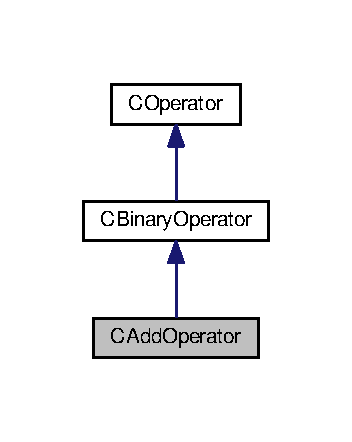
\includegraphics[width=169pt]{classCAddOperator__inherit__graph}
\end{center}
\end{figure}


Collaboration diagram for C\+Add\+Operator\+:\nopagebreak
\begin{figure}[H]
\begin{center}
\leavevmode
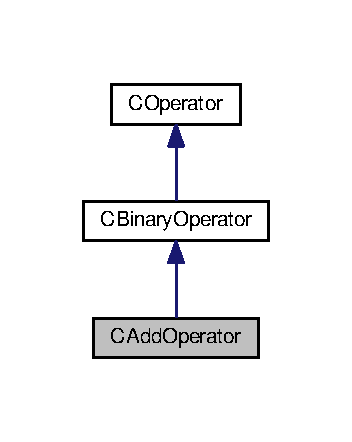
\includegraphics[width=169pt]{classCAddOperator__coll__graph}
\end{center}
\end{figure}
\subsection*{Public Member Functions}
\begin{DoxyCompactItemize}
\item 
\hyperlink{classCAddOperator_aa8b0f16536813f81d9b957a66d540e81}{C\+Add\+Operator} (shared\+\_\+ptr$<$ \hyperlink{classCMatrix}{C\+Matrix} $>$ \&left, shared\+\_\+ptr$<$ \hyperlink{classCMatrix}{C\+Matrix} $>$ \&right)
\item 
\hyperlink{classCMatrix}{C\+Matrix} $\ast$ \hyperlink{classCAddOperator_a7fb8e83b7c5831e3f2e6e8544af49523}{Evaluate} (\hyperlink{classCMemory}{C\+Memory} \&memory) override
\end{DoxyCompactItemize}
\subsection*{Additional Inherited Members}


\subsection{Constructor \& Destructor Documentation}
\index{C\+Add\+Operator@{C\+Add\+Operator}!C\+Add\+Operator@{C\+Add\+Operator}}
\index{C\+Add\+Operator@{C\+Add\+Operator}!C\+Add\+Operator@{C\+Add\+Operator}}
\subsubsection[{\texorpdfstring{C\+Add\+Operator(shared\+\_\+ptr$<$ C\+Matrix $>$ \&left, shared\+\_\+ptr$<$ C\+Matrix $>$ \&right)}{CAddOperator(shared_ptr< CMatrix > &left, shared_ptr< CMatrix > &right)}}]{\setlength{\rightskip}{0pt plus 5cm}C\+Add\+Operator\+::\+C\+Add\+Operator (
\begin{DoxyParamCaption}
\item[{shared\+\_\+ptr$<$ {\bf C\+Matrix} $>$ \&}]{left, }
\item[{shared\+\_\+ptr$<$ {\bf C\+Matrix} $>$ \&}]{right}
\end{DoxyParamCaption}
)\hspace{0.3cm}{\ttfamily [inline]}}\hypertarget{classCAddOperator_aa8b0f16536813f81d9b957a66d540e81}{}\label{classCAddOperator_aa8b0f16536813f81d9b957a66d540e81}


\subsection{Member Function Documentation}
\index{C\+Add\+Operator@{C\+Add\+Operator}!Evaluate@{Evaluate}}
\index{Evaluate@{Evaluate}!C\+Add\+Operator@{C\+Add\+Operator}}
\subsubsection[{\texorpdfstring{Evaluate(\+C\+Memory \&memory) override}{Evaluate(CMemory &memory) override}}]{\setlength{\rightskip}{0pt plus 5cm}{\bf C\+Matrix}$\ast$ C\+Add\+Operator\+::\+Evaluate (
\begin{DoxyParamCaption}
\item[{{\bf C\+Memory} \&}]{memory}
\end{DoxyParamCaption}
)\hspace{0.3cm}{\ttfamily [inline]}, {\ttfamily [override]}, {\ttfamily [virtual]}}\hypertarget{classCAddOperator_a7fb8e83b7c5831e3f2e6e8544af49523}{}\label{classCAddOperator_a7fb8e83b7c5831e3f2e6e8544af49523}


Implements \hyperlink{classCBinaryOperator_aea1eef33f83a4e395091daa0637f4c77}{C\+Binary\+Operator}.



The documentation for this class was generated from the following file\+:\begin{DoxyCompactItemize}
\item 
src/\hyperlink{CAddOperator_8h}{C\+Add\+Operator.\+h}\end{DoxyCompactItemize}

\hypertarget{classCApplication}{}\section{C\+Application Class Reference}
\label{classCApplication}\index{C\+Application@{C\+Application}}


{\ttfamily \#include $<$C\+Application.\+h$>$}



Inheritance diagram for C\+Application\+:\nopagebreak
\begin{figure}[H]
\begin{center}
\leavevmode
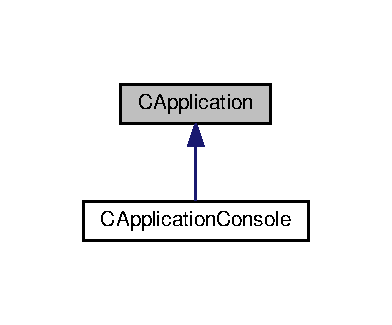
\includegraphics[width=188pt]{classCApplication__inherit__graph}
\end{center}
\end{figure}


Collaboration diagram for C\+Application\+:\nopagebreak
\begin{figure}[H]
\begin{center}
\leavevmode
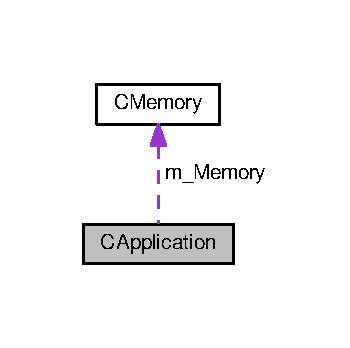
\includegraphics[width=168pt]{classCApplication__coll__graph}
\end{center}
\end{figure}
\subsection*{Public Member Functions}
\begin{DoxyCompactItemize}
\item 
\hyperlink{classCApplication_a186bb7420ce66fadac70d2c30311b6ee}{C\+Application} ()=default
\item 
virtual \hyperlink{classCApplication_ab4448f8a90f380d4ac2afcc9ee59780d}{$\sim$\+C\+Application} ()=default
\item 
bool \hyperlink{classCApplication_a89642c9a6de3ced8f1f77e4fed479e7c}{Evaluate} (string input, string \&result, unique\+\_\+ptr$<$ \hyperlink{classCCommand}{C\+Command} $>$ \&next\+Command)
\item 
void \hyperlink{classCApplication_aa069063a23e53ea9858995f3ca34d6fb}{Run} ()
\item 
virtual void \hyperlink{classCApplication_a5994ba2f7b8a5d88290040616765baaa}{Show\+Var\+Name} (string name) const =0
\item 
virtual void \hyperlink{classCApplication_a8d6b41c059da7fbd01a4857bcb1c06e0}{Show\+Matrix} (unique\+\_\+ptr$<$ \hyperlink{classCMatrix}{C\+Matrix} $>$ \&matrix) const =0
\item 
virtual void \hyperlink{classCApplication_ab88b3a17d0d6e5c14eba88fb263c9857}{Show\+Msg} (string msg) const =0
\end{DoxyCompactItemize}
\subsection*{Protected Member Functions}
\begin{DoxyCompactItemize}
\item 
virtual void \hyperlink{classCApplication_a308f31081c5a2b880c1bc96dbac3260d}{Print\+Instructions} () const =0
\item 
virtual string \hyperlink{classCApplication_a69a1706c3cf78d8dad7e16734e92b3f6}{Get\+Input} () const =0
\item 
virtual bool \hyperlink{classCApplication_ae2fe7afcd1a15cdbf5eb97a69b7731e6}{Parse\+Command} (string \&input, unique\+\_\+ptr$<$ \hyperlink{classCCommand}{C\+Command} $>$ \&next\+Command)=0
\item 
virtual void \hyperlink{classCApplication_a13cc1aa745b5b4c4d7e02a77a1bbdac8}{Show\+Result} (string result)=0
\end{DoxyCompactItemize}
\subsection*{Protected Attributes}
\begin{DoxyCompactItemize}
\item 
\hyperlink{classCMemory}{C\+Memory} \hyperlink{classCApplication_a338eac28666e5f1577716eb7097ffadb}{m\+\_\+\+Memory}
\end{DoxyCompactItemize}


\subsection{Constructor \& Destructor Documentation}
\index{C\+Application@{C\+Application}!C\+Application@{C\+Application}}
\index{C\+Application@{C\+Application}!C\+Application@{C\+Application}}
\subsubsection[{\texorpdfstring{C\+Application()=default}{CApplication()=default}}]{\setlength{\rightskip}{0pt plus 5cm}C\+Application\+::\+C\+Application (
\begin{DoxyParamCaption}
{}
\end{DoxyParamCaption}
)\hspace{0.3cm}{\ttfamily [default]}}\hypertarget{classCApplication_a186bb7420ce66fadac70d2c30311b6ee}{}\label{classCApplication_a186bb7420ce66fadac70d2c30311b6ee}
\index{C\+Application@{C\+Application}!````~C\+Application@{$\sim$\+C\+Application}}
\index{````~C\+Application@{$\sim$\+C\+Application}!C\+Application@{C\+Application}}
\subsubsection[{\texorpdfstring{$\sim$\+C\+Application()=default}{~CApplication()=default}}]{\setlength{\rightskip}{0pt plus 5cm}virtual C\+Application\+::$\sim$\+C\+Application (
\begin{DoxyParamCaption}
{}
\end{DoxyParamCaption}
)\hspace{0.3cm}{\ttfamily [virtual]}, {\ttfamily [default]}}\hypertarget{classCApplication_ab4448f8a90f380d4ac2afcc9ee59780d}{}\label{classCApplication_ab4448f8a90f380d4ac2afcc9ee59780d}


\subsection{Member Function Documentation}
\index{C\+Application@{C\+Application}!Evaluate@{Evaluate}}
\index{Evaluate@{Evaluate}!C\+Application@{C\+Application}}
\subsubsection[{\texorpdfstring{Evaluate(string input, string \&result, unique\+\_\+ptr$<$ C\+Command $>$ \&next\+Command)}{Evaluate(string input, string &result, unique_ptr< CCommand > &nextCommand)}}]{\setlength{\rightskip}{0pt plus 5cm}bool C\+Application\+::\+Evaluate (
\begin{DoxyParamCaption}
\item[{string}]{input, }
\item[{string \&}]{result, }
\item[{unique\+\_\+ptr$<$ {\bf C\+Command} $>$ \&}]{next\+Command}
\end{DoxyParamCaption}
)\hspace{0.3cm}{\ttfamily [inline]}}\hypertarget{classCApplication_a89642c9a6de3ced8f1f77e4fed479e7c}{}\label{classCApplication_a89642c9a6de3ced8f1f77e4fed479e7c}
\index{C\+Application@{C\+Application}!Get\+Input@{Get\+Input}}
\index{Get\+Input@{Get\+Input}!C\+Application@{C\+Application}}
\subsubsection[{\texorpdfstring{Get\+Input() const =0}{GetInput() const =0}}]{\setlength{\rightskip}{0pt plus 5cm}virtual string C\+Application\+::\+Get\+Input (
\begin{DoxyParamCaption}
{}
\end{DoxyParamCaption}
) const\hspace{0.3cm}{\ttfamily [protected]}, {\ttfamily [pure virtual]}}\hypertarget{classCApplication_a69a1706c3cf78d8dad7e16734e92b3f6}{}\label{classCApplication_a69a1706c3cf78d8dad7e16734e92b3f6}


Implemented in \hyperlink{classCApplicationConsole_a0af959fae7259bf81f7855985e16adff}{C\+Application\+Console}.

\index{C\+Application@{C\+Application}!Parse\+Command@{Parse\+Command}}
\index{Parse\+Command@{Parse\+Command}!C\+Application@{C\+Application}}
\subsubsection[{\texorpdfstring{Parse\+Command(string \&input, unique\+\_\+ptr$<$ C\+Command $>$ \&next\+Command)=0}{ParseCommand(string &input, unique_ptr< CCommand > &nextCommand)=0}}]{\setlength{\rightskip}{0pt plus 5cm}virtual bool C\+Application\+::\+Parse\+Command (
\begin{DoxyParamCaption}
\item[{string \&}]{input, }
\item[{unique\+\_\+ptr$<$ {\bf C\+Command} $>$ \&}]{next\+Command}
\end{DoxyParamCaption}
)\hspace{0.3cm}{\ttfamily [protected]}, {\ttfamily [pure virtual]}}\hypertarget{classCApplication_ae2fe7afcd1a15cdbf5eb97a69b7731e6}{}\label{classCApplication_ae2fe7afcd1a15cdbf5eb97a69b7731e6}


Implemented in \hyperlink{classCApplicationConsole_ae2ee7085fd41f96607d37673ed705e76}{C\+Application\+Console}.

\index{C\+Application@{C\+Application}!Print\+Instructions@{Print\+Instructions}}
\index{Print\+Instructions@{Print\+Instructions}!C\+Application@{C\+Application}}
\subsubsection[{\texorpdfstring{Print\+Instructions() const =0}{PrintInstructions() const =0}}]{\setlength{\rightskip}{0pt plus 5cm}virtual void C\+Application\+::\+Print\+Instructions (
\begin{DoxyParamCaption}
{}
\end{DoxyParamCaption}
) const\hspace{0.3cm}{\ttfamily [protected]}, {\ttfamily [pure virtual]}}\hypertarget{classCApplication_a308f31081c5a2b880c1bc96dbac3260d}{}\label{classCApplication_a308f31081c5a2b880c1bc96dbac3260d}


Implemented in \hyperlink{classCApplicationConsole_a77c169050d8faff5ff4019d3204e6ff8}{C\+Application\+Console}.

\index{C\+Application@{C\+Application}!Run@{Run}}
\index{Run@{Run}!C\+Application@{C\+Application}}
\subsubsection[{\texorpdfstring{Run()}{Run()}}]{\setlength{\rightskip}{0pt plus 5cm}void C\+Application\+::\+Run (
\begin{DoxyParamCaption}
{}
\end{DoxyParamCaption}
)\hspace{0.3cm}{\ttfamily [inline]}}\hypertarget{classCApplication_aa069063a23e53ea9858995f3ca34d6fb}{}\label{classCApplication_aa069063a23e53ea9858995f3ca34d6fb}
\index{C\+Application@{C\+Application}!Show\+Matrix@{Show\+Matrix}}
\index{Show\+Matrix@{Show\+Matrix}!C\+Application@{C\+Application}}
\subsubsection[{\texorpdfstring{Show\+Matrix(unique\+\_\+ptr$<$ C\+Matrix $>$ \&matrix) const =0}{ShowMatrix(unique_ptr< CMatrix > &matrix) const =0}}]{\setlength{\rightskip}{0pt plus 5cm}virtual void C\+Application\+::\+Show\+Matrix (
\begin{DoxyParamCaption}
\item[{unique\+\_\+ptr$<$ {\bf C\+Matrix} $>$ \&}]{matrix}
\end{DoxyParamCaption}
) const\hspace{0.3cm}{\ttfamily [pure virtual]}}\hypertarget{classCApplication_a8d6b41c059da7fbd01a4857bcb1c06e0}{}\label{classCApplication_a8d6b41c059da7fbd01a4857bcb1c06e0}


Implemented in \hyperlink{classCApplicationConsole_a7c024277c01acd4cc575ad64ffd07a22}{C\+Application\+Console}.

\index{C\+Application@{C\+Application}!Show\+Msg@{Show\+Msg}}
\index{Show\+Msg@{Show\+Msg}!C\+Application@{C\+Application}}
\subsubsection[{\texorpdfstring{Show\+Msg(string msg) const =0}{ShowMsg(string msg) const =0}}]{\setlength{\rightskip}{0pt plus 5cm}virtual void C\+Application\+::\+Show\+Msg (
\begin{DoxyParamCaption}
\item[{string}]{msg}
\end{DoxyParamCaption}
) const\hspace{0.3cm}{\ttfamily [pure virtual]}}\hypertarget{classCApplication_ab88b3a17d0d6e5c14eba88fb263c9857}{}\label{classCApplication_ab88b3a17d0d6e5c14eba88fb263c9857}


Implemented in \hyperlink{classCApplicationConsole_a32152dd2a1793b20fd03ba3179d8e22e}{C\+Application\+Console}.

\index{C\+Application@{C\+Application}!Show\+Result@{Show\+Result}}
\index{Show\+Result@{Show\+Result}!C\+Application@{C\+Application}}
\subsubsection[{\texorpdfstring{Show\+Result(string result)=0}{ShowResult(string result)=0}}]{\setlength{\rightskip}{0pt plus 5cm}virtual void C\+Application\+::\+Show\+Result (
\begin{DoxyParamCaption}
\item[{string}]{result}
\end{DoxyParamCaption}
)\hspace{0.3cm}{\ttfamily [protected]}, {\ttfamily [pure virtual]}}\hypertarget{classCApplication_a13cc1aa745b5b4c4d7e02a77a1bbdac8}{}\label{classCApplication_a13cc1aa745b5b4c4d7e02a77a1bbdac8}


Implemented in \hyperlink{classCApplicationConsole_a311cfc33ddf26daa5f6a759a335ea007}{C\+Application\+Console}.

\index{C\+Application@{C\+Application}!Show\+Var\+Name@{Show\+Var\+Name}}
\index{Show\+Var\+Name@{Show\+Var\+Name}!C\+Application@{C\+Application}}
\subsubsection[{\texorpdfstring{Show\+Var\+Name(string name) const =0}{ShowVarName(string name) const =0}}]{\setlength{\rightskip}{0pt plus 5cm}virtual void C\+Application\+::\+Show\+Var\+Name (
\begin{DoxyParamCaption}
\item[{string}]{name}
\end{DoxyParamCaption}
) const\hspace{0.3cm}{\ttfamily [pure virtual]}}\hypertarget{classCApplication_a5994ba2f7b8a5d88290040616765baaa}{}\label{classCApplication_a5994ba2f7b8a5d88290040616765baaa}


Implemented in \hyperlink{classCApplicationConsole_a20c9dbcb6b56834b28ff9909f446848f}{C\+Application\+Console}.



\subsection{Member Data Documentation}
\index{C\+Application@{C\+Application}!m\+\_\+\+Memory@{m\+\_\+\+Memory}}
\index{m\+\_\+\+Memory@{m\+\_\+\+Memory}!C\+Application@{C\+Application}}
\subsubsection[{\texorpdfstring{m\+\_\+\+Memory}{m_Memory}}]{\setlength{\rightskip}{0pt plus 5cm}{\bf C\+Memory} C\+Application\+::m\+\_\+\+Memory\hspace{0.3cm}{\ttfamily [protected]}}\hypertarget{classCApplication_a338eac28666e5f1577716eb7097ffadb}{}\label{classCApplication_a338eac28666e5f1577716eb7097ffadb}


The documentation for this class was generated from the following file\+:\begin{DoxyCompactItemize}
\item 
src/\hyperlink{CApplication_8h}{C\+Application.\+h}\end{DoxyCompactItemize}

\hypertarget{classCApplicationConsole}{}\section{C\+Application\+Console Class Reference}
\label{classCApplicationConsole}\index{C\+Application\+Console@{C\+Application\+Console}}


{\ttfamily \#include $<$C\+Application\+Console.\+h$>$}



Inheritance diagram for C\+Application\+Console\+:\nopagebreak
\begin{figure}[H]
\begin{center}
\leavevmode
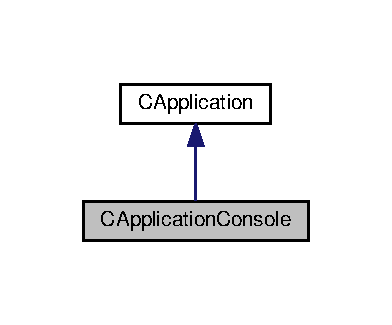
\includegraphics[width=188pt]{classCApplicationConsole__inherit__graph}
\end{center}
\end{figure}


Collaboration diagram for C\+Application\+Console\+:\nopagebreak
\begin{figure}[H]
\begin{center}
\leavevmode
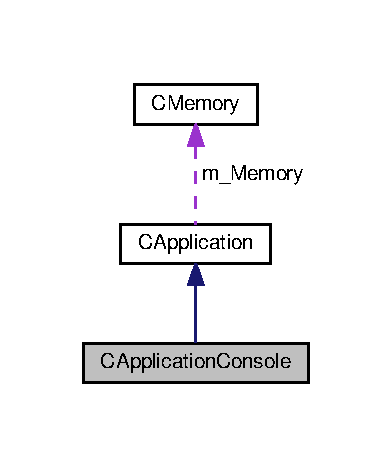
\includegraphics[width=188pt]{classCApplicationConsole__coll__graph}
\end{center}
\end{figure}
\subsection*{Public Member Functions}
\begin{DoxyCompactItemize}
\item 
\hyperlink{classCApplicationConsole_a5d2e88210a41c621fbfb933eedb181b1}{C\+Application\+Console} ()
\item 
\hyperlink{classCApplicationConsole_ab06aed70666ce71431eb314dfcadb35e}{$\sim$\+C\+Application\+Console} () override=default
\item 
void \hyperlink{classCApplicationConsole_a77c169050d8faff5ff4019d3204e6ff8}{Print\+Instructions} () const override
\end{DoxyCompactItemize}
\subsection*{Private Member Functions}
\begin{DoxyCompactItemize}
\item 
string \hyperlink{classCApplicationConsole_a0af959fae7259bf81f7855985e16adff}{Get\+Input} () const override
\item 
void \hyperlink{classCApplicationConsole_a32152dd2a1793b20fd03ba3179d8e22e}{Show\+Msg} (string msg) const override
\item 
void \hyperlink{classCApplicationConsole_ad9d3e1cdadd2cc2e89dfa3591942f5f3}{Show\+Help} () const override
\item 
bool \hyperlink{classCApplicationConsole_a95f0c288b2224cc1273cf20472cbc34f}{get\+Variable\+Name} (string \&input, string \&var\+Name) const 
\item 
bool \hyperlink{classCApplicationConsole_a1444353413fae5d03ba68a803f724379}{Read\+Size} (std\+::size\+\_\+t \&num\+Rows, std\+::size\+\_\+t \&num\+Cols, istream \&in\+Stream) const 
\item 
bool \hyperlink{classCApplicationConsole_a2323e596b3a019fe843f88955218baba}{Read\+Matrix} (istream \&in\+Stream, vector$<$ vector$<$ double $>$$>$ \&matrix, size\+\_\+t num\+Rows, size\+\_\+t num\+Cols) const 
\item 
bool \hyperlink{classCApplicationConsole_a6ca78c0250dfbdf71a995277c0485e5a}{Is\+Syntax\+Correct} (istream \&in\+Stream) const 
\item 
void \hyperlink{classCApplicationConsole_a4bca66a2f575557ca929d2fa8c8f9028}{Show\+Result} (string result) const override
\item 
bool \hyperlink{classCApplicationConsole_a4ae836d72b1ecdc4b3c3e15ff5f171b6}{Parse\+Command\+Word} (string \&input, string \&in\+\_\+command)
\item 
bool \hyperlink{classCApplicationConsole_ab17d9e0bf16052fff75f721f9aaaafc8}{Parse\+Command} (string \&input, unique\+\_\+ptr$<$ \hyperlink{classCCommand}{C\+Command} $>$ \&command) override
\item 
bool \hyperlink{classCApplicationConsole_a12531e44827274807a3a0787e66345fe}{Load\+Operand\+Name} (string \&input, string \&name)
\item 
bool \hyperlink{classCApplicationConsole_a092af2533775a460a05e7c5198d991fa}{Parse\+Loading} (string \&input, string \&var\+Name, vector$<$ vector$<$ double $>$$>$ \&matrix\+Nums)
\item 
bool \hyperlink{classCApplicationConsole_a00a40d89b87f545373a7ce3d22a7c996}{Parse\+Operands} (string \&input, vector$<$ string $>$ \&operands, std\+::size\+\_\+t num\+Of\+Operands=1)
\item 
bool \hyperlink{classCApplicationConsole_ae3c29fe61ba160f51ead41382df8c494}{Parse\+Cutting} (string \&input, string \&var\+Name, std\+::size\+\_\+t \&num\+Rows, size\+\_\+t \&num\+Cols, pair$<$ size\+\_\+t, size\+\_\+t $>$ \&start\+Point)
\end{DoxyCompactItemize}
\subsection*{Additional Inherited Members}


\subsection{Constructor \& Destructor Documentation}
\index{C\+Application\+Console@{C\+Application\+Console}!C\+Application\+Console@{C\+Application\+Console}}
\index{C\+Application\+Console@{C\+Application\+Console}!C\+Application\+Console@{C\+Application\+Console}}
\subsubsection[{\texorpdfstring{C\+Application\+Console()}{CApplicationConsole()}}]{\setlength{\rightskip}{0pt plus 5cm}C\+Application\+Console\+::\+C\+Application\+Console (
\begin{DoxyParamCaption}
{}
\end{DoxyParamCaption}
)\hspace{0.3cm}{\ttfamily [inline]}}\hypertarget{classCApplicationConsole_a5d2e88210a41c621fbfb933eedb181b1}{}\label{classCApplicationConsole_a5d2e88210a41c621fbfb933eedb181b1}
\index{C\+Application\+Console@{C\+Application\+Console}!````~C\+Application\+Console@{$\sim$\+C\+Application\+Console}}
\index{````~C\+Application\+Console@{$\sim$\+C\+Application\+Console}!C\+Application\+Console@{C\+Application\+Console}}
\subsubsection[{\texorpdfstring{$\sim$\+C\+Application\+Console() override=default}{~CApplicationConsole() override=default}}]{\setlength{\rightskip}{0pt plus 5cm}C\+Application\+Console\+::$\sim$\+C\+Application\+Console (
\begin{DoxyParamCaption}
{}
\end{DoxyParamCaption}
)\hspace{0.3cm}{\ttfamily [override]}, {\ttfamily [default]}}\hypertarget{classCApplicationConsole_ab06aed70666ce71431eb314dfcadb35e}{}\label{classCApplicationConsole_ab06aed70666ce71431eb314dfcadb35e}


\subsection{Member Function Documentation}
\index{C\+Application\+Console@{C\+Application\+Console}!Get\+Input@{Get\+Input}}
\index{Get\+Input@{Get\+Input}!C\+Application\+Console@{C\+Application\+Console}}
\subsubsection[{\texorpdfstring{Get\+Input() const override}{GetInput() const override}}]{\setlength{\rightskip}{0pt plus 5cm}string C\+Application\+Console\+::\+Get\+Input (
\begin{DoxyParamCaption}
{}
\end{DoxyParamCaption}
) const\hspace{0.3cm}{\ttfamily [override]}, {\ttfamily [private]}, {\ttfamily [virtual]}}\hypertarget{classCApplicationConsole_a0af959fae7259bf81f7855985e16adff}{}\label{classCApplicationConsole_a0af959fae7259bf81f7855985e16adff}
Get input from user. \begin{DoxyReturn}{Returns}
input data in string 
\end{DoxyReturn}


Implements \hyperlink{classCApplication_a69a1706c3cf78d8dad7e16734e92b3f6}{C\+Application}.

\index{C\+Application\+Console@{C\+Application\+Console}!get\+Variable\+Name@{get\+Variable\+Name}}
\index{get\+Variable\+Name@{get\+Variable\+Name}!C\+Application\+Console@{C\+Application\+Console}}
\subsubsection[{\texorpdfstring{get\+Variable\+Name(string \&input, string \&var\+Name) const }{getVariableName(string &input, string &varName) const }}]{\setlength{\rightskip}{0pt plus 5cm}bool C\+Application\+Console\+::get\+Variable\+Name (
\begin{DoxyParamCaption}
\item[{string \&}]{input, }
\item[{string \&}]{var\+Name}
\end{DoxyParamCaption}
) const\hspace{0.3cm}{\ttfamily [private]}}\hypertarget{classCApplicationConsole_a95f0c288b2224cc1273cf20472cbc34f}{}\label{classCApplicationConsole_a95f0c288b2224cc1273cf20472cbc34f}
Read name of a variable from input. 
\begin{DoxyParams}{Parameters}
{\em input} & input data \\
\hline
{\em var\+Name} & name of variable \\
\hline
\end{DoxyParams}
\begin{DoxyReturn}{Returns}
true if variable name read successfully, false otherwise (incorrect syntax) 
\end{DoxyReturn}
\index{C\+Application\+Console@{C\+Application\+Console}!Is\+Syntax\+Correct@{Is\+Syntax\+Correct}}
\index{Is\+Syntax\+Correct@{Is\+Syntax\+Correct}!C\+Application\+Console@{C\+Application\+Console}}
\subsubsection[{\texorpdfstring{Is\+Syntax\+Correct(istream \&in\+Stream) const }{IsSyntaxCorrect(istream &inStream) const }}]{\setlength{\rightskip}{0pt plus 5cm}bool C\+Application\+Console\+::\+Is\+Syntax\+Correct (
\begin{DoxyParamCaption}
\item[{istream \&}]{in\+Stream}
\end{DoxyParamCaption}
) const\hspace{0.3cm}{\ttfamily [inline]}, {\ttfamily [private]}}\hypertarget{classCApplicationConsole_a6ca78c0250dfbdf71a995277c0485e5a}{}\label{classCApplicationConsole_a6ca78c0250dfbdf71a995277c0485e5a}
Check if command is properly ended. 
\begin{DoxyParams}{Parameters}
{\em in\+Stream} & input stream \\
\hline
\end{DoxyParams}
\begin{DoxyReturn}{Returns}
true if properly ended 
\end{DoxyReturn}
\index{C\+Application\+Console@{C\+Application\+Console}!Load\+Operand\+Name@{Load\+Operand\+Name}}
\index{Load\+Operand\+Name@{Load\+Operand\+Name}!C\+Application\+Console@{C\+Application\+Console}}
\subsubsection[{\texorpdfstring{Load\+Operand\+Name(string \&input, string \&name)}{LoadOperandName(string &input, string &name)}}]{\setlength{\rightskip}{0pt plus 5cm}bool C\+Application\+Console\+::\+Load\+Operand\+Name (
\begin{DoxyParamCaption}
\item[{string \&}]{input, }
\item[{string \&}]{name}
\end{DoxyParamCaption}
)\hspace{0.3cm}{\ttfamily [inline]}, {\ttfamily [private]}}\hypertarget{classCApplicationConsole_a12531e44827274807a3a0787e66345fe}{}\label{classCApplicationConsole_a12531e44827274807a3a0787e66345fe}
Load name of operand variable. 
\begin{DoxyParams}{Parameters}
{\em input} & input data \\
\hline
{\em name} & variable name \\
\hline
\end{DoxyParams}
\begin{DoxyReturn}{Returns}
true if loaded successfully, false otherwise (incorrect syntax) 
\end{DoxyReturn}
\index{C\+Application\+Console@{C\+Application\+Console}!Parse\+Command@{Parse\+Command}}
\index{Parse\+Command@{Parse\+Command}!C\+Application\+Console@{C\+Application\+Console}}
\subsubsection[{\texorpdfstring{Parse\+Command(string \&input, unique\+\_\+ptr$<$ C\+Command $>$ \&command) override}{ParseCommand(string &input, unique_ptr< CCommand > &command) override}}]{\setlength{\rightskip}{0pt plus 5cm}bool C\+Application\+Console\+::\+Parse\+Command (
\begin{DoxyParamCaption}
\item[{string \&}]{input, }
\item[{unique\+\_\+ptr$<$ {\bf C\+Command} $>$ \&}]{command}
\end{DoxyParamCaption}
)\hspace{0.3cm}{\ttfamily [inline]}, {\ttfamily [override]}, {\ttfamily [private]}, {\ttfamily [virtual]}}\hypertarget{classCApplicationConsole_ab17d9e0bf16052fff75f721f9aaaafc8}{}\label{classCApplicationConsole_ab17d9e0bf16052fff75f721f9aaaafc8}
Parse input data into commands. 
\begin{DoxyParams}{Parameters}
{\em input} & input data \\
\hline
{\em command} & parsed command \\
\hline
\end{DoxyParams}
\begin{DoxyReturn}{Returns}
true if command successfully parsed, false otherwise 
\end{DoxyReturn}


Implements \hyperlink{classCApplication_abfa3357f4517c85261fac0bc307e1ab7}{C\+Application}.

\index{C\+Application\+Console@{C\+Application\+Console}!Parse\+Command\+Word@{Parse\+Command\+Word}}
\index{Parse\+Command\+Word@{Parse\+Command\+Word}!C\+Application\+Console@{C\+Application\+Console}}
\subsubsection[{\texorpdfstring{Parse\+Command\+Word(string \&input, string \&in\+\_\+command)}{ParseCommandWord(string &input, string &in_command)}}]{\setlength{\rightskip}{0pt plus 5cm}bool C\+Application\+Console\+::\+Parse\+Command\+Word (
\begin{DoxyParamCaption}
\item[{string \&}]{input, }
\item[{string \&}]{in\+\_\+command}
\end{DoxyParamCaption}
)\hspace{0.3cm}{\ttfamily [inline]}, {\ttfamily [private]}}\hypertarget{classCApplicationConsole_a4ae836d72b1ecdc4b3c3e15ff5f171b6}{}\label{classCApplicationConsole_a4ae836d72b1ecdc4b3c3e15ff5f171b6}
Parse name of the command from input. 
\begin{DoxyParams}{Parameters}
{\em input} & input data \\
\hline
{\em in\+\_\+command} & name of the command \\
\hline
\end{DoxyParams}
\begin{DoxyReturn}{Returns}
true if parsed successfully, false otherwise (incorrect syntax) 
\end{DoxyReturn}
\index{C\+Application\+Console@{C\+Application\+Console}!Parse\+Cutting@{Parse\+Cutting}}
\index{Parse\+Cutting@{Parse\+Cutting}!C\+Application\+Console@{C\+Application\+Console}}
\subsubsection[{\texorpdfstring{Parse\+Cutting(string \&input, string \&var\+Name, std\+::size\+\_\+t \&num\+Rows, size\+\_\+t \&num\+Cols, pair$<$ size\+\_\+t, size\+\_\+t $>$ \&start\+Point)}{ParseCutting(string &input, string &varName, std::size_t &numRows, size_t &numCols, pair< size_t, size_t > &startPoint)}}]{\setlength{\rightskip}{0pt plus 5cm}bool C\+Application\+Console\+::\+Parse\+Cutting (
\begin{DoxyParamCaption}
\item[{string \&}]{input, }
\item[{string \&}]{var\+Name, }
\item[{std\+::size\+\_\+t \&}]{num\+Rows, }
\item[{size\+\_\+t \&}]{num\+Cols, }
\item[{pair$<$ size\+\_\+t, size\+\_\+t $>$ \&}]{start\+Point}
\end{DoxyParamCaption}
)\hspace{0.3cm}{\ttfamily [inline]}, {\ttfamily [private]}}\hypertarget{classCApplicationConsole_ae3c29fe61ba160f51ead41382df8c494}{}\label{classCApplicationConsole_ae3c29fe61ba160f51ead41382df8c494}
Parse parameters for cutting of a matrix. 
\begin{DoxyParams}{Parameters}
{\em input} & input data \\
\hline
{\em var\+Name} & input variable name \\
\hline
{\em num\+Rows} & number of rows of the cut matrix \\
\hline
{\em num\+Cols} & number of columns of the cut matrix \\
\hline
{\em start\+Point} & row and column index where to start cutting \\
\hline
\end{DoxyParams}
\begin{DoxyReturn}{Returns}
true if successful, false otherwise (incorrect syntax) 
\end{DoxyReturn}
\index{C\+Application\+Console@{C\+Application\+Console}!Parse\+Loading@{Parse\+Loading}}
\index{Parse\+Loading@{Parse\+Loading}!C\+Application\+Console@{C\+Application\+Console}}
\subsubsection[{\texorpdfstring{Parse\+Loading(string \&input, string \&var\+Name, vector$<$ vector$<$ double $>$$>$ \&matrix\+Nums)}{ParseLoading(string &input, string &varName, vector< vector< double >> &matrixNums)}}]{\setlength{\rightskip}{0pt plus 5cm}bool C\+Application\+Console\+::\+Parse\+Loading (
\begin{DoxyParamCaption}
\item[{string \&}]{input, }
\item[{string \&}]{var\+Name, }
\item[{vector$<$ vector$<$ double $>$$>$ \&}]{matrix\+Nums}
\end{DoxyParamCaption}
)\hspace{0.3cm}{\ttfamily [inline]}, {\ttfamily [private]}}\hypertarget{classCApplicationConsole_a092af2533775a460a05e7c5198d991fa}{}\label{classCApplicationConsole_a092af2533775a460a05e7c5198d991fa}
Parse parameters for loading of a matrix. 
\begin{DoxyParams}{Parameters}
{\em input} & input data \\
\hline
{\em var\+Name} & name of variable to be loaded \\
\hline
{\em matrix\+Nums} & values of a loaded matrix \\
\hline
\end{DoxyParams}
\begin{DoxyReturn}{Returns}
true if successful, false otherwise (incorrect syntax) 
\end{DoxyReturn}
\index{C\+Application\+Console@{C\+Application\+Console}!Parse\+Operands@{Parse\+Operands}}
\index{Parse\+Operands@{Parse\+Operands}!C\+Application\+Console@{C\+Application\+Console}}
\subsubsection[{\texorpdfstring{Parse\+Operands(string \&input, vector$<$ string $>$ \&operands, std\+::size\+\_\+t num\+Of\+Operands=1)}{ParseOperands(string &input, vector< string > &operands, std::size_t numOfOperands=1)}}]{\setlength{\rightskip}{0pt plus 5cm}bool C\+Application\+Console\+::\+Parse\+Operands (
\begin{DoxyParamCaption}
\item[{string \&}]{input, }
\item[{vector$<$ string $>$ \&}]{operands, }
\item[{std\+::size\+\_\+t}]{num\+Of\+Operands = {\ttfamily 1}}
\end{DoxyParamCaption}
)\hspace{0.3cm}{\ttfamily [inline]}, {\ttfamily [private]}}\hypertarget{classCApplicationConsole_a00a40d89b87f545373a7ce3d22a7c996}{}\label{classCApplicationConsole_a00a40d89b87f545373a7ce3d22a7c996}
Parse operand variable names. 
\begin{DoxyParams}{Parameters}
{\em input} & input data \\
\hline
{\em operands} & vector to store operands \\
\hline
{\em num\+Of\+Operands} & number of operands to parse \\
\hline
\end{DoxyParams}
\begin{DoxyReturn}{Returns}
true if successfull, false otherwise (incorrect syntax) 
\end{DoxyReturn}
\index{C\+Application\+Console@{C\+Application\+Console}!Print\+Instructions@{Print\+Instructions}}
\index{Print\+Instructions@{Print\+Instructions}!C\+Application\+Console@{C\+Application\+Console}}
\subsubsection[{\texorpdfstring{Print\+Instructions() const override}{PrintInstructions() const override}}]{\setlength{\rightskip}{0pt plus 5cm}void C\+Application\+Console\+::\+Print\+Instructions (
\begin{DoxyParamCaption}
{}
\end{DoxyParamCaption}
) const\hspace{0.3cm}{\ttfamily [inline]}, {\ttfamily [override]}, {\ttfamily [virtual]}}\hypertarget{classCApplicationConsole_a77c169050d8faff5ff4019d3204e6ff8}{}\label{classCApplicationConsole_a77c169050d8faff5ff4019d3204e6ff8}
Shoq basic usage instructions on the screen. 

Implements \hyperlink{classCApplication_a308f31081c5a2b880c1bc96dbac3260d}{C\+Application}.

\index{C\+Application\+Console@{C\+Application\+Console}!Read\+Matrix@{Read\+Matrix}}
\index{Read\+Matrix@{Read\+Matrix}!C\+Application\+Console@{C\+Application\+Console}}
\subsubsection[{\texorpdfstring{Read\+Matrix(istream \&in\+Stream, vector$<$ vector$<$ double $>$$>$ \&matrix, size\+\_\+t num\+Rows, size\+\_\+t num\+Cols) const }{ReadMatrix(istream &inStream, vector< vector< double >> &matrix, size_t numRows, size_t numCols) const }}]{\setlength{\rightskip}{0pt plus 5cm}bool C\+Application\+Console\+::\+Read\+Matrix (
\begin{DoxyParamCaption}
\item[{istream \&}]{in\+Stream, }
\item[{vector$<$ vector$<$ double $>$$>$ \&}]{matrix, }
\item[{size\+\_\+t}]{num\+Rows, }
\item[{size\+\_\+t}]{num\+Cols}
\end{DoxyParamCaption}
) const\hspace{0.3cm}{\ttfamily [private]}}\hypertarget{classCApplicationConsole_a2323e596b3a019fe843f88955218baba}{}\label{classCApplicationConsole_a2323e596b3a019fe843f88955218baba}
Read and set values of a matrix from a stream. 
\begin{DoxyParams}{Parameters}
{\em in\+Stream} & input stream \\
\hline
{\em matrix} & values of matrix to be set \\
\hline
{\em num\+Rows} & number of rows of the matrix \\
\hline
{\em num\+Cols} & number of columns of the matrix \\
\hline
\end{DoxyParams}
\begin{DoxyReturn}{Returns}
true if read successfully, false otherwise (wrong number of values) 
\end{DoxyReturn}
\index{C\+Application\+Console@{C\+Application\+Console}!Read\+Size@{Read\+Size}}
\index{Read\+Size@{Read\+Size}!C\+Application\+Console@{C\+Application\+Console}}
\subsubsection[{\texorpdfstring{Read\+Size(std\+::size\+\_\+t \&num\+Rows, std\+::size\+\_\+t \&num\+Cols, istream \&in\+Stream) const }{ReadSize(std::size_t &numRows, std::size_t &numCols, istream &inStream) const }}]{\setlength{\rightskip}{0pt plus 5cm}bool C\+Application\+Console\+::\+Read\+Size (
\begin{DoxyParamCaption}
\item[{std\+::size\+\_\+t \&}]{num\+Rows, }
\item[{std\+::size\+\_\+t \&}]{num\+Cols, }
\item[{istream \&}]{in\+Stream}
\end{DoxyParamCaption}
) const\hspace{0.3cm}{\ttfamily [private]}}\hypertarget{classCApplicationConsole_a1444353413fae5d03ba68a803f724379}{}\label{classCApplicationConsole_a1444353413fae5d03ba68a803f724379}
Read size of result matrix from input. 
\begin{DoxyParams}{Parameters}
{\em num\+Rows} & number of rows \\
\hline
{\em num\+Cols} & number of columns \\
\hline
{\em in\+Stream} & input stream \\
\hline
\end{DoxyParams}
\begin{DoxyReturn}{Returns}
true if read successfully, false otherwise (incorrect syntax) 
\end{DoxyReturn}
\index{C\+Application\+Console@{C\+Application\+Console}!Show\+Help@{Show\+Help}}
\index{Show\+Help@{Show\+Help}!C\+Application\+Console@{C\+Application\+Console}}
\subsubsection[{\texorpdfstring{Show\+Help() const override}{ShowHelp() const override}}]{\setlength{\rightskip}{0pt plus 5cm}void C\+Application\+Console\+::\+Show\+Help (
\begin{DoxyParamCaption}
{}
\end{DoxyParamCaption}
) const\hspace{0.3cm}{\ttfamily [inline]}, {\ttfamily [override]}, {\ttfamily [private]}, {\ttfamily [virtual]}}\hypertarget{classCApplicationConsole_ad9d3e1cdadd2cc2e89dfa3591942f5f3}{}\label{classCApplicationConsole_ad9d3e1cdadd2cc2e89dfa3591942f5f3}
Show description of app commands on the screen. 

Implements \hyperlink{classCApplication_a97b87502b1a3c7fdaa7d8ef2e7870eaf}{C\+Application}.

\index{C\+Application\+Console@{C\+Application\+Console}!Show\+Msg@{Show\+Msg}}
\index{Show\+Msg@{Show\+Msg}!C\+Application\+Console@{C\+Application\+Console}}
\subsubsection[{\texorpdfstring{Show\+Msg(string msg) const override}{ShowMsg(string msg) const override}}]{\setlength{\rightskip}{0pt plus 5cm}void C\+Application\+Console\+::\+Show\+Msg (
\begin{DoxyParamCaption}
\item[{string}]{msg}
\end{DoxyParamCaption}
) const\hspace{0.3cm}{\ttfamily [inline]}, {\ttfamily [override]}, {\ttfamily [private]}, {\ttfamily [virtual]}}\hypertarget{classCApplicationConsole_a32152dd2a1793b20fd03ba3179d8e22e}{}\label{classCApplicationConsole_a32152dd2a1793b20fd03ba3179d8e22e}
Show message on the screen. 
\begin{DoxyParams}{Parameters}
{\em msg} & message to be shown \\
\hline
\end{DoxyParams}


Implements \hyperlink{classCApplication_ab88b3a17d0d6e5c14eba88fb263c9857}{C\+Application}.

\index{C\+Application\+Console@{C\+Application\+Console}!Show\+Result@{Show\+Result}}
\index{Show\+Result@{Show\+Result}!C\+Application\+Console@{C\+Application\+Console}}
\subsubsection[{\texorpdfstring{Show\+Result(string result) const override}{ShowResult(string result) const override}}]{\setlength{\rightskip}{0pt plus 5cm}void C\+Application\+Console\+::\+Show\+Result (
\begin{DoxyParamCaption}
\item[{string}]{result}
\end{DoxyParamCaption}
) const\hspace{0.3cm}{\ttfamily [inline]}, {\ttfamily [override]}, {\ttfamily [private]}, {\ttfamily [virtual]}}\hypertarget{classCApplicationConsole_a4bca66a2f575557ca929d2fa8c8f9028}{}\label{classCApplicationConsole_a4bca66a2f575557ca929d2fa8c8f9028}
Show result of operation on screen. 
\begin{DoxyParams}{Parameters}
{\em result} & result of operation \\
\hline
\end{DoxyParams}


Implements \hyperlink{classCApplication_a741354ef7eba83ea594a116069dafddd}{C\+Application}.



The documentation for this class was generated from the following files\+:\begin{DoxyCompactItemize}
\item 
src/\hyperlink{CApplicationConsole_8h}{C\+Application\+Console.\+h}\item 
src/\hyperlink{CApplicationConsole_8cpp}{C\+Application\+Console.\+cpp}\end{DoxyCompactItemize}

\hypertarget{classCBinaryOperator}{}\section{C\+Binary\+Operator Class Reference}
\label{classCBinaryOperator}\index{C\+Binary\+Operator@{C\+Binary\+Operator}}


{\ttfamily \#include $<$C\+Binary\+Operator.\+h$>$}



Inheritance diagram for C\+Binary\+Operator\+:\nopagebreak
\begin{figure}[H]
\begin{center}
\leavevmode
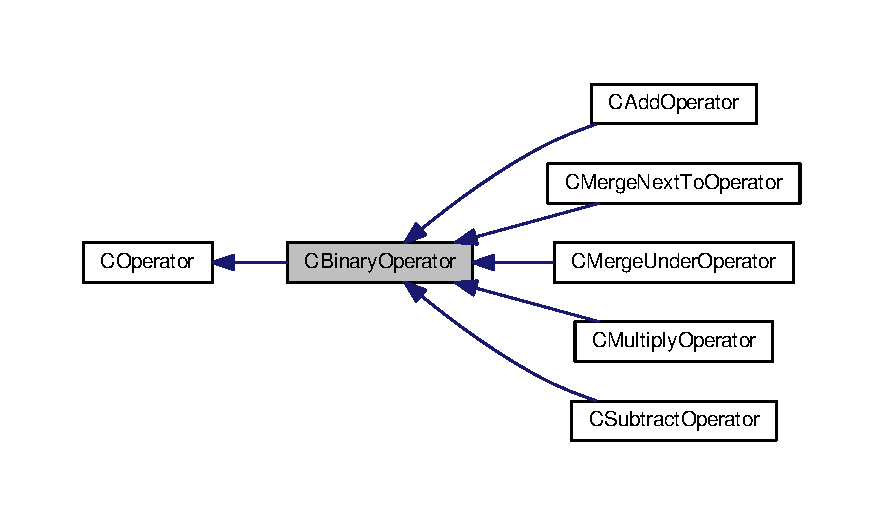
\includegraphics[width=350pt]{classCBinaryOperator__inherit__graph}
\end{center}
\end{figure}


Collaboration diagram for C\+Binary\+Operator\+:\nopagebreak
\begin{figure}[H]
\begin{center}
\leavevmode
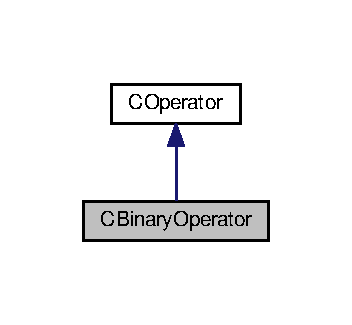
\includegraphics[width=169pt]{classCBinaryOperator__coll__graph}
\end{center}
\end{figure}
\subsection*{Public Member Functions}
\begin{DoxyCompactItemize}
\item 
\hyperlink{classCBinaryOperator_a0c0b5652ad1d96cc6922a47d7366355f}{C\+Binary\+Operator} ()=default
\item 
\hyperlink{classCBinaryOperator_a3db57fcfac0ad4c3c2b29a257bdd6fee}{C\+Binary\+Operator} (shared\+\_\+ptr$<$ \hyperlink{classCMatrix}{C\+Matrix} $>$ \&left, shared\+\_\+ptr$<$ \hyperlink{classCMatrix}{C\+Matrix} $>$ \&right)
\item 
virtual \hyperlink{classCBinaryOperator_a55459c4c7b5102ae41f77f7a1ae60e75}{$\sim$\+C\+Binary\+Operator} ()=default
\item 
virtual \hyperlink{classCMatrix}{C\+Matrix} $\ast$ \hyperlink{classCBinaryOperator_aea1eef33f83a4e395091daa0637f4c77}{Evaluate} (\hyperlink{classCMemory}{C\+Memory} \&memory)=0
\end{DoxyCompactItemize}
\subsection*{Protected Attributes}
\begin{DoxyCompactItemize}
\item 
shared\+\_\+ptr$<$ \hyperlink{classCMatrix}{C\+Matrix} $>$ \hyperlink{classCBinaryOperator_a05f24960fb48975c94b462da76aa9ad0}{m\+\_\+\+Left}
\item 
shared\+\_\+ptr$<$ \hyperlink{classCMatrix}{C\+Matrix} $>$ \hyperlink{classCBinaryOperator_a5588bc0fa7e3ca62ef3dbdb23d96f920}{m\+\_\+\+Right}
\end{DoxyCompactItemize}


\subsection{Constructor \& Destructor Documentation}
\index{C\+Binary\+Operator@{C\+Binary\+Operator}!C\+Binary\+Operator@{C\+Binary\+Operator}}
\index{C\+Binary\+Operator@{C\+Binary\+Operator}!C\+Binary\+Operator@{C\+Binary\+Operator}}
\subsubsection[{\texorpdfstring{C\+Binary\+Operator()=default}{CBinaryOperator()=default}}]{\setlength{\rightskip}{0pt plus 5cm}C\+Binary\+Operator\+::\+C\+Binary\+Operator (
\begin{DoxyParamCaption}
{}
\end{DoxyParamCaption}
)\hspace{0.3cm}{\ttfamily [default]}}\hypertarget{classCBinaryOperator_a0c0b5652ad1d96cc6922a47d7366355f}{}\label{classCBinaryOperator_a0c0b5652ad1d96cc6922a47d7366355f}
\index{C\+Binary\+Operator@{C\+Binary\+Operator}!C\+Binary\+Operator@{C\+Binary\+Operator}}
\index{C\+Binary\+Operator@{C\+Binary\+Operator}!C\+Binary\+Operator@{C\+Binary\+Operator}}
\subsubsection[{\texorpdfstring{C\+Binary\+Operator(shared\+\_\+ptr$<$ C\+Matrix $>$ \&left, shared\+\_\+ptr$<$ C\+Matrix $>$ \&right)}{CBinaryOperator(shared_ptr< CMatrix > &left, shared_ptr< CMatrix > &right)}}]{\setlength{\rightskip}{0pt plus 5cm}C\+Binary\+Operator\+::\+C\+Binary\+Operator (
\begin{DoxyParamCaption}
\item[{shared\+\_\+ptr$<$ {\bf C\+Matrix} $>$ \&}]{left, }
\item[{shared\+\_\+ptr$<$ {\bf C\+Matrix} $>$ \&}]{right}
\end{DoxyParamCaption}
)\hspace{0.3cm}{\ttfamily [inline]}}\hypertarget{classCBinaryOperator_a3db57fcfac0ad4c3c2b29a257bdd6fee}{}\label{classCBinaryOperator_a3db57fcfac0ad4c3c2b29a257bdd6fee}
\index{C\+Binary\+Operator@{C\+Binary\+Operator}!````~C\+Binary\+Operator@{$\sim$\+C\+Binary\+Operator}}
\index{````~C\+Binary\+Operator@{$\sim$\+C\+Binary\+Operator}!C\+Binary\+Operator@{C\+Binary\+Operator}}
\subsubsection[{\texorpdfstring{$\sim$\+C\+Binary\+Operator()=default}{~CBinaryOperator()=default}}]{\setlength{\rightskip}{0pt plus 5cm}virtual C\+Binary\+Operator\+::$\sim$\+C\+Binary\+Operator (
\begin{DoxyParamCaption}
{}
\end{DoxyParamCaption}
)\hspace{0.3cm}{\ttfamily [virtual]}, {\ttfamily [default]}}\hypertarget{classCBinaryOperator_a55459c4c7b5102ae41f77f7a1ae60e75}{}\label{classCBinaryOperator_a55459c4c7b5102ae41f77f7a1ae60e75}


\subsection{Member Function Documentation}
\index{C\+Binary\+Operator@{C\+Binary\+Operator}!Evaluate@{Evaluate}}
\index{Evaluate@{Evaluate}!C\+Binary\+Operator@{C\+Binary\+Operator}}
\subsubsection[{\texorpdfstring{Evaluate(\+C\+Memory \&memory)=0}{Evaluate(CMemory &memory)=0}}]{\setlength{\rightskip}{0pt plus 5cm}virtual {\bf C\+Matrix}$\ast$ C\+Binary\+Operator\+::\+Evaluate (
\begin{DoxyParamCaption}
\item[{{\bf C\+Memory} \&}]{memory}
\end{DoxyParamCaption}
)\hspace{0.3cm}{\ttfamily [pure virtual]}}\hypertarget{classCBinaryOperator_aea1eef33f83a4e395091daa0637f4c77}{}\label{classCBinaryOperator_aea1eef33f83a4e395091daa0637f4c77}


Implements \hyperlink{classCOperator_a45c8237c879a44f839247badefe6eade}{C\+Operator}.



Implemented in \hyperlink{classCAddOperator_a7fb8e83b7c5831e3f2e6e8544af49523}{C\+Add\+Operator}, \hyperlink{classCMergeNextToOperator_ab914c0ae204819b6f5e9d9857acd1854}{C\+Merge\+Next\+To\+Operator}, \hyperlink{classCMergeUnderOperator_a4b17a385b3f261bd9a5ab3cb4403e9fb}{C\+Merge\+Under\+Operator}, \hyperlink{classCMultiplyOperator_a328c99de6116b51ef3aa52705a748a85}{C\+Multiply\+Operator}, and \hyperlink{classCSubtractOperator_a09c75b8486a0056f82dcec6a5f9fcc58}{C\+Subtract\+Operator}.



\subsection{Member Data Documentation}
\index{C\+Binary\+Operator@{C\+Binary\+Operator}!m\+\_\+\+Left@{m\+\_\+\+Left}}
\index{m\+\_\+\+Left@{m\+\_\+\+Left}!C\+Binary\+Operator@{C\+Binary\+Operator}}
\subsubsection[{\texorpdfstring{m\+\_\+\+Left}{m_Left}}]{\setlength{\rightskip}{0pt plus 5cm}shared\+\_\+ptr$<${\bf C\+Matrix}$>$ C\+Binary\+Operator\+::m\+\_\+\+Left\hspace{0.3cm}{\ttfamily [protected]}}\hypertarget{classCBinaryOperator_a05f24960fb48975c94b462da76aa9ad0}{}\label{classCBinaryOperator_a05f24960fb48975c94b462da76aa9ad0}
\index{C\+Binary\+Operator@{C\+Binary\+Operator}!m\+\_\+\+Right@{m\+\_\+\+Right}}
\index{m\+\_\+\+Right@{m\+\_\+\+Right}!C\+Binary\+Operator@{C\+Binary\+Operator}}
\subsubsection[{\texorpdfstring{m\+\_\+\+Right}{m_Right}}]{\setlength{\rightskip}{0pt plus 5cm}shared\+\_\+ptr$<${\bf C\+Matrix}$>$ C\+Binary\+Operator\+::m\+\_\+\+Right\hspace{0.3cm}{\ttfamily [protected]}}\hypertarget{classCBinaryOperator_a5588bc0fa7e3ca62ef3dbdb23d96f920}{}\label{classCBinaryOperator_a5588bc0fa7e3ca62ef3dbdb23d96f920}


The documentation for this class was generated from the following file\+:\begin{DoxyCompactItemize}
\item 
src/\hyperlink{CBinaryOperator_8h}{C\+Binary\+Operator.\+h}\end{DoxyCompactItemize}

\hypertarget{classCCommand}{}\section{C\+Command Class Reference}
\label{classCCommand}\index{C\+Command@{C\+Command}}


{\ttfamily \#include $<$C\+Command.\+h$>$}



Inheritance diagram for C\+Command\+:\nopagebreak
\begin{figure}[H]
\begin{center}
\leavevmode
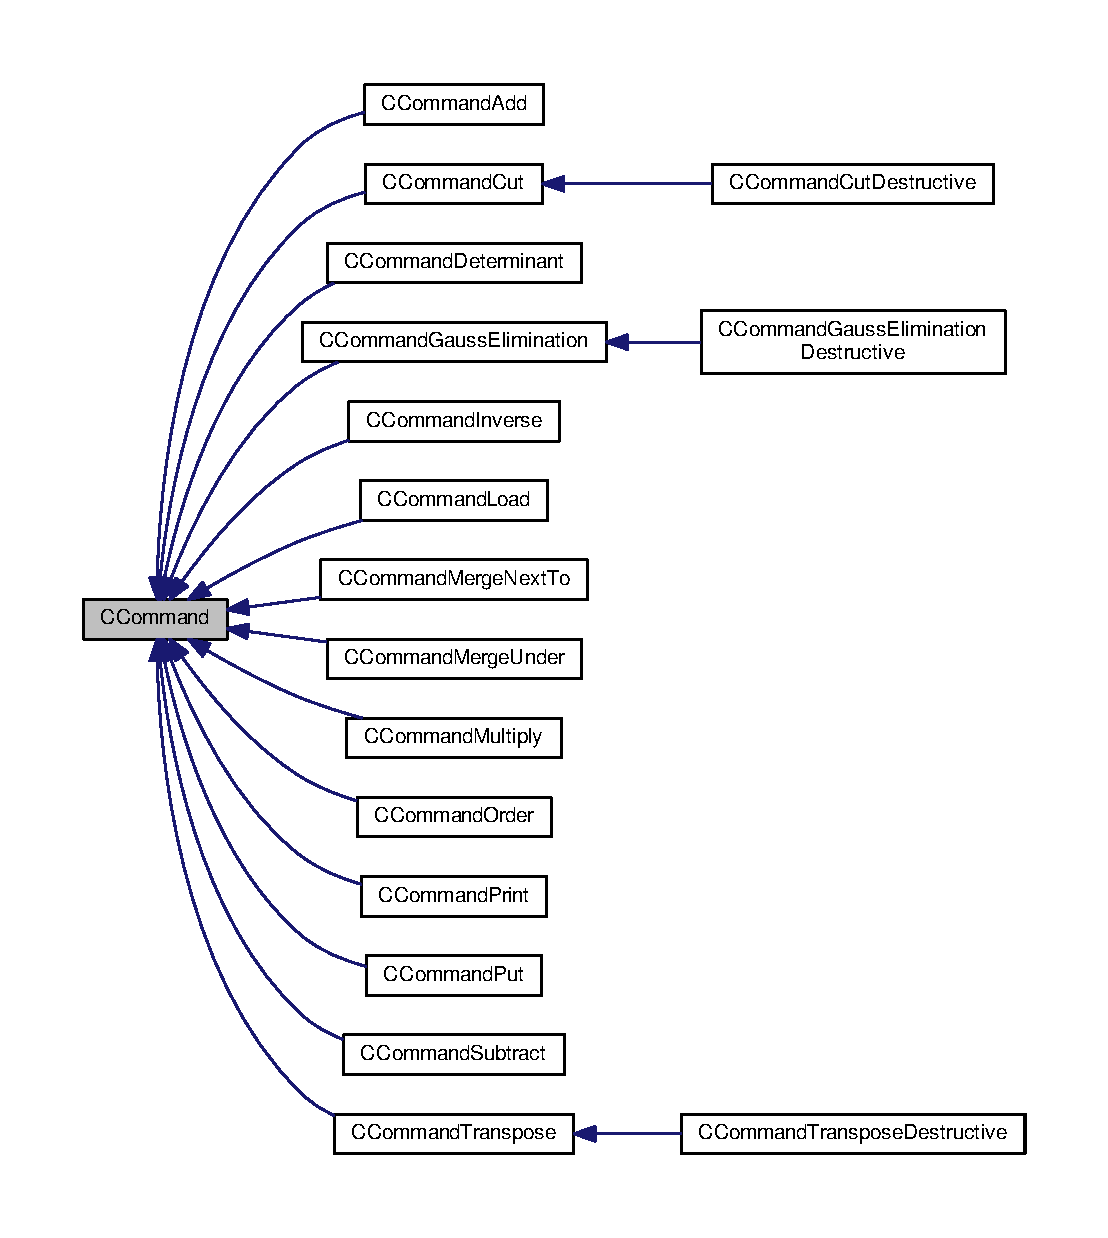
\includegraphics[height=550pt]{classCCommand__inherit__graph}
\end{center}
\end{figure}
\subsection*{Public Member Functions}
\begin{DoxyCompactItemize}
\item 
\hyperlink{classCCommand_af50175d5481d07679cf015fedff6afa7}{C\+Command} ()=default
\item 
virtual bool \hyperlink{classCCommand_ad9361ea814093c4ebecf22bb0a3f8b79}{Execute} (\hyperlink{classCMemory}{C\+Memory} \&memory)=0
\item 
virtual \hyperlink{classCCommand_a8b2c385d38a996872c963fcff08b3809}{$\sim$\+C\+Command} ()=default
\end{DoxyCompactItemize}
\subsection*{Public Attributes}
\begin{DoxyCompactItemize}
\item 
string \hyperlink{classCCommand_a95d58d40a428b703b727d8f847e6de1e}{m\+\_\+\+Result}
\item 
unique\+\_\+ptr$<$ \hyperlink{classCMatrix}{C\+Matrix} $>$ \hyperlink{classCCommand_a5192105298cdb9ea3ef5c3d3aaeba50e}{m\+\_\+\+Result\+Matrix}
\end{DoxyCompactItemize}


\subsection{Constructor \& Destructor Documentation}
\index{C\+Command@{C\+Command}!C\+Command@{C\+Command}}
\index{C\+Command@{C\+Command}!C\+Command@{C\+Command}}
\subsubsection[{\texorpdfstring{C\+Command()=default}{CCommand()=default}}]{\setlength{\rightskip}{0pt plus 5cm}C\+Command\+::\+C\+Command (
\begin{DoxyParamCaption}
{}
\end{DoxyParamCaption}
)\hspace{0.3cm}{\ttfamily [default]}}\hypertarget{classCCommand_af50175d5481d07679cf015fedff6afa7}{}\label{classCCommand_af50175d5481d07679cf015fedff6afa7}
\index{C\+Command@{C\+Command}!````~C\+Command@{$\sim$\+C\+Command}}
\index{````~C\+Command@{$\sim$\+C\+Command}!C\+Command@{C\+Command}}
\subsubsection[{\texorpdfstring{$\sim$\+C\+Command()=default}{~CCommand()=default}}]{\setlength{\rightskip}{0pt plus 5cm}virtual C\+Command\+::$\sim$\+C\+Command (
\begin{DoxyParamCaption}
{}
\end{DoxyParamCaption}
)\hspace{0.3cm}{\ttfamily [virtual]}, {\ttfamily [default]}}\hypertarget{classCCommand_a8b2c385d38a996872c963fcff08b3809}{}\label{classCCommand_a8b2c385d38a996872c963fcff08b3809}


\subsection{Member Function Documentation}
\index{C\+Command@{C\+Command}!Execute@{Execute}}
\index{Execute@{Execute}!C\+Command@{C\+Command}}
\subsubsection[{\texorpdfstring{Execute(\+C\+Memory \&memory)=0}{Execute(CMemory &memory)=0}}]{\setlength{\rightskip}{0pt plus 5cm}virtual bool C\+Command\+::\+Execute (
\begin{DoxyParamCaption}
\item[{{\bf C\+Memory} \&}]{memory}
\end{DoxyParamCaption}
)\hspace{0.3cm}{\ttfamily [pure virtual]}}\hypertarget{classCCommand_ad9361ea814093c4ebecf22bb0a3f8b79}{}\label{classCCommand_ad9361ea814093c4ebecf22bb0a3f8b79}


Implemented in \hyperlink{classCCommandLoad_a5940ee064de6b5497e9b868b1add9880}{C\+Command\+Load}, \hyperlink{classCCommandCut_a18065504c797f4fde787a7dfd46bce74}{C\+Command\+Cut}, \hyperlink{classCCommandAdd_a1280a1d17ef3465668a7de11fa712554}{C\+Command\+Add}, \hyperlink{classCCommandInverse_aa579b94f10fa18b4759fd2986629f7db}{C\+Command\+Inverse}, \hyperlink{classCCommandPut_a4b82c56cf3d5aafc75701ec72f8f17dc}{C\+Command\+Put}, \hyperlink{classCCommandSubtract_ade3f2032aab4edce747d251e89a6398b}{C\+Command\+Subtract}, \hyperlink{classCCommandMergeNextTo_acca1ef026b0bad3d44f1e4ba09276361}{C\+Command\+Merge\+Next\+To}, \hyperlink{classCCommandMergeUnder_abf1fb6fe63188e0ba0dc82dfa7bac083}{C\+Command\+Merge\+Under}, \hyperlink{classCCommandMultiply_a06d75c2d7c89607406de6c05e586907f}{C\+Command\+Multiply}, \hyperlink{classCCommandOrder_a26192670b49e62a03d8ce240c1e2c983}{C\+Command\+Order}, \hyperlink{classCCommandTranspose_aa422d6b8bbe3efb23bcc479646392238}{C\+Command\+Transpose}, \hyperlink{classCCommandDeterminant_ad472106c8565309dc1f32d2559b421ec}{C\+Command\+Determinant}, \hyperlink{classCCommandGaussElimination_a450365c81652a0963554944693c6e76c}{C\+Command\+Gauss\+Elimination}, and \hyperlink{classCCommandPrint_afa1b192d43baa81c5ea9884972366643}{C\+Command\+Print}.



\subsection{Member Data Documentation}
\index{C\+Command@{C\+Command}!m\+\_\+\+Result@{m\+\_\+\+Result}}
\index{m\+\_\+\+Result@{m\+\_\+\+Result}!C\+Command@{C\+Command}}
\subsubsection[{\texorpdfstring{m\+\_\+\+Result}{m_Result}}]{\setlength{\rightskip}{0pt plus 5cm}string C\+Command\+::m\+\_\+\+Result}\hypertarget{classCCommand_a95d58d40a428b703b727d8f847e6de1e}{}\label{classCCommand_a95d58d40a428b703b727d8f847e6de1e}
\index{C\+Command@{C\+Command}!m\+\_\+\+Result\+Matrix@{m\+\_\+\+Result\+Matrix}}
\index{m\+\_\+\+Result\+Matrix@{m\+\_\+\+Result\+Matrix}!C\+Command@{C\+Command}}
\subsubsection[{\texorpdfstring{m\+\_\+\+Result\+Matrix}{m_ResultMatrix}}]{\setlength{\rightskip}{0pt plus 5cm}unique\+\_\+ptr$<${\bf C\+Matrix}$>$ C\+Command\+::m\+\_\+\+Result\+Matrix}\hypertarget{classCCommand_a5192105298cdb9ea3ef5c3d3aaeba50e}{}\label{classCCommand_a5192105298cdb9ea3ef5c3d3aaeba50e}


The documentation for this class was generated from the following file\+:\begin{DoxyCompactItemize}
\item 
src/\hyperlink{CCommand_8h}{C\+Command.\+h}\end{DoxyCompactItemize}

\hypertarget{classCCommandAdd}{}\section{C\+Command\+Add Class Reference}
\label{classCCommandAdd}\index{C\+Command\+Add@{C\+Command\+Add}}


{\ttfamily \#include $<$C\+Command\+Add.\+h$>$}



Inheritance diagram for C\+Command\+Add\+:\nopagebreak
\begin{figure}[H]
\begin{center}
\leavevmode
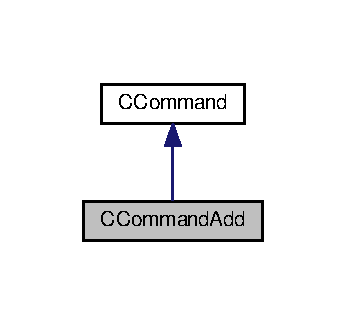
\includegraphics[width=166pt]{classCCommandAdd__inherit__graph}
\end{center}
\end{figure}


Collaboration diagram for C\+Command\+Add\+:\nopagebreak
\begin{figure}[H]
\begin{center}
\leavevmode
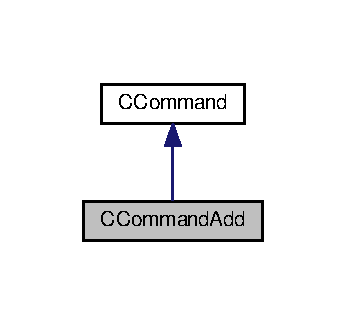
\includegraphics[width=166pt]{classCCommandAdd__coll__graph}
\end{center}
\end{figure}
\subsection*{Public Member Functions}
\begin{DoxyCompactItemize}
\item 
\hyperlink{classCCommandAdd_a41bc29d57d43751ff561d0c9092d57cd}{C\+Command\+Add} ()
\item 
\hyperlink{classCCommandAdd_af5ae9f4e2187aa9cea5c052621a2d5f6}{$\sim$\+C\+Command\+Add} () override=default
\item 
\hyperlink{classCCommandAdd_a40c2fa07a479459ed99910b87364f234}{C\+Command\+Add} (string operand1, string operand2)
\item 
bool \hyperlink{classCCommandAdd_a1280a1d17ef3465668a7de11fa712554}{Execute} (\hyperlink{classCMemory}{C\+Memory} \&memory) override
\end{DoxyCompactItemize}
\subsection*{Private Attributes}
\begin{DoxyCompactItemize}
\item 
string \hyperlink{classCCommandAdd_abcd42da999946000498850d594d2720b}{m\+\_\+\+Operand1}
\item 
string \hyperlink{classCCommandAdd_aa27354561d8bfe6e81409fbe35dfede8}{m\+\_\+\+Operand2}
\end{DoxyCompactItemize}
\subsection*{Additional Inherited Members}


\subsection{Constructor \& Destructor Documentation}
\index{C\+Command\+Add@{C\+Command\+Add}!C\+Command\+Add@{C\+Command\+Add}}
\index{C\+Command\+Add@{C\+Command\+Add}!C\+Command\+Add@{C\+Command\+Add}}
\subsubsection[{\texorpdfstring{C\+Command\+Add()}{CCommandAdd()}}]{\setlength{\rightskip}{0pt plus 5cm}C\+Command\+Add\+::\+C\+Command\+Add (
\begin{DoxyParamCaption}
{}
\end{DoxyParamCaption}
)\hspace{0.3cm}{\ttfamily [inline]}}\hypertarget{classCCommandAdd_a41bc29d57d43751ff561d0c9092d57cd}{}\label{classCCommandAdd_a41bc29d57d43751ff561d0c9092d57cd}
\index{C\+Command\+Add@{C\+Command\+Add}!````~C\+Command\+Add@{$\sim$\+C\+Command\+Add}}
\index{````~C\+Command\+Add@{$\sim$\+C\+Command\+Add}!C\+Command\+Add@{C\+Command\+Add}}
\subsubsection[{\texorpdfstring{$\sim$\+C\+Command\+Add() override=default}{~CCommandAdd() override=default}}]{\setlength{\rightskip}{0pt plus 5cm}C\+Command\+Add\+::$\sim$\+C\+Command\+Add (
\begin{DoxyParamCaption}
{}
\end{DoxyParamCaption}
)\hspace{0.3cm}{\ttfamily [override]}, {\ttfamily [default]}}\hypertarget{classCCommandAdd_af5ae9f4e2187aa9cea5c052621a2d5f6}{}\label{classCCommandAdd_af5ae9f4e2187aa9cea5c052621a2d5f6}
\index{C\+Command\+Add@{C\+Command\+Add}!C\+Command\+Add@{C\+Command\+Add}}
\index{C\+Command\+Add@{C\+Command\+Add}!C\+Command\+Add@{C\+Command\+Add}}
\subsubsection[{\texorpdfstring{C\+Command\+Add(string operand1, string operand2)}{CCommandAdd(string operand1, string operand2)}}]{\setlength{\rightskip}{0pt plus 5cm}C\+Command\+Add\+::\+C\+Command\+Add (
\begin{DoxyParamCaption}
\item[{string}]{operand1, }
\item[{string}]{operand2}
\end{DoxyParamCaption}
)\hspace{0.3cm}{\ttfamily [inline]}}\hypertarget{classCCommandAdd_a40c2fa07a479459ed99910b87364f234}{}\label{classCCommandAdd_a40c2fa07a479459ed99910b87364f234}


\subsection{Member Function Documentation}
\index{C\+Command\+Add@{C\+Command\+Add}!Execute@{Execute}}
\index{Execute@{Execute}!C\+Command\+Add@{C\+Command\+Add}}
\subsubsection[{\texorpdfstring{Execute(\+C\+Memory \&memory) override}{Execute(CMemory &memory) override}}]{\setlength{\rightskip}{0pt plus 5cm}bool C\+Command\+Add\+::\+Execute (
\begin{DoxyParamCaption}
\item[{{\bf C\+Memory} \&}]{memory}
\end{DoxyParamCaption}
)\hspace{0.3cm}{\ttfamily [override]}, {\ttfamily [virtual]}}\hypertarget{classCCommandAdd_a1280a1d17ef3465668a7de11fa712554}{}\label{classCCommandAdd_a1280a1d17ef3465668a7de11fa712554}
Execute command. 
\begin{DoxyParams}{Parameters}
{\em memory} & \\
\hline
\end{DoxyParams}
\begin{DoxyReturn}{Returns}
true if execution successful, false otherwise (command cannot be performed) 
\end{DoxyReturn}


Implements \hyperlink{classCCommand_ad9361ea814093c4ebecf22bb0a3f8b79}{C\+Command}.



\subsection{Member Data Documentation}
\index{C\+Command\+Add@{C\+Command\+Add}!m\+\_\+\+Operand1@{m\+\_\+\+Operand1}}
\index{m\+\_\+\+Operand1@{m\+\_\+\+Operand1}!C\+Command\+Add@{C\+Command\+Add}}
\subsubsection[{\texorpdfstring{m\+\_\+\+Operand1}{m_Operand1}}]{\setlength{\rightskip}{0pt plus 5cm}string C\+Command\+Add\+::m\+\_\+\+Operand1\hspace{0.3cm}{\ttfamily [private]}}\hypertarget{classCCommandAdd_abcd42da999946000498850d594d2720b}{}\label{classCCommandAdd_abcd42da999946000498850d594d2720b}
\index{C\+Command\+Add@{C\+Command\+Add}!m\+\_\+\+Operand2@{m\+\_\+\+Operand2}}
\index{m\+\_\+\+Operand2@{m\+\_\+\+Operand2}!C\+Command\+Add@{C\+Command\+Add}}
\subsubsection[{\texorpdfstring{m\+\_\+\+Operand2}{m_Operand2}}]{\setlength{\rightskip}{0pt plus 5cm}string C\+Command\+Add\+::m\+\_\+\+Operand2\hspace{0.3cm}{\ttfamily [private]}}\hypertarget{classCCommandAdd_aa27354561d8bfe6e81409fbe35dfede8}{}\label{classCCommandAdd_aa27354561d8bfe6e81409fbe35dfede8}


The documentation for this class was generated from the following files\+:\begin{DoxyCompactItemize}
\item 
src/\hyperlink{CCommandAdd_8h}{C\+Command\+Add.\+h}\item 
src/\hyperlink{CCommandAdd_8cpp}{C\+Command\+Add.\+cpp}\end{DoxyCompactItemize}

\hypertarget{classCCommandCut}{}\section{C\+Command\+Cut Class Reference}
\label{classCCommandCut}\index{C\+Command\+Cut@{C\+Command\+Cut}}


{\ttfamily \#include $<$C\+Command\+Cut.\+h$>$}



Inheritance diagram for C\+Command\+Cut\+:\nopagebreak
\begin{figure}[H]
\begin{center}
\leavevmode
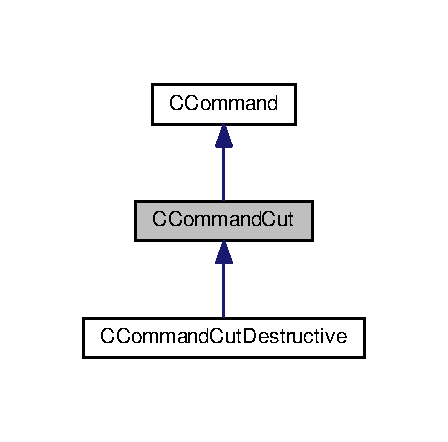
\includegraphics[width=215pt]{classCCommandCut__inherit__graph}
\end{center}
\end{figure}


Collaboration diagram for C\+Command\+Cut\+:\nopagebreak
\begin{figure}[H]
\begin{center}
\leavevmode
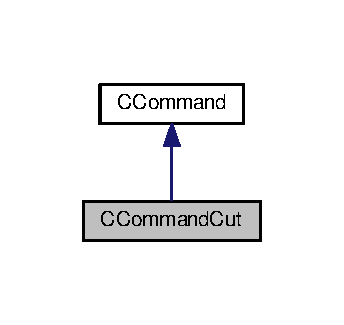
\includegraphics[width=165pt]{classCCommandCut__coll__graph}
\end{center}
\end{figure}
\subsection*{Public Member Functions}
\begin{DoxyCompactItemize}
\item 
\hyperlink{classCCommandCut_aea6d6e3ee2b71412f0cd7d28ddf716a5}{C\+Command\+Cut} ()
\item 
\hyperlink{classCCommandCut_aa4c585b4f9fe99f10a39014329f02614}{$\sim$\+C\+Command\+Cut} () override=default
\item 
\hyperlink{classCCommandCut_adf50105fd0734790ab29a3bf1edfcd4e}{C\+Command\+Cut} (string var\+Name, std\+::size\+\_\+t num\+Rows, size\+\_\+t num\+Cols, pair$<$ std\+::size\+\_\+t, std\+::size\+\_\+t $>$ start\+Point)
\item 
bool \hyperlink{classCCommandCut_a18065504c797f4fde787a7dfd46bce74}{Execute} (\hyperlink{classCMemory}{C\+Memory} \&memory) override
\end{DoxyCompactItemize}
\subsection*{Protected Attributes}
\begin{DoxyCompactItemize}
\item 
string \hyperlink{classCCommandCut_aeb69b9b4f3e1c319de83c2753294e2db}{m\+\_\+\+Var\+Name}
\item 
std\+::size\+\_\+t \hyperlink{classCCommandCut_ae1021a795aa0ca34697021ed9c68ea33}{m\+\_\+\+Num\+Rows} \{\}
\item 
std\+::size\+\_\+t \hyperlink{classCCommandCut_a0073be24f9b9bfdb3a4194bd4ea16bbc}{m\+\_\+\+Num\+Cols} \{\}
\item 
pair$<$ std\+::size\+\_\+t, size\+\_\+t $>$ \hyperlink{classCCommandCut_adbd994d2b9e2620042427235516b446b}{m\+\_\+\+Start\+Point}
\end{DoxyCompactItemize}
\subsection*{Additional Inherited Members}


\subsection{Constructor \& Destructor Documentation}
\index{C\+Command\+Cut@{C\+Command\+Cut}!C\+Command\+Cut@{C\+Command\+Cut}}
\index{C\+Command\+Cut@{C\+Command\+Cut}!C\+Command\+Cut@{C\+Command\+Cut}}
\subsubsection[{\texorpdfstring{C\+Command\+Cut()}{CCommandCut()}}]{\setlength{\rightskip}{0pt plus 5cm}C\+Command\+Cut\+::\+C\+Command\+Cut (
\begin{DoxyParamCaption}
{}
\end{DoxyParamCaption}
)\hspace{0.3cm}{\ttfamily [inline]}}\hypertarget{classCCommandCut_aea6d6e3ee2b71412f0cd7d28ddf716a5}{}\label{classCCommandCut_aea6d6e3ee2b71412f0cd7d28ddf716a5}
\index{C\+Command\+Cut@{C\+Command\+Cut}!````~C\+Command\+Cut@{$\sim$\+C\+Command\+Cut}}
\index{````~C\+Command\+Cut@{$\sim$\+C\+Command\+Cut}!C\+Command\+Cut@{C\+Command\+Cut}}
\subsubsection[{\texorpdfstring{$\sim$\+C\+Command\+Cut() override=default}{~CCommandCut() override=default}}]{\setlength{\rightskip}{0pt plus 5cm}C\+Command\+Cut\+::$\sim$\+C\+Command\+Cut (
\begin{DoxyParamCaption}
{}
\end{DoxyParamCaption}
)\hspace{0.3cm}{\ttfamily [override]}, {\ttfamily [default]}}\hypertarget{classCCommandCut_aa4c585b4f9fe99f10a39014329f02614}{}\label{classCCommandCut_aa4c585b4f9fe99f10a39014329f02614}
\index{C\+Command\+Cut@{C\+Command\+Cut}!C\+Command\+Cut@{C\+Command\+Cut}}
\index{C\+Command\+Cut@{C\+Command\+Cut}!C\+Command\+Cut@{C\+Command\+Cut}}
\subsubsection[{\texorpdfstring{C\+Command\+Cut(string var\+Name, std\+::size\+\_\+t num\+Rows, size\+\_\+t num\+Cols, pair$<$ std\+::size\+\_\+t, std\+::size\+\_\+t $>$ start\+Point)}{CCommandCut(string varName, std::size_t numRows, size_t numCols, pair< std::size_t, std::size_t > startPoint)}}]{\setlength{\rightskip}{0pt plus 5cm}C\+Command\+Cut\+::\+C\+Command\+Cut (
\begin{DoxyParamCaption}
\item[{string}]{var\+Name, }
\item[{std\+::size\+\_\+t}]{num\+Rows, }
\item[{size\+\_\+t}]{num\+Cols, }
\item[{pair$<$ std\+::size\+\_\+t, std\+::size\+\_\+t $>$}]{start\+Point}
\end{DoxyParamCaption}
)\hspace{0.3cm}{\ttfamily [inline]}}\hypertarget{classCCommandCut_adf50105fd0734790ab29a3bf1edfcd4e}{}\label{classCCommandCut_adf50105fd0734790ab29a3bf1edfcd4e}


\subsection{Member Function Documentation}
\index{C\+Command\+Cut@{C\+Command\+Cut}!Execute@{Execute}}
\index{Execute@{Execute}!C\+Command\+Cut@{C\+Command\+Cut}}
\subsubsection[{\texorpdfstring{Execute(\+C\+Memory \&memory) override}{Execute(CMemory &memory) override}}]{\setlength{\rightskip}{0pt plus 5cm}bool C\+Command\+Cut\+::\+Execute (
\begin{DoxyParamCaption}
\item[{{\bf C\+Memory} \&}]{memory}
\end{DoxyParamCaption}
)\hspace{0.3cm}{\ttfamily [override]}, {\ttfamily [virtual]}}\hypertarget{classCCommandCut_a18065504c797f4fde787a7dfd46bce74}{}\label{classCCommandCut_a18065504c797f4fde787a7dfd46bce74}
Execute command. 
\begin{DoxyParams}{Parameters}
{\em memory} & \\
\hline
\end{DoxyParams}
\begin{DoxyReturn}{Returns}
true if execution successful, false otherwise (command cannot be performed) 
\end{DoxyReturn}


Implements \hyperlink{classCCommand_ad9361ea814093c4ebecf22bb0a3f8b79}{C\+Command}.



Reimplemented in \hyperlink{classCCommandCutDestructive_a6c5d4d6753bcb5c480e26b880c863da1}{C\+Command\+Cut\+Destructive}.



\subsection{Member Data Documentation}
\index{C\+Command\+Cut@{C\+Command\+Cut}!m\+\_\+\+Num\+Cols@{m\+\_\+\+Num\+Cols}}
\index{m\+\_\+\+Num\+Cols@{m\+\_\+\+Num\+Cols}!C\+Command\+Cut@{C\+Command\+Cut}}
\subsubsection[{\texorpdfstring{m\+\_\+\+Num\+Cols}{m_NumCols}}]{\setlength{\rightskip}{0pt plus 5cm}std\+::size\+\_\+t C\+Command\+Cut\+::m\+\_\+\+Num\+Cols \{\}\hspace{0.3cm}{\ttfamily [protected]}}\hypertarget{classCCommandCut_a0073be24f9b9bfdb3a4194bd4ea16bbc}{}\label{classCCommandCut_a0073be24f9b9bfdb3a4194bd4ea16bbc}
\index{C\+Command\+Cut@{C\+Command\+Cut}!m\+\_\+\+Num\+Rows@{m\+\_\+\+Num\+Rows}}
\index{m\+\_\+\+Num\+Rows@{m\+\_\+\+Num\+Rows}!C\+Command\+Cut@{C\+Command\+Cut}}
\subsubsection[{\texorpdfstring{m\+\_\+\+Num\+Rows}{m_NumRows}}]{\setlength{\rightskip}{0pt plus 5cm}std\+::size\+\_\+t C\+Command\+Cut\+::m\+\_\+\+Num\+Rows \{\}\hspace{0.3cm}{\ttfamily [protected]}}\hypertarget{classCCommandCut_ae1021a795aa0ca34697021ed9c68ea33}{}\label{classCCommandCut_ae1021a795aa0ca34697021ed9c68ea33}
\index{C\+Command\+Cut@{C\+Command\+Cut}!m\+\_\+\+Start\+Point@{m\+\_\+\+Start\+Point}}
\index{m\+\_\+\+Start\+Point@{m\+\_\+\+Start\+Point}!C\+Command\+Cut@{C\+Command\+Cut}}
\subsubsection[{\texorpdfstring{m\+\_\+\+Start\+Point}{m_StartPoint}}]{\setlength{\rightskip}{0pt plus 5cm}pair$<$std\+::size\+\_\+t, size\+\_\+t$>$ C\+Command\+Cut\+::m\+\_\+\+Start\+Point\hspace{0.3cm}{\ttfamily [protected]}}\hypertarget{classCCommandCut_adbd994d2b9e2620042427235516b446b}{}\label{classCCommandCut_adbd994d2b9e2620042427235516b446b}
\index{C\+Command\+Cut@{C\+Command\+Cut}!m\+\_\+\+Var\+Name@{m\+\_\+\+Var\+Name}}
\index{m\+\_\+\+Var\+Name@{m\+\_\+\+Var\+Name}!C\+Command\+Cut@{C\+Command\+Cut}}
\subsubsection[{\texorpdfstring{m\+\_\+\+Var\+Name}{m_VarName}}]{\setlength{\rightskip}{0pt plus 5cm}string C\+Command\+Cut\+::m\+\_\+\+Var\+Name\hspace{0.3cm}{\ttfamily [protected]}}\hypertarget{classCCommandCut_aeb69b9b4f3e1c319de83c2753294e2db}{}\label{classCCommandCut_aeb69b9b4f3e1c319de83c2753294e2db}


The documentation for this class was generated from the following files\+:\begin{DoxyCompactItemize}
\item 
src/\hyperlink{CCommandCut_8h}{C\+Command\+Cut.\+h}\item 
src/\hyperlink{CCommandCut_8cpp}{C\+Command\+Cut.\+cpp}\end{DoxyCompactItemize}

\hypertarget{classCCommandDeterminant}{}\section{C\+Command\+Determinant Class Reference}
\label{classCCommandDeterminant}\index{C\+Command\+Determinant@{C\+Command\+Determinant}}


{\ttfamily \#include $<$C\+Command\+Determinant.\+h$>$}



Inheritance diagram for C\+Command\+Determinant\+:\nopagebreak
\begin{figure}[H]
\begin{center}
\leavevmode
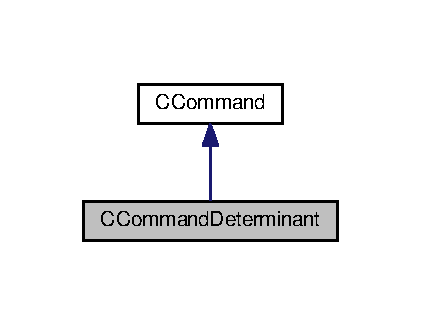
\includegraphics[width=202pt]{classCCommandDeterminant__inherit__graph}
\end{center}
\end{figure}


Collaboration diagram for C\+Command\+Determinant\+:\nopagebreak
\begin{figure}[H]
\begin{center}
\leavevmode
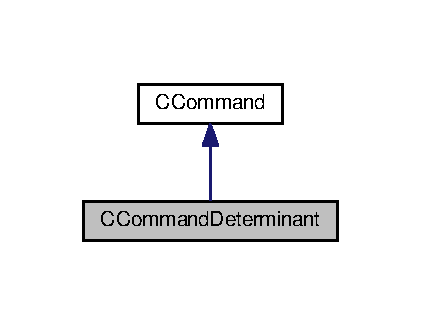
\includegraphics[width=202pt]{classCCommandDeterminant__coll__graph}
\end{center}
\end{figure}
\subsection*{Public Member Functions}
\begin{DoxyCompactItemize}
\item 
\hyperlink{classCCommandDeterminant_a040acf83a2a792f5bdc8e84d4d7ea986}{C\+Command\+Determinant} ()
\item 
\hyperlink{classCCommandDeterminant_ae9ac7cf4568af2805d18ddb65824635b}{$\sim$\+C\+Command\+Determinant} () override=default
\item 
\hyperlink{classCCommandDeterminant_a193c274c4ba951b425bf390347fa7d59}{C\+Command\+Determinant} (string var\+Name)
\item 
bool \hyperlink{classCCommandDeterminant_ad472106c8565309dc1f32d2559b421ec}{Execute} (\hyperlink{classCMemory}{C\+Memory} \&memory) override
\end{DoxyCompactItemize}
\subsection*{Public Attributes}
\begin{DoxyCompactItemize}
\item 
double \hyperlink{classCCommandDeterminant_a4a8778e30170613ead5997c7b18438c8}{m\+\_\+\+Determinant}
\end{DoxyCompactItemize}
\subsection*{Private Attributes}
\begin{DoxyCompactItemize}
\item 
string \hyperlink{classCCommandDeterminant_aa5df4a490c14743c5d6a4e65df406bc3}{m\+\_\+\+Var\+Name}
\end{DoxyCompactItemize}


\subsection{Constructor \& Destructor Documentation}
\index{C\+Command\+Determinant@{C\+Command\+Determinant}!C\+Command\+Determinant@{C\+Command\+Determinant}}
\index{C\+Command\+Determinant@{C\+Command\+Determinant}!C\+Command\+Determinant@{C\+Command\+Determinant}}
\subsubsection[{\texorpdfstring{C\+Command\+Determinant()}{CCommandDeterminant()}}]{\setlength{\rightskip}{0pt plus 5cm}C\+Command\+Determinant\+::\+C\+Command\+Determinant (
\begin{DoxyParamCaption}
{}
\end{DoxyParamCaption}
)\hspace{0.3cm}{\ttfamily [inline]}}\hypertarget{classCCommandDeterminant_a040acf83a2a792f5bdc8e84d4d7ea986}{}\label{classCCommandDeterminant_a040acf83a2a792f5bdc8e84d4d7ea986}
\index{C\+Command\+Determinant@{C\+Command\+Determinant}!````~C\+Command\+Determinant@{$\sim$\+C\+Command\+Determinant}}
\index{````~C\+Command\+Determinant@{$\sim$\+C\+Command\+Determinant}!C\+Command\+Determinant@{C\+Command\+Determinant}}
\subsubsection[{\texorpdfstring{$\sim$\+C\+Command\+Determinant() override=default}{~CCommandDeterminant() override=default}}]{\setlength{\rightskip}{0pt plus 5cm}C\+Command\+Determinant\+::$\sim$\+C\+Command\+Determinant (
\begin{DoxyParamCaption}
{}
\end{DoxyParamCaption}
)\hspace{0.3cm}{\ttfamily [override]}, {\ttfamily [default]}}\hypertarget{classCCommandDeterminant_ae9ac7cf4568af2805d18ddb65824635b}{}\label{classCCommandDeterminant_ae9ac7cf4568af2805d18ddb65824635b}
\index{C\+Command\+Determinant@{C\+Command\+Determinant}!C\+Command\+Determinant@{C\+Command\+Determinant}}
\index{C\+Command\+Determinant@{C\+Command\+Determinant}!C\+Command\+Determinant@{C\+Command\+Determinant}}
\subsubsection[{\texorpdfstring{C\+Command\+Determinant(string var\+Name)}{CCommandDeterminant(string varName)}}]{\setlength{\rightskip}{0pt plus 5cm}C\+Command\+Determinant\+::\+C\+Command\+Determinant (
\begin{DoxyParamCaption}
\item[{string}]{var\+Name}
\end{DoxyParamCaption}
)\hspace{0.3cm}{\ttfamily [inline]}}\hypertarget{classCCommandDeterminant_a193c274c4ba951b425bf390347fa7d59}{}\label{classCCommandDeterminant_a193c274c4ba951b425bf390347fa7d59}


\subsection{Member Function Documentation}
\index{C\+Command\+Determinant@{C\+Command\+Determinant}!Execute@{Execute}}
\index{Execute@{Execute}!C\+Command\+Determinant@{C\+Command\+Determinant}}
\subsubsection[{\texorpdfstring{Execute(\+C\+Memory \&memory) override}{Execute(CMemory &memory) override}}]{\setlength{\rightskip}{0pt plus 5cm}bool C\+Command\+Determinant\+::\+Execute (
\begin{DoxyParamCaption}
\item[{{\bf C\+Memory} \&}]{memory}
\end{DoxyParamCaption}
)\hspace{0.3cm}{\ttfamily [inline]}, {\ttfamily [override]}, {\ttfamily [virtual]}}\hypertarget{classCCommandDeterminant_ad472106c8565309dc1f32d2559b421ec}{}\label{classCCommandDeterminant_ad472106c8565309dc1f32d2559b421ec}


Implements \hyperlink{classCCommand_ad9361ea814093c4ebecf22bb0a3f8b79}{C\+Command}.



\subsection{Member Data Documentation}
\index{C\+Command\+Determinant@{C\+Command\+Determinant}!m\+\_\+\+Determinant@{m\+\_\+\+Determinant}}
\index{m\+\_\+\+Determinant@{m\+\_\+\+Determinant}!C\+Command\+Determinant@{C\+Command\+Determinant}}
\subsubsection[{\texorpdfstring{m\+\_\+\+Determinant}{m_Determinant}}]{\setlength{\rightskip}{0pt plus 5cm}double C\+Command\+Determinant\+::m\+\_\+\+Determinant}\hypertarget{classCCommandDeterminant_a4a8778e30170613ead5997c7b18438c8}{}\label{classCCommandDeterminant_a4a8778e30170613ead5997c7b18438c8}
\index{C\+Command\+Determinant@{C\+Command\+Determinant}!m\+\_\+\+Var\+Name@{m\+\_\+\+Var\+Name}}
\index{m\+\_\+\+Var\+Name@{m\+\_\+\+Var\+Name}!C\+Command\+Determinant@{C\+Command\+Determinant}}
\subsubsection[{\texorpdfstring{m\+\_\+\+Var\+Name}{m_VarName}}]{\setlength{\rightskip}{0pt plus 5cm}string C\+Command\+Determinant\+::m\+\_\+\+Var\+Name\hspace{0.3cm}{\ttfamily [private]}}\hypertarget{classCCommandDeterminant_aa5df4a490c14743c5d6a4e65df406bc3}{}\label{classCCommandDeterminant_aa5df4a490c14743c5d6a4e65df406bc3}


The documentation for this class was generated from the following file\+:\begin{DoxyCompactItemize}
\item 
src/\hyperlink{CCommandDeterminant_8h}{C\+Command\+Determinant.\+h}\end{DoxyCompactItemize}

\hypertarget{classCCommandGaussElimination}{}\section{C\+Command\+Gauss\+Elimination Class Reference}
\label{classCCommandGaussElimination}\index{C\+Command\+Gauss\+Elimination@{C\+Command\+Gauss\+Elimination}}


{\ttfamily \#include $<$C\+Command\+Gauss\+Elimination.\+h$>$}



Inheritance diagram for C\+Command\+Gauss\+Elimination\+:\nopagebreak
\begin{figure}[H]
\begin{center}
\leavevmode
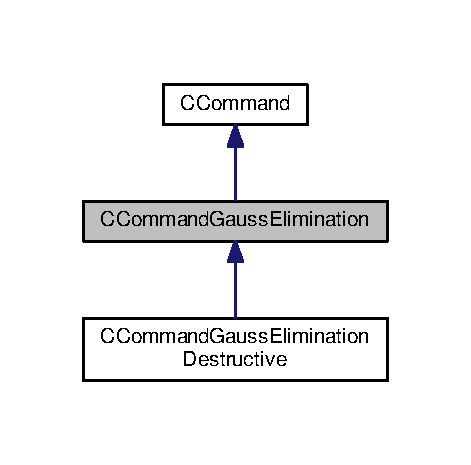
\includegraphics[width=226pt]{classCCommandGaussElimination__inherit__graph}
\end{center}
\end{figure}


Collaboration diagram for C\+Command\+Gauss\+Elimination\+:\nopagebreak
\begin{figure}[H]
\begin{center}
\leavevmode
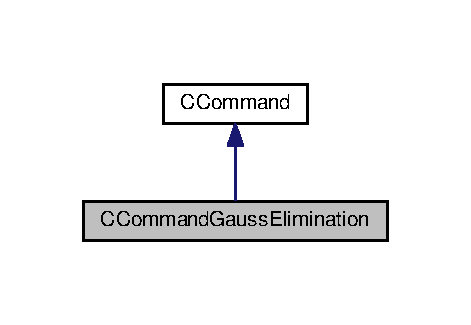
\includegraphics[width=226pt]{classCCommandGaussElimination__coll__graph}
\end{center}
\end{figure}
\subsection*{Public Member Functions}
\begin{DoxyCompactItemize}
\item 
\hyperlink{classCCommandGaussElimination_aefc96f03e386afebdadef7225bba3743}{C\+Command\+Gauss\+Elimination} ()
\item 
\hyperlink{classCCommandGaussElimination_ad694b87633ac4281f102487dcc24dd07}{$\sim$\+C\+Command\+Gauss\+Elimination} () override=default
\item 
bool \hyperlink{classCCommandGaussElimination_a450365c81652a0963554944693c6e76c}{Execute} (\hyperlink{classCMemory}{C\+Memory} \&memory) override
\item 
\hyperlink{classCCommandGaussElimination_ac1610e9aeaf8b660f277fac4f5d390fc}{C\+Command\+Gauss\+Elimination} (string var\+Name)
\end{DoxyCompactItemize}
\subsection*{Protected Attributes}
\begin{DoxyCompactItemize}
\item 
string \hyperlink{classCCommandGaussElimination_a2e619e3d9fb79bca7076ab72c21c09b4}{m\+\_\+\+Var\+Name}
\end{DoxyCompactItemize}
\subsection*{Additional Inherited Members}


\subsection{Constructor \& Destructor Documentation}
\index{C\+Command\+Gauss\+Elimination@{C\+Command\+Gauss\+Elimination}!C\+Command\+Gauss\+Elimination@{C\+Command\+Gauss\+Elimination}}
\index{C\+Command\+Gauss\+Elimination@{C\+Command\+Gauss\+Elimination}!C\+Command\+Gauss\+Elimination@{C\+Command\+Gauss\+Elimination}}
\subsubsection[{\texorpdfstring{C\+Command\+Gauss\+Elimination()}{CCommandGaussElimination()}}]{\setlength{\rightskip}{0pt plus 5cm}C\+Command\+Gauss\+Elimination\+::\+C\+Command\+Gauss\+Elimination (
\begin{DoxyParamCaption}
{}
\end{DoxyParamCaption}
)\hspace{0.3cm}{\ttfamily [inline]}}\hypertarget{classCCommandGaussElimination_aefc96f03e386afebdadef7225bba3743}{}\label{classCCommandGaussElimination_aefc96f03e386afebdadef7225bba3743}
\index{C\+Command\+Gauss\+Elimination@{C\+Command\+Gauss\+Elimination}!````~C\+Command\+Gauss\+Elimination@{$\sim$\+C\+Command\+Gauss\+Elimination}}
\index{````~C\+Command\+Gauss\+Elimination@{$\sim$\+C\+Command\+Gauss\+Elimination}!C\+Command\+Gauss\+Elimination@{C\+Command\+Gauss\+Elimination}}
\subsubsection[{\texorpdfstring{$\sim$\+C\+Command\+Gauss\+Elimination() override=default}{~CCommandGaussElimination() override=default}}]{\setlength{\rightskip}{0pt plus 5cm}C\+Command\+Gauss\+Elimination\+::$\sim$\+C\+Command\+Gauss\+Elimination (
\begin{DoxyParamCaption}
{}
\end{DoxyParamCaption}
)\hspace{0.3cm}{\ttfamily [override]}, {\ttfamily [default]}}\hypertarget{classCCommandGaussElimination_ad694b87633ac4281f102487dcc24dd07}{}\label{classCCommandGaussElimination_ad694b87633ac4281f102487dcc24dd07}
\index{C\+Command\+Gauss\+Elimination@{C\+Command\+Gauss\+Elimination}!C\+Command\+Gauss\+Elimination@{C\+Command\+Gauss\+Elimination}}
\index{C\+Command\+Gauss\+Elimination@{C\+Command\+Gauss\+Elimination}!C\+Command\+Gauss\+Elimination@{C\+Command\+Gauss\+Elimination}}
\subsubsection[{\texorpdfstring{C\+Command\+Gauss\+Elimination(string var\+Name)}{CCommandGaussElimination(string varName)}}]{\setlength{\rightskip}{0pt plus 5cm}C\+Command\+Gauss\+Elimination\+::\+C\+Command\+Gauss\+Elimination (
\begin{DoxyParamCaption}
\item[{string}]{var\+Name}
\end{DoxyParamCaption}
)\hspace{0.3cm}{\ttfamily [inline]}}\hypertarget{classCCommandGaussElimination_ac1610e9aeaf8b660f277fac4f5d390fc}{}\label{classCCommandGaussElimination_ac1610e9aeaf8b660f277fac4f5d390fc}


\subsection{Member Function Documentation}
\index{C\+Command\+Gauss\+Elimination@{C\+Command\+Gauss\+Elimination}!Execute@{Execute}}
\index{Execute@{Execute}!C\+Command\+Gauss\+Elimination@{C\+Command\+Gauss\+Elimination}}
\subsubsection[{\texorpdfstring{Execute(\+C\+Memory \&memory) override}{Execute(CMemory &memory) override}}]{\setlength{\rightskip}{0pt plus 5cm}bool C\+Command\+Gauss\+Elimination\+::\+Execute (
\begin{DoxyParamCaption}
\item[{{\bf C\+Memory} \&}]{memory}
\end{DoxyParamCaption}
)\hspace{0.3cm}{\ttfamily [override]}, {\ttfamily [virtual]}}\hypertarget{classCCommandGaussElimination_a450365c81652a0963554944693c6e76c}{}\label{classCCommandGaussElimination_a450365c81652a0963554944693c6e76c}
Execute command. 
\begin{DoxyParams}{Parameters}
{\em memory} & \\
\hline
\end{DoxyParams}
\begin{DoxyReturn}{Returns}
true if execution successful, false otherwise (command cannot be performed) 
\end{DoxyReturn}


Implements \hyperlink{classCCommand_ad9361ea814093c4ebecf22bb0a3f8b79}{C\+Command}.



Reimplemented in \hyperlink{classCCommandGaussEliminationDestructive_a6bb98f06cdb90b5dbe129286d7d08cc7}{C\+Command\+Gauss\+Elimination\+Destructive}.



\subsection{Member Data Documentation}
\index{C\+Command\+Gauss\+Elimination@{C\+Command\+Gauss\+Elimination}!m\+\_\+\+Var\+Name@{m\+\_\+\+Var\+Name}}
\index{m\+\_\+\+Var\+Name@{m\+\_\+\+Var\+Name}!C\+Command\+Gauss\+Elimination@{C\+Command\+Gauss\+Elimination}}
\subsubsection[{\texorpdfstring{m\+\_\+\+Var\+Name}{m_VarName}}]{\setlength{\rightskip}{0pt plus 5cm}string C\+Command\+Gauss\+Elimination\+::m\+\_\+\+Var\+Name\hspace{0.3cm}{\ttfamily [protected]}}\hypertarget{classCCommandGaussElimination_a2e619e3d9fb79bca7076ab72c21c09b4}{}\label{classCCommandGaussElimination_a2e619e3d9fb79bca7076ab72c21c09b4}


The documentation for this class was generated from the following files\+:\begin{DoxyCompactItemize}
\item 
src/\hyperlink{CCommandGaussElimination_8h}{C\+Command\+Gauss\+Elimination.\+h}\item 
src/\hyperlink{CCommandGaussElimination_8cpp}{C\+Command\+Gauss\+Elimination.\+cpp}\end{DoxyCompactItemize}

\hypertarget{classCCommandInverse}{}\section{C\+Command\+Inverse Class Reference}
\label{classCCommandInverse}\index{C\+Command\+Inverse@{C\+Command\+Inverse}}


{\ttfamily \#include $<$C\+Command\+Inverse.\+h$>$}



Inheritance diagram for C\+Command\+Inverse\+:\nopagebreak
\begin{figure}[H]
\begin{center}
\leavevmode
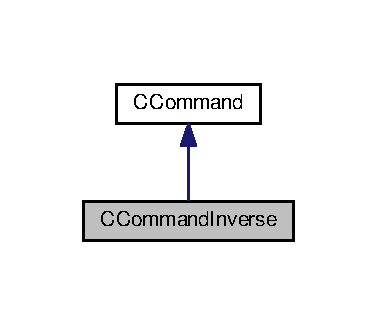
\includegraphics[width=181pt]{classCCommandInverse__inherit__graph}
\end{center}
\end{figure}


Collaboration diagram for C\+Command\+Inverse\+:\nopagebreak
\begin{figure}[H]
\begin{center}
\leavevmode
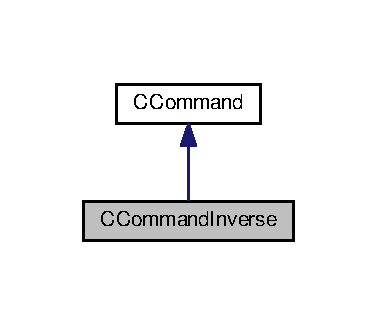
\includegraphics[width=181pt]{classCCommandInverse__coll__graph}
\end{center}
\end{figure}
\subsection*{Public Member Functions}
\begin{DoxyCompactItemize}
\item 
\hyperlink{classCCommandInverse_a9573921cedbcfd0a0e5e16157e120855}{C\+Command\+Inverse} ()
\item 
\hyperlink{classCCommandInverse_adb4a4a3be76c91fbfb8cbefb920fd4d1}{$\sim$\+C\+Command\+Inverse} () override=default
\item 
\hyperlink{classCCommandInverse_a7b55a6f59f8dd6ae62e44297cf6c6740}{C\+Command\+Inverse} (string var\+Name)
\item 
bool \hyperlink{classCCommandInverse_aa579b94f10fa18b4759fd2986629f7db}{Execute} (\hyperlink{classCMemory}{C\+Memory} \&memory) override
\end{DoxyCompactItemize}
\subsection*{Private Attributes}
\begin{DoxyCompactItemize}
\item 
string \hyperlink{classCCommandInverse_a0808798ecacedd86196ba9812ce64d4f}{m\+\_\+\+Var\+Name}
\end{DoxyCompactItemize}
\subsection*{Additional Inherited Members}


\subsection{Constructor \& Destructor Documentation}
\index{C\+Command\+Inverse@{C\+Command\+Inverse}!C\+Command\+Inverse@{C\+Command\+Inverse}}
\index{C\+Command\+Inverse@{C\+Command\+Inverse}!C\+Command\+Inverse@{C\+Command\+Inverse}}
\subsubsection[{\texorpdfstring{C\+Command\+Inverse()}{CCommandInverse()}}]{\setlength{\rightskip}{0pt plus 5cm}C\+Command\+Inverse\+::\+C\+Command\+Inverse (
\begin{DoxyParamCaption}
{}
\end{DoxyParamCaption}
)\hspace{0.3cm}{\ttfamily [inline]}}\hypertarget{classCCommandInverse_a9573921cedbcfd0a0e5e16157e120855}{}\label{classCCommandInverse_a9573921cedbcfd0a0e5e16157e120855}
\index{C\+Command\+Inverse@{C\+Command\+Inverse}!````~C\+Command\+Inverse@{$\sim$\+C\+Command\+Inverse}}
\index{````~C\+Command\+Inverse@{$\sim$\+C\+Command\+Inverse}!C\+Command\+Inverse@{C\+Command\+Inverse}}
\subsubsection[{\texorpdfstring{$\sim$\+C\+Command\+Inverse() override=default}{~CCommandInverse() override=default}}]{\setlength{\rightskip}{0pt plus 5cm}C\+Command\+Inverse\+::$\sim$\+C\+Command\+Inverse (
\begin{DoxyParamCaption}
{}
\end{DoxyParamCaption}
)\hspace{0.3cm}{\ttfamily [override]}, {\ttfamily [default]}}\hypertarget{classCCommandInverse_adb4a4a3be76c91fbfb8cbefb920fd4d1}{}\label{classCCommandInverse_adb4a4a3be76c91fbfb8cbefb920fd4d1}
\index{C\+Command\+Inverse@{C\+Command\+Inverse}!C\+Command\+Inverse@{C\+Command\+Inverse}}
\index{C\+Command\+Inverse@{C\+Command\+Inverse}!C\+Command\+Inverse@{C\+Command\+Inverse}}
\subsubsection[{\texorpdfstring{C\+Command\+Inverse(string var\+Name)}{CCommandInverse(string varName)}}]{\setlength{\rightskip}{0pt plus 5cm}C\+Command\+Inverse\+::\+C\+Command\+Inverse (
\begin{DoxyParamCaption}
\item[{string}]{var\+Name}
\end{DoxyParamCaption}
)\hspace{0.3cm}{\ttfamily [inline]}}\hypertarget{classCCommandInverse_a7b55a6f59f8dd6ae62e44297cf6c6740}{}\label{classCCommandInverse_a7b55a6f59f8dd6ae62e44297cf6c6740}


\subsection{Member Function Documentation}
\index{C\+Command\+Inverse@{C\+Command\+Inverse}!Execute@{Execute}}
\index{Execute@{Execute}!C\+Command\+Inverse@{C\+Command\+Inverse}}
\subsubsection[{\texorpdfstring{Execute(\+C\+Memory \&memory) override}{Execute(CMemory &memory) override}}]{\setlength{\rightskip}{0pt plus 5cm}bool C\+Command\+Inverse\+::\+Execute (
\begin{DoxyParamCaption}
\item[{{\bf C\+Memory} \&}]{memory}
\end{DoxyParamCaption}
)\hspace{0.3cm}{\ttfamily [override]}, {\ttfamily [virtual]}}\hypertarget{classCCommandInverse_aa579b94f10fa18b4759fd2986629f7db}{}\label{classCCommandInverse_aa579b94f10fa18b4759fd2986629f7db}
Execute command. 
\begin{DoxyParams}{Parameters}
{\em memory} & \\
\hline
\end{DoxyParams}
\begin{DoxyReturn}{Returns}
true if execution successful, false otherwise (command cannot be performed) 
\end{DoxyReturn}


Implements \hyperlink{classCCommand_ad9361ea814093c4ebecf22bb0a3f8b79}{C\+Command}.



\subsection{Member Data Documentation}
\index{C\+Command\+Inverse@{C\+Command\+Inverse}!m\+\_\+\+Var\+Name@{m\+\_\+\+Var\+Name}}
\index{m\+\_\+\+Var\+Name@{m\+\_\+\+Var\+Name}!C\+Command\+Inverse@{C\+Command\+Inverse}}
\subsubsection[{\texorpdfstring{m\+\_\+\+Var\+Name}{m_VarName}}]{\setlength{\rightskip}{0pt plus 5cm}string C\+Command\+Inverse\+::m\+\_\+\+Var\+Name\hspace{0.3cm}{\ttfamily [private]}}\hypertarget{classCCommandInverse_a0808798ecacedd86196ba9812ce64d4f}{}\label{classCCommandInverse_a0808798ecacedd86196ba9812ce64d4f}


The documentation for this class was generated from the following files\+:\begin{DoxyCompactItemize}
\item 
src/\hyperlink{CCommandInverse_8h}{C\+Command\+Inverse.\+h}\item 
src/\hyperlink{CCommandInverse_8cpp}{C\+Command\+Inverse.\+cpp}\end{DoxyCompactItemize}

\hypertarget{classCCommandLoad}{}\section{C\+Command\+Load Class Reference}
\label{classCCommandLoad}\index{C\+Command\+Load@{C\+Command\+Load}}


{\ttfamily \#include $<$C\+Command\+Load.\+h$>$}



Inheritance diagram for C\+Command\+Load\+:\nopagebreak
\begin{figure}[H]
\begin{center}
\leavevmode
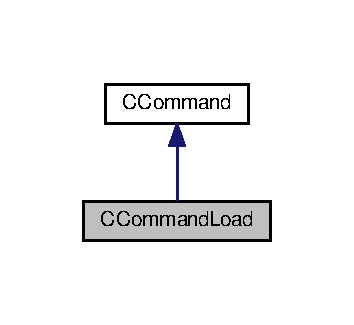
\includegraphics[width=170pt]{classCCommandLoad__inherit__graph}
\end{center}
\end{figure}


Collaboration diagram for C\+Command\+Load\+:\nopagebreak
\begin{figure}[H]
\begin{center}
\leavevmode
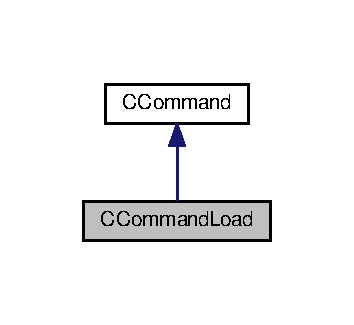
\includegraphics[width=170pt]{classCCommandLoad__coll__graph}
\end{center}
\end{figure}
\subsection*{Public Member Functions}
\begin{DoxyCompactItemize}
\item 
\hyperlink{classCCommandLoad_a88702ae3cce0d9197c6a58d2726952f9}{C\+Command\+Load} ()
\item 
\hyperlink{classCCommandLoad_a6430e6c5bb123b4a22a153b705655b6c}{$\sim$\+C\+Command\+Load} () override=default
\item 
\hyperlink{classCCommandLoad_aa53bda871a5d4d8af9fbdbc0e4d0ffe3}{C\+Command\+Load} (string var\+Name, vector$<$ vector$<$ double $>$$>$ matrix\+Nums)
\item 
bool \hyperlink{classCCommandLoad_a5940ee064de6b5497e9b868b1add9880}{Execute} (\hyperlink{classCMemory}{C\+Memory} \&memory) override
\end{DoxyCompactItemize}
\subsection*{Private Attributes}
\begin{DoxyCompactItemize}
\item 
string \hyperlink{classCCommandLoad_a0158c8f9882c1a82bba09ccefa67ed12}{m\+\_\+\+Variable\+Name}
\end{DoxyCompactItemize}
\subsection*{Additional Inherited Members}


\subsection{Constructor \& Destructor Documentation}
\index{C\+Command\+Load@{C\+Command\+Load}!C\+Command\+Load@{C\+Command\+Load}}
\index{C\+Command\+Load@{C\+Command\+Load}!C\+Command\+Load@{C\+Command\+Load}}
\subsubsection[{\texorpdfstring{C\+Command\+Load()}{CCommandLoad()}}]{\setlength{\rightskip}{0pt plus 5cm}C\+Command\+Load\+::\+C\+Command\+Load (
\begin{DoxyParamCaption}
{}
\end{DoxyParamCaption}
)\hspace{0.3cm}{\ttfamily [inline]}}\hypertarget{classCCommandLoad_a88702ae3cce0d9197c6a58d2726952f9}{}\label{classCCommandLoad_a88702ae3cce0d9197c6a58d2726952f9}
\index{C\+Command\+Load@{C\+Command\+Load}!````~C\+Command\+Load@{$\sim$\+C\+Command\+Load}}
\index{````~C\+Command\+Load@{$\sim$\+C\+Command\+Load}!C\+Command\+Load@{C\+Command\+Load}}
\subsubsection[{\texorpdfstring{$\sim$\+C\+Command\+Load() override=default}{~CCommandLoad() override=default}}]{\setlength{\rightskip}{0pt plus 5cm}C\+Command\+Load\+::$\sim$\+C\+Command\+Load (
\begin{DoxyParamCaption}
{}
\end{DoxyParamCaption}
)\hspace{0.3cm}{\ttfamily [override]}, {\ttfamily [default]}}\hypertarget{classCCommandLoad_a6430e6c5bb123b4a22a153b705655b6c}{}\label{classCCommandLoad_a6430e6c5bb123b4a22a153b705655b6c}
\index{C\+Command\+Load@{C\+Command\+Load}!C\+Command\+Load@{C\+Command\+Load}}
\index{C\+Command\+Load@{C\+Command\+Load}!C\+Command\+Load@{C\+Command\+Load}}
\subsubsection[{\texorpdfstring{C\+Command\+Load(string var\+Name, vector$<$ vector$<$ double $>$$>$ matrix\+Nums)}{CCommandLoad(string varName, vector< vector< double >> matrixNums)}}]{\setlength{\rightskip}{0pt plus 5cm}C\+Command\+Load\+::\+C\+Command\+Load (
\begin{DoxyParamCaption}
\item[{string}]{var\+Name, }
\item[{vector$<$ vector$<$ double $>$$>$}]{matrix\+Nums}
\end{DoxyParamCaption}
)\hspace{0.3cm}{\ttfamily [inline]}}\hypertarget{classCCommandLoad_aa53bda871a5d4d8af9fbdbc0e4d0ffe3}{}\label{classCCommandLoad_aa53bda871a5d4d8af9fbdbc0e4d0ffe3}


\subsection{Member Function Documentation}
\index{C\+Command\+Load@{C\+Command\+Load}!Execute@{Execute}}
\index{Execute@{Execute}!C\+Command\+Load@{C\+Command\+Load}}
\subsubsection[{\texorpdfstring{Execute(\+C\+Memory \&memory) override}{Execute(CMemory &memory) override}}]{\setlength{\rightskip}{0pt plus 5cm}bool C\+Command\+Load\+::\+Execute (
\begin{DoxyParamCaption}
\item[{{\bf C\+Memory} \&}]{memory}
\end{DoxyParamCaption}
)\hspace{0.3cm}{\ttfamily [inline]}, {\ttfamily [override]}, {\ttfamily [virtual]}}\hypertarget{classCCommandLoad_a5940ee064de6b5497e9b868b1add9880}{}\label{classCCommandLoad_a5940ee064de6b5497e9b868b1add9880}


Implements \hyperlink{classCCommand_ad9361ea814093c4ebecf22bb0a3f8b79}{C\+Command}.



\subsection{Member Data Documentation}
\index{C\+Command\+Load@{C\+Command\+Load}!m\+\_\+\+Variable\+Name@{m\+\_\+\+Variable\+Name}}
\index{m\+\_\+\+Variable\+Name@{m\+\_\+\+Variable\+Name}!C\+Command\+Load@{C\+Command\+Load}}
\subsubsection[{\texorpdfstring{m\+\_\+\+Variable\+Name}{m_VariableName}}]{\setlength{\rightskip}{0pt plus 5cm}string C\+Command\+Load\+::m\+\_\+\+Variable\+Name\hspace{0.3cm}{\ttfamily [private]}}\hypertarget{classCCommandLoad_a0158c8f9882c1a82bba09ccefa67ed12}{}\label{classCCommandLoad_a0158c8f9882c1a82bba09ccefa67ed12}


The documentation for this class was generated from the following file\+:\begin{DoxyCompactItemize}
\item 
src/\hyperlink{CCommandLoad_8h}{C\+Command\+Load.\+h}\end{DoxyCompactItemize}

\hypertarget{classCCommandMergeNextTo}{}\section{C\+Command\+Merge\+Next\+To Class Reference}
\label{classCCommandMergeNextTo}\index{C\+Command\+Merge\+Next\+To@{C\+Command\+Merge\+Next\+To}}


{\ttfamily \#include $<$C\+Command\+Merge\+Next\+To.\+h$>$}



Inheritance diagram for C\+Command\+Merge\+Next\+To\+:\nopagebreak
\begin{figure}[H]
\begin{center}
\leavevmode
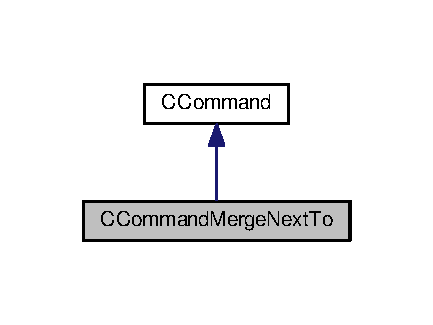
\includegraphics[width=208pt]{classCCommandMergeNextTo__inherit__graph}
\end{center}
\end{figure}


Collaboration diagram for C\+Command\+Merge\+Next\+To\+:\nopagebreak
\begin{figure}[H]
\begin{center}
\leavevmode
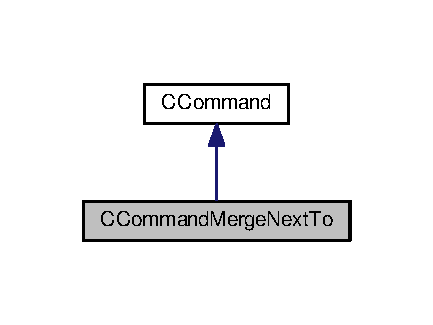
\includegraphics[width=208pt]{classCCommandMergeNextTo__coll__graph}
\end{center}
\end{figure}
\subsection*{Public Member Functions}
\begin{DoxyCompactItemize}
\item 
\hyperlink{classCCommandMergeNextTo_a2397e4c98e3fa492a810a52e58600a2d}{C\+Command\+Merge\+Next\+To} ()
\item 
\hyperlink{classCCommandMergeNextTo_a30710620440575d837b11d52eec0bde0}{$\sim$\+C\+Command\+Merge\+Next\+To} () override=default
\item 
\hyperlink{classCCommandMergeNextTo_af7978b80e72315e0a82f66da589fac2f}{C\+Command\+Merge\+Next\+To} (string operand1, string operand2)
\item 
bool \hyperlink{classCCommandMergeNextTo_acca1ef026b0bad3d44f1e4ba09276361}{Execute} (\hyperlink{classCMemory}{C\+Memory} \&memory) override
\end{DoxyCompactItemize}
\subsection*{Private Attributes}
\begin{DoxyCompactItemize}
\item 
string \hyperlink{classCCommandMergeNextTo_ae967c718f405476f0a833994061af64f}{m\+\_\+\+Operand1}
\item 
string \hyperlink{classCCommandMergeNextTo_a201710d63a46fee8603ee4b625e8e189}{m\+\_\+\+Operand2}
\end{DoxyCompactItemize}
\subsection*{Additional Inherited Members}


\subsection{Constructor \& Destructor Documentation}
\index{C\+Command\+Merge\+Next\+To@{C\+Command\+Merge\+Next\+To}!C\+Command\+Merge\+Next\+To@{C\+Command\+Merge\+Next\+To}}
\index{C\+Command\+Merge\+Next\+To@{C\+Command\+Merge\+Next\+To}!C\+Command\+Merge\+Next\+To@{C\+Command\+Merge\+Next\+To}}
\subsubsection[{\texorpdfstring{C\+Command\+Merge\+Next\+To()}{CCommandMergeNextTo()}}]{\setlength{\rightskip}{0pt plus 5cm}C\+Command\+Merge\+Next\+To\+::\+C\+Command\+Merge\+Next\+To (
\begin{DoxyParamCaption}
{}
\end{DoxyParamCaption}
)\hspace{0.3cm}{\ttfamily [inline]}}\hypertarget{classCCommandMergeNextTo_a2397e4c98e3fa492a810a52e58600a2d}{}\label{classCCommandMergeNextTo_a2397e4c98e3fa492a810a52e58600a2d}
\index{C\+Command\+Merge\+Next\+To@{C\+Command\+Merge\+Next\+To}!````~C\+Command\+Merge\+Next\+To@{$\sim$\+C\+Command\+Merge\+Next\+To}}
\index{````~C\+Command\+Merge\+Next\+To@{$\sim$\+C\+Command\+Merge\+Next\+To}!C\+Command\+Merge\+Next\+To@{C\+Command\+Merge\+Next\+To}}
\subsubsection[{\texorpdfstring{$\sim$\+C\+Command\+Merge\+Next\+To() override=default}{~CCommandMergeNextTo() override=default}}]{\setlength{\rightskip}{0pt plus 5cm}C\+Command\+Merge\+Next\+To\+::$\sim$\+C\+Command\+Merge\+Next\+To (
\begin{DoxyParamCaption}
{}
\end{DoxyParamCaption}
)\hspace{0.3cm}{\ttfamily [override]}, {\ttfamily [default]}}\hypertarget{classCCommandMergeNextTo_a30710620440575d837b11d52eec0bde0}{}\label{classCCommandMergeNextTo_a30710620440575d837b11d52eec0bde0}
\index{C\+Command\+Merge\+Next\+To@{C\+Command\+Merge\+Next\+To}!C\+Command\+Merge\+Next\+To@{C\+Command\+Merge\+Next\+To}}
\index{C\+Command\+Merge\+Next\+To@{C\+Command\+Merge\+Next\+To}!C\+Command\+Merge\+Next\+To@{C\+Command\+Merge\+Next\+To}}
\subsubsection[{\texorpdfstring{C\+Command\+Merge\+Next\+To(string operand1, string operand2)}{CCommandMergeNextTo(string operand1, string operand2)}}]{\setlength{\rightskip}{0pt plus 5cm}C\+Command\+Merge\+Next\+To\+::\+C\+Command\+Merge\+Next\+To (
\begin{DoxyParamCaption}
\item[{string}]{operand1, }
\item[{string}]{operand2}
\end{DoxyParamCaption}
)\hspace{0.3cm}{\ttfamily [inline]}}\hypertarget{classCCommandMergeNextTo_af7978b80e72315e0a82f66da589fac2f}{}\label{classCCommandMergeNextTo_af7978b80e72315e0a82f66da589fac2f}


\subsection{Member Function Documentation}
\index{C\+Command\+Merge\+Next\+To@{C\+Command\+Merge\+Next\+To}!Execute@{Execute}}
\index{Execute@{Execute}!C\+Command\+Merge\+Next\+To@{C\+Command\+Merge\+Next\+To}}
\subsubsection[{\texorpdfstring{Execute(\+C\+Memory \&memory) override}{Execute(CMemory &memory) override}}]{\setlength{\rightskip}{0pt plus 5cm}bool C\+Command\+Merge\+Next\+To\+::\+Execute (
\begin{DoxyParamCaption}
\item[{{\bf C\+Memory} \&}]{memory}
\end{DoxyParamCaption}
)\hspace{0.3cm}{\ttfamily [inline]}, {\ttfamily [override]}, {\ttfamily [virtual]}}\hypertarget{classCCommandMergeNextTo_acca1ef026b0bad3d44f1e4ba09276361}{}\label{classCCommandMergeNextTo_acca1ef026b0bad3d44f1e4ba09276361}


Implements \hyperlink{classCCommand_ad9361ea814093c4ebecf22bb0a3f8b79}{C\+Command}.



\subsection{Member Data Documentation}
\index{C\+Command\+Merge\+Next\+To@{C\+Command\+Merge\+Next\+To}!m\+\_\+\+Operand1@{m\+\_\+\+Operand1}}
\index{m\+\_\+\+Operand1@{m\+\_\+\+Operand1}!C\+Command\+Merge\+Next\+To@{C\+Command\+Merge\+Next\+To}}
\subsubsection[{\texorpdfstring{m\+\_\+\+Operand1}{m_Operand1}}]{\setlength{\rightskip}{0pt plus 5cm}string C\+Command\+Merge\+Next\+To\+::m\+\_\+\+Operand1\hspace{0.3cm}{\ttfamily [private]}}\hypertarget{classCCommandMergeNextTo_ae967c718f405476f0a833994061af64f}{}\label{classCCommandMergeNextTo_ae967c718f405476f0a833994061af64f}
\index{C\+Command\+Merge\+Next\+To@{C\+Command\+Merge\+Next\+To}!m\+\_\+\+Operand2@{m\+\_\+\+Operand2}}
\index{m\+\_\+\+Operand2@{m\+\_\+\+Operand2}!C\+Command\+Merge\+Next\+To@{C\+Command\+Merge\+Next\+To}}
\subsubsection[{\texorpdfstring{m\+\_\+\+Operand2}{m_Operand2}}]{\setlength{\rightskip}{0pt plus 5cm}string C\+Command\+Merge\+Next\+To\+::m\+\_\+\+Operand2\hspace{0.3cm}{\ttfamily [private]}}\hypertarget{classCCommandMergeNextTo_a201710d63a46fee8603ee4b625e8e189}{}\label{classCCommandMergeNextTo_a201710d63a46fee8603ee4b625e8e189}


The documentation for this class was generated from the following file\+:\begin{DoxyCompactItemize}
\item 
src/\hyperlink{CCommandMergeNextTo_8h}{C\+Command\+Merge\+Next\+To.\+h}\end{DoxyCompactItemize}

\hypertarget{classCCommandMergeUnder}{}\section{C\+Command\+Merge\+Under Class Reference}
\label{classCCommandMergeUnder}\index{C\+Command\+Merge\+Under@{C\+Command\+Merge\+Under}}


{\ttfamily \#include $<$C\+Command\+Merge\+Under.\+h$>$}



Inheritance diagram for C\+Command\+Merge\+Under\+:\nopagebreak
\begin{figure}[H]
\begin{center}
\leavevmode
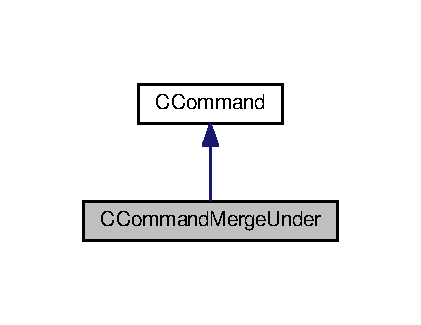
\includegraphics[width=202pt]{classCCommandMergeUnder__inherit__graph}
\end{center}
\end{figure}


Collaboration diagram for C\+Command\+Merge\+Under\+:\nopagebreak
\begin{figure}[H]
\begin{center}
\leavevmode
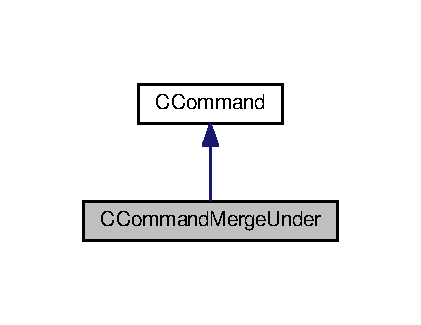
\includegraphics[width=202pt]{classCCommandMergeUnder__coll__graph}
\end{center}
\end{figure}
\subsection*{Public Member Functions}
\begin{DoxyCompactItemize}
\item 
\hyperlink{classCCommandMergeUnder_a449c38d9105e8f9c9d2d7251ca215c0b}{C\+Command\+Merge\+Under} ()
\item 
\hyperlink{classCCommandMergeUnder_a6985544ad20321eb080a88799b7d6235}{$\sim$\+C\+Command\+Merge\+Under} () override=default
\item 
\hyperlink{classCCommandMergeUnder_a4db178e9f87c809bae06550786bfe2eb}{C\+Command\+Merge\+Under} (string operand1, string operand2)
\item 
bool \hyperlink{classCCommandMergeUnder_abf1fb6fe63188e0ba0dc82dfa7bac083}{Execute} (\hyperlink{classCMemory}{C\+Memory} \&memory) override
\end{DoxyCompactItemize}
\subsection*{Private Attributes}
\begin{DoxyCompactItemize}
\item 
string \hyperlink{classCCommandMergeUnder_abeada56729aa197e14779621c7eb03c0}{m\+\_\+\+Operand1}
\item 
string \hyperlink{classCCommandMergeUnder_adfb43ee9af1ba4ba89e49b63a08b0cba}{m\+\_\+\+Operand2}
\end{DoxyCompactItemize}
\subsection*{Additional Inherited Members}


\subsection{Constructor \& Destructor Documentation}
\index{C\+Command\+Merge\+Under@{C\+Command\+Merge\+Under}!C\+Command\+Merge\+Under@{C\+Command\+Merge\+Under}}
\index{C\+Command\+Merge\+Under@{C\+Command\+Merge\+Under}!C\+Command\+Merge\+Under@{C\+Command\+Merge\+Under}}
\subsubsection[{\texorpdfstring{C\+Command\+Merge\+Under()}{CCommandMergeUnder()}}]{\setlength{\rightskip}{0pt plus 5cm}C\+Command\+Merge\+Under\+::\+C\+Command\+Merge\+Under (
\begin{DoxyParamCaption}
{}
\end{DoxyParamCaption}
)\hspace{0.3cm}{\ttfamily [inline]}}\hypertarget{classCCommandMergeUnder_a449c38d9105e8f9c9d2d7251ca215c0b}{}\label{classCCommandMergeUnder_a449c38d9105e8f9c9d2d7251ca215c0b}
\index{C\+Command\+Merge\+Under@{C\+Command\+Merge\+Under}!````~C\+Command\+Merge\+Under@{$\sim$\+C\+Command\+Merge\+Under}}
\index{````~C\+Command\+Merge\+Under@{$\sim$\+C\+Command\+Merge\+Under}!C\+Command\+Merge\+Under@{C\+Command\+Merge\+Under}}
\subsubsection[{\texorpdfstring{$\sim$\+C\+Command\+Merge\+Under() override=default}{~CCommandMergeUnder() override=default}}]{\setlength{\rightskip}{0pt plus 5cm}C\+Command\+Merge\+Under\+::$\sim$\+C\+Command\+Merge\+Under (
\begin{DoxyParamCaption}
{}
\end{DoxyParamCaption}
)\hspace{0.3cm}{\ttfamily [override]}, {\ttfamily [default]}}\hypertarget{classCCommandMergeUnder_a6985544ad20321eb080a88799b7d6235}{}\label{classCCommandMergeUnder_a6985544ad20321eb080a88799b7d6235}
\index{C\+Command\+Merge\+Under@{C\+Command\+Merge\+Under}!C\+Command\+Merge\+Under@{C\+Command\+Merge\+Under}}
\index{C\+Command\+Merge\+Under@{C\+Command\+Merge\+Under}!C\+Command\+Merge\+Under@{C\+Command\+Merge\+Under}}
\subsubsection[{\texorpdfstring{C\+Command\+Merge\+Under(string operand1, string operand2)}{CCommandMergeUnder(string operand1, string operand2)}}]{\setlength{\rightskip}{0pt plus 5cm}C\+Command\+Merge\+Under\+::\+C\+Command\+Merge\+Under (
\begin{DoxyParamCaption}
\item[{string}]{operand1, }
\item[{string}]{operand2}
\end{DoxyParamCaption}
)\hspace{0.3cm}{\ttfamily [inline]}}\hypertarget{classCCommandMergeUnder_a4db178e9f87c809bae06550786bfe2eb}{}\label{classCCommandMergeUnder_a4db178e9f87c809bae06550786bfe2eb}


\subsection{Member Function Documentation}
\index{C\+Command\+Merge\+Under@{C\+Command\+Merge\+Under}!Execute@{Execute}}
\index{Execute@{Execute}!C\+Command\+Merge\+Under@{C\+Command\+Merge\+Under}}
\subsubsection[{\texorpdfstring{Execute(\+C\+Memory \&memory) override}{Execute(CMemory &memory) override}}]{\setlength{\rightskip}{0pt plus 5cm}bool C\+Command\+Merge\+Under\+::\+Execute (
\begin{DoxyParamCaption}
\item[{{\bf C\+Memory} \&}]{memory}
\end{DoxyParamCaption}
)\hspace{0.3cm}{\ttfamily [override]}, {\ttfamily [virtual]}}\hypertarget{classCCommandMergeUnder_abf1fb6fe63188e0ba0dc82dfa7bac083}{}\label{classCCommandMergeUnder_abf1fb6fe63188e0ba0dc82dfa7bac083}
Execute command. 
\begin{DoxyParams}{Parameters}
{\em memory} & \\
\hline
\end{DoxyParams}
\begin{DoxyReturn}{Returns}
true if execution successful, false otherwise (command cannot be performed) 
\end{DoxyReturn}


Implements \hyperlink{classCCommand_ad9361ea814093c4ebecf22bb0a3f8b79}{C\+Command}.



\subsection{Member Data Documentation}
\index{C\+Command\+Merge\+Under@{C\+Command\+Merge\+Under}!m\+\_\+\+Operand1@{m\+\_\+\+Operand1}}
\index{m\+\_\+\+Operand1@{m\+\_\+\+Operand1}!C\+Command\+Merge\+Under@{C\+Command\+Merge\+Under}}
\subsubsection[{\texorpdfstring{m\+\_\+\+Operand1}{m_Operand1}}]{\setlength{\rightskip}{0pt plus 5cm}string C\+Command\+Merge\+Under\+::m\+\_\+\+Operand1\hspace{0.3cm}{\ttfamily [private]}}\hypertarget{classCCommandMergeUnder_abeada56729aa197e14779621c7eb03c0}{}\label{classCCommandMergeUnder_abeada56729aa197e14779621c7eb03c0}
\index{C\+Command\+Merge\+Under@{C\+Command\+Merge\+Under}!m\+\_\+\+Operand2@{m\+\_\+\+Operand2}}
\index{m\+\_\+\+Operand2@{m\+\_\+\+Operand2}!C\+Command\+Merge\+Under@{C\+Command\+Merge\+Under}}
\subsubsection[{\texorpdfstring{m\+\_\+\+Operand2}{m_Operand2}}]{\setlength{\rightskip}{0pt plus 5cm}string C\+Command\+Merge\+Under\+::m\+\_\+\+Operand2\hspace{0.3cm}{\ttfamily [private]}}\hypertarget{classCCommandMergeUnder_adfb43ee9af1ba4ba89e49b63a08b0cba}{}\label{classCCommandMergeUnder_adfb43ee9af1ba4ba89e49b63a08b0cba}


The documentation for this class was generated from the following files\+:\begin{DoxyCompactItemize}
\item 
src/\hyperlink{CCommandMergeUnder_8h}{C\+Command\+Merge\+Under.\+h}\item 
src/\hyperlink{CCommandMergeUnder_8cpp}{C\+Command\+Merge\+Under.\+cpp}\end{DoxyCompactItemize}

\hypertarget{classCCommandMultiply}{}\section{C\+Command\+Multiply Class Reference}
\label{classCCommandMultiply}\index{C\+Command\+Multiply@{C\+Command\+Multiply}}


{\ttfamily \#include $<$C\+Command\+Multiply.\+h$>$}



Inheritance diagram for C\+Command\+Multiply\+:\nopagebreak
\begin{figure}[H]
\begin{center}
\leavevmode
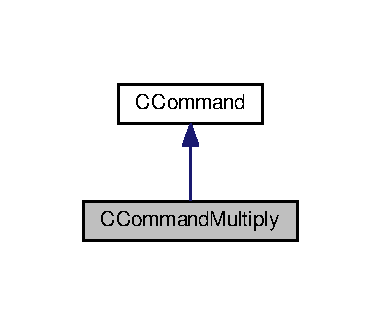
\includegraphics[width=183pt]{classCCommandMultiply__inherit__graph}
\end{center}
\end{figure}


Collaboration diagram for C\+Command\+Multiply\+:\nopagebreak
\begin{figure}[H]
\begin{center}
\leavevmode
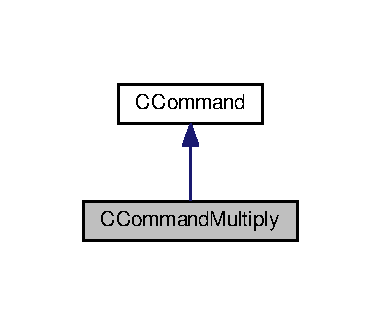
\includegraphics[width=183pt]{classCCommandMultiply__coll__graph}
\end{center}
\end{figure}
\subsection*{Public Member Functions}
\begin{DoxyCompactItemize}
\item 
\hyperlink{classCCommandMultiply_a197041ecfb102aaf78c87d5e283cc9c1}{C\+Command\+Multiply} ()
\item 
\hyperlink{classCCommandMultiply_a791709da46cb4b6578880d65ecfa304a}{$\sim$\+C\+Command\+Multiply} () override=default
\item 
\hyperlink{classCCommandMultiply_abdd4d23d9a7c8aeecfc2a32e365759a9}{C\+Command\+Multiply} (string operand1, string operand2)
\item 
bool \hyperlink{classCCommandMultiply_a06d75c2d7c89607406de6c05e586907f}{Execute} (\hyperlink{classCMemory}{C\+Memory} \&memory) override
\end{DoxyCompactItemize}
\subsection*{Private Attributes}
\begin{DoxyCompactItemize}
\item 
string \hyperlink{classCCommandMultiply_a41c3f181f0ee844a3afaba12a96c4502}{m\+\_\+\+Operand1}
\item 
string \hyperlink{classCCommandMultiply_a213170d1398739645e55e5e841fff405}{m\+\_\+\+Operand2}
\end{DoxyCompactItemize}
\subsection*{Additional Inherited Members}


\subsection{Constructor \& Destructor Documentation}
\index{C\+Command\+Multiply@{C\+Command\+Multiply}!C\+Command\+Multiply@{C\+Command\+Multiply}}
\index{C\+Command\+Multiply@{C\+Command\+Multiply}!C\+Command\+Multiply@{C\+Command\+Multiply}}
\subsubsection[{\texorpdfstring{C\+Command\+Multiply()}{CCommandMultiply()}}]{\setlength{\rightskip}{0pt plus 5cm}C\+Command\+Multiply\+::\+C\+Command\+Multiply (
\begin{DoxyParamCaption}
{}
\end{DoxyParamCaption}
)\hspace{0.3cm}{\ttfamily [inline]}}\hypertarget{classCCommandMultiply_a197041ecfb102aaf78c87d5e283cc9c1}{}\label{classCCommandMultiply_a197041ecfb102aaf78c87d5e283cc9c1}
\index{C\+Command\+Multiply@{C\+Command\+Multiply}!````~C\+Command\+Multiply@{$\sim$\+C\+Command\+Multiply}}
\index{````~C\+Command\+Multiply@{$\sim$\+C\+Command\+Multiply}!C\+Command\+Multiply@{C\+Command\+Multiply}}
\subsubsection[{\texorpdfstring{$\sim$\+C\+Command\+Multiply() override=default}{~CCommandMultiply() override=default}}]{\setlength{\rightskip}{0pt plus 5cm}C\+Command\+Multiply\+::$\sim$\+C\+Command\+Multiply (
\begin{DoxyParamCaption}
{}
\end{DoxyParamCaption}
)\hspace{0.3cm}{\ttfamily [override]}, {\ttfamily [default]}}\hypertarget{classCCommandMultiply_a791709da46cb4b6578880d65ecfa304a}{}\label{classCCommandMultiply_a791709da46cb4b6578880d65ecfa304a}
\index{C\+Command\+Multiply@{C\+Command\+Multiply}!C\+Command\+Multiply@{C\+Command\+Multiply}}
\index{C\+Command\+Multiply@{C\+Command\+Multiply}!C\+Command\+Multiply@{C\+Command\+Multiply}}
\subsubsection[{\texorpdfstring{C\+Command\+Multiply(string operand1, string operand2)}{CCommandMultiply(string operand1, string operand2)}}]{\setlength{\rightskip}{0pt plus 5cm}C\+Command\+Multiply\+::\+C\+Command\+Multiply (
\begin{DoxyParamCaption}
\item[{string}]{operand1, }
\item[{string}]{operand2}
\end{DoxyParamCaption}
)\hspace{0.3cm}{\ttfamily [inline]}}\hypertarget{classCCommandMultiply_abdd4d23d9a7c8aeecfc2a32e365759a9}{}\label{classCCommandMultiply_abdd4d23d9a7c8aeecfc2a32e365759a9}


\subsection{Member Function Documentation}
\index{C\+Command\+Multiply@{C\+Command\+Multiply}!Execute@{Execute}}
\index{Execute@{Execute}!C\+Command\+Multiply@{C\+Command\+Multiply}}
\subsubsection[{\texorpdfstring{Execute(\+C\+Memory \&memory) override}{Execute(CMemory &memory) override}}]{\setlength{\rightskip}{0pt plus 5cm}bool C\+Command\+Multiply\+::\+Execute (
\begin{DoxyParamCaption}
\item[{{\bf C\+Memory} \&}]{memory}
\end{DoxyParamCaption}
)\hspace{0.3cm}{\ttfamily [inline]}, {\ttfamily [override]}, {\ttfamily [virtual]}}\hypertarget{classCCommandMultiply_a06d75c2d7c89607406de6c05e586907f}{}\label{classCCommandMultiply_a06d75c2d7c89607406de6c05e586907f}


Implements \hyperlink{classCCommand_ad9361ea814093c4ebecf22bb0a3f8b79}{C\+Command}.



\subsection{Member Data Documentation}
\index{C\+Command\+Multiply@{C\+Command\+Multiply}!m\+\_\+\+Operand1@{m\+\_\+\+Operand1}}
\index{m\+\_\+\+Operand1@{m\+\_\+\+Operand1}!C\+Command\+Multiply@{C\+Command\+Multiply}}
\subsubsection[{\texorpdfstring{m\+\_\+\+Operand1}{m_Operand1}}]{\setlength{\rightskip}{0pt plus 5cm}string C\+Command\+Multiply\+::m\+\_\+\+Operand1\hspace{0.3cm}{\ttfamily [private]}}\hypertarget{classCCommandMultiply_a41c3f181f0ee844a3afaba12a96c4502}{}\label{classCCommandMultiply_a41c3f181f0ee844a3afaba12a96c4502}
\index{C\+Command\+Multiply@{C\+Command\+Multiply}!m\+\_\+\+Operand2@{m\+\_\+\+Operand2}}
\index{m\+\_\+\+Operand2@{m\+\_\+\+Operand2}!C\+Command\+Multiply@{C\+Command\+Multiply}}
\subsubsection[{\texorpdfstring{m\+\_\+\+Operand2}{m_Operand2}}]{\setlength{\rightskip}{0pt plus 5cm}string C\+Command\+Multiply\+::m\+\_\+\+Operand2\hspace{0.3cm}{\ttfamily [private]}}\hypertarget{classCCommandMultiply_a213170d1398739645e55e5e841fff405}{}\label{classCCommandMultiply_a213170d1398739645e55e5e841fff405}


The documentation for this class was generated from the following file\+:\begin{DoxyCompactItemize}
\item 
src/\hyperlink{CCommandMultiply_8h}{C\+Command\+Multiply.\+h}\end{DoxyCompactItemize}

\hypertarget{classCCommandOrder}{}\section{C\+Command\+Order Class Reference}
\label{classCCommandOrder}\index{C\+Command\+Order@{C\+Command\+Order}}


{\ttfamily \#include $<$C\+Command\+Order.\+h$>$}



Inheritance diagram for C\+Command\+Order\+:\nopagebreak
\begin{figure}[H]
\begin{center}
\leavevmode
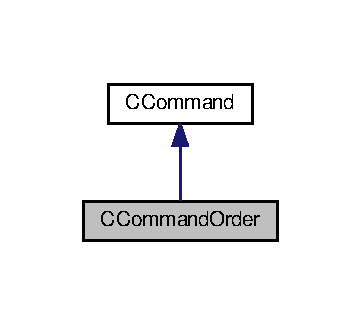
\includegraphics[width=173pt]{classCCommandOrder__inherit__graph}
\end{center}
\end{figure}


Collaboration diagram for C\+Command\+Order\+:\nopagebreak
\begin{figure}[H]
\begin{center}
\leavevmode
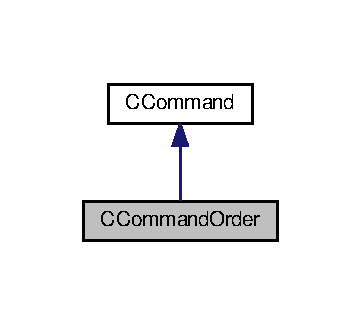
\includegraphics[width=173pt]{classCCommandOrder__coll__graph}
\end{center}
\end{figure}
\subsection*{Public Member Functions}
\begin{DoxyCompactItemize}
\item 
\hyperlink{classCCommandOrder_adaa58de546f665fd4a44ab26e7167a6c}{C\+Command\+Order} ()
\item 
\hyperlink{classCCommandOrder_a8afb685cd8016829b9f525002fc77408}{$\sim$\+C\+Command\+Order} () override=default
\item 
\hyperlink{classCCommandOrder_a669df24808e588498231b4c49536d738}{C\+Command\+Order} (string var\+Name)
\item 
bool \hyperlink{classCCommandOrder_a26192670b49e62a03d8ce240c1e2c983}{Execute} (\hyperlink{classCMemory}{C\+Memory} \&memory) override
\end{DoxyCompactItemize}
\subsection*{Public Attributes}
\begin{DoxyCompactItemize}
\item 
int \hyperlink{classCCommandOrder_ab815291bf8d2fa527a2015ce5395d64e}{m\+\_\+\+Order}
\end{DoxyCompactItemize}
\subsection*{Private Attributes}
\begin{DoxyCompactItemize}
\item 
string \hyperlink{classCCommandOrder_a45fb2d9961cefa2347113dc870bec8fb}{m\+\_\+\+Var\+Name}
\end{DoxyCompactItemize}


\subsection{Constructor \& Destructor Documentation}
\index{C\+Command\+Order@{C\+Command\+Order}!C\+Command\+Order@{C\+Command\+Order}}
\index{C\+Command\+Order@{C\+Command\+Order}!C\+Command\+Order@{C\+Command\+Order}}
\subsubsection[{\texorpdfstring{C\+Command\+Order()}{CCommandOrder()}}]{\setlength{\rightskip}{0pt plus 5cm}C\+Command\+Order\+::\+C\+Command\+Order (
\begin{DoxyParamCaption}
{}
\end{DoxyParamCaption}
)\hspace{0.3cm}{\ttfamily [inline]}}\hypertarget{classCCommandOrder_adaa58de546f665fd4a44ab26e7167a6c}{}\label{classCCommandOrder_adaa58de546f665fd4a44ab26e7167a6c}
\index{C\+Command\+Order@{C\+Command\+Order}!````~C\+Command\+Order@{$\sim$\+C\+Command\+Order}}
\index{````~C\+Command\+Order@{$\sim$\+C\+Command\+Order}!C\+Command\+Order@{C\+Command\+Order}}
\subsubsection[{\texorpdfstring{$\sim$\+C\+Command\+Order() override=default}{~CCommandOrder() override=default}}]{\setlength{\rightskip}{0pt plus 5cm}C\+Command\+Order\+::$\sim$\+C\+Command\+Order (
\begin{DoxyParamCaption}
{}
\end{DoxyParamCaption}
)\hspace{0.3cm}{\ttfamily [override]}, {\ttfamily [default]}}\hypertarget{classCCommandOrder_a8afb685cd8016829b9f525002fc77408}{}\label{classCCommandOrder_a8afb685cd8016829b9f525002fc77408}
\index{C\+Command\+Order@{C\+Command\+Order}!C\+Command\+Order@{C\+Command\+Order}}
\index{C\+Command\+Order@{C\+Command\+Order}!C\+Command\+Order@{C\+Command\+Order}}
\subsubsection[{\texorpdfstring{C\+Command\+Order(string var\+Name)}{CCommandOrder(string varName)}}]{\setlength{\rightskip}{0pt plus 5cm}C\+Command\+Order\+::\+C\+Command\+Order (
\begin{DoxyParamCaption}
\item[{string}]{var\+Name}
\end{DoxyParamCaption}
)\hspace{0.3cm}{\ttfamily [inline]}}\hypertarget{classCCommandOrder_a669df24808e588498231b4c49536d738}{}\label{classCCommandOrder_a669df24808e588498231b4c49536d738}


\subsection{Member Function Documentation}
\index{C\+Command\+Order@{C\+Command\+Order}!Execute@{Execute}}
\index{Execute@{Execute}!C\+Command\+Order@{C\+Command\+Order}}
\subsubsection[{\texorpdfstring{Execute(\+C\+Memory \&memory) override}{Execute(CMemory &memory) override}}]{\setlength{\rightskip}{0pt plus 5cm}bool C\+Command\+Order\+::\+Execute (
\begin{DoxyParamCaption}
\item[{{\bf C\+Memory} \&}]{memory}
\end{DoxyParamCaption}
)\hspace{0.3cm}{\ttfamily [inline]}, {\ttfamily [override]}, {\ttfamily [virtual]}}\hypertarget{classCCommandOrder_a26192670b49e62a03d8ce240c1e2c983}{}\label{classCCommandOrder_a26192670b49e62a03d8ce240c1e2c983}


Implements \hyperlink{classCCommand_ad9361ea814093c4ebecf22bb0a3f8b79}{C\+Command}.



\subsection{Member Data Documentation}
\index{C\+Command\+Order@{C\+Command\+Order}!m\+\_\+\+Order@{m\+\_\+\+Order}}
\index{m\+\_\+\+Order@{m\+\_\+\+Order}!C\+Command\+Order@{C\+Command\+Order}}
\subsubsection[{\texorpdfstring{m\+\_\+\+Order}{m_Order}}]{\setlength{\rightskip}{0pt plus 5cm}int C\+Command\+Order\+::m\+\_\+\+Order}\hypertarget{classCCommandOrder_ab815291bf8d2fa527a2015ce5395d64e}{}\label{classCCommandOrder_ab815291bf8d2fa527a2015ce5395d64e}
\index{C\+Command\+Order@{C\+Command\+Order}!m\+\_\+\+Var\+Name@{m\+\_\+\+Var\+Name}}
\index{m\+\_\+\+Var\+Name@{m\+\_\+\+Var\+Name}!C\+Command\+Order@{C\+Command\+Order}}
\subsubsection[{\texorpdfstring{m\+\_\+\+Var\+Name}{m_VarName}}]{\setlength{\rightskip}{0pt plus 5cm}string C\+Command\+Order\+::m\+\_\+\+Var\+Name\hspace{0.3cm}{\ttfamily [private]}}\hypertarget{classCCommandOrder_a45fb2d9961cefa2347113dc870bec8fb}{}\label{classCCommandOrder_a45fb2d9961cefa2347113dc870bec8fb}


The documentation for this class was generated from the following file\+:\begin{DoxyCompactItemize}
\item 
src/\hyperlink{CCommandOrder_8h}{C\+Command\+Order.\+h}\end{DoxyCompactItemize}

\hypertarget{classCCommandPrint}{}\section{C\+Command\+Print Class Reference}
\label{classCCommandPrint}\index{C\+Command\+Print@{C\+Command\+Print}}


{\ttfamily \#include $<$C\+Command\+Print.\+h$>$}



Inheritance diagram for C\+Command\+Print\+:\nopagebreak
\begin{figure}[H]
\begin{center}
\leavevmode
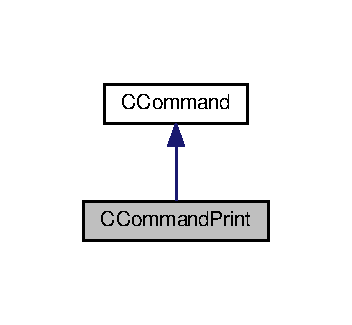
\includegraphics[width=169pt]{classCCommandPrint__inherit__graph}
\end{center}
\end{figure}


Collaboration diagram for C\+Command\+Print\+:\nopagebreak
\begin{figure}[H]
\begin{center}
\leavevmode
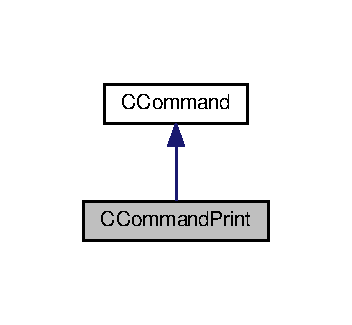
\includegraphics[width=169pt]{classCCommandPrint__coll__graph}
\end{center}
\end{figure}
\subsection*{Public Member Functions}
\begin{DoxyCompactItemize}
\item 
\hyperlink{classCCommandPrint_a3ac2095924e3b2762767d9c58a7b4718}{C\+Command\+Print} ()
\item 
\hyperlink{classCCommandPrint_add53990e292eda4fcc0908791f864ebe}{$\sim$\+C\+Command\+Print} () override=default
\item 
\hyperlink{classCCommandPrint_a064d571e6454d64271108fc9d188926e}{C\+Command\+Print} (string var\+Name)
\item 
bool \hyperlink{classCCommandPrint_afa1b192d43baa81c5ea9884972366643}{Execute} (\hyperlink{classCMemory}{C\+Memory} \&memory) override
\end{DoxyCompactItemize}
\subsection*{Private Attributes}
\begin{DoxyCompactItemize}
\item 
string \hyperlink{classCCommandPrint_a423ba460b4328ceea9ff994b4934b474}{m\+\_\+\+Variable\+Name}
\end{DoxyCompactItemize}
\subsection*{Additional Inherited Members}


\subsection{Constructor \& Destructor Documentation}
\index{C\+Command\+Print@{C\+Command\+Print}!C\+Command\+Print@{C\+Command\+Print}}
\index{C\+Command\+Print@{C\+Command\+Print}!C\+Command\+Print@{C\+Command\+Print}}
\subsubsection[{\texorpdfstring{C\+Command\+Print()}{CCommandPrint()}}]{\setlength{\rightskip}{0pt plus 5cm}C\+Command\+Print\+::\+C\+Command\+Print (
\begin{DoxyParamCaption}
{}
\end{DoxyParamCaption}
)\hspace{0.3cm}{\ttfamily [inline]}}\hypertarget{classCCommandPrint_a3ac2095924e3b2762767d9c58a7b4718}{}\label{classCCommandPrint_a3ac2095924e3b2762767d9c58a7b4718}
\index{C\+Command\+Print@{C\+Command\+Print}!````~C\+Command\+Print@{$\sim$\+C\+Command\+Print}}
\index{````~C\+Command\+Print@{$\sim$\+C\+Command\+Print}!C\+Command\+Print@{C\+Command\+Print}}
\subsubsection[{\texorpdfstring{$\sim$\+C\+Command\+Print() override=default}{~CCommandPrint() override=default}}]{\setlength{\rightskip}{0pt plus 5cm}C\+Command\+Print\+::$\sim$\+C\+Command\+Print (
\begin{DoxyParamCaption}
{}
\end{DoxyParamCaption}
)\hspace{0.3cm}{\ttfamily [override]}, {\ttfamily [default]}}\hypertarget{classCCommandPrint_add53990e292eda4fcc0908791f864ebe}{}\label{classCCommandPrint_add53990e292eda4fcc0908791f864ebe}
\index{C\+Command\+Print@{C\+Command\+Print}!C\+Command\+Print@{C\+Command\+Print}}
\index{C\+Command\+Print@{C\+Command\+Print}!C\+Command\+Print@{C\+Command\+Print}}
\subsubsection[{\texorpdfstring{C\+Command\+Print(string var\+Name)}{CCommandPrint(string varName)}}]{\setlength{\rightskip}{0pt plus 5cm}C\+Command\+Print\+::\+C\+Command\+Print (
\begin{DoxyParamCaption}
\item[{string}]{var\+Name}
\end{DoxyParamCaption}
)\hspace{0.3cm}{\ttfamily [inline]}}\hypertarget{classCCommandPrint_a064d571e6454d64271108fc9d188926e}{}\label{classCCommandPrint_a064d571e6454d64271108fc9d188926e}


\subsection{Member Function Documentation}
\index{C\+Command\+Print@{C\+Command\+Print}!Execute@{Execute}}
\index{Execute@{Execute}!C\+Command\+Print@{C\+Command\+Print}}
\subsubsection[{\texorpdfstring{Execute(\+C\+Memory \&memory) override}{Execute(CMemory &memory) override}}]{\setlength{\rightskip}{0pt plus 5cm}bool C\+Command\+Print\+::\+Execute (
\begin{DoxyParamCaption}
\item[{{\bf C\+Memory} \&}]{memory}
\end{DoxyParamCaption}
)\hspace{0.3cm}{\ttfamily [override]}, {\ttfamily [virtual]}}\hypertarget{classCCommandPrint_afa1b192d43baa81c5ea9884972366643}{}\label{classCCommandPrint_afa1b192d43baa81c5ea9884972366643}
Execute command. 
\begin{DoxyParams}{Parameters}
{\em memory} & \\
\hline
\end{DoxyParams}
\begin{DoxyReturn}{Returns}
true if execution successful, false otherwise (command cannot be performed) 
\end{DoxyReturn}


Implements \hyperlink{classCCommand_ad9361ea814093c4ebecf22bb0a3f8b79}{C\+Command}.



\subsection{Member Data Documentation}
\index{C\+Command\+Print@{C\+Command\+Print}!m\+\_\+\+Variable\+Name@{m\+\_\+\+Variable\+Name}}
\index{m\+\_\+\+Variable\+Name@{m\+\_\+\+Variable\+Name}!C\+Command\+Print@{C\+Command\+Print}}
\subsubsection[{\texorpdfstring{m\+\_\+\+Variable\+Name}{m_VariableName}}]{\setlength{\rightskip}{0pt plus 5cm}string C\+Command\+Print\+::m\+\_\+\+Variable\+Name\hspace{0.3cm}{\ttfamily [private]}}\hypertarget{classCCommandPrint_a423ba460b4328ceea9ff994b4934b474}{}\label{classCCommandPrint_a423ba460b4328ceea9ff994b4934b474}


The documentation for this class was generated from the following files\+:\begin{DoxyCompactItemize}
\item 
src/\hyperlink{CCommandPrint_8h}{C\+Command\+Print.\+h}\item 
src/\hyperlink{CCommandPrint_8cpp}{C\+Command\+Print.\+cpp}\end{DoxyCompactItemize}

\hypertarget{classCCommandPut}{}\section{C\+Command\+Put Class Reference}
\label{classCCommandPut}\index{C\+Command\+Put@{C\+Command\+Put}}


{\ttfamily \#include $<$C\+Command\+Put.\+h$>$}



Inheritance diagram for C\+Command\+Put\+:\nopagebreak
\begin{figure}[H]
\begin{center}
\leavevmode
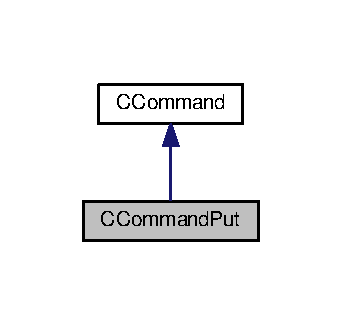
\includegraphics[width=164pt]{classCCommandPut__inherit__graph}
\end{center}
\end{figure}


Collaboration diagram for C\+Command\+Put\+:\nopagebreak
\begin{figure}[H]
\begin{center}
\leavevmode
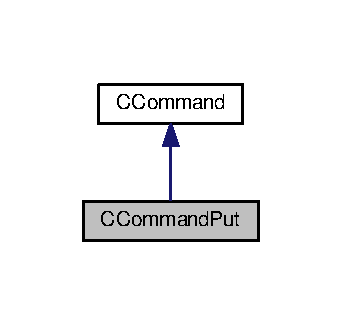
\includegraphics[width=164pt]{classCCommandPut__coll__graph}
\end{center}
\end{figure}
\subsection*{Public Member Functions}
\begin{DoxyCompactItemize}
\item 
\hyperlink{classCCommandPut_a4d53bed5af461e55b837b580ee3976a3}{C\+Command\+Put} ()
\item 
\hyperlink{classCCommandPut_a0156ac693dff6dcf0080e183b95801a3}{$\sim$\+C\+Command\+Put} () override=default
\item 
\hyperlink{classCCommandPut_aef37d51baeb780525555ff2f5e9f5c09}{C\+Command\+Put} (string var\+Name, unique\+\_\+ptr$<$ \hyperlink{classCCommand}{C\+Command} $>$ \&sub\+Command)
\item 
bool \hyperlink{classCCommandPut_a4b82c56cf3d5aafc75701ec72f8f17dc}{Execute} (\hyperlink{classCMemory}{C\+Memory} \&memory) override
\end{DoxyCompactItemize}
\subsection*{Private Attributes}
\begin{DoxyCompactItemize}
\item 
string \hyperlink{classCCommandPut_a583f3fd126a5fc69456c4538e1783f00}{m\+\_\+\+Variable\+Name}
\item 
unique\+\_\+ptr$<$ \hyperlink{classCCommand}{C\+Command} $>$ \hyperlink{classCCommandPut_abf1c7a0d0d5c112640b529ba90637d74}{m\+\_\+\+Subcommand}
\end{DoxyCompactItemize}
\subsection*{Additional Inherited Members}


\subsection{Constructor \& Destructor Documentation}
\index{C\+Command\+Put@{C\+Command\+Put}!C\+Command\+Put@{C\+Command\+Put}}
\index{C\+Command\+Put@{C\+Command\+Put}!C\+Command\+Put@{C\+Command\+Put}}
\subsubsection[{\texorpdfstring{C\+Command\+Put()}{CCommandPut()}}]{\setlength{\rightskip}{0pt plus 5cm}C\+Command\+Put\+::\+C\+Command\+Put (
\begin{DoxyParamCaption}
{}
\end{DoxyParamCaption}
)\hspace{0.3cm}{\ttfamily [inline]}}\hypertarget{classCCommandPut_a4d53bed5af461e55b837b580ee3976a3}{}\label{classCCommandPut_a4d53bed5af461e55b837b580ee3976a3}
\index{C\+Command\+Put@{C\+Command\+Put}!````~C\+Command\+Put@{$\sim$\+C\+Command\+Put}}
\index{````~C\+Command\+Put@{$\sim$\+C\+Command\+Put}!C\+Command\+Put@{C\+Command\+Put}}
\subsubsection[{\texorpdfstring{$\sim$\+C\+Command\+Put() override=default}{~CCommandPut() override=default}}]{\setlength{\rightskip}{0pt plus 5cm}C\+Command\+Put\+::$\sim$\+C\+Command\+Put (
\begin{DoxyParamCaption}
{}
\end{DoxyParamCaption}
)\hspace{0.3cm}{\ttfamily [override]}, {\ttfamily [default]}}\hypertarget{classCCommandPut_a0156ac693dff6dcf0080e183b95801a3}{}\label{classCCommandPut_a0156ac693dff6dcf0080e183b95801a3}
\index{C\+Command\+Put@{C\+Command\+Put}!C\+Command\+Put@{C\+Command\+Put}}
\index{C\+Command\+Put@{C\+Command\+Put}!C\+Command\+Put@{C\+Command\+Put}}
\subsubsection[{\texorpdfstring{C\+Command\+Put(string var\+Name, unique\+\_\+ptr$<$ C\+Command $>$ \&sub\+Command)}{CCommandPut(string varName, unique_ptr< CCommand > &subCommand)}}]{\setlength{\rightskip}{0pt plus 5cm}C\+Command\+Put\+::\+C\+Command\+Put (
\begin{DoxyParamCaption}
\item[{string}]{var\+Name, }
\item[{unique\+\_\+ptr$<$ {\bf C\+Command} $>$ \&}]{sub\+Command}
\end{DoxyParamCaption}
)\hspace{0.3cm}{\ttfamily [inline]}}\hypertarget{classCCommandPut_aef37d51baeb780525555ff2f5e9f5c09}{}\label{classCCommandPut_aef37d51baeb780525555ff2f5e9f5c09}


\subsection{Member Function Documentation}
\index{C\+Command\+Put@{C\+Command\+Put}!Execute@{Execute}}
\index{Execute@{Execute}!C\+Command\+Put@{C\+Command\+Put}}
\subsubsection[{\texorpdfstring{Execute(\+C\+Memory \&memory) override}{Execute(CMemory &memory) override}}]{\setlength{\rightskip}{0pt plus 5cm}bool C\+Command\+Put\+::\+Execute (
\begin{DoxyParamCaption}
\item[{{\bf C\+Memory} \&}]{memory}
\end{DoxyParamCaption}
)\hspace{0.3cm}{\ttfamily [override]}, {\ttfamily [virtual]}}\hypertarget{classCCommandPut_a4b82c56cf3d5aafc75701ec72f8f17dc}{}\label{classCCommandPut_a4b82c56cf3d5aafc75701ec72f8f17dc}
Execute command. 
\begin{DoxyParams}{Parameters}
{\em memory} & \\
\hline
\end{DoxyParams}
\begin{DoxyReturn}{Returns}
true if execution successful, false otherwise (command cannot be performed) 
\end{DoxyReturn}


Implements \hyperlink{classCCommand_ad9361ea814093c4ebecf22bb0a3f8b79}{C\+Command}.



\subsection{Member Data Documentation}
\index{C\+Command\+Put@{C\+Command\+Put}!m\+\_\+\+Subcommand@{m\+\_\+\+Subcommand}}
\index{m\+\_\+\+Subcommand@{m\+\_\+\+Subcommand}!C\+Command\+Put@{C\+Command\+Put}}
\subsubsection[{\texorpdfstring{m\+\_\+\+Subcommand}{m_Subcommand}}]{\setlength{\rightskip}{0pt plus 5cm}unique\+\_\+ptr$<${\bf C\+Command}$>$ C\+Command\+Put\+::m\+\_\+\+Subcommand\hspace{0.3cm}{\ttfamily [private]}}\hypertarget{classCCommandPut_abf1c7a0d0d5c112640b529ba90637d74}{}\label{classCCommandPut_abf1c7a0d0d5c112640b529ba90637d74}
\index{C\+Command\+Put@{C\+Command\+Put}!m\+\_\+\+Variable\+Name@{m\+\_\+\+Variable\+Name}}
\index{m\+\_\+\+Variable\+Name@{m\+\_\+\+Variable\+Name}!C\+Command\+Put@{C\+Command\+Put}}
\subsubsection[{\texorpdfstring{m\+\_\+\+Variable\+Name}{m_VariableName}}]{\setlength{\rightskip}{0pt plus 5cm}string C\+Command\+Put\+::m\+\_\+\+Variable\+Name\hspace{0.3cm}{\ttfamily [private]}}\hypertarget{classCCommandPut_a583f3fd126a5fc69456c4538e1783f00}{}\label{classCCommandPut_a583f3fd126a5fc69456c4538e1783f00}


The documentation for this class was generated from the following files\+:\begin{DoxyCompactItemize}
\item 
src/\hyperlink{CCommandPut_8h}{C\+Command\+Put.\+h}\item 
src/\hyperlink{CCommandPut_8cpp}{C\+Command\+Put.\+cpp}\end{DoxyCompactItemize}

\hypertarget{classCCommandSubtract}{}\section{C\+Command\+Subtract Class Reference}
\label{classCCommandSubtract}\index{C\+Command\+Subtract@{C\+Command\+Subtract}}


{\ttfamily \#include $<$C\+Command\+Subtract.\+h$>$}



Inheritance diagram for C\+Command\+Subtract\+:\nopagebreak
\begin{figure}[H]
\begin{center}
\leavevmode
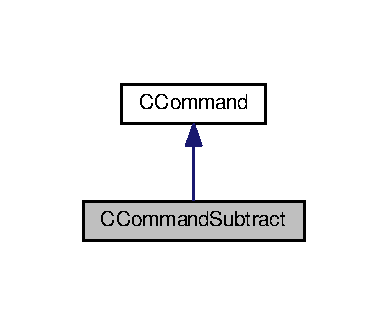
\includegraphics[width=186pt]{classCCommandSubtract__inherit__graph}
\end{center}
\end{figure}


Collaboration diagram for C\+Command\+Subtract\+:\nopagebreak
\begin{figure}[H]
\begin{center}
\leavevmode
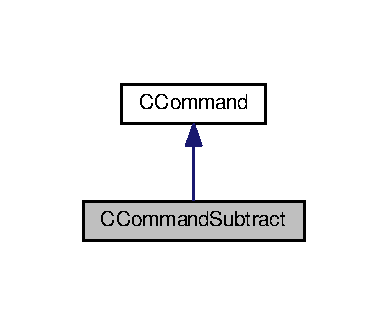
\includegraphics[width=186pt]{classCCommandSubtract__coll__graph}
\end{center}
\end{figure}
\subsection*{Public Member Functions}
\begin{DoxyCompactItemize}
\item 
\hyperlink{classCCommandSubtract_a658496963167ac339c899846fbe121aa}{C\+Command\+Subtract} ()
\item 
\hyperlink{classCCommandSubtract_afd8f13ca6aa8a5c2c06e9ef5ed726e05}{$\sim$\+C\+Command\+Subtract} () override=default
\item 
\hyperlink{classCCommandSubtract_ac89615cd1201b239e7bcaf37f50cc79c}{C\+Command\+Subtract} (string operand1, string operand2)
\item 
bool \hyperlink{classCCommandSubtract_ade3f2032aab4edce747d251e89a6398b}{Execute} (\hyperlink{classCMemory}{C\+Memory} \&memory) override
\end{DoxyCompactItemize}
\subsection*{Private Attributes}
\begin{DoxyCompactItemize}
\item 
string \hyperlink{classCCommandSubtract_ac0de4d1a69b9467aa080b8b46635d458}{m\+\_\+\+Operand1}
\item 
string \hyperlink{classCCommandSubtract_a2da0355a6682b78cb62992fbb6fba499}{m\+\_\+\+Operand2}
\end{DoxyCompactItemize}
\subsection*{Additional Inherited Members}


\subsection{Constructor \& Destructor Documentation}
\index{C\+Command\+Subtract@{C\+Command\+Subtract}!C\+Command\+Subtract@{C\+Command\+Subtract}}
\index{C\+Command\+Subtract@{C\+Command\+Subtract}!C\+Command\+Subtract@{C\+Command\+Subtract}}
\subsubsection[{\texorpdfstring{C\+Command\+Subtract()}{CCommandSubtract()}}]{\setlength{\rightskip}{0pt plus 5cm}C\+Command\+Subtract\+::\+C\+Command\+Subtract (
\begin{DoxyParamCaption}
{}
\end{DoxyParamCaption}
)\hspace{0.3cm}{\ttfamily [inline]}}\hypertarget{classCCommandSubtract_a658496963167ac339c899846fbe121aa}{}\label{classCCommandSubtract_a658496963167ac339c899846fbe121aa}
\index{C\+Command\+Subtract@{C\+Command\+Subtract}!````~C\+Command\+Subtract@{$\sim$\+C\+Command\+Subtract}}
\index{````~C\+Command\+Subtract@{$\sim$\+C\+Command\+Subtract}!C\+Command\+Subtract@{C\+Command\+Subtract}}
\subsubsection[{\texorpdfstring{$\sim$\+C\+Command\+Subtract() override=default}{~CCommandSubtract() override=default}}]{\setlength{\rightskip}{0pt plus 5cm}C\+Command\+Subtract\+::$\sim$\+C\+Command\+Subtract (
\begin{DoxyParamCaption}
{}
\end{DoxyParamCaption}
)\hspace{0.3cm}{\ttfamily [override]}, {\ttfamily [default]}}\hypertarget{classCCommandSubtract_afd8f13ca6aa8a5c2c06e9ef5ed726e05}{}\label{classCCommandSubtract_afd8f13ca6aa8a5c2c06e9ef5ed726e05}
\index{C\+Command\+Subtract@{C\+Command\+Subtract}!C\+Command\+Subtract@{C\+Command\+Subtract}}
\index{C\+Command\+Subtract@{C\+Command\+Subtract}!C\+Command\+Subtract@{C\+Command\+Subtract}}
\subsubsection[{\texorpdfstring{C\+Command\+Subtract(string operand1, string operand2)}{CCommandSubtract(string operand1, string operand2)}}]{\setlength{\rightskip}{0pt plus 5cm}C\+Command\+Subtract\+::\+C\+Command\+Subtract (
\begin{DoxyParamCaption}
\item[{string}]{operand1, }
\item[{string}]{operand2}
\end{DoxyParamCaption}
)\hspace{0.3cm}{\ttfamily [inline]}}\hypertarget{classCCommandSubtract_ac89615cd1201b239e7bcaf37f50cc79c}{}\label{classCCommandSubtract_ac89615cd1201b239e7bcaf37f50cc79c}


\subsection{Member Function Documentation}
\index{C\+Command\+Subtract@{C\+Command\+Subtract}!Execute@{Execute}}
\index{Execute@{Execute}!C\+Command\+Subtract@{C\+Command\+Subtract}}
\subsubsection[{\texorpdfstring{Execute(\+C\+Memory \&memory) override}{Execute(CMemory &memory) override}}]{\setlength{\rightskip}{0pt plus 5cm}bool C\+Command\+Subtract\+::\+Execute (
\begin{DoxyParamCaption}
\item[{{\bf C\+Memory} \&}]{memory}
\end{DoxyParamCaption}
)\hspace{0.3cm}{\ttfamily [inline]}, {\ttfamily [override]}, {\ttfamily [virtual]}}\hypertarget{classCCommandSubtract_ade3f2032aab4edce747d251e89a6398b}{}\label{classCCommandSubtract_ade3f2032aab4edce747d251e89a6398b}


Implements \hyperlink{classCCommand_ad9361ea814093c4ebecf22bb0a3f8b79}{C\+Command}.



\subsection{Member Data Documentation}
\index{C\+Command\+Subtract@{C\+Command\+Subtract}!m\+\_\+\+Operand1@{m\+\_\+\+Operand1}}
\index{m\+\_\+\+Operand1@{m\+\_\+\+Operand1}!C\+Command\+Subtract@{C\+Command\+Subtract}}
\subsubsection[{\texorpdfstring{m\+\_\+\+Operand1}{m_Operand1}}]{\setlength{\rightskip}{0pt plus 5cm}string C\+Command\+Subtract\+::m\+\_\+\+Operand1\hspace{0.3cm}{\ttfamily [private]}}\hypertarget{classCCommandSubtract_ac0de4d1a69b9467aa080b8b46635d458}{}\label{classCCommandSubtract_ac0de4d1a69b9467aa080b8b46635d458}
\index{C\+Command\+Subtract@{C\+Command\+Subtract}!m\+\_\+\+Operand2@{m\+\_\+\+Operand2}}
\index{m\+\_\+\+Operand2@{m\+\_\+\+Operand2}!C\+Command\+Subtract@{C\+Command\+Subtract}}
\subsubsection[{\texorpdfstring{m\+\_\+\+Operand2}{m_Operand2}}]{\setlength{\rightskip}{0pt plus 5cm}string C\+Command\+Subtract\+::m\+\_\+\+Operand2\hspace{0.3cm}{\ttfamily [private]}}\hypertarget{classCCommandSubtract_a2da0355a6682b78cb62992fbb6fba499}{}\label{classCCommandSubtract_a2da0355a6682b78cb62992fbb6fba499}


The documentation for this class was generated from the following file\+:\begin{DoxyCompactItemize}
\item 
src/\hyperlink{CCommandSubtract_8h}{C\+Command\+Subtract.\+h}\end{DoxyCompactItemize}

\hypertarget{classCCommandTranspose}{}\section{C\+Command\+Transpose Class Reference}
\label{classCCommandTranspose}\index{C\+Command\+Transpose@{C\+Command\+Transpose}}


{\ttfamily \#include $<$C\+Command\+Transpose.\+h$>$}



Inheritance diagram for C\+Command\+Transpose\+:
\nopagebreak
\begin{figure}[H]
\begin{center}
\leavevmode
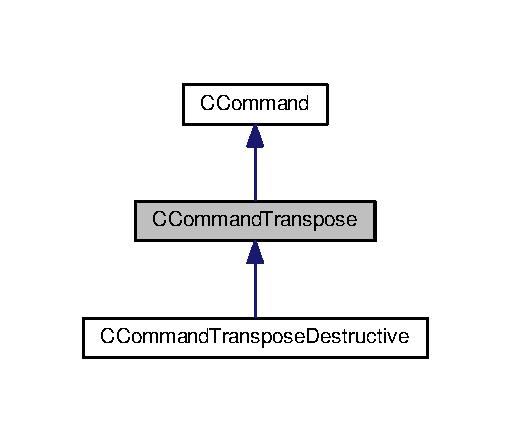
\includegraphics[width=245pt]{classCCommandTranspose__inherit__graph}
\end{center}
\end{figure}


Collaboration diagram for C\+Command\+Transpose\+:\nopagebreak
\begin{figure}[H]
\begin{center}
\leavevmode
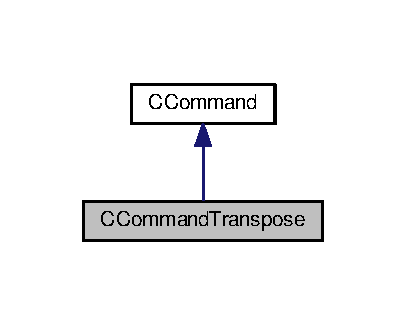
\includegraphics[width=195pt]{classCCommandTranspose__coll__graph}
\end{center}
\end{figure}
\subsection*{Public Member Functions}
\begin{DoxyCompactItemize}
\item 
\hyperlink{classCCommandTranspose_aac4a85c15491ecafd4963163b2a63670}{C\+Command\+Transpose} ()
\item 
\hyperlink{classCCommandTranspose_a5aa1525bca08133891e869631ec66144}{$\sim$\+C\+Command\+Transpose} () override=default
\item 
\hyperlink{classCCommandTranspose_ac4c0687d585f237993e679453ced64ae}{C\+Command\+Transpose} (string var\+Name)
\item 
bool \hyperlink{classCCommandTranspose_aa422d6b8bbe3efb23bcc479646392238}{Execute} (\hyperlink{classCMemory}{C\+Memory} \&memory) override
\end{DoxyCompactItemize}
\subsection*{Protected Attributes}
\begin{DoxyCompactItemize}
\item 
string \hyperlink{classCCommandTranspose_aa9eafd2768008a3f4585d65cbaa643b7}{m\+\_\+\+Var\+Name}
\end{DoxyCompactItemize}
\subsection*{Additional Inherited Members}


\subsection{Constructor \& Destructor Documentation}
\index{C\+Command\+Transpose@{C\+Command\+Transpose}!C\+Command\+Transpose@{C\+Command\+Transpose}}
\index{C\+Command\+Transpose@{C\+Command\+Transpose}!C\+Command\+Transpose@{C\+Command\+Transpose}}
\subsubsection[{\texorpdfstring{C\+Command\+Transpose()}{CCommandTranspose()}}]{\setlength{\rightskip}{0pt plus 5cm}C\+Command\+Transpose\+::\+C\+Command\+Transpose (
\begin{DoxyParamCaption}
{}
\end{DoxyParamCaption}
)\hspace{0.3cm}{\ttfamily [inline]}}\hypertarget{classCCommandTranspose_aac4a85c15491ecafd4963163b2a63670}{}\label{classCCommandTranspose_aac4a85c15491ecafd4963163b2a63670}
\index{C\+Command\+Transpose@{C\+Command\+Transpose}!````~C\+Command\+Transpose@{$\sim$\+C\+Command\+Transpose}}
\index{````~C\+Command\+Transpose@{$\sim$\+C\+Command\+Transpose}!C\+Command\+Transpose@{C\+Command\+Transpose}}
\subsubsection[{\texorpdfstring{$\sim$\+C\+Command\+Transpose() override=default}{~CCommandTranspose() override=default}}]{\setlength{\rightskip}{0pt plus 5cm}C\+Command\+Transpose\+::$\sim$\+C\+Command\+Transpose (
\begin{DoxyParamCaption}
{}
\end{DoxyParamCaption}
)\hspace{0.3cm}{\ttfamily [override]}, {\ttfamily [default]}}\hypertarget{classCCommandTranspose_a5aa1525bca08133891e869631ec66144}{}\label{classCCommandTranspose_a5aa1525bca08133891e869631ec66144}
\index{C\+Command\+Transpose@{C\+Command\+Transpose}!C\+Command\+Transpose@{C\+Command\+Transpose}}
\index{C\+Command\+Transpose@{C\+Command\+Transpose}!C\+Command\+Transpose@{C\+Command\+Transpose}}
\subsubsection[{\texorpdfstring{C\+Command\+Transpose(string var\+Name)}{CCommandTranspose(string varName)}}]{\setlength{\rightskip}{0pt plus 5cm}C\+Command\+Transpose\+::\+C\+Command\+Transpose (
\begin{DoxyParamCaption}
\item[{string}]{var\+Name}
\end{DoxyParamCaption}
)\hspace{0.3cm}{\ttfamily [inline]}}\hypertarget{classCCommandTranspose_ac4c0687d585f237993e679453ced64ae}{}\label{classCCommandTranspose_ac4c0687d585f237993e679453ced64ae}


\subsection{Member Function Documentation}
\index{C\+Command\+Transpose@{C\+Command\+Transpose}!Execute@{Execute}}
\index{Execute@{Execute}!C\+Command\+Transpose@{C\+Command\+Transpose}}
\subsubsection[{\texorpdfstring{Execute(\+C\+Memory \&memory) override}{Execute(CMemory &memory) override}}]{\setlength{\rightskip}{0pt plus 5cm}bool C\+Command\+Transpose\+::\+Execute (
\begin{DoxyParamCaption}
\item[{{\bf C\+Memory} \&}]{memory}
\end{DoxyParamCaption}
)\hspace{0.3cm}{\ttfamily [inline]}, {\ttfamily [override]}, {\ttfamily [virtual]}}\hypertarget{classCCommandTranspose_aa422d6b8bbe3efb23bcc479646392238}{}\label{classCCommandTranspose_aa422d6b8bbe3efb23bcc479646392238}


Implements \hyperlink{classCCommand_ad9361ea814093c4ebecf22bb0a3f8b79}{C\+Command}.



Reimplemented in \hyperlink{classCCommandTransposeDestructive_ae71a2b525ece1435e335f0fe496d8e87}{C\+Command\+Transpose\+Destructive}.



\subsection{Member Data Documentation}
\index{C\+Command\+Transpose@{C\+Command\+Transpose}!m\+\_\+\+Var\+Name@{m\+\_\+\+Var\+Name}}
\index{m\+\_\+\+Var\+Name@{m\+\_\+\+Var\+Name}!C\+Command\+Transpose@{C\+Command\+Transpose}}
\subsubsection[{\texorpdfstring{m\+\_\+\+Var\+Name}{m_VarName}}]{\setlength{\rightskip}{0pt plus 5cm}string C\+Command\+Transpose\+::m\+\_\+\+Var\+Name\hspace{0.3cm}{\ttfamily [protected]}}\hypertarget{classCCommandTranspose_aa9eafd2768008a3f4585d65cbaa643b7}{}\label{classCCommandTranspose_aa9eafd2768008a3f4585d65cbaa643b7}


The documentation for this class was generated from the following file\+:\begin{DoxyCompactItemize}
\item 
src/\hyperlink{CCommandTranspose_8h}{C\+Command\+Transpose.\+h}\end{DoxyCompactItemize}

\hypertarget{classCCutOperator}{}\section{C\+Cut\+Operator Class Reference}
\label{classCCutOperator}\index{C\+Cut\+Operator@{C\+Cut\+Operator}}


{\ttfamily \#include $<$C\+Cut\+Operator.\+h$>$}



Inheritance diagram for C\+Cut\+Operator\+:\nopagebreak
\begin{figure}[H]
\begin{center}
\leavevmode
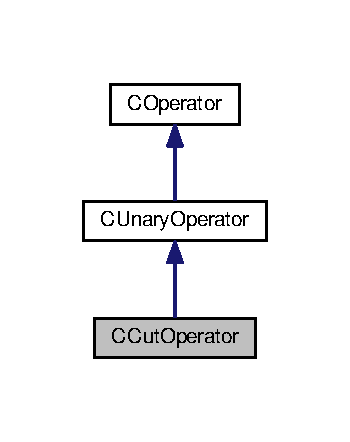
\includegraphics[width=168pt]{classCCutOperator__inherit__graph}
\end{center}
\end{figure}


Collaboration diagram for C\+Cut\+Operator\+:\nopagebreak
\begin{figure}[H]
\begin{center}
\leavevmode
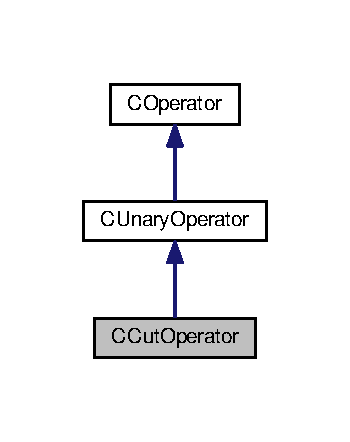
\includegraphics[width=168pt]{classCCutOperator__coll__graph}
\end{center}
\end{figure}
\subsection*{Public Member Functions}
\begin{DoxyCompactItemize}
\item 
\hyperlink{classCCutOperator_a821d6a50def27608e635434e3ca73432}{C\+Cut\+Operator} (shared\+\_\+ptr$<$ \hyperlink{classCMatrix}{C\+Matrix} $>$ \&operand, std\+::size\+\_\+t num\+Rows, std\+::size\+\_\+t num\+Cols, pair$<$ size\+\_\+t, size\+\_\+t $>$ start\+Point)
\item 
\hyperlink{classCMatrix}{C\+Matrix} $\ast$ \hyperlink{classCCutOperator_ad401b31051d8b245cc0258d773f4f816}{Evaluate} (\hyperlink{classCMemory}{C\+Memory} \&memory) override
\end{DoxyCompactItemize}
\subsection*{Private Attributes}
\begin{DoxyCompactItemize}
\item 
std\+::size\+\_\+t \hyperlink{classCCutOperator_af8d34f5712a90c9969823f75a719dc1b}{m\+\_\+\+Num\+Rows}
\item 
std\+::size\+\_\+t \hyperlink{classCCutOperator_a79665dc45c36827946d70561b17972e1}{m\+\_\+\+Num\+Cols}
\item 
pair$<$ size\+\_\+t, size\+\_\+t $>$ \hyperlink{classCCutOperator_aa58b7138e83bd58cc64f8fac3325ce80}{m\+\_\+\+Start\+Point}
\end{DoxyCompactItemize}
\subsection*{Additional Inherited Members}


\subsection{Constructor \& Destructor Documentation}
\index{C\+Cut\+Operator@{C\+Cut\+Operator}!C\+Cut\+Operator@{C\+Cut\+Operator}}
\index{C\+Cut\+Operator@{C\+Cut\+Operator}!C\+Cut\+Operator@{C\+Cut\+Operator}}
\subsubsection[{\texorpdfstring{C\+Cut\+Operator(shared\+\_\+ptr$<$ C\+Matrix $>$ \&operand, std\+::size\+\_\+t num\+Rows, std\+::size\+\_\+t num\+Cols, pair$<$ size\+\_\+t, size\+\_\+t $>$ start\+Point)}{CCutOperator(shared_ptr< CMatrix > &operand, std::size_t numRows, std::size_t numCols, pair< size_t, size_t > startPoint)}}]{\setlength{\rightskip}{0pt plus 5cm}C\+Cut\+Operator\+::\+C\+Cut\+Operator (
\begin{DoxyParamCaption}
\item[{shared\+\_\+ptr$<$ {\bf C\+Matrix} $>$ \&}]{operand, }
\item[{std\+::size\+\_\+t}]{num\+Rows, }
\item[{std\+::size\+\_\+t}]{num\+Cols, }
\item[{pair$<$ size\+\_\+t, size\+\_\+t $>$}]{start\+Point}
\end{DoxyParamCaption}
)\hspace{0.3cm}{\ttfamily [inline]}}\hypertarget{classCCutOperator_a821d6a50def27608e635434e3ca73432}{}\label{classCCutOperator_a821d6a50def27608e635434e3ca73432}


\subsection{Member Function Documentation}
\index{C\+Cut\+Operator@{C\+Cut\+Operator}!Evaluate@{Evaluate}}
\index{Evaluate@{Evaluate}!C\+Cut\+Operator@{C\+Cut\+Operator}}
\subsubsection[{\texorpdfstring{Evaluate(\+C\+Memory \&memory) override}{Evaluate(CMemory &memory) override}}]{\setlength{\rightskip}{0pt plus 5cm}{\bf C\+Matrix} $\ast$ C\+Cut\+Operator\+::\+Evaluate (
\begin{DoxyParamCaption}
\item[{{\bf C\+Memory} \&}]{memory}
\end{DoxyParamCaption}
)\hspace{0.3cm}{\ttfamily [override]}, {\ttfamily [virtual]}}\hypertarget{classCCutOperator_ad401b31051d8b245cc0258d773f4f816}{}\label{classCCutOperator_ad401b31051d8b245cc0258d773f4f816}
Cut matrix according to parameters. 

Implements \hyperlink{classCUnaryOperator_a17b01d9de023a58642f6fd82f214cde0}{C\+Unary\+Operator}.



\subsection{Member Data Documentation}
\index{C\+Cut\+Operator@{C\+Cut\+Operator}!m\+\_\+\+Num\+Cols@{m\+\_\+\+Num\+Cols}}
\index{m\+\_\+\+Num\+Cols@{m\+\_\+\+Num\+Cols}!C\+Cut\+Operator@{C\+Cut\+Operator}}
\subsubsection[{\texorpdfstring{m\+\_\+\+Num\+Cols}{m_NumCols}}]{\setlength{\rightskip}{0pt plus 5cm}std\+::size\+\_\+t C\+Cut\+Operator\+::m\+\_\+\+Num\+Cols\hspace{0.3cm}{\ttfamily [private]}}\hypertarget{classCCutOperator_a79665dc45c36827946d70561b17972e1}{}\label{classCCutOperator_a79665dc45c36827946d70561b17972e1}
\index{C\+Cut\+Operator@{C\+Cut\+Operator}!m\+\_\+\+Num\+Rows@{m\+\_\+\+Num\+Rows}}
\index{m\+\_\+\+Num\+Rows@{m\+\_\+\+Num\+Rows}!C\+Cut\+Operator@{C\+Cut\+Operator}}
\subsubsection[{\texorpdfstring{m\+\_\+\+Num\+Rows}{m_NumRows}}]{\setlength{\rightskip}{0pt plus 5cm}std\+::size\+\_\+t C\+Cut\+Operator\+::m\+\_\+\+Num\+Rows\hspace{0.3cm}{\ttfamily [private]}}\hypertarget{classCCutOperator_af8d34f5712a90c9969823f75a719dc1b}{}\label{classCCutOperator_af8d34f5712a90c9969823f75a719dc1b}
\index{C\+Cut\+Operator@{C\+Cut\+Operator}!m\+\_\+\+Start\+Point@{m\+\_\+\+Start\+Point}}
\index{m\+\_\+\+Start\+Point@{m\+\_\+\+Start\+Point}!C\+Cut\+Operator@{C\+Cut\+Operator}}
\subsubsection[{\texorpdfstring{m\+\_\+\+Start\+Point}{m_StartPoint}}]{\setlength{\rightskip}{0pt plus 5cm}pair$<$size\+\_\+t, size\+\_\+t$>$ C\+Cut\+Operator\+::m\+\_\+\+Start\+Point\hspace{0.3cm}{\ttfamily [private]}}\hypertarget{classCCutOperator_aa58b7138e83bd58cc64f8fac3325ce80}{}\label{classCCutOperator_aa58b7138e83bd58cc64f8fac3325ce80}


The documentation for this class was generated from the following files\+:\begin{DoxyCompactItemize}
\item 
src/\hyperlink{CCutOperator_8h}{C\+Cut\+Operator.\+h}\item 
src/\hyperlink{CCutOperator_8cpp}{C\+Cut\+Operator.\+cpp}\end{DoxyCompactItemize}

\hypertarget{classCDeterminantCalculator}{}\section{C\+Determinant\+Calculator Class Reference}
\label{classCDeterminantCalculator}\index{C\+Determinant\+Calculator@{C\+Determinant\+Calculator}}


{\ttfamily \#include $<$C\+Determinant\+Calculator.\+h$>$}

\subsection*{Public Member Functions}
\begin{DoxyCompactItemize}
\item 
double \hyperlink{classCDeterminantCalculator_a1f86ba4955b9cabf3042b96be7563a10}{operator()} (const shared\+\_\+ptr$<$ \hyperlink{classCMatrix}{C\+Matrix} $>$ \&matrix)
\end{DoxyCompactItemize}
\subsection*{Private Member Functions}
\begin{DoxyCompactItemize}
\item 
double \hyperlink{classCDeterminantCalculator_a1b56e8907eb6d7bbc9083d7f10118186}{Calculate\+Determinant} (shared\+\_\+ptr$<$ \hyperlink{classCMatrix}{C\+Matrix} $>$ \&matrix)
\item 
void \hyperlink{classCDeterminantCalculator_a9da30150339c152a64e7e43b10d98d08}{Add\+Diagonal} (double \&det, shared\+\_\+ptr$<$ \hyperlink{classCMatrix}{C\+Matrix} $>$ \&matrix) const 
\end{DoxyCompactItemize}
\subsection*{Static Private Member Functions}
\begin{DoxyCompactItemize}
\item 
static bool \hyperlink{classCDeterminantCalculator_a3cda3c851df4a12fa39cef7b5fe08261}{Has\+Zero\+Row\+Or\+Col} (const shared\+\_\+ptr$<$ \hyperlink{classCMatrix}{C\+Matrix} $>$ \&matrix)
\end{DoxyCompactItemize}


\subsection{Member Function Documentation}
\index{C\+Determinant\+Calculator@{C\+Determinant\+Calculator}!Add\+Diagonal@{Add\+Diagonal}}
\index{Add\+Diagonal@{Add\+Diagonal}!C\+Determinant\+Calculator@{C\+Determinant\+Calculator}}
\subsubsection[{\texorpdfstring{Add\+Diagonal(double \&det, shared\+\_\+ptr$<$ C\+Matrix $>$ \&matrix) const }{AddDiagonal(double &det, shared_ptr< CMatrix > &matrix) const }}]{\setlength{\rightskip}{0pt plus 5cm}void C\+Determinant\+Calculator\+::\+Add\+Diagonal (
\begin{DoxyParamCaption}
\item[{double \&}]{det, }
\item[{shared\+\_\+ptr$<$ {\bf C\+Matrix} $>$ \&}]{matrix}
\end{DoxyParamCaption}
) const\hspace{0.3cm}{\ttfamily [inline]}, {\ttfamily [private]}}\hypertarget{classCDeterminantCalculator_a9da30150339c152a64e7e43b10d98d08}{}\label{classCDeterminantCalculator_a9da30150339c152a64e7e43b10d98d08}
Multiply diagonal values of a square matrix. 
\begin{DoxyParams}{Parameters}
{\em det} & \\
\hline
{\em matrix} & \\
\hline
\end{DoxyParams}
\index{C\+Determinant\+Calculator@{C\+Determinant\+Calculator}!Calculate\+Determinant@{Calculate\+Determinant}}
\index{Calculate\+Determinant@{Calculate\+Determinant}!C\+Determinant\+Calculator@{C\+Determinant\+Calculator}}
\subsubsection[{\texorpdfstring{Calculate\+Determinant(shared\+\_\+ptr$<$ C\+Matrix $>$ \&matrix)}{CalculateDeterminant(shared_ptr< CMatrix > &matrix)}}]{\setlength{\rightskip}{0pt plus 5cm}double C\+Determinant\+Calculator\+::\+Calculate\+Determinant (
\begin{DoxyParamCaption}
\item[{shared\+\_\+ptr$<$ {\bf C\+Matrix} $>$ \&}]{matrix}
\end{DoxyParamCaption}
)\hspace{0.3cm}{\ttfamily [inline]}, {\ttfamily [private]}}\hypertarget{classCDeterminantCalculator_a1b56e8907eb6d7bbc9083d7f10118186}{}\label{classCDeterminantCalculator_a1b56e8907eb6d7bbc9083d7f10118186}
Calculate determinant by converting matrix to lower upper triangular form. 
\begin{DoxyParams}{Parameters}
{\em matrix} & matrix to have determinant calculated \\
\hline
\end{DoxyParams}
\begin{DoxyReturn}{Returns}
determinant 
\end{DoxyReturn}
\index{C\+Determinant\+Calculator@{C\+Determinant\+Calculator}!Has\+Zero\+Row\+Or\+Col@{Has\+Zero\+Row\+Or\+Col}}
\index{Has\+Zero\+Row\+Or\+Col@{Has\+Zero\+Row\+Or\+Col}!C\+Determinant\+Calculator@{C\+Determinant\+Calculator}}
\subsubsection[{\texorpdfstring{Has\+Zero\+Row\+Or\+Col(const shared\+\_\+ptr$<$ C\+Matrix $>$ \&matrix)}{HasZeroRowOrCol(const shared_ptr< CMatrix > &matrix)}}]{\setlength{\rightskip}{0pt plus 5cm}static bool C\+Determinant\+Calculator\+::\+Has\+Zero\+Row\+Or\+Col (
\begin{DoxyParamCaption}
\item[{const shared\+\_\+ptr$<$ {\bf C\+Matrix} $>$ \&}]{matrix}
\end{DoxyParamCaption}
)\hspace{0.3cm}{\ttfamily [inline]}, {\ttfamily [static]}, {\ttfamily [private]}}\hypertarget{classCDeterminantCalculator_a3cda3c851df4a12fa39cef7b5fe08261}{}\label{classCDeterminantCalculator_a3cda3c851df4a12fa39cef7b5fe08261}
Check if matrix has a row or a column with only zeroes. 
\begin{DoxyParams}{Parameters}
{\em matrix} & input matrix \\
\hline
\end{DoxyParams}
\begin{DoxyReturn}{Returns}
true if has only zero row or column, false otherwise 
\end{DoxyReturn}
\index{C\+Determinant\+Calculator@{C\+Determinant\+Calculator}!operator()@{operator()}}
\index{operator()@{operator()}!C\+Determinant\+Calculator@{C\+Determinant\+Calculator}}
\subsubsection[{\texorpdfstring{operator()(const shared\+\_\+ptr$<$ C\+Matrix $>$ \&matrix)}{operator()(const shared_ptr< CMatrix > &matrix)}}]{\setlength{\rightskip}{0pt plus 5cm}double C\+Determinant\+Calculator\+::operator() (
\begin{DoxyParamCaption}
\item[{const shared\+\_\+ptr$<$ {\bf C\+Matrix} $>$ \&}]{matrix}
\end{DoxyParamCaption}
)\hspace{0.3cm}{\ttfamily [inline]}}\hypertarget{classCDeterminantCalculator_a1f86ba4955b9cabf3042b96be7563a10}{}\label{classCDeterminantCalculator_a1f86ba4955b9cabf3042b96be7563a10}
Calculate determinant of a matrix. 
\begin{DoxyParams}{Parameters}
{\em matrix} & matrix to have determinant calculated \\
\hline
\end{DoxyParams}
\begin{DoxyReturn}{Returns}
determinant 
\end{DoxyReturn}


The documentation for this class was generated from the following file\+:\begin{DoxyCompactItemize}
\item 
src/\hyperlink{CDeterminantCalculator_8h}{C\+Determinant\+Calculator.\+h}\end{DoxyCompactItemize}

\hypertarget{classCGaussEliminationOperator}{}\section{C\+Gauss\+Elimination\+Operator Class Reference}
\label{classCGaussEliminationOperator}\index{C\+Gauss\+Elimination\+Operator@{C\+Gauss\+Elimination\+Operator}}


{\ttfamily \#include $<$C\+Gauss\+Elimination\+Operator.\+h$>$}



Inheritance diagram for C\+Gauss\+Elimination\+Operator\+:\nopagebreak
\begin{figure}[H]
\begin{center}
\leavevmode
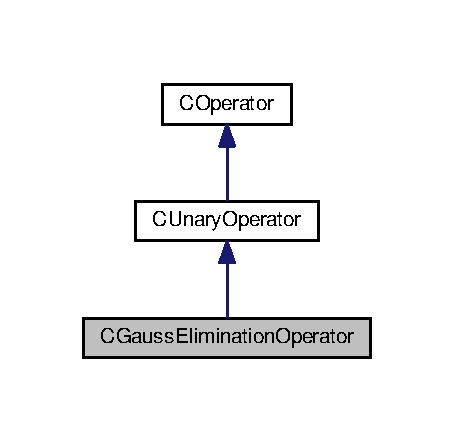
\includegraphics[width=218pt]{classCGaussEliminationOperator__inherit__graph}
\end{center}
\end{figure}


Collaboration diagram for C\+Gauss\+Elimination\+Operator\+:\nopagebreak
\begin{figure}[H]
\begin{center}
\leavevmode
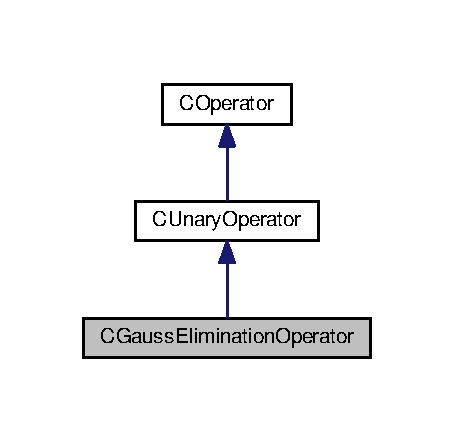
\includegraphics[width=218pt]{classCGaussEliminationOperator__coll__graph}
\end{center}
\end{figure}
\subsection*{Public Member Functions}
\begin{DoxyCompactItemize}
\item 
\hyperlink{classCGaussEliminationOperator_ad73c40a7b947e08b5d7cf294325e4d8e}{C\+Gauss\+Elimination\+Operator} (shared\+\_\+ptr$<$ \hyperlink{classCMatrix}{C\+Matrix} $>$ \&operand)
\item 
\hyperlink{classCMatrix}{C\+Matrix} $\ast$ \hyperlink{classCGaussEliminationOperator_a65b706ae08cef92db1e5aed380e1a7ee}{Evaluate} (\hyperlink{classCMemory}{C\+Memory} \&memory) override
\item 
vector$<$ shared\+\_\+ptr$<$ \hyperlink{classCMatrix}{C\+Matrix} $>$ $>$ \hyperlink{classCGaussEliminationOperator_a44b0cb343e17a349d4cb0361f1d16d97}{Get\+Elimination\+Process} ()
\end{DoxyCompactItemize}
\subsection*{Private Attributes}
\begin{DoxyCompactItemize}
\item 
vector$<$ shared\+\_\+ptr$<$ \hyperlink{classCMatrix}{C\+Matrix} $>$ $>$ \hyperlink{classCGaussEliminationOperator_ab0e40cf3182ecc239ff1bcae10e4430e}{m\+\_\+\+Elimination\+Process}
\end{DoxyCompactItemize}
\subsection*{Additional Inherited Members}


\subsection{Constructor \& Destructor Documentation}
\index{C\+Gauss\+Elimination\+Operator@{C\+Gauss\+Elimination\+Operator}!C\+Gauss\+Elimination\+Operator@{C\+Gauss\+Elimination\+Operator}}
\index{C\+Gauss\+Elimination\+Operator@{C\+Gauss\+Elimination\+Operator}!C\+Gauss\+Elimination\+Operator@{C\+Gauss\+Elimination\+Operator}}
\subsubsection[{\texorpdfstring{C\+Gauss\+Elimination\+Operator(shared\+\_\+ptr$<$ C\+Matrix $>$ \&operand)}{CGaussEliminationOperator(shared_ptr< CMatrix > &operand)}}]{\setlength{\rightskip}{0pt plus 5cm}C\+Gauss\+Elimination\+Operator\+::\+C\+Gauss\+Elimination\+Operator (
\begin{DoxyParamCaption}
\item[{shared\+\_\+ptr$<$ {\bf C\+Matrix} $>$ \&}]{operand}
\end{DoxyParamCaption}
)\hspace{0.3cm}{\ttfamily [inline]}}\hypertarget{classCGaussEliminationOperator_ad73c40a7b947e08b5d7cf294325e4d8e}{}\label{classCGaussEliminationOperator_ad73c40a7b947e08b5d7cf294325e4d8e}


\subsection{Member Function Documentation}
\index{C\+Gauss\+Elimination\+Operator@{C\+Gauss\+Elimination\+Operator}!Evaluate@{Evaluate}}
\index{Evaluate@{Evaluate}!C\+Gauss\+Elimination\+Operator@{C\+Gauss\+Elimination\+Operator}}
\subsubsection[{\texorpdfstring{Evaluate(\+C\+Memory \&memory) override}{Evaluate(CMemory &memory) override}}]{\setlength{\rightskip}{0pt plus 5cm}{\bf C\+Matrix} $\ast$ C\+Gauss\+Elimination\+Operator\+::\+Evaluate (
\begin{DoxyParamCaption}
\item[{{\bf C\+Memory} \&}]{memory}
\end{DoxyParamCaption}
)\hspace{0.3cm}{\ttfamily [override]}, {\ttfamily [virtual]}}\hypertarget{classCGaussEliminationOperator_a65b706ae08cef92db1e5aed380e1a7ee}{}\label{classCGaussEliminationOperator_a65b706ae08cef92db1e5aed380e1a7ee}
Transform variable to upper triangular form. 

Implements \hyperlink{classCUnaryOperator_a17b01d9de023a58642f6fd82f214cde0}{C\+Unary\+Operator}.

\index{C\+Gauss\+Elimination\+Operator@{C\+Gauss\+Elimination\+Operator}!Get\+Elimination\+Process@{Get\+Elimination\+Process}}
\index{Get\+Elimination\+Process@{Get\+Elimination\+Process}!C\+Gauss\+Elimination\+Operator@{C\+Gauss\+Elimination\+Operator}}
\subsubsection[{\texorpdfstring{Get\+Elimination\+Process()}{GetEliminationProcess()}}]{\setlength{\rightskip}{0pt plus 5cm}vector$<$shared\+\_\+ptr$<${\bf C\+Matrix}$>$ $>$ C\+Gauss\+Elimination\+Operator\+::\+Get\+Elimination\+Process (
\begin{DoxyParamCaption}
{}
\end{DoxyParamCaption}
)\hspace{0.3cm}{\ttfamily [inline]}}\hypertarget{classCGaussEliminationOperator_a44b0cb343e17a349d4cb0361f1d16d97}{}\label{classCGaussEliminationOperator_a44b0cb343e17a349d4cb0361f1d16d97}
Get matrices from each step of elimination process. \begin{DoxyReturn}{Returns}
vector of matrices 
\end{DoxyReturn}


\subsection{Member Data Documentation}
\index{C\+Gauss\+Elimination\+Operator@{C\+Gauss\+Elimination\+Operator}!m\+\_\+\+Elimination\+Process@{m\+\_\+\+Elimination\+Process}}
\index{m\+\_\+\+Elimination\+Process@{m\+\_\+\+Elimination\+Process}!C\+Gauss\+Elimination\+Operator@{C\+Gauss\+Elimination\+Operator}}
\subsubsection[{\texorpdfstring{m\+\_\+\+Elimination\+Process}{m_EliminationProcess}}]{\setlength{\rightskip}{0pt plus 5cm}vector$<$shared\+\_\+ptr$<${\bf C\+Matrix}$>$ $>$ C\+Gauss\+Elimination\+Operator\+::m\+\_\+\+Elimination\+Process\hspace{0.3cm}{\ttfamily [private]}}\hypertarget{classCGaussEliminationOperator_ab0e40cf3182ecc239ff1bcae10e4430e}{}\label{classCGaussEliminationOperator_ab0e40cf3182ecc239ff1bcae10e4430e}


The documentation for this class was generated from the following files\+:\begin{DoxyCompactItemize}
\item 
src/\hyperlink{CGaussEliminationOperator_8h}{C\+Gauss\+Elimination\+Operator.\+h}\item 
src/\hyperlink{CGaussEliminationOperator_8cpp}{C\+Gauss\+Elimination\+Operator.\+cpp}\end{DoxyCompactItemize}

\hypertarget{classCInverseOperator}{}\section{C\+Inverse\+Operator Class Reference}
\label{classCInverseOperator}\index{C\+Inverse\+Operator@{C\+Inverse\+Operator}}


{\ttfamily \#include $<$C\+Inverse\+Operator.\+h$>$}



Inheritance diagram for C\+Inverse\+Operator\+:\nopagebreak
\begin{figure}[H]
\begin{center}
\leavevmode
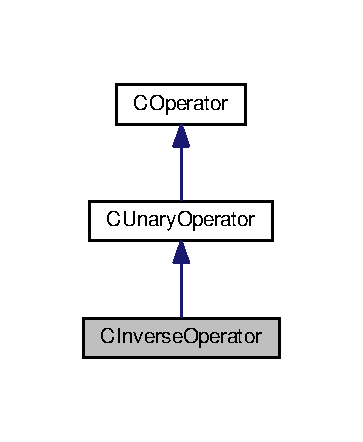
\includegraphics[width=174pt]{classCInverseOperator__inherit__graph}
\end{center}
\end{figure}


Collaboration diagram for C\+Inverse\+Operator\+:\nopagebreak
\begin{figure}[H]
\begin{center}
\leavevmode
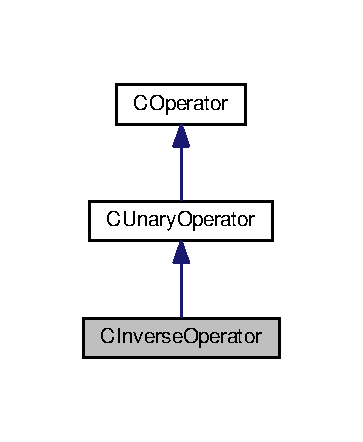
\includegraphics[width=174pt]{classCInverseOperator__coll__graph}
\end{center}
\end{figure}
\subsection*{Public Member Functions}
\begin{DoxyCompactItemize}
\item 
\hyperlink{classCInverseOperator_a67ce2e314397c4cc033963956e1284c4}{C\+Inverse\+Operator} (shared\+\_\+ptr$<$ \hyperlink{classCMatrix}{C\+Matrix} $>$ \&operand)
\item 
\hyperlink{classCMatrixStandard}{C\+Matrix\+Standard} $\ast$ \hyperlink{classCInverseOperator_a007fc0315502d838a79e83e0d2379083}{Get\+Identity} (std\+::size\+\_\+t dimension) const 
\item 
void \hyperlink{classCInverseOperator_a061d632bb989d6cf75e0f08120e22e03}{Create\+Zero\+Triangles} (shared\+\_\+ptr$<$ \hyperlink{classCMatrix}{C\+Matrix} $>$ \&matrix)
\item 
void \hyperlink{classCInverseOperator_accadb5f47ca24653afdfc77e76c7d344}{Make\+Diagonals\+To1} (shared\+\_\+ptr$<$ \hyperlink{classCMatrix}{C\+Matrix} $>$ \&matrix)
\item 
void \hyperlink{classCInverseOperator_ad931eb04b739afe11d45b05e09f760ab}{Convert\+To\+LU} (shared\+\_\+ptr$<$ \hyperlink{classCMatrix}{C\+Matrix} $>$ \&matrix)
\item 
\hyperlink{classCMatrix}{C\+Matrix} $\ast$ \hyperlink{classCInverseOperator_a72d6bb822dcc0d7944c9aaf53fa62b9f}{Evaluate} (\hyperlink{classCMemory}{C\+Memory} \&memory) override
\end{DoxyCompactItemize}
\subsection*{Additional Inherited Members}


\subsection{Constructor \& Destructor Documentation}
\index{C\+Inverse\+Operator@{C\+Inverse\+Operator}!C\+Inverse\+Operator@{C\+Inverse\+Operator}}
\index{C\+Inverse\+Operator@{C\+Inverse\+Operator}!C\+Inverse\+Operator@{C\+Inverse\+Operator}}
\subsubsection[{\texorpdfstring{C\+Inverse\+Operator(shared\+\_\+ptr$<$ C\+Matrix $>$ \&operand)}{CInverseOperator(shared_ptr< CMatrix > &operand)}}]{\setlength{\rightskip}{0pt plus 5cm}C\+Inverse\+Operator\+::\+C\+Inverse\+Operator (
\begin{DoxyParamCaption}
\item[{shared\+\_\+ptr$<$ {\bf C\+Matrix} $>$ \&}]{operand}
\end{DoxyParamCaption}
)\hspace{0.3cm}{\ttfamily [inline]}}\hypertarget{classCInverseOperator_a67ce2e314397c4cc033963956e1284c4}{}\label{classCInverseOperator_a67ce2e314397c4cc033963956e1284c4}


\subsection{Member Function Documentation}
\index{C\+Inverse\+Operator@{C\+Inverse\+Operator}!Convert\+To\+LU@{Convert\+To\+LU}}
\index{Convert\+To\+LU@{Convert\+To\+LU}!C\+Inverse\+Operator@{C\+Inverse\+Operator}}
\subsubsection[{\texorpdfstring{Convert\+To\+L\+U(shared\+\_\+ptr$<$ C\+Matrix $>$ \&matrix)}{ConvertToLU(shared_ptr< CMatrix > &matrix)}}]{\setlength{\rightskip}{0pt plus 5cm}void C\+Inverse\+Operator\+::\+Convert\+To\+LU (
\begin{DoxyParamCaption}
\item[{shared\+\_\+ptr$<$ {\bf C\+Matrix} $>$ \&}]{matrix}
\end{DoxyParamCaption}
)\hspace{0.3cm}{\ttfamily [inline]}}\hypertarget{classCInverseOperator_ad931eb04b739afe11d45b05e09f760ab}{}\label{classCInverseOperator_ad931eb04b739afe11d45b05e09f760ab}
Convert augumented matrix so that it begins with an identity matrix. 
\begin{DoxyParams}{Parameters}
{\em matrix} & matrix to be converted \\
\hline
\end{DoxyParams}
\index{C\+Inverse\+Operator@{C\+Inverse\+Operator}!Create\+Zero\+Triangles@{Create\+Zero\+Triangles}}
\index{Create\+Zero\+Triangles@{Create\+Zero\+Triangles}!C\+Inverse\+Operator@{C\+Inverse\+Operator}}
\subsubsection[{\texorpdfstring{Create\+Zero\+Triangles(shared\+\_\+ptr$<$ C\+Matrix $>$ \&matrix)}{CreateZeroTriangles(shared_ptr< CMatrix > &matrix)}}]{\setlength{\rightskip}{0pt plus 5cm}void C\+Inverse\+Operator\+::\+Create\+Zero\+Triangles (
\begin{DoxyParamCaption}
\item[{shared\+\_\+ptr$<$ {\bf C\+Matrix} $>$ \&}]{matrix}
\end{DoxyParamCaption}
)\hspace{0.3cm}{\ttfamily [inline]}}\hypertarget{classCInverseOperator_a061d632bb989d6cf75e0f08120e22e03}{}\label{classCInverseOperator_a061d632bb989d6cf75e0f08120e22e03}
Convert augumented matrix so that it begins with a square matrix in lower upper triangular form (diagonal). 
\begin{DoxyParams}{Parameters}
{\em matrix} & matrix to be converted \\
\hline
\end{DoxyParams}
\index{C\+Inverse\+Operator@{C\+Inverse\+Operator}!Evaluate@{Evaluate}}
\index{Evaluate@{Evaluate}!C\+Inverse\+Operator@{C\+Inverse\+Operator}}
\subsubsection[{\texorpdfstring{Evaluate(\+C\+Memory \&memory) override}{Evaluate(CMemory &memory) override}}]{\setlength{\rightskip}{0pt plus 5cm}{\bf C\+Matrix}$\ast$ C\+Inverse\+Operator\+::\+Evaluate (
\begin{DoxyParamCaption}
\item[{{\bf C\+Memory} \&}]{memory}
\end{DoxyParamCaption}
)\hspace{0.3cm}{\ttfamily [inline]}, {\ttfamily [override]}, {\ttfamily [virtual]}}\hypertarget{classCInverseOperator_a72d6bb822dcc0d7944c9aaf53fa62b9f}{}\label{classCInverseOperator_a72d6bb822dcc0d7944c9aaf53fa62b9f}
Find inverse of a variable. 

Implements \hyperlink{classCUnaryOperator_a17b01d9de023a58642f6fd82f214cde0}{C\+Unary\+Operator}.

\index{C\+Inverse\+Operator@{C\+Inverse\+Operator}!Get\+Identity@{Get\+Identity}}
\index{Get\+Identity@{Get\+Identity}!C\+Inverse\+Operator@{C\+Inverse\+Operator}}
\subsubsection[{\texorpdfstring{Get\+Identity(std\+::size\+\_\+t dimension) const }{GetIdentity(std::size_t dimension) const }}]{\setlength{\rightskip}{0pt plus 5cm}{\bf C\+Matrix\+Standard}$\ast$ C\+Inverse\+Operator\+::\+Get\+Identity (
\begin{DoxyParamCaption}
\item[{std\+::size\+\_\+t}]{dimension}
\end{DoxyParamCaption}
) const\hspace{0.3cm}{\ttfamily [inline]}}\hypertarget{classCInverseOperator_a007fc0315502d838a79e83e0d2379083}{}\label{classCInverseOperator_a007fc0315502d838a79e83e0d2379083}
Get new identity matrix. 
\begin{DoxyParams}{Parameters}
{\em dimension} & size of matrix to be created \\
\hline
\end{DoxyParams}
\begin{DoxyReturn}{Returns}
new identity matrix 
\end{DoxyReturn}
\index{C\+Inverse\+Operator@{C\+Inverse\+Operator}!Make\+Diagonals\+To1@{Make\+Diagonals\+To1}}
\index{Make\+Diagonals\+To1@{Make\+Diagonals\+To1}!C\+Inverse\+Operator@{C\+Inverse\+Operator}}
\subsubsection[{\texorpdfstring{Make\+Diagonals\+To1(shared\+\_\+ptr$<$ C\+Matrix $>$ \&matrix)}{MakeDiagonalsTo1(shared_ptr< CMatrix > &matrix)}}]{\setlength{\rightskip}{0pt plus 5cm}void C\+Inverse\+Operator\+::\+Make\+Diagonals\+To1 (
\begin{DoxyParamCaption}
\item[{shared\+\_\+ptr$<$ {\bf C\+Matrix} $>$ \&}]{matrix}
\end{DoxyParamCaption}
)\hspace{0.3cm}{\ttfamily [inline]}}\hypertarget{classCInverseOperator_accadb5f47ca24653afdfc77e76c7d344}{}\label{classCInverseOperator_accadb5f47ca24653afdfc77e76c7d344}
Make diagonal of beginning square matrix of augumented matrix to 1. Each row is divided by number on the diagonal of the beginning square matrix. 
\begin{DoxyParams}{Parameters}
{\em matrix} & augumented matrix to be converted \\
\hline
\end{DoxyParams}


The documentation for this class was generated from the following file\+:\begin{DoxyCompactItemize}
\item 
src/\hyperlink{CInverseOperator_8h}{C\+Inverse\+Operator.\+h}\end{DoxyCompactItemize}

\hypertarget{classCMatrix}{}\section{C\+Matrix Class Reference}
\label{classCMatrix}\index{C\+Matrix@{C\+Matrix}}


{\ttfamily \#include $<$C\+Matrix.\+h$>$}



Inheritance diagram for C\+Matrix\+:\nopagebreak
\begin{figure}[H]
\begin{center}
\leavevmode
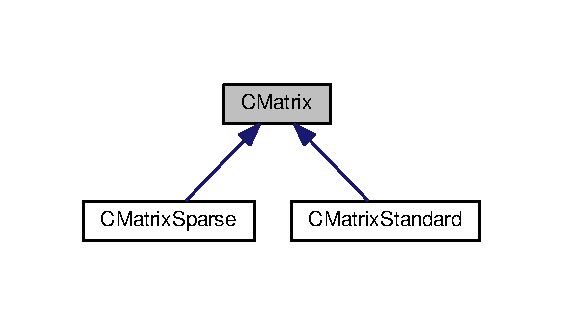
\includegraphics[width=270pt]{classCMatrix__inherit__graph}
\end{center}
\end{figure}
\subsection*{Public Member Functions}
\begin{DoxyCompactItemize}
\item 
\hyperlink{classCMatrix_ab91da59b03ce55dc412bc69578ecc855}{C\+Matrix} ()=default
\item 
virtual \hyperlink{classCMatrix_a0c4bbe807ddb1122065db4c3e3d6f964}{$\sim$\+C\+Matrix} ()=default
\item 
virtual void \hyperlink{classCMatrix_a424a048d20918f0f041f4a8645823ae7}{Print} () const =0
\item 
virtual double \hyperlink{classCMatrix_afa0213e0a6c5823e6b6e786891cc5f2d}{Get\+Num\+At\+Coords} (size\+\_\+t row, size\+\_\+t col) const =0
\item 
virtual void \hyperlink{classCMatrix_afeba0f7cfcc2623bde41cf6111b0ef6a}{Set\+Num\+At\+Coords} (size\+\_\+t row, size\+\_\+t col, double value)=0
\item 
virtual \hyperlink{classCMatrix}{C\+Matrix} $\ast$ \hyperlink{classCMatrix_a7495208c2bd786fe46b130f6090e7eb5}{Get\+Empty\+Instance} () const =0
\item 
virtual void \hyperlink{classCMatrix_adb83eafeeea2025f9c84d172f1bb0f1e}{Resize} (std\+::size\+\_\+t num\+Rows, std\+::size\+\_\+t num\+Cols)=0
\item 
virtual bool \hyperlink{classCMatrix_a668eaab1f5d9b498e721464124f158c4}{Should\+Be\+Sparse} () const =0
\item 
virtual \hyperlink{classCMatrix}{C\+Matrix} $\ast$ \hyperlink{classCMatrix_aca808472e6465738fae14a6ac244cf0b}{Convert} () const =0
\item 
virtual \hyperlink{classCMatrix}{C\+Matrix} $\ast$ \hyperlink{classCMatrix_a42ac1f2a9e69919974febca17971be60}{Clone} () const =0
\item 
std\+::size\+\_\+t \hyperlink{classCMatrix_a7cd60ba1f5922e652610fd6efae849a8}{Get\+Num\+Rows} () const 
\item 
std\+::size\+\_\+t \hyperlink{classCMatrix_a265f204d3811546b84d2120af5cf8a52}{Get\+Num\+Cols} () const 
\item 
virtual void \hyperlink{classCMatrix_aa9f96d82fa2e564f89f35a1781a12d69}{Swap\+Rows} (std\+::size\+\_\+t a, std\+::size\+\_\+t b)=0
\item 
bool \hyperlink{classCMatrix_a2f26b64fa654512fe2a4e954f18e1f1c}{operator==} (const \hyperlink{classCMatrix}{C\+Matrix} \&other)
\item 
string \hyperlink{classCMatrix_ab9e2348aa0a043915901a39d5f89ea38}{To\+String} ()
\end{DoxyCompactItemize}
\subsection*{Public Attributes}
\begin{DoxyCompactItemize}
\item 
size\+\_\+t \hyperlink{classCMatrix_affdcac23fd59da78e6e3902a32f48da3}{m\+\_\+\+Num\+Rows} = 0
\item 
size\+\_\+t \hyperlink{classCMatrix_a672c792e0f63bd7d5149f737e21d6abc}{m\+\_\+\+Num\+Cols} = 0
\end{DoxyCompactItemize}


\subsection{Constructor \& Destructor Documentation}
\index{C\+Matrix@{C\+Matrix}!C\+Matrix@{C\+Matrix}}
\index{C\+Matrix@{C\+Matrix}!C\+Matrix@{C\+Matrix}}
\subsubsection[{\texorpdfstring{C\+Matrix()=default}{CMatrix()=default}}]{\setlength{\rightskip}{0pt plus 5cm}C\+Matrix\+::\+C\+Matrix (
\begin{DoxyParamCaption}
{}
\end{DoxyParamCaption}
)\hspace{0.3cm}{\ttfamily [default]}}\hypertarget{classCMatrix_ab91da59b03ce55dc412bc69578ecc855}{}\label{classCMatrix_ab91da59b03ce55dc412bc69578ecc855}
\index{C\+Matrix@{C\+Matrix}!````~C\+Matrix@{$\sim$\+C\+Matrix}}
\index{````~C\+Matrix@{$\sim$\+C\+Matrix}!C\+Matrix@{C\+Matrix}}
\subsubsection[{\texorpdfstring{$\sim$\+C\+Matrix()=default}{~CMatrix()=default}}]{\setlength{\rightskip}{0pt plus 5cm}virtual C\+Matrix\+::$\sim$\+C\+Matrix (
\begin{DoxyParamCaption}
{}
\end{DoxyParamCaption}
)\hspace{0.3cm}{\ttfamily [virtual]}, {\ttfamily [default]}}\hypertarget{classCMatrix_a0c4bbe807ddb1122065db4c3e3d6f964}{}\label{classCMatrix_a0c4bbe807ddb1122065db4c3e3d6f964}


\subsection{Member Function Documentation}
\index{C\+Matrix@{C\+Matrix}!Clone@{Clone}}
\index{Clone@{Clone}!C\+Matrix@{C\+Matrix}}
\subsubsection[{\texorpdfstring{Clone() const =0}{Clone() const =0}}]{\setlength{\rightskip}{0pt plus 5cm}virtual {\bf C\+Matrix}$\ast$ C\+Matrix\+::\+Clone (
\begin{DoxyParamCaption}
{}
\end{DoxyParamCaption}
) const\hspace{0.3cm}{\ttfamily [pure virtual]}}\hypertarget{classCMatrix_a42ac1f2a9e69919974febca17971be60}{}\label{classCMatrix_a42ac1f2a9e69919974febca17971be60}
Get new instance of the same matrix. \begin{DoxyReturn}{Returns}
new instance 
\end{DoxyReturn}


Implemented in \hyperlink{classCMatrixStandard_a30885c9a67bfe07b8379f7dd7a782ce4}{C\+Matrix\+Standard}, and \hyperlink{classCMatrixSparse_a8074d01357ce15ce0392a95d17fed7ef}{C\+Matrix\+Sparse}.

\index{C\+Matrix@{C\+Matrix}!Convert@{Convert}}
\index{Convert@{Convert}!C\+Matrix@{C\+Matrix}}
\subsubsection[{\texorpdfstring{Convert() const =0}{Convert() const =0}}]{\setlength{\rightskip}{0pt plus 5cm}virtual {\bf C\+Matrix}$\ast$ C\+Matrix\+::\+Convert (
\begin{DoxyParamCaption}
{}
\end{DoxyParamCaption}
) const\hspace{0.3cm}{\ttfamily [pure virtual]}}\hypertarget{classCMatrix_aca808472e6465738fae14a6ac244cf0b}{}\label{classCMatrix_aca808472e6465738fae14a6ac244cf0b}
Convert matrix to different representation. \begin{DoxyReturn}{Returns}

\end{DoxyReturn}


Implemented in \hyperlink{classCMatrixStandard_a73f39b1ac5602dbd233df469ba8f0c3b}{C\+Matrix\+Standard}, and \hyperlink{classCMatrixSparse_a1519d4cdef830a6df4d0ec900b4413c7}{C\+Matrix\+Sparse}.

\index{C\+Matrix@{C\+Matrix}!Get\+Empty\+Instance@{Get\+Empty\+Instance}}
\index{Get\+Empty\+Instance@{Get\+Empty\+Instance}!C\+Matrix@{C\+Matrix}}
\subsubsection[{\texorpdfstring{Get\+Empty\+Instance() const =0}{GetEmptyInstance() const =0}}]{\setlength{\rightskip}{0pt plus 5cm}virtual {\bf C\+Matrix}$\ast$ C\+Matrix\+::\+Get\+Empty\+Instance (
\begin{DoxyParamCaption}
{}
\end{DoxyParamCaption}
) const\hspace{0.3cm}{\ttfamily [pure virtual]}}\hypertarget{classCMatrix_a7495208c2bd786fe46b130f6090e7eb5}{}\label{classCMatrix_a7495208c2bd786fe46b130f6090e7eb5}
Get empty instance of a matrix. \begin{DoxyReturn}{Returns}
new matrix pointer 
\end{DoxyReturn}


Implemented in \hyperlink{classCMatrixSparse_a2f545baf72ad2974e1450f8653f9bd06}{C\+Matrix\+Sparse}, and \hyperlink{classCMatrixStandard_a17e51335d1d9e731441a8205536697f7}{C\+Matrix\+Standard}.

\index{C\+Matrix@{C\+Matrix}!Get\+Num\+At\+Coords@{Get\+Num\+At\+Coords}}
\index{Get\+Num\+At\+Coords@{Get\+Num\+At\+Coords}!C\+Matrix@{C\+Matrix}}
\subsubsection[{\texorpdfstring{Get\+Num\+At\+Coords(size\+\_\+t row, size\+\_\+t col) const =0}{GetNumAtCoords(size_t row, size_t col) const =0}}]{\setlength{\rightskip}{0pt plus 5cm}virtual double C\+Matrix\+::\+Get\+Num\+At\+Coords (
\begin{DoxyParamCaption}
\item[{size\+\_\+t}]{row, }
\item[{size\+\_\+t}]{col}
\end{DoxyParamCaption}
) const\hspace{0.3cm}{\ttfamily [pure virtual]}}\hypertarget{classCMatrix_afa0213e0a6c5823e6b6e786891cc5f2d}{}\label{classCMatrix_afa0213e0a6c5823e6b6e786891cc5f2d}
Get value from a matrix from given coordinates. 
\begin{DoxyParams}{Parameters}
{\em row} & index of a row of a value \\
\hline
{\em col} & index of a column of a value \\
\hline
\end{DoxyParams}
\begin{DoxyReturn}{Returns}
value on indexes \mbox{[}row\mbox{]}\mbox{[}col\mbox{]} 
\end{DoxyReturn}


Implemented in \hyperlink{classCMatrixStandard_a277c77a453dccdac55de180bb63a8a7f}{C\+Matrix\+Standard}, and \hyperlink{classCMatrixSparse_a1f071b5ed04bb2fb015f97ce7074702d}{C\+Matrix\+Sparse}.

\index{C\+Matrix@{C\+Matrix}!Get\+Num\+Cols@{Get\+Num\+Cols}}
\index{Get\+Num\+Cols@{Get\+Num\+Cols}!C\+Matrix@{C\+Matrix}}
\subsubsection[{\texorpdfstring{Get\+Num\+Cols() const }{GetNumCols() const }}]{\setlength{\rightskip}{0pt plus 5cm}std\+::size\+\_\+t C\+Matrix\+::\+Get\+Num\+Cols (
\begin{DoxyParamCaption}
{}
\end{DoxyParamCaption}
) const\hspace{0.3cm}{\ttfamily [inline]}}\hypertarget{classCMatrix_a265f204d3811546b84d2120af5cf8a52}{}\label{classCMatrix_a265f204d3811546b84d2120af5cf8a52}
\index{C\+Matrix@{C\+Matrix}!Get\+Num\+Rows@{Get\+Num\+Rows}}
\index{Get\+Num\+Rows@{Get\+Num\+Rows}!C\+Matrix@{C\+Matrix}}
\subsubsection[{\texorpdfstring{Get\+Num\+Rows() const }{GetNumRows() const }}]{\setlength{\rightskip}{0pt plus 5cm}std\+::size\+\_\+t C\+Matrix\+::\+Get\+Num\+Rows (
\begin{DoxyParamCaption}
{}
\end{DoxyParamCaption}
) const\hspace{0.3cm}{\ttfamily [inline]}}\hypertarget{classCMatrix_a7cd60ba1f5922e652610fd6efae849a8}{}\label{classCMatrix_a7cd60ba1f5922e652610fd6efae849a8}
\index{C\+Matrix@{C\+Matrix}!operator==@{operator==}}
\index{operator==@{operator==}!C\+Matrix@{C\+Matrix}}
\subsubsection[{\texorpdfstring{operator==(const C\+Matrix \&other)}{operator==(const CMatrix &other)}}]{\setlength{\rightskip}{0pt plus 5cm}bool C\+Matrix\+::operator== (
\begin{DoxyParamCaption}
\item[{const {\bf C\+Matrix} \&}]{other}
\end{DoxyParamCaption}
)\hspace{0.3cm}{\ttfamily [inline]}}\hypertarget{classCMatrix_a2f26b64fa654512fe2a4e954f18e1f1c}{}\label{classCMatrix_a2f26b64fa654512fe2a4e954f18e1f1c}
== overload, two matrices are equal if all their values are equal 
\begin{DoxyParams}{Parameters}
{\em other} & \\
\hline
\end{DoxyParams}
\begin{DoxyReturn}{Returns}
true if matrices are equal 
\end{DoxyReturn}
\index{C\+Matrix@{C\+Matrix}!Print@{Print}}
\index{Print@{Print}!C\+Matrix@{C\+Matrix}}
\subsubsection[{\texorpdfstring{Print() const =0}{Print() const =0}}]{\setlength{\rightskip}{0pt plus 5cm}virtual void C\+Matrix\+::\+Print (
\begin{DoxyParamCaption}
{}
\end{DoxyParamCaption}
) const\hspace{0.3cm}{\ttfamily [pure virtual]}}\hypertarget{classCMatrix_a424a048d20918f0f041f4a8645823ae7}{}\label{classCMatrix_a424a048d20918f0f041f4a8645823ae7}
Debug function to print matrix. 

Implemented in \hyperlink{classCMatrixSparse_acf4a7e41666e6fb29e629c3a62a7fd8f}{C\+Matrix\+Sparse}, and \hyperlink{classCMatrixStandard_a0ace6054f9ec1fb2b26e0683034e48bd}{C\+Matrix\+Standard}.

\index{C\+Matrix@{C\+Matrix}!Resize@{Resize}}
\index{Resize@{Resize}!C\+Matrix@{C\+Matrix}}
\subsubsection[{\texorpdfstring{Resize(std\+::size\+\_\+t num\+Rows, std\+::size\+\_\+t num\+Cols)=0}{Resize(std::size_t numRows, std::size_t numCols)=0}}]{\setlength{\rightskip}{0pt plus 5cm}virtual void C\+Matrix\+::\+Resize (
\begin{DoxyParamCaption}
\item[{std\+::size\+\_\+t}]{num\+Rows, }
\item[{std\+::size\+\_\+t}]{num\+Cols}
\end{DoxyParamCaption}
)\hspace{0.3cm}{\ttfamily [pure virtual]}}\hypertarget{classCMatrix_adb83eafeeea2025f9c84d172f1bb0f1e}{}\label{classCMatrix_adb83eafeeea2025f9c84d172f1bb0f1e}
Set sizes of a matrix. 
\begin{DoxyParams}{Parameters}
{\em num\+Rows} & number of rows to be set \\
\hline
{\em num\+Cols} & number of columns to be set \\
\hline
\end{DoxyParams}


Implemented in \hyperlink{classCMatrixSparse_a83cd4fce61394f6c2b290bf06d0efd0a}{C\+Matrix\+Sparse}, and \hyperlink{classCMatrixStandard_ad135e13127c58f91c325a131d1dc8a74}{C\+Matrix\+Standard}.

\index{C\+Matrix@{C\+Matrix}!Set\+Num\+At\+Coords@{Set\+Num\+At\+Coords}}
\index{Set\+Num\+At\+Coords@{Set\+Num\+At\+Coords}!C\+Matrix@{C\+Matrix}}
\subsubsection[{\texorpdfstring{Set\+Num\+At\+Coords(size\+\_\+t row, size\+\_\+t col, double value)=0}{SetNumAtCoords(size_t row, size_t col, double value)=0}}]{\setlength{\rightskip}{0pt plus 5cm}virtual void C\+Matrix\+::\+Set\+Num\+At\+Coords (
\begin{DoxyParamCaption}
\item[{size\+\_\+t}]{row, }
\item[{size\+\_\+t}]{col, }
\item[{double}]{value}
\end{DoxyParamCaption}
)\hspace{0.3cm}{\ttfamily [pure virtual]}}\hypertarget{classCMatrix_afeba0f7cfcc2623bde41cf6111b0ef6a}{}\label{classCMatrix_afeba0f7cfcc2623bde41cf6111b0ef6a}
Set value of matrix at given coordinates. 
\begin{DoxyParams}{Parameters}
{\em row} & index of a row of a value \\
\hline
{\em col} & index of a column of a value \\
\hline
{\em value} & value to be set \\
\hline
\end{DoxyParams}


Implemented in \hyperlink{classCMatrixStandard_a7fe5561630fbc65f7aeac5bd54499c13}{C\+Matrix\+Standard}, and \hyperlink{classCMatrixSparse_a675982946fbb61169c625e5eb5d2d2bd}{C\+Matrix\+Sparse}.

\index{C\+Matrix@{C\+Matrix}!Should\+Be\+Sparse@{Should\+Be\+Sparse}}
\index{Should\+Be\+Sparse@{Should\+Be\+Sparse}!C\+Matrix@{C\+Matrix}}
\subsubsection[{\texorpdfstring{Should\+Be\+Sparse() const =0}{ShouldBeSparse() const =0}}]{\setlength{\rightskip}{0pt plus 5cm}virtual bool C\+Matrix\+::\+Should\+Be\+Sparse (
\begin{DoxyParamCaption}
{}
\end{DoxyParamCaption}
) const\hspace{0.3cm}{\ttfamily [pure virtual]}}\hypertarget{classCMatrix_a668eaab1f5d9b498e721464124f158c4}{}\label{classCMatrix_a668eaab1f5d9b498e721464124f158c4}
Check if matrix should be represented as sparse. If number of zero values is bigger than number of other values, matrix should be sparse. \begin{DoxyReturn}{Returns}
true if should be sparse, false otherwise 
\end{DoxyReturn}


Implemented in \hyperlink{classCMatrixStandard_a603dcb22f4cdf94438d4e59fe44870e4}{C\+Matrix\+Standard}, and \hyperlink{classCMatrixSparse_a780df7daf904384dadb5f3cd9bd81e40}{C\+Matrix\+Sparse}.

\index{C\+Matrix@{C\+Matrix}!Swap\+Rows@{Swap\+Rows}}
\index{Swap\+Rows@{Swap\+Rows}!C\+Matrix@{C\+Matrix}}
\subsubsection[{\texorpdfstring{Swap\+Rows(std\+::size\+\_\+t a, std\+::size\+\_\+t b)=0}{SwapRows(std::size_t a, std::size_t b)=0}}]{\setlength{\rightskip}{0pt plus 5cm}virtual void C\+Matrix\+::\+Swap\+Rows (
\begin{DoxyParamCaption}
\item[{std\+::size\+\_\+t}]{a, }
\item[{std\+::size\+\_\+t}]{b}
\end{DoxyParamCaption}
)\hspace{0.3cm}{\ttfamily [pure virtual]}}\hypertarget{classCMatrix_aa9f96d82fa2e564f89f35a1781a12d69}{}\label{classCMatrix_aa9f96d82fa2e564f89f35a1781a12d69}
Swap rows of a matrix. 
\begin{DoxyParams}{Parameters}
{\em a} & first row to be swapped \\
\hline
{\em b} & second row to be swapped \\
\hline
\end{DoxyParams}


Implemented in \hyperlink{classCMatrixSparse_a09c9471dbb6d83f6f51f25cc24554293}{C\+Matrix\+Sparse}, and \hyperlink{classCMatrixStandard_a8c8a6ce02302a423928b725e41c7730a}{C\+Matrix\+Standard}.

\index{C\+Matrix@{C\+Matrix}!To\+String@{To\+String}}
\index{To\+String@{To\+String}!C\+Matrix@{C\+Matrix}}
\subsubsection[{\texorpdfstring{To\+String()}{ToString()}}]{\setlength{\rightskip}{0pt plus 5cm}string C\+Matrix\+::\+To\+String (
\begin{DoxyParamCaption}
{}
\end{DoxyParamCaption}
)\hspace{0.3cm}{\ttfamily [inline]}}\hypertarget{classCMatrix_ab9e2348aa0a043915901a39d5f89ea38}{}\label{classCMatrix_ab9e2348aa0a043915901a39d5f89ea38}
Convert matrix to string. \begin{DoxyReturn}{Returns}
matrix in string 
\end{DoxyReturn}


\subsection{Member Data Documentation}
\index{C\+Matrix@{C\+Matrix}!m\+\_\+\+Num\+Cols@{m\+\_\+\+Num\+Cols}}
\index{m\+\_\+\+Num\+Cols@{m\+\_\+\+Num\+Cols}!C\+Matrix@{C\+Matrix}}
\subsubsection[{\texorpdfstring{m\+\_\+\+Num\+Cols}{m_NumCols}}]{\setlength{\rightskip}{0pt plus 5cm}size\+\_\+t C\+Matrix\+::m\+\_\+\+Num\+Cols = 0}\hypertarget{classCMatrix_a672c792e0f63bd7d5149f737e21d6abc}{}\label{classCMatrix_a672c792e0f63bd7d5149f737e21d6abc}
\index{C\+Matrix@{C\+Matrix}!m\+\_\+\+Num\+Rows@{m\+\_\+\+Num\+Rows}}
\index{m\+\_\+\+Num\+Rows@{m\+\_\+\+Num\+Rows}!C\+Matrix@{C\+Matrix}}
\subsubsection[{\texorpdfstring{m\+\_\+\+Num\+Rows}{m_NumRows}}]{\setlength{\rightskip}{0pt plus 5cm}size\+\_\+t C\+Matrix\+::m\+\_\+\+Num\+Rows = 0}\hypertarget{classCMatrix_affdcac23fd59da78e6e3902a32f48da3}{}\label{classCMatrix_affdcac23fd59da78e6e3902a32f48da3}


The documentation for this class was generated from the following file\+:\begin{DoxyCompactItemize}
\item 
src/\hyperlink{CMatrix_8h}{C\+Matrix.\+h}\end{DoxyCompactItemize}

\hypertarget{classCMatrixSparse}{}\section{C\+Matrix\+Sparse Class Reference}
\label{classCMatrixSparse}\index{C\+Matrix\+Sparse@{C\+Matrix\+Sparse}}


{\ttfamily \#include $<$C\+Matrix\+Sparse.\+h$>$}



Inheritance diagram for C\+Matrix\+Sparse\+:\nopagebreak
\begin{figure}[H]
\begin{center}
\leavevmode
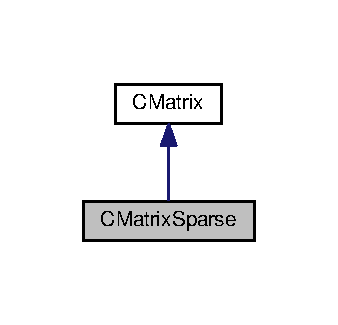
\includegraphics[width=162pt]{classCMatrixSparse__inherit__graph}
\end{center}
\end{figure}


Collaboration diagram for C\+Matrix\+Sparse\+:\nopagebreak
\begin{figure}[H]
\begin{center}
\leavevmode
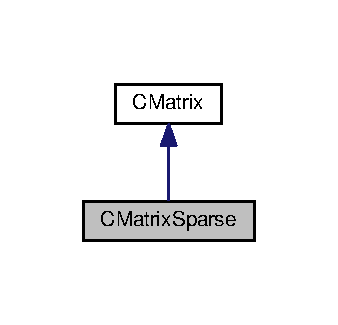
\includegraphics[width=162pt]{classCMatrixSparse__coll__graph}
\end{center}
\end{figure}
\subsection*{Public Member Functions}
\begin{DoxyCompactItemize}
\item 
\hyperlink{classCMatrixSparse_a8b07f6b861304fccebc6229968a0baa0}{C\+Matrix\+Sparse} ()
\item 
\hyperlink{classCMatrixSparse_ab2dc89566f3cdcb626a04fb4c89db926}{C\+Matrix\+Sparse} (const shared\+\_\+ptr$<$ \hyperlink{classCMatrix}{C\+Matrix} $>$ \&other)
\item 
\hyperlink{classCMatrixSparse_a154a1f5510bcedba74fec1eeb6ab4af6}{C\+Matrix\+Sparse} (map$<$ pair$<$ size\+\_\+t, size\+\_\+t $>$, double $>$ matrix, size\+\_\+t num\+Rows, size\+\_\+t num\+Cols)
\item 
\hyperlink{classCMatrixSparse_a2477eb8b3d46d83f067fe3c6fcb37772}{C\+Matrix\+Sparse} (vector$<$ vector$<$ double $>$$>$ matrix)
\item 
\hyperlink{classCMatrix}{C\+Matrix} $\ast$ \hyperlink{classCMatrixSparse_a8074d01357ce15ce0392a95d17fed7ef}{Clone} () const override
\item 
virtual \hyperlink{classCMatrix}{C\+Matrix} $\ast$ \hyperlink{classCMatrixSparse_a1519d4cdef830a6df4d0ec900b4413c7}{Convert} () const override
\item 
virtual \hyperlink{classCMatrixSparse_a40f32c0d13b58937ecbb279b670e9ebc}{$\sim$\+C\+Matrix\+Sparse} () override=default
\item 
virtual double \hyperlink{classCMatrixSparse_a1f071b5ed04bb2fb015f97ce7074702d}{Get\+Num\+At\+Coords} (size\+\_\+t row, size\+\_\+t col) const override
\item 
virtual void \hyperlink{classCMatrixSparse_a675982946fbb61169c625e5eb5d2d2bd}{Set\+Num\+At\+Coords} (size\+\_\+t row, size\+\_\+t col, double value) override
\item 
\hyperlink{classCMatrix}{C\+Matrix} $\ast$ \hyperlink{classCMatrixSparse_a2f545baf72ad2974e1450f8653f9bd06}{Get\+Empty\+Instance} () const override
\item 
void \hyperlink{classCMatrixSparse_a83cd4fce61394f6c2b290bf06d0efd0a}{Resize} (std\+::size\+\_\+t num\+Rows, std\+::size\+\_\+t num\+Cols) override
\item 
virtual void \hyperlink{classCMatrixSparse_acf4a7e41666e6fb29e629c3a62a7fd8f}{Print} () const override
\item 
virtual bool \hyperlink{classCMatrixSparse_a780df7daf904384dadb5f3cd9bd81e40}{Should\+Be\+Sparse} () const 
\item 
virtual void \hyperlink{classCMatrixSparse_a09c9471dbb6d83f6f51f25cc24554293}{Swap\+Rows} (std\+::size\+\_\+t a, std\+::size\+\_\+t b) override
\end{DoxyCompactItemize}
\subsection*{Private Attributes}
\begin{DoxyCompactItemize}
\item 
map$<$ pair$<$ size\+\_\+t, size\+\_\+t $>$, double $>$ \hyperlink{classCMatrixSparse_ae73efeb433e6dee92d020dba745f7fc3}{m\+\_\+\+Matrix}
\end{DoxyCompactItemize}
\subsection*{Additional Inherited Members}


\subsection{Constructor \& Destructor Documentation}
\index{C\+Matrix\+Sparse@{C\+Matrix\+Sparse}!C\+Matrix\+Sparse@{C\+Matrix\+Sparse}}
\index{C\+Matrix\+Sparse@{C\+Matrix\+Sparse}!C\+Matrix\+Sparse@{C\+Matrix\+Sparse}}
\subsubsection[{\texorpdfstring{C\+Matrix\+Sparse()}{CMatrixSparse()}}]{\setlength{\rightskip}{0pt plus 5cm}C\+Matrix\+Sparse\+::\+C\+Matrix\+Sparse (
\begin{DoxyParamCaption}
{}
\end{DoxyParamCaption}
)\hspace{0.3cm}{\ttfamily [inline]}}\hypertarget{classCMatrixSparse_a8b07f6b861304fccebc6229968a0baa0}{}\label{classCMatrixSparse_a8b07f6b861304fccebc6229968a0baa0}
\index{C\+Matrix\+Sparse@{C\+Matrix\+Sparse}!C\+Matrix\+Sparse@{C\+Matrix\+Sparse}}
\index{C\+Matrix\+Sparse@{C\+Matrix\+Sparse}!C\+Matrix\+Sparse@{C\+Matrix\+Sparse}}
\subsubsection[{\texorpdfstring{C\+Matrix\+Sparse(const shared\+\_\+ptr$<$ C\+Matrix $>$ \&other)}{CMatrixSparse(const shared_ptr< CMatrix > &other)}}]{\setlength{\rightskip}{0pt plus 5cm}C\+Matrix\+Sparse\+::\+C\+Matrix\+Sparse (
\begin{DoxyParamCaption}
\item[{const shared\+\_\+ptr$<$ {\bf C\+Matrix} $>$ \&}]{other}
\end{DoxyParamCaption}
)\hspace{0.3cm}{\ttfamily [inline]}}\hypertarget{classCMatrixSparse_ab2dc89566f3cdcb626a04fb4c89db926}{}\label{classCMatrixSparse_ab2dc89566f3cdcb626a04fb4c89db926}
\index{C\+Matrix\+Sparse@{C\+Matrix\+Sparse}!C\+Matrix\+Sparse@{C\+Matrix\+Sparse}}
\index{C\+Matrix\+Sparse@{C\+Matrix\+Sparse}!C\+Matrix\+Sparse@{C\+Matrix\+Sparse}}
\subsubsection[{\texorpdfstring{C\+Matrix\+Sparse(map$<$ pair$<$ size\+\_\+t, size\+\_\+t $>$, double $>$ matrix, size\+\_\+t num\+Rows, size\+\_\+t num\+Cols)}{CMatrixSparse(map< pair< size_t, size_t >, double > matrix, size_t numRows, size_t numCols)}}]{\setlength{\rightskip}{0pt plus 5cm}C\+Matrix\+Sparse\+::\+C\+Matrix\+Sparse (
\begin{DoxyParamCaption}
\item[{map$<$ pair$<$ size\+\_\+t, size\+\_\+t $>$, double $>$}]{matrix, }
\item[{size\+\_\+t}]{num\+Rows, }
\item[{size\+\_\+t}]{num\+Cols}
\end{DoxyParamCaption}
)\hspace{0.3cm}{\ttfamily [inline]}}\hypertarget{classCMatrixSparse_a154a1f5510bcedba74fec1eeb6ab4af6}{}\label{classCMatrixSparse_a154a1f5510bcedba74fec1eeb6ab4af6}
\index{C\+Matrix\+Sparse@{C\+Matrix\+Sparse}!C\+Matrix\+Sparse@{C\+Matrix\+Sparse}}
\index{C\+Matrix\+Sparse@{C\+Matrix\+Sparse}!C\+Matrix\+Sparse@{C\+Matrix\+Sparse}}
\subsubsection[{\texorpdfstring{C\+Matrix\+Sparse(vector$<$ vector$<$ double $>$$>$ matrix)}{CMatrixSparse(vector< vector< double >> matrix)}}]{\setlength{\rightskip}{0pt plus 5cm}C\+Matrix\+Sparse\+::\+C\+Matrix\+Sparse (
\begin{DoxyParamCaption}
\item[{vector$<$ vector$<$ double $>$$>$}]{matrix}
\end{DoxyParamCaption}
)\hspace{0.3cm}{\ttfamily [inline]}}\hypertarget{classCMatrixSparse_a2477eb8b3d46d83f067fe3c6fcb37772}{}\label{classCMatrixSparse_a2477eb8b3d46d83f067fe3c6fcb37772}
\index{C\+Matrix\+Sparse@{C\+Matrix\+Sparse}!````~C\+Matrix\+Sparse@{$\sim$\+C\+Matrix\+Sparse}}
\index{````~C\+Matrix\+Sparse@{$\sim$\+C\+Matrix\+Sparse}!C\+Matrix\+Sparse@{C\+Matrix\+Sparse}}
\subsubsection[{\texorpdfstring{$\sim$\+C\+Matrix\+Sparse() override=default}{~CMatrixSparse() override=default}}]{\setlength{\rightskip}{0pt plus 5cm}virtual C\+Matrix\+Sparse\+::$\sim$\+C\+Matrix\+Sparse (
\begin{DoxyParamCaption}
{}
\end{DoxyParamCaption}
)\hspace{0.3cm}{\ttfamily [override]}, {\ttfamily [virtual]}, {\ttfamily [default]}}\hypertarget{classCMatrixSparse_a40f32c0d13b58937ecbb279b670e9ebc}{}\label{classCMatrixSparse_a40f32c0d13b58937ecbb279b670e9ebc}


\subsection{Member Function Documentation}
\index{C\+Matrix\+Sparse@{C\+Matrix\+Sparse}!Clone@{Clone}}
\index{Clone@{Clone}!C\+Matrix\+Sparse@{C\+Matrix\+Sparse}}
\subsubsection[{\texorpdfstring{Clone() const override}{Clone() const override}}]{\setlength{\rightskip}{0pt plus 5cm}{\bf C\+Matrix}$\ast$ C\+Matrix\+Sparse\+::\+Clone (
\begin{DoxyParamCaption}
{}
\end{DoxyParamCaption}
) const\hspace{0.3cm}{\ttfamily [inline]}, {\ttfamily [override]}, {\ttfamily [virtual]}}\hypertarget{classCMatrixSparse_a8074d01357ce15ce0392a95d17fed7ef}{}\label{classCMatrixSparse_a8074d01357ce15ce0392a95d17fed7ef}


Implements \hyperlink{classCMatrix_a42ac1f2a9e69919974febca17971be60}{C\+Matrix}.

\index{C\+Matrix\+Sparse@{C\+Matrix\+Sparse}!Convert@{Convert}}
\index{Convert@{Convert}!C\+Matrix\+Sparse@{C\+Matrix\+Sparse}}
\subsubsection[{\texorpdfstring{Convert() const override}{Convert() const override}}]{\setlength{\rightskip}{0pt plus 5cm}{\bf C\+Matrix} $\ast$ C\+Matrix\+Sparse\+::\+Convert (
\begin{DoxyParamCaption}
{}
\end{DoxyParamCaption}
) const\hspace{0.3cm}{\ttfamily [override]}, {\ttfamily [virtual]}}\hypertarget{classCMatrixSparse_a1519d4cdef830a6df4d0ec900b4413c7}{}\label{classCMatrixSparse_a1519d4cdef830a6df4d0ec900b4413c7}


Implements \hyperlink{classCMatrix_aca808472e6465738fae14a6ac244cf0b}{C\+Matrix}.

\index{C\+Matrix\+Sparse@{C\+Matrix\+Sparse}!Get\+Empty\+Instance@{Get\+Empty\+Instance}}
\index{Get\+Empty\+Instance@{Get\+Empty\+Instance}!C\+Matrix\+Sparse@{C\+Matrix\+Sparse}}
\subsubsection[{\texorpdfstring{Get\+Empty\+Instance() const override}{GetEmptyInstance() const override}}]{\setlength{\rightskip}{0pt plus 5cm}{\bf C\+Matrix}$\ast$ C\+Matrix\+Sparse\+::\+Get\+Empty\+Instance (
\begin{DoxyParamCaption}
{}
\end{DoxyParamCaption}
) const\hspace{0.3cm}{\ttfamily [inline]}, {\ttfamily [override]}, {\ttfamily [virtual]}}\hypertarget{classCMatrixSparse_a2f545baf72ad2974e1450f8653f9bd06}{}\label{classCMatrixSparse_a2f545baf72ad2974e1450f8653f9bd06}


Implements \hyperlink{classCMatrix_a7495208c2bd786fe46b130f6090e7eb5}{C\+Matrix}.

\index{C\+Matrix\+Sparse@{C\+Matrix\+Sparse}!Get\+Num\+At\+Coords@{Get\+Num\+At\+Coords}}
\index{Get\+Num\+At\+Coords@{Get\+Num\+At\+Coords}!C\+Matrix\+Sparse@{C\+Matrix\+Sparse}}
\subsubsection[{\texorpdfstring{Get\+Num\+At\+Coords(size\+\_\+t row, size\+\_\+t col) const override}{GetNumAtCoords(size_t row, size_t col) const override}}]{\setlength{\rightskip}{0pt plus 5cm}double C\+Matrix\+Sparse\+::\+Get\+Num\+At\+Coords (
\begin{DoxyParamCaption}
\item[{size\+\_\+t}]{row, }
\item[{size\+\_\+t}]{col}
\end{DoxyParamCaption}
) const\hspace{0.3cm}{\ttfamily [override]}, {\ttfamily [virtual]}}\hypertarget{classCMatrixSparse_a1f071b5ed04bb2fb015f97ce7074702d}{}\label{classCMatrixSparse_a1f071b5ed04bb2fb015f97ce7074702d}


Implements \hyperlink{classCMatrix_afa0213e0a6c5823e6b6e786891cc5f2d}{C\+Matrix}.

\index{C\+Matrix\+Sparse@{C\+Matrix\+Sparse}!Print@{Print}}
\index{Print@{Print}!C\+Matrix\+Sparse@{C\+Matrix\+Sparse}}
\subsubsection[{\texorpdfstring{Print() const override}{Print() const override}}]{\setlength{\rightskip}{0pt plus 5cm}void C\+Matrix\+Sparse\+::\+Print (
\begin{DoxyParamCaption}
{}
\end{DoxyParamCaption}
) const\hspace{0.3cm}{\ttfamily [override]}, {\ttfamily [virtual]}}\hypertarget{classCMatrixSparse_acf4a7e41666e6fb29e629c3a62a7fd8f}{}\label{classCMatrixSparse_acf4a7e41666e6fb29e629c3a62a7fd8f}


Implements \hyperlink{classCMatrix_a424a048d20918f0f041f4a8645823ae7}{C\+Matrix}.

\index{C\+Matrix\+Sparse@{C\+Matrix\+Sparse}!Resize@{Resize}}
\index{Resize@{Resize}!C\+Matrix\+Sparse@{C\+Matrix\+Sparse}}
\subsubsection[{\texorpdfstring{Resize(std\+::size\+\_\+t num\+Rows, std\+::size\+\_\+t num\+Cols) override}{Resize(std::size_t numRows, std::size_t numCols) override}}]{\setlength{\rightskip}{0pt plus 5cm}void C\+Matrix\+Sparse\+::\+Resize (
\begin{DoxyParamCaption}
\item[{std\+::size\+\_\+t}]{num\+Rows, }
\item[{std\+::size\+\_\+t}]{num\+Cols}
\end{DoxyParamCaption}
)\hspace{0.3cm}{\ttfamily [inline]}, {\ttfamily [override]}, {\ttfamily [virtual]}}\hypertarget{classCMatrixSparse_a83cd4fce61394f6c2b290bf06d0efd0a}{}\label{classCMatrixSparse_a83cd4fce61394f6c2b290bf06d0efd0a}


Implements \hyperlink{classCMatrix_adb83eafeeea2025f9c84d172f1bb0f1e}{C\+Matrix}.

\index{C\+Matrix\+Sparse@{C\+Matrix\+Sparse}!Set\+Num\+At\+Coords@{Set\+Num\+At\+Coords}}
\index{Set\+Num\+At\+Coords@{Set\+Num\+At\+Coords}!C\+Matrix\+Sparse@{C\+Matrix\+Sparse}}
\subsubsection[{\texorpdfstring{Set\+Num\+At\+Coords(size\+\_\+t row, size\+\_\+t col, double value) override}{SetNumAtCoords(size_t row, size_t col, double value) override}}]{\setlength{\rightskip}{0pt plus 5cm}virtual void C\+Matrix\+Sparse\+::\+Set\+Num\+At\+Coords (
\begin{DoxyParamCaption}
\item[{size\+\_\+t}]{row, }
\item[{size\+\_\+t}]{col, }
\item[{double}]{value}
\end{DoxyParamCaption}
)\hspace{0.3cm}{\ttfamily [inline]}, {\ttfamily [override]}, {\ttfamily [virtual]}}\hypertarget{classCMatrixSparse_a675982946fbb61169c625e5eb5d2d2bd}{}\label{classCMatrixSparse_a675982946fbb61169c625e5eb5d2d2bd}


Implements \hyperlink{classCMatrix_afeba0f7cfcc2623bde41cf6111b0ef6a}{C\+Matrix}.

\index{C\+Matrix\+Sparse@{C\+Matrix\+Sparse}!Should\+Be\+Sparse@{Should\+Be\+Sparse}}
\index{Should\+Be\+Sparse@{Should\+Be\+Sparse}!C\+Matrix\+Sparse@{C\+Matrix\+Sparse}}
\subsubsection[{\texorpdfstring{Should\+Be\+Sparse() const }{ShouldBeSparse() const }}]{\setlength{\rightskip}{0pt plus 5cm}virtual bool C\+Matrix\+Sparse\+::\+Should\+Be\+Sparse (
\begin{DoxyParamCaption}
{}
\end{DoxyParamCaption}
) const\hspace{0.3cm}{\ttfamily [inline]}, {\ttfamily [virtual]}}\hypertarget{classCMatrixSparse_a780df7daf904384dadb5f3cd9bd81e40}{}\label{classCMatrixSparse_a780df7daf904384dadb5f3cd9bd81e40}


Implements \hyperlink{classCMatrix_a668eaab1f5d9b498e721464124f158c4}{C\+Matrix}.

\index{C\+Matrix\+Sparse@{C\+Matrix\+Sparse}!Swap\+Rows@{Swap\+Rows}}
\index{Swap\+Rows@{Swap\+Rows}!C\+Matrix\+Sparse@{C\+Matrix\+Sparse}}
\subsubsection[{\texorpdfstring{Swap\+Rows(std\+::size\+\_\+t a, std\+::size\+\_\+t b) override}{SwapRows(std::size_t a, std::size_t b) override}}]{\setlength{\rightskip}{0pt plus 5cm}virtual void C\+Matrix\+Sparse\+::\+Swap\+Rows (
\begin{DoxyParamCaption}
\item[{std\+::size\+\_\+t}]{a, }
\item[{std\+::size\+\_\+t}]{b}
\end{DoxyParamCaption}
)\hspace{0.3cm}{\ttfamily [inline]}, {\ttfamily [override]}, {\ttfamily [virtual]}}\hypertarget{classCMatrixSparse_a09c9471dbb6d83f6f51f25cc24554293}{}\label{classCMatrixSparse_a09c9471dbb6d83f6f51f25cc24554293}


Implements \hyperlink{classCMatrix_aa9f96d82fa2e564f89f35a1781a12d69}{C\+Matrix}.



\subsection{Member Data Documentation}
\index{C\+Matrix\+Sparse@{C\+Matrix\+Sparse}!m\+\_\+\+Matrix@{m\+\_\+\+Matrix}}
\index{m\+\_\+\+Matrix@{m\+\_\+\+Matrix}!C\+Matrix\+Sparse@{C\+Matrix\+Sparse}}
\subsubsection[{\texorpdfstring{m\+\_\+\+Matrix}{m_Matrix}}]{\setlength{\rightskip}{0pt plus 5cm}map$<$pair$<$size\+\_\+t, size\+\_\+t$>$, double$>$ C\+Matrix\+Sparse\+::m\+\_\+\+Matrix\hspace{0.3cm}{\ttfamily [private]}}\hypertarget{classCMatrixSparse_ae73efeb433e6dee92d020dba745f7fc3}{}\label{classCMatrixSparse_ae73efeb433e6dee92d020dba745f7fc3}


The documentation for this class was generated from the following files\+:\begin{DoxyCompactItemize}
\item 
src/\hyperlink{CMatrixSparse_8h}{C\+Matrix\+Sparse.\+h}\item 
src/\hyperlink{CMatrixSparse_8cpp}{C\+Matrix\+Sparse.\+cpp}\end{DoxyCompactItemize}

\hypertarget{classCMatrixStandard}{}\section{C\+Matrix\+Standard Class Reference}
\label{classCMatrixStandard}\index{C\+Matrix\+Standard@{C\+Matrix\+Standard}}


{\ttfamily \#include $<$C\+Matrix\+Standard.\+h$>$}



Inheritance diagram for C\+Matrix\+Standard\+:\nopagebreak
\begin{figure}[H]
\begin{center}
\leavevmode
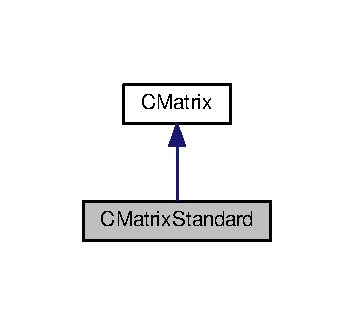
\includegraphics[width=170pt]{classCMatrixStandard__inherit__graph}
\end{center}
\end{figure}


Collaboration diagram for C\+Matrix\+Standard\+:\nopagebreak
\begin{figure}[H]
\begin{center}
\leavevmode
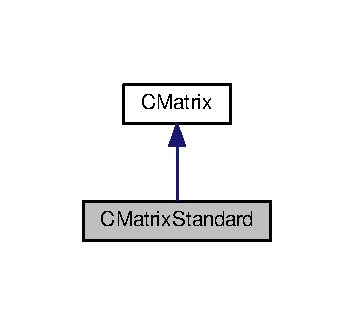
\includegraphics[width=170pt]{classCMatrixStandard__coll__graph}
\end{center}
\end{figure}
\subsection*{Public Member Functions}
\begin{DoxyCompactItemize}
\item 
\hyperlink{classCMatrixStandard_ad862ccde0cbe3a1f72e724091040475d}{C\+Matrix\+Standard} ()
\item 
\hyperlink{classCMatrixStandard_a5ae792cb1f82cfd0f8710f22e6c03588}{C\+Matrix\+Standard} (vector$<$ vector$<$ double $>$$>$ matrix)
\item 
\hyperlink{classCMatrixStandard_ae2f8784f0d63aab266bbd144c5cc10c6}{C\+Matrix\+Standard} (map$<$ pair$<$ size\+\_\+t, size\+\_\+t $>$, double $>$ matrix, size\+\_\+t num\+Rows, size\+\_\+t num\+Cols)
\item 
virtual void \hyperlink{classCMatrixStandard_a8c8a6ce02302a423928b725e41c7730a}{Swap\+Rows} (std\+::size\+\_\+t a, std\+::size\+\_\+t b) override
\item 
\hyperlink{classCMatrix}{C\+Matrix} $\ast$ \hyperlink{classCMatrixStandard_a30885c9a67bfe07b8379f7dd7a782ce4}{Clone} () const override
\item 
virtual \hyperlink{classCMatrix}{C\+Matrix} $\ast$ \hyperlink{classCMatrixStandard_a73f39b1ac5602dbd233df469ba8f0c3b}{Convert} () const override
\item 
virtual \hyperlink{classCMatrixStandard_af1c8dfb0c0bdc2933fe19dc7deef0a80}{$\sim$\+C\+Matrix\+Standard} () override=default
\item 
virtual void \hyperlink{classCMatrixStandard_a0ace6054f9ec1fb2b26e0683034e48bd}{Print} () const override
\item 
virtual double \hyperlink{classCMatrixStandard_a277c77a453dccdac55de180bb63a8a7f}{Get\+Num\+At\+Coords} (size\+\_\+t row, size\+\_\+t col) const override
\item 
virtual void \hyperlink{classCMatrixStandard_a7fe5561630fbc65f7aeac5bd54499c13}{Set\+Num\+At\+Coords} (size\+\_\+t row, size\+\_\+t col, double value) override
\item 
\hyperlink{classCMatrix}{C\+Matrix} $\ast$ \hyperlink{classCMatrixStandard_a17e51335d1d9e731441a8205536697f7}{Get\+Empty\+Instance} () const override
\item 
void \hyperlink{classCMatrixStandard_ad135e13127c58f91c325a131d1dc8a74}{Resize} (std\+::size\+\_\+t num\+Rows, std\+::size\+\_\+t num\+Cols) override
\item 
virtual bool \hyperlink{classCMatrixStandard_a603dcb22f4cdf94438d4e59fe44870e4}{Should\+Be\+Sparse} () const override
\end{DoxyCompactItemize}
\subsection*{Private Attributes}
\begin{DoxyCompactItemize}
\item 
vector$<$ vector$<$ double $>$ $>$ \hyperlink{classCMatrixStandard_a4b0bafe59e3358e0d3fdbcc42b584dec}{m\+\_\+\+Matrix}
\end{DoxyCompactItemize}
\subsection*{Additional Inherited Members}


\subsection{Constructor \& Destructor Documentation}
\index{C\+Matrix\+Standard@{C\+Matrix\+Standard}!C\+Matrix\+Standard@{C\+Matrix\+Standard}}
\index{C\+Matrix\+Standard@{C\+Matrix\+Standard}!C\+Matrix\+Standard@{C\+Matrix\+Standard}}
\subsubsection[{\texorpdfstring{C\+Matrix\+Standard()}{CMatrixStandard()}}]{\setlength{\rightskip}{0pt plus 5cm}C\+Matrix\+Standard\+::\+C\+Matrix\+Standard (
\begin{DoxyParamCaption}
{}
\end{DoxyParamCaption}
)\hspace{0.3cm}{\ttfamily [inline]}}\hypertarget{classCMatrixStandard_ad862ccde0cbe3a1f72e724091040475d}{}\label{classCMatrixStandard_ad862ccde0cbe3a1f72e724091040475d}
\index{C\+Matrix\+Standard@{C\+Matrix\+Standard}!C\+Matrix\+Standard@{C\+Matrix\+Standard}}
\index{C\+Matrix\+Standard@{C\+Matrix\+Standard}!C\+Matrix\+Standard@{C\+Matrix\+Standard}}
\subsubsection[{\texorpdfstring{C\+Matrix\+Standard(vector$<$ vector$<$ double $>$$>$ matrix)}{CMatrixStandard(vector< vector< double >> matrix)}}]{\setlength{\rightskip}{0pt plus 5cm}C\+Matrix\+Standard\+::\+C\+Matrix\+Standard (
\begin{DoxyParamCaption}
\item[{vector$<$ vector$<$ double $>$$>$}]{matrix}
\end{DoxyParamCaption}
)\hspace{0.3cm}{\ttfamily [inline]}}\hypertarget{classCMatrixStandard_a5ae792cb1f82cfd0f8710f22e6c03588}{}\label{classCMatrixStandard_a5ae792cb1f82cfd0f8710f22e6c03588}
\index{C\+Matrix\+Standard@{C\+Matrix\+Standard}!C\+Matrix\+Standard@{C\+Matrix\+Standard}}
\index{C\+Matrix\+Standard@{C\+Matrix\+Standard}!C\+Matrix\+Standard@{C\+Matrix\+Standard}}
\subsubsection[{\texorpdfstring{C\+Matrix\+Standard(map$<$ pair$<$ size\+\_\+t, size\+\_\+t $>$, double $>$ matrix, size\+\_\+t num\+Rows, size\+\_\+t num\+Cols)}{CMatrixStandard(map< pair< size_t, size_t >, double > matrix, size_t numRows, size_t numCols)}}]{\setlength{\rightskip}{0pt plus 5cm}C\+Matrix\+Standard\+::\+C\+Matrix\+Standard (
\begin{DoxyParamCaption}
\item[{map$<$ pair$<$ size\+\_\+t, size\+\_\+t $>$, double $>$}]{matrix, }
\item[{size\+\_\+t}]{num\+Rows, }
\item[{size\+\_\+t}]{num\+Cols}
\end{DoxyParamCaption}
)\hspace{0.3cm}{\ttfamily [inline]}}\hypertarget{classCMatrixStandard_ae2f8784f0d63aab266bbd144c5cc10c6}{}\label{classCMatrixStandard_ae2f8784f0d63aab266bbd144c5cc10c6}
\index{C\+Matrix\+Standard@{C\+Matrix\+Standard}!````~C\+Matrix\+Standard@{$\sim$\+C\+Matrix\+Standard}}
\index{````~C\+Matrix\+Standard@{$\sim$\+C\+Matrix\+Standard}!C\+Matrix\+Standard@{C\+Matrix\+Standard}}
\subsubsection[{\texorpdfstring{$\sim$\+C\+Matrix\+Standard() override=default}{~CMatrixStandard() override=default}}]{\setlength{\rightskip}{0pt plus 5cm}virtual C\+Matrix\+Standard\+::$\sim$\+C\+Matrix\+Standard (
\begin{DoxyParamCaption}
{}
\end{DoxyParamCaption}
)\hspace{0.3cm}{\ttfamily [override]}, {\ttfamily [virtual]}, {\ttfamily [default]}}\hypertarget{classCMatrixStandard_af1c8dfb0c0bdc2933fe19dc7deef0a80}{}\label{classCMatrixStandard_af1c8dfb0c0bdc2933fe19dc7deef0a80}


\subsection{Member Function Documentation}
\index{C\+Matrix\+Standard@{C\+Matrix\+Standard}!Clone@{Clone}}
\index{Clone@{Clone}!C\+Matrix\+Standard@{C\+Matrix\+Standard}}
\subsubsection[{\texorpdfstring{Clone() const override}{Clone() const override}}]{\setlength{\rightskip}{0pt plus 5cm}{\bf C\+Matrix}$\ast$ C\+Matrix\+Standard\+::\+Clone (
\begin{DoxyParamCaption}
{}
\end{DoxyParamCaption}
) const\hspace{0.3cm}{\ttfamily [inline]}, {\ttfamily [override]}, {\ttfamily [virtual]}}\hypertarget{classCMatrixStandard_a30885c9a67bfe07b8379f7dd7a782ce4}{}\label{classCMatrixStandard_a30885c9a67bfe07b8379f7dd7a782ce4}


Implements \hyperlink{classCMatrix_a42ac1f2a9e69919974febca17971be60}{C\+Matrix}.

\index{C\+Matrix\+Standard@{C\+Matrix\+Standard}!Convert@{Convert}}
\index{Convert@{Convert}!C\+Matrix\+Standard@{C\+Matrix\+Standard}}
\subsubsection[{\texorpdfstring{Convert() const override}{Convert() const override}}]{\setlength{\rightskip}{0pt plus 5cm}{\bf C\+Matrix} $\ast$ C\+Matrix\+Standard\+::\+Convert (
\begin{DoxyParamCaption}
{}
\end{DoxyParamCaption}
) const\hspace{0.3cm}{\ttfamily [override]}, {\ttfamily [virtual]}}\hypertarget{classCMatrixStandard_a73f39b1ac5602dbd233df469ba8f0c3b}{}\label{classCMatrixStandard_a73f39b1ac5602dbd233df469ba8f0c3b}


Implements \hyperlink{classCMatrix_aca808472e6465738fae14a6ac244cf0b}{C\+Matrix}.

\index{C\+Matrix\+Standard@{C\+Matrix\+Standard}!Get\+Empty\+Instance@{Get\+Empty\+Instance}}
\index{Get\+Empty\+Instance@{Get\+Empty\+Instance}!C\+Matrix\+Standard@{C\+Matrix\+Standard}}
\subsubsection[{\texorpdfstring{Get\+Empty\+Instance() const override}{GetEmptyInstance() const override}}]{\setlength{\rightskip}{0pt plus 5cm}{\bf C\+Matrix}$\ast$ C\+Matrix\+Standard\+::\+Get\+Empty\+Instance (
\begin{DoxyParamCaption}
{}
\end{DoxyParamCaption}
) const\hspace{0.3cm}{\ttfamily [inline]}, {\ttfamily [override]}, {\ttfamily [virtual]}}\hypertarget{classCMatrixStandard_a17e51335d1d9e731441a8205536697f7}{}\label{classCMatrixStandard_a17e51335d1d9e731441a8205536697f7}


Implements \hyperlink{classCMatrix_a7495208c2bd786fe46b130f6090e7eb5}{C\+Matrix}.

\index{C\+Matrix\+Standard@{C\+Matrix\+Standard}!Get\+Num\+At\+Coords@{Get\+Num\+At\+Coords}}
\index{Get\+Num\+At\+Coords@{Get\+Num\+At\+Coords}!C\+Matrix\+Standard@{C\+Matrix\+Standard}}
\subsubsection[{\texorpdfstring{Get\+Num\+At\+Coords(size\+\_\+t row, size\+\_\+t col) const override}{GetNumAtCoords(size_t row, size_t col) const override}}]{\setlength{\rightskip}{0pt plus 5cm}virtual double C\+Matrix\+Standard\+::\+Get\+Num\+At\+Coords (
\begin{DoxyParamCaption}
\item[{size\+\_\+t}]{row, }
\item[{size\+\_\+t}]{col}
\end{DoxyParamCaption}
) const\hspace{0.3cm}{\ttfamily [inline]}, {\ttfamily [override]}, {\ttfamily [virtual]}}\hypertarget{classCMatrixStandard_a277c77a453dccdac55de180bb63a8a7f}{}\label{classCMatrixStandard_a277c77a453dccdac55de180bb63a8a7f}


Implements \hyperlink{classCMatrix_afa0213e0a6c5823e6b6e786891cc5f2d}{C\+Matrix}.

\index{C\+Matrix\+Standard@{C\+Matrix\+Standard}!Print@{Print}}
\index{Print@{Print}!C\+Matrix\+Standard@{C\+Matrix\+Standard}}
\subsubsection[{\texorpdfstring{Print() const override}{Print() const override}}]{\setlength{\rightskip}{0pt plus 5cm}void C\+Matrix\+Standard\+::\+Print (
\begin{DoxyParamCaption}
{}
\end{DoxyParamCaption}
) const\hspace{0.3cm}{\ttfamily [override]}, {\ttfamily [virtual]}}\hypertarget{classCMatrixStandard_a0ace6054f9ec1fb2b26e0683034e48bd}{}\label{classCMatrixStandard_a0ace6054f9ec1fb2b26e0683034e48bd}


Implements \hyperlink{classCMatrix_a424a048d20918f0f041f4a8645823ae7}{C\+Matrix}.

\index{C\+Matrix\+Standard@{C\+Matrix\+Standard}!Resize@{Resize}}
\index{Resize@{Resize}!C\+Matrix\+Standard@{C\+Matrix\+Standard}}
\subsubsection[{\texorpdfstring{Resize(std\+::size\+\_\+t num\+Rows, std\+::size\+\_\+t num\+Cols) override}{Resize(std::size_t numRows, std::size_t numCols) override}}]{\setlength{\rightskip}{0pt plus 5cm}void C\+Matrix\+Standard\+::\+Resize (
\begin{DoxyParamCaption}
\item[{std\+::size\+\_\+t}]{num\+Rows, }
\item[{std\+::size\+\_\+t}]{num\+Cols}
\end{DoxyParamCaption}
)\hspace{0.3cm}{\ttfamily [inline]}, {\ttfamily [override]}, {\ttfamily [virtual]}}\hypertarget{classCMatrixStandard_ad135e13127c58f91c325a131d1dc8a74}{}\label{classCMatrixStandard_ad135e13127c58f91c325a131d1dc8a74}


Implements \hyperlink{classCMatrix_adb83eafeeea2025f9c84d172f1bb0f1e}{C\+Matrix}.

\index{C\+Matrix\+Standard@{C\+Matrix\+Standard}!Set\+Num\+At\+Coords@{Set\+Num\+At\+Coords}}
\index{Set\+Num\+At\+Coords@{Set\+Num\+At\+Coords}!C\+Matrix\+Standard@{C\+Matrix\+Standard}}
\subsubsection[{\texorpdfstring{Set\+Num\+At\+Coords(size\+\_\+t row, size\+\_\+t col, double value) override}{SetNumAtCoords(size_t row, size_t col, double value) override}}]{\setlength{\rightskip}{0pt plus 5cm}virtual void C\+Matrix\+Standard\+::\+Set\+Num\+At\+Coords (
\begin{DoxyParamCaption}
\item[{size\+\_\+t}]{row, }
\item[{size\+\_\+t}]{col, }
\item[{double}]{value}
\end{DoxyParamCaption}
)\hspace{0.3cm}{\ttfamily [inline]}, {\ttfamily [override]}, {\ttfamily [virtual]}}\hypertarget{classCMatrixStandard_a7fe5561630fbc65f7aeac5bd54499c13}{}\label{classCMatrixStandard_a7fe5561630fbc65f7aeac5bd54499c13}


Implements \hyperlink{classCMatrix_afeba0f7cfcc2623bde41cf6111b0ef6a}{C\+Matrix}.

\index{C\+Matrix\+Standard@{C\+Matrix\+Standard}!Should\+Be\+Sparse@{Should\+Be\+Sparse}}
\index{Should\+Be\+Sparse@{Should\+Be\+Sparse}!C\+Matrix\+Standard@{C\+Matrix\+Standard}}
\subsubsection[{\texorpdfstring{Should\+Be\+Sparse() const override}{ShouldBeSparse() const override}}]{\setlength{\rightskip}{0pt plus 5cm}virtual bool C\+Matrix\+Standard\+::\+Should\+Be\+Sparse (
\begin{DoxyParamCaption}
{}
\end{DoxyParamCaption}
) const\hspace{0.3cm}{\ttfamily [inline]}, {\ttfamily [override]}, {\ttfamily [virtual]}}\hypertarget{classCMatrixStandard_a603dcb22f4cdf94438d4e59fe44870e4}{}\label{classCMatrixStandard_a603dcb22f4cdf94438d4e59fe44870e4}


Implements \hyperlink{classCMatrix_a668eaab1f5d9b498e721464124f158c4}{C\+Matrix}.

\index{C\+Matrix\+Standard@{C\+Matrix\+Standard}!Swap\+Rows@{Swap\+Rows}}
\index{Swap\+Rows@{Swap\+Rows}!C\+Matrix\+Standard@{C\+Matrix\+Standard}}
\subsubsection[{\texorpdfstring{Swap\+Rows(std\+::size\+\_\+t a, std\+::size\+\_\+t b) override}{SwapRows(std::size_t a, std::size_t b) override}}]{\setlength{\rightskip}{0pt plus 5cm}virtual void C\+Matrix\+Standard\+::\+Swap\+Rows (
\begin{DoxyParamCaption}
\item[{std\+::size\+\_\+t}]{a, }
\item[{std\+::size\+\_\+t}]{b}
\end{DoxyParamCaption}
)\hspace{0.3cm}{\ttfamily [inline]}, {\ttfamily [override]}, {\ttfamily [virtual]}}\hypertarget{classCMatrixStandard_a8c8a6ce02302a423928b725e41c7730a}{}\label{classCMatrixStandard_a8c8a6ce02302a423928b725e41c7730a}


Implements \hyperlink{classCMatrix_aa9f96d82fa2e564f89f35a1781a12d69}{C\+Matrix}.



\subsection{Member Data Documentation}
\index{C\+Matrix\+Standard@{C\+Matrix\+Standard}!m\+\_\+\+Matrix@{m\+\_\+\+Matrix}}
\index{m\+\_\+\+Matrix@{m\+\_\+\+Matrix}!C\+Matrix\+Standard@{C\+Matrix\+Standard}}
\subsubsection[{\texorpdfstring{m\+\_\+\+Matrix}{m_Matrix}}]{\setlength{\rightskip}{0pt plus 5cm}vector$<$vector$<$double$>$ $>$ C\+Matrix\+Standard\+::m\+\_\+\+Matrix\hspace{0.3cm}{\ttfamily [private]}}\hypertarget{classCMatrixStandard_a4b0bafe59e3358e0d3fdbcc42b584dec}{}\label{classCMatrixStandard_a4b0bafe59e3358e0d3fdbcc42b584dec}


The documentation for this class was generated from the following files\+:\begin{DoxyCompactItemize}
\item 
src/\hyperlink{CMatrixStandard_8h}{C\+Matrix\+Standard.\+h}\item 
src/\hyperlink{CMatrixStandard_8cpp}{C\+Matrix\+Standard.\+cpp}\end{DoxyCompactItemize}

\hypertarget{classCMemory}{}\section{C\+Memory Class Reference}
\label{classCMemory}\index{C\+Memory@{C\+Memory}}


{\ttfamily \#include $<$C\+Memory.\+h$>$}

\subsection*{Public Member Functions}
\begin{DoxyCompactItemize}
\item 
\hyperlink{classCMemory_a22d9515f529cb75e01afceeebde200e6}{C\+Memory} ()=default
\item 
\hyperlink{classCMemory_a32ed4aae31101111d8fd9fb1f0aa23b2}{$\sim$\+C\+Memory} ()=default
\item 
bool \hyperlink{classCMemory_a6bef7b5dcb74f3ccc1aac02457928a4d}{Exists\+Variable} (string name) const 
\end{DoxyCompactItemize}
\subsection*{Public Attributes}
\begin{DoxyCompactItemize}
\item 
map$<$ string, shared\+\_\+ptr$<$ class \hyperlink{classCMatrix}{C\+Matrix} $>$ $>$ \hyperlink{classCMemory_a541cc8bf0e073f047e43e9d512aefbe7}{m\+\_\+\+Variables}
\end{DoxyCompactItemize}


\subsection{Constructor \& Destructor Documentation}
\index{C\+Memory@{C\+Memory}!C\+Memory@{C\+Memory}}
\index{C\+Memory@{C\+Memory}!C\+Memory@{C\+Memory}}
\subsubsection[{\texorpdfstring{C\+Memory()=default}{CMemory()=default}}]{\setlength{\rightskip}{0pt plus 5cm}C\+Memory\+::\+C\+Memory (
\begin{DoxyParamCaption}
{}
\end{DoxyParamCaption}
)\hspace{0.3cm}{\ttfamily [default]}}\hypertarget{classCMemory_a22d9515f529cb75e01afceeebde200e6}{}\label{classCMemory_a22d9515f529cb75e01afceeebde200e6}
\index{C\+Memory@{C\+Memory}!````~C\+Memory@{$\sim$\+C\+Memory}}
\index{````~C\+Memory@{$\sim$\+C\+Memory}!C\+Memory@{C\+Memory}}
\subsubsection[{\texorpdfstring{$\sim$\+C\+Memory()=default}{~CMemory()=default}}]{\setlength{\rightskip}{0pt plus 5cm}C\+Memory\+::$\sim$\+C\+Memory (
\begin{DoxyParamCaption}
{}
\end{DoxyParamCaption}
)\hspace{0.3cm}{\ttfamily [default]}}\hypertarget{classCMemory_a32ed4aae31101111d8fd9fb1f0aa23b2}{}\label{classCMemory_a32ed4aae31101111d8fd9fb1f0aa23b2}


\subsection{Member Function Documentation}
\index{C\+Memory@{C\+Memory}!Exists\+Variable@{Exists\+Variable}}
\index{Exists\+Variable@{Exists\+Variable}!C\+Memory@{C\+Memory}}
\subsubsection[{\texorpdfstring{Exists\+Variable(string name) const }{ExistsVariable(string name) const }}]{\setlength{\rightskip}{0pt plus 5cm}bool C\+Memory\+::\+Exists\+Variable (
\begin{DoxyParamCaption}
\item[{string}]{name}
\end{DoxyParamCaption}
) const\hspace{0.3cm}{\ttfamily [inline]}}\hypertarget{classCMemory_a6bef7b5dcb74f3ccc1aac02457928a4d}{}\label{classCMemory_a6bef7b5dcb74f3ccc1aac02457928a4d}


\subsection{Member Data Documentation}
\index{C\+Memory@{C\+Memory}!m\+\_\+\+Variables@{m\+\_\+\+Variables}}
\index{m\+\_\+\+Variables@{m\+\_\+\+Variables}!C\+Memory@{C\+Memory}}
\subsubsection[{\texorpdfstring{m\+\_\+\+Variables}{m_Variables}}]{\setlength{\rightskip}{0pt plus 5cm}map$<$string, shared\+\_\+ptr$<$class {\bf C\+Matrix}$>$ $>$ C\+Memory\+::m\+\_\+\+Variables}\hypertarget{classCMemory_a541cc8bf0e073f047e43e9d512aefbe7}{}\label{classCMemory_a541cc8bf0e073f047e43e9d512aefbe7}


The documentation for this class was generated from the following file\+:\begin{DoxyCompactItemize}
\item 
src/\hyperlink{CMemory_8h}{C\+Memory.\+h}\end{DoxyCompactItemize}

\hypertarget{classCMergeNextToOperator}{}\section{C\+Merge\+Next\+To\+Operator Class Reference}
\label{classCMergeNextToOperator}\index{C\+Merge\+Next\+To\+Operator@{C\+Merge\+Next\+To\+Operator}}


{\ttfamily \#include $<$C\+Merge\+Next\+To\+Operator.\+h$>$}



Inheritance diagram for C\+Merge\+Next\+To\+Operator\+:\nopagebreak
\begin{figure}[H]
\begin{center}
\leavevmode
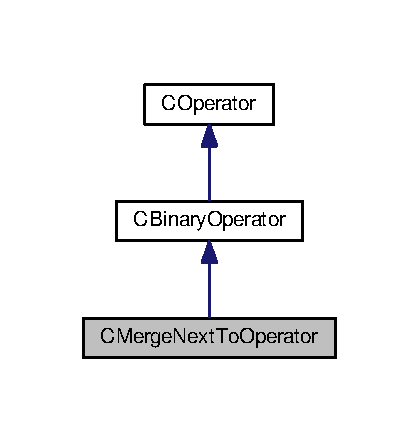
\includegraphics[width=201pt]{classCMergeNextToOperator__inherit__graph}
\end{center}
\end{figure}


Collaboration diagram for C\+Merge\+Next\+To\+Operator\+:\nopagebreak
\begin{figure}[H]
\begin{center}
\leavevmode
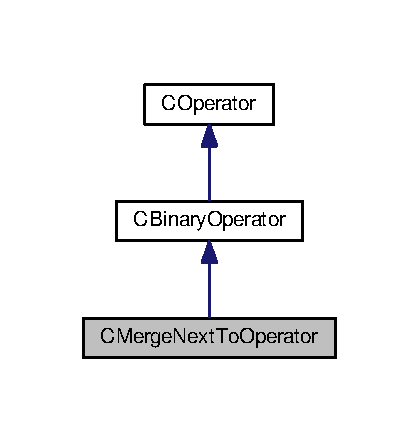
\includegraphics[width=201pt]{classCMergeNextToOperator__coll__graph}
\end{center}
\end{figure}
\subsection*{Public Member Functions}
\begin{DoxyCompactItemize}
\item 
\hyperlink{classCMergeNextToOperator_a83123623e3c2094dad8eda046a171da9}{C\+Merge\+Next\+To\+Operator} (shared\+\_\+ptr$<$ \hyperlink{classCMatrix}{C\+Matrix} $>$ \&left, shared\+\_\+ptr$<$ \hyperlink{classCMatrix}{C\+Matrix} $>$ \&right)
\item 
\hyperlink{classCMatrix}{C\+Matrix} $\ast$ \hyperlink{classCMergeNextToOperator_ab914c0ae204819b6f5e9d9857acd1854}{Evaluate} (\hyperlink{classCMemory}{C\+Memory} \&memory) override
\end{DoxyCompactItemize}
\subsection*{Additional Inherited Members}


\subsection{Constructor \& Destructor Documentation}
\index{C\+Merge\+Next\+To\+Operator@{C\+Merge\+Next\+To\+Operator}!C\+Merge\+Next\+To\+Operator@{C\+Merge\+Next\+To\+Operator}}
\index{C\+Merge\+Next\+To\+Operator@{C\+Merge\+Next\+To\+Operator}!C\+Merge\+Next\+To\+Operator@{C\+Merge\+Next\+To\+Operator}}
\subsubsection[{\texorpdfstring{C\+Merge\+Next\+To\+Operator(shared\+\_\+ptr$<$ C\+Matrix $>$ \&left, shared\+\_\+ptr$<$ C\+Matrix $>$ \&right)}{CMergeNextToOperator(shared_ptr< CMatrix > &left, shared_ptr< CMatrix > &right)}}]{\setlength{\rightskip}{0pt plus 5cm}C\+Merge\+Next\+To\+Operator\+::\+C\+Merge\+Next\+To\+Operator (
\begin{DoxyParamCaption}
\item[{shared\+\_\+ptr$<$ {\bf C\+Matrix} $>$ \&}]{left, }
\item[{shared\+\_\+ptr$<$ {\bf C\+Matrix} $>$ \&}]{right}
\end{DoxyParamCaption}
)\hspace{0.3cm}{\ttfamily [inline]}}\hypertarget{classCMergeNextToOperator_a83123623e3c2094dad8eda046a171da9}{}\label{classCMergeNextToOperator_a83123623e3c2094dad8eda046a171da9}


\subsection{Member Function Documentation}
\index{C\+Merge\+Next\+To\+Operator@{C\+Merge\+Next\+To\+Operator}!Evaluate@{Evaluate}}
\index{Evaluate@{Evaluate}!C\+Merge\+Next\+To\+Operator@{C\+Merge\+Next\+To\+Operator}}
\subsubsection[{\texorpdfstring{Evaluate(\+C\+Memory \&memory) override}{Evaluate(CMemory &memory) override}}]{\setlength{\rightskip}{0pt plus 5cm}{\bf C\+Matrix}$\ast$ C\+Merge\+Next\+To\+Operator\+::\+Evaluate (
\begin{DoxyParamCaption}
\item[{{\bf C\+Memory} \&}]{memory}
\end{DoxyParamCaption}
)\hspace{0.3cm}{\ttfamily [inline]}, {\ttfamily [override]}, {\ttfamily [virtual]}}\hypertarget{classCMergeNextToOperator_ab914c0ae204819b6f5e9d9857acd1854}{}\label{classCMergeNextToOperator_ab914c0ae204819b6f5e9d9857acd1854}
Combine two variables into a new one. Variables are combined by placing next to each other. 

Implements \hyperlink{classCBinaryOperator_aea1eef33f83a4e395091daa0637f4c77}{C\+Binary\+Operator}.



The documentation for this class was generated from the following file\+:\begin{DoxyCompactItemize}
\item 
src/\hyperlink{CMergeNextToOperator_8h}{C\+Merge\+Next\+To\+Operator.\+h}\end{DoxyCompactItemize}

\hypertarget{classCMergeUnderOperator}{}\section{C\+Merge\+Under\+Operator Class Reference}
\label{classCMergeUnderOperator}\index{C\+Merge\+Under\+Operator@{C\+Merge\+Under\+Operator}}


{\ttfamily \#include $<$C\+Merge\+Under\+Operator.\+h$>$}



Inheritance diagram for C\+Merge\+Under\+Operator\+:\nopagebreak
\begin{figure}[H]
\begin{center}
\leavevmode
\includegraphics[width=195pt]{classCMergeUnderOperator__inherit__graph}
\end{center}
\end{figure}


Collaboration diagram for C\+Merge\+Under\+Operator\+:\nopagebreak
\begin{figure}[H]
\begin{center}
\leavevmode
\includegraphics[width=195pt]{classCMergeUnderOperator__coll__graph}
\end{center}
\end{figure}
\subsection*{Public Member Functions}
\begin{DoxyCompactItemize}
\item 
\hyperlink{classCMergeUnderOperator_a57d80d1e7e10c9fd30f27f8f01f7bd30}{C\+Merge\+Under\+Operator} (shared\+\_\+ptr$<$ \hyperlink{classCMatrix}{C\+Matrix} $>$ \&left, shared\+\_\+ptr$<$ \hyperlink{classCMatrix}{C\+Matrix} $>$ \&right)
\item 
\hyperlink{classCMatrix}{C\+Matrix} $\ast$ \hyperlink{classCMergeUnderOperator_a4b17a385b3f261bd9a5ab3cb4403e9fb}{Evaluate} (\hyperlink{classCMemory}{C\+Memory} \&memory) override
\end{DoxyCompactItemize}
\subsection*{Additional Inherited Members}


\subsection{Constructor \& Destructor Documentation}
\index{C\+Merge\+Under\+Operator@{C\+Merge\+Under\+Operator}!C\+Merge\+Under\+Operator@{C\+Merge\+Under\+Operator}}
\index{C\+Merge\+Under\+Operator@{C\+Merge\+Under\+Operator}!C\+Merge\+Under\+Operator@{C\+Merge\+Under\+Operator}}
\subsubsection[{\texorpdfstring{C\+Merge\+Under\+Operator(shared\+\_\+ptr$<$ C\+Matrix $>$ \&left, shared\+\_\+ptr$<$ C\+Matrix $>$ \&right)}{CMergeUnderOperator(shared_ptr< CMatrix > &left, shared_ptr< CMatrix > &right)}}]{\setlength{\rightskip}{0pt plus 5cm}C\+Merge\+Under\+Operator\+::\+C\+Merge\+Under\+Operator (
\begin{DoxyParamCaption}
\item[{shared\+\_\+ptr$<$ {\bf C\+Matrix} $>$ \&}]{left, }
\item[{shared\+\_\+ptr$<$ {\bf C\+Matrix} $>$ \&}]{right}
\end{DoxyParamCaption}
)\hspace{0.3cm}{\ttfamily [inline]}}\hypertarget{classCMergeUnderOperator_a57d80d1e7e10c9fd30f27f8f01f7bd30}{}\label{classCMergeUnderOperator_a57d80d1e7e10c9fd30f27f8f01f7bd30}


\subsection{Member Function Documentation}
\index{C\+Merge\+Under\+Operator@{C\+Merge\+Under\+Operator}!Evaluate@{Evaluate}}
\index{Evaluate@{Evaluate}!C\+Merge\+Under\+Operator@{C\+Merge\+Under\+Operator}}
\subsubsection[{\texorpdfstring{Evaluate(\+C\+Memory \&memory) override}{Evaluate(CMemory &memory) override}}]{\setlength{\rightskip}{0pt plus 5cm}{\bf C\+Matrix}$\ast$ C\+Merge\+Under\+Operator\+::\+Evaluate (
\begin{DoxyParamCaption}
\item[{{\bf C\+Memory} \&}]{memory}
\end{DoxyParamCaption}
)\hspace{0.3cm}{\ttfamily [inline]}, {\ttfamily [override]}, {\ttfamily [virtual]}}\hypertarget{classCMergeUnderOperator_a4b17a385b3f261bd9a5ab3cb4403e9fb}{}\label{classCMergeUnderOperator_a4b17a385b3f261bd9a5ab3cb4403e9fb}
Combine two variables into a new one. Variables are combined by placing one below the other. 

Implements \hyperlink{classCBinaryOperator_aea1eef33f83a4e395091daa0637f4c77}{C\+Binary\+Operator}.



The documentation for this class was generated from the following file\+:\begin{DoxyCompactItemize}
\item 
src/\hyperlink{CMergeUnderOperator_8h}{C\+Merge\+Under\+Operator.\+h}\end{DoxyCompactItemize}

\hypertarget{classCMultiplyOperator}{}\section{C\+Multiply\+Operator Class Reference}
\label{classCMultiplyOperator}\index{C\+Multiply\+Operator@{C\+Multiply\+Operator}}


{\ttfamily \#include $<$C\+Multiply\+Operator.\+h$>$}



Inheritance diagram for C\+Multiply\+Operator\+:\nopagebreak
\begin{figure}[H]
\begin{center}
\leavevmode
\includegraphics[width=175pt]{classCMultiplyOperator__inherit__graph}
\end{center}
\end{figure}


Collaboration diagram for C\+Multiply\+Operator\+:\nopagebreak
\begin{figure}[H]
\begin{center}
\leavevmode
\includegraphics[width=175pt]{classCMultiplyOperator__coll__graph}
\end{center}
\end{figure}
\subsection*{Public Member Functions}
\begin{DoxyCompactItemize}
\item 
\hyperlink{classCMultiplyOperator_a18013bd183ce4302192adb52843779fb}{C\+Multiply\+Operator} (shared\+\_\+ptr$<$ \hyperlink{classCMatrix}{C\+Matrix} $>$ \&left, shared\+\_\+ptr$<$ \hyperlink{classCMatrix}{C\+Matrix} $>$ \&right)
\item 
\hyperlink{classCMatrix}{C\+Matrix} $\ast$ \hyperlink{classCMultiplyOperator_a328c99de6116b51ef3aa52705a748a85}{Evaluate} (\hyperlink{classCMemory}{C\+Memory} \&memory) override
\end{DoxyCompactItemize}
\subsection*{Additional Inherited Members}


\subsection{Constructor \& Destructor Documentation}
\index{C\+Multiply\+Operator@{C\+Multiply\+Operator}!C\+Multiply\+Operator@{C\+Multiply\+Operator}}
\index{C\+Multiply\+Operator@{C\+Multiply\+Operator}!C\+Multiply\+Operator@{C\+Multiply\+Operator}}
\subsubsection[{\texorpdfstring{C\+Multiply\+Operator(shared\+\_\+ptr$<$ C\+Matrix $>$ \&left, shared\+\_\+ptr$<$ C\+Matrix $>$ \&right)}{CMultiplyOperator(shared_ptr< CMatrix > &left, shared_ptr< CMatrix > &right)}}]{\setlength{\rightskip}{0pt plus 5cm}C\+Multiply\+Operator\+::\+C\+Multiply\+Operator (
\begin{DoxyParamCaption}
\item[{shared\+\_\+ptr$<$ {\bf C\+Matrix} $>$ \&}]{left, }
\item[{shared\+\_\+ptr$<$ {\bf C\+Matrix} $>$ \&}]{right}
\end{DoxyParamCaption}
)\hspace{0.3cm}{\ttfamily [inline]}}\hypertarget{classCMultiplyOperator_a18013bd183ce4302192adb52843779fb}{}\label{classCMultiplyOperator_a18013bd183ce4302192adb52843779fb}


\subsection{Member Function Documentation}
\index{C\+Multiply\+Operator@{C\+Multiply\+Operator}!Evaluate@{Evaluate}}
\index{Evaluate@{Evaluate}!C\+Multiply\+Operator@{C\+Multiply\+Operator}}
\subsubsection[{\texorpdfstring{Evaluate(\+C\+Memory \&memory) override}{Evaluate(CMemory &memory) override}}]{\setlength{\rightskip}{0pt plus 5cm}{\bf C\+Matrix}$\ast$ C\+Multiply\+Operator\+::\+Evaluate (
\begin{DoxyParamCaption}
\item[{{\bf C\+Memory} \&}]{memory}
\end{DoxyParamCaption}
)\hspace{0.3cm}{\ttfamily [inline]}, {\ttfamily [override]}, {\ttfamily [virtual]}}\hypertarget{classCMultiplyOperator_a328c99de6116b51ef3aa52705a748a85}{}\label{classCMultiplyOperator_a328c99de6116b51ef3aa52705a748a85}
Multiply variables. 

Implements \hyperlink{classCBinaryOperator_aea1eef33f83a4e395091daa0637f4c77}{C\+Binary\+Operator}.



The documentation for this class was generated from the following file\+:\begin{DoxyCompactItemize}
\item 
src/\hyperlink{CMultiplyOperator_8h}{C\+Multiply\+Operator.\+h}\end{DoxyCompactItemize}

\hypertarget{classCOperator}{}\section{C\+Operator Class Reference}
\label{classCOperator}\index{C\+Operator@{C\+Operator}}


{\ttfamily \#include $<$C\+Operator.\+h$>$}



Inheritance diagram for C\+Operator\+:\nopagebreak
\begin{figure}[H]
\begin{center}
\leavevmode
\includegraphics[width=350pt]{classCOperator__inherit__graph}
\end{center}
\end{figure}
\subsection*{Public Member Functions}
\begin{DoxyCompactItemize}
\item 
\hyperlink{classCOperator_a87e51bbea921716008a02f2c01cc22ae}{C\+Operator} ()=default
\item 
virtual \hyperlink{classCOperator_a55ebb3beea88394151be9204cc29ccac}{$\sim$\+C\+Operator} ()=default
\item 
virtual class \hyperlink{classCMatrix}{C\+Matrix} $\ast$ \hyperlink{classCOperator_a45c8237c879a44f839247badefe6eade}{Evaluate} (\hyperlink{classCMemory}{C\+Memory} \&memory)=0
\end{DoxyCompactItemize}


\subsection{Constructor \& Destructor Documentation}
\index{C\+Operator@{C\+Operator}!C\+Operator@{C\+Operator}}
\index{C\+Operator@{C\+Operator}!C\+Operator@{C\+Operator}}
\subsubsection[{\texorpdfstring{C\+Operator()=default}{COperator()=default}}]{\setlength{\rightskip}{0pt plus 5cm}C\+Operator\+::\+C\+Operator (
\begin{DoxyParamCaption}
{}
\end{DoxyParamCaption}
)\hspace{0.3cm}{\ttfamily [default]}}\hypertarget{classCOperator_a87e51bbea921716008a02f2c01cc22ae}{}\label{classCOperator_a87e51bbea921716008a02f2c01cc22ae}
\index{C\+Operator@{C\+Operator}!````~C\+Operator@{$\sim$\+C\+Operator}}
\index{````~C\+Operator@{$\sim$\+C\+Operator}!C\+Operator@{C\+Operator}}
\subsubsection[{\texorpdfstring{$\sim$\+C\+Operator()=default}{~COperator()=default}}]{\setlength{\rightskip}{0pt plus 5cm}virtual C\+Operator\+::$\sim$\+C\+Operator (
\begin{DoxyParamCaption}
{}
\end{DoxyParamCaption}
)\hspace{0.3cm}{\ttfamily [virtual]}, {\ttfamily [default]}}\hypertarget{classCOperator_a55ebb3beea88394151be9204cc29ccac}{}\label{classCOperator_a55ebb3beea88394151be9204cc29ccac}


\subsection{Member Function Documentation}
\index{C\+Operator@{C\+Operator}!Evaluate@{Evaluate}}
\index{Evaluate@{Evaluate}!C\+Operator@{C\+Operator}}
\subsubsection[{\texorpdfstring{Evaluate(\+C\+Memory \&memory)=0}{Evaluate(CMemory &memory)=0}}]{\setlength{\rightskip}{0pt plus 5cm}virtual class {\bf C\+Matrix}$\ast$ C\+Operator\+::\+Evaluate (
\begin{DoxyParamCaption}
\item[{{\bf C\+Memory} \&}]{memory}
\end{DoxyParamCaption}
)\hspace{0.3cm}{\ttfamily [pure virtual]}}\hypertarget{classCOperator_a45c8237c879a44f839247badefe6eade}{}\label{classCOperator_a45c8237c879a44f839247badefe6eade}
Evaluate matrix operation. 
\begin{DoxyParams}{Parameters}
{\em memory} & memory with variables \\
\hline
\end{DoxyParams}
\begin{DoxyReturn}{Returns}
result of operation 
\end{DoxyReturn}

\begin{DoxyExceptions}{Exceptions}
{\em exception} & operation could not be performed \\
\hline
\end{DoxyExceptions}


Implemented in \hyperlink{classCInverseOperator_a65bd9fa67c49aec828506cb7188fd8f5}{C\+Inverse\+Operator}, \hyperlink{classCBinaryOperator_aea1eef33f83a4e395091daa0637f4c77}{C\+Binary\+Operator}, \hyperlink{classCCutOperator_ad401b31051d8b245cc0258d773f4f816}{C\+Cut\+Operator}, \hyperlink{classCGaussEliminationOperator_a65b706ae08cef92db1e5aed380e1a7ee}{C\+Gauss\+Elimination\+Operator}, \hyperlink{classCAddOperator_a231aacd1eab97d55bb41bc05139420df}{C\+Add\+Operator}, \hyperlink{classCMergeNextToOperator_af0089f8a8e0de3f9f25e7829d6a5a6fa}{C\+Merge\+Next\+To\+Operator}, \hyperlink{classCMergeUnderOperator_ae1015649a31bd8a92dfef34ed3fec44c}{C\+Merge\+Under\+Operator}, \hyperlink{classCMultiplyOperator_a5acd8e1569398963bb2d80846ec1656e}{C\+Multiply\+Operator}, \hyperlink{classCSubtractOperator_a0caad8afe8a56c60e14f2276e7ec1f2d}{C\+Subtract\+Operator}, \hyperlink{classCUnaryOperator_a17b01d9de023a58642f6fd82f214cde0}{C\+Unary\+Operator}, and \hyperlink{classCTransposeOperator_a1010970978708b06a659237afb88c043}{C\+Transpose\+Operator}.



The documentation for this class was generated from the following file\+:\begin{DoxyCompactItemize}
\item 
src/\hyperlink{COperator_8h}{C\+Operator.\+h}\end{DoxyCompactItemize}

\hypertarget{classCOrderCalculator}{}\section{C\+Order\+Calculator Class Reference}
\label{classCOrderCalculator}\index{C\+Order\+Calculator@{C\+Order\+Calculator}}


{\ttfamily \#include $<$C\+Order\+Calculator.\+h$>$}

\subsection*{Public Member Functions}
\begin{DoxyCompactItemize}
\item 
int \hyperlink{classCOrderCalculator_a34946aaf27501915d1bc854df890ac1d}{operator()} (const shared\+\_\+ptr$<$ \hyperlink{classCMatrix}{C\+Matrix} $>$ \&matrix) const 
\end{DoxyCompactItemize}
\subsection*{Static Private Member Functions}
\begin{DoxyCompactItemize}
\item 
static int \hyperlink{classCOrderCalculator_a6dd367054326190a149d1df3683cce00}{Get\+Count\+Zero\+Rows} (const shared\+\_\+ptr$<$ \hyperlink{classCMatrix}{C\+Matrix} $>$ \&matrix)
\end{DoxyCompactItemize}


\subsection{Member Function Documentation}
\index{C\+Order\+Calculator@{C\+Order\+Calculator}!Get\+Count\+Zero\+Rows@{Get\+Count\+Zero\+Rows}}
\index{Get\+Count\+Zero\+Rows@{Get\+Count\+Zero\+Rows}!C\+Order\+Calculator@{C\+Order\+Calculator}}
\subsubsection[{\texorpdfstring{Get\+Count\+Zero\+Rows(const shared\+\_\+ptr$<$ C\+Matrix $>$ \&matrix)}{GetCountZeroRows(const shared_ptr< CMatrix > &matrix)}}]{\setlength{\rightskip}{0pt plus 5cm}static int C\+Order\+Calculator\+::\+Get\+Count\+Zero\+Rows (
\begin{DoxyParamCaption}
\item[{const shared\+\_\+ptr$<$ {\bf C\+Matrix} $>$ \&}]{matrix}
\end{DoxyParamCaption}
)\hspace{0.3cm}{\ttfamily [inline]}, {\ttfamily [static]}, {\ttfamily [private]}}\hypertarget{classCOrderCalculator_a6dd367054326190a149d1df3683cce00}{}\label{classCOrderCalculator_a6dd367054326190a149d1df3683cce00}
Count number of rows in matrix which have only zero values. 
\begin{DoxyParams}{Parameters}
{\em matrix} & \\
\hline
\end{DoxyParams}
\begin{DoxyReturn}{Returns}
number of zero rows 
\end{DoxyReturn}
\index{C\+Order\+Calculator@{C\+Order\+Calculator}!operator()@{operator()}}
\index{operator()@{operator()}!C\+Order\+Calculator@{C\+Order\+Calculator}}
\subsubsection[{\texorpdfstring{operator()(const shared\+\_\+ptr$<$ C\+Matrix $>$ \&matrix) const }{operator()(const shared_ptr< CMatrix > &matrix) const }}]{\setlength{\rightskip}{0pt plus 5cm}int C\+Order\+Calculator\+::operator() (
\begin{DoxyParamCaption}
\item[{const shared\+\_\+ptr$<$ {\bf C\+Matrix} $>$ \&}]{matrix}
\end{DoxyParamCaption}
) const\hspace{0.3cm}{\ttfamily [inline]}}\hypertarget{classCOrderCalculator_a34946aaf27501915d1bc854df890ac1d}{}\label{classCOrderCalculator_a34946aaf27501915d1bc854df890ac1d}
Calculate order of a matrix. 
\begin{DoxyParams}{Parameters}
{\em matrix} & matrix to have order calculated \\
\hline
\end{DoxyParams}
\begin{DoxyReturn}{Returns}
order of a matrix 
\end{DoxyReturn}


The documentation for this class was generated from the following file\+:\begin{DoxyCompactItemize}
\item 
src/\hyperlink{COrderCalculator_8h}{C\+Order\+Calculator.\+h}\end{DoxyCompactItemize}

\hypertarget{classCSubtractOperator}{}\section{C\+Subtract\+Operator Class Reference}
\label{classCSubtractOperator}\index{C\+Subtract\+Operator@{C\+Subtract\+Operator}}


{\ttfamily \#include $<$C\+Subtract\+Operator.\+h$>$}



Inheritance diagram for C\+Subtract\+Operator\+:\nopagebreak
\begin{figure}[H]
\begin{center}
\leavevmode
\includegraphics[width=178pt]{classCSubtractOperator__inherit__graph}
\end{center}
\end{figure}


Collaboration diagram for C\+Subtract\+Operator\+:\nopagebreak
\begin{figure}[H]
\begin{center}
\leavevmode
\includegraphics[width=178pt]{classCSubtractOperator__coll__graph}
\end{center}
\end{figure}
\subsection*{Public Member Functions}
\begin{DoxyCompactItemize}
\item 
\hyperlink{classCSubtractOperator_a8a17b585966d93c00fbfef857e7789cf}{C\+Subtract\+Operator} (shared\+\_\+ptr$<$ \hyperlink{classCMatrix}{C\+Matrix} $>$ \&left, shared\+\_\+ptr$<$ \hyperlink{classCMatrix}{C\+Matrix} $>$ \&right)
\item 
\hyperlink{classCMatrix}{C\+Matrix} $\ast$ \hyperlink{classCSubtractOperator_a09c75b8486a0056f82dcec6a5f9fcc58}{Evaluate} (\hyperlink{classCMemory}{C\+Memory} \&memory) override
\end{DoxyCompactItemize}
\subsection*{Additional Inherited Members}


\subsection{Constructor \& Destructor Documentation}
\index{C\+Subtract\+Operator@{C\+Subtract\+Operator}!C\+Subtract\+Operator@{C\+Subtract\+Operator}}
\index{C\+Subtract\+Operator@{C\+Subtract\+Operator}!C\+Subtract\+Operator@{C\+Subtract\+Operator}}
\subsubsection[{\texorpdfstring{C\+Subtract\+Operator(shared\+\_\+ptr$<$ C\+Matrix $>$ \&left, shared\+\_\+ptr$<$ C\+Matrix $>$ \&right)}{CSubtractOperator(shared_ptr< CMatrix > &left, shared_ptr< CMatrix > &right)}}]{\setlength{\rightskip}{0pt plus 5cm}C\+Subtract\+Operator\+::\+C\+Subtract\+Operator (
\begin{DoxyParamCaption}
\item[{shared\+\_\+ptr$<$ {\bf C\+Matrix} $>$ \&}]{left, }
\item[{shared\+\_\+ptr$<$ {\bf C\+Matrix} $>$ \&}]{right}
\end{DoxyParamCaption}
)\hspace{0.3cm}{\ttfamily [inline]}}\hypertarget{classCSubtractOperator_a8a17b585966d93c00fbfef857e7789cf}{}\label{classCSubtractOperator_a8a17b585966d93c00fbfef857e7789cf}


\subsection{Member Function Documentation}
\index{C\+Subtract\+Operator@{C\+Subtract\+Operator}!Evaluate@{Evaluate}}
\index{Evaluate@{Evaluate}!C\+Subtract\+Operator@{C\+Subtract\+Operator}}
\subsubsection[{\texorpdfstring{Evaluate(\+C\+Memory \&memory) override}{Evaluate(CMemory &memory) override}}]{\setlength{\rightskip}{0pt plus 5cm}{\bf C\+Matrix}$\ast$ C\+Subtract\+Operator\+::\+Evaluate (
\begin{DoxyParamCaption}
\item[{{\bf C\+Memory} \&}]{memory}
\end{DoxyParamCaption}
)\hspace{0.3cm}{\ttfamily [inline]}, {\ttfamily [override]}, {\ttfamily [virtual]}}\hypertarget{classCSubtractOperator_a09c75b8486a0056f82dcec6a5f9fcc58}{}\label{classCSubtractOperator_a09c75b8486a0056f82dcec6a5f9fcc58}


Implements \hyperlink{classCBinaryOperator_aea1eef33f83a4e395091daa0637f4c77}{C\+Binary\+Operator}.



The documentation for this class was generated from the following file\+:\begin{DoxyCompactItemize}
\item 
src/\hyperlink{CSubtractOperator_8h}{C\+Subtract\+Operator.\+h}\end{DoxyCompactItemize}

\hypertarget{classCTransposeOperator}{}\section{C\+Transpose\+Operator Class Reference}
\label{classCTransposeOperator}\index{C\+Transpose\+Operator@{C\+Transpose\+Operator}}


{\ttfamily \#include $<$C\+Transpose\+Operator.\+h$>$}



Inheritance diagram for C\+Transpose\+Operator\+:\nopagebreak
\begin{figure}[H]
\begin{center}
\leavevmode
\includegraphics[width=187pt]{classCTransposeOperator__inherit__graph}
\end{center}
\end{figure}


Collaboration diagram for C\+Transpose\+Operator\+:\nopagebreak
\begin{figure}[H]
\begin{center}
\leavevmode
\includegraphics[width=187pt]{classCTransposeOperator__coll__graph}
\end{center}
\end{figure}
\subsection*{Public Member Functions}
\begin{DoxyCompactItemize}
\item 
\hyperlink{classCTransposeOperator_a87ad1b84abb5e03b679d83f18d85b5ff}{C\+Transpose\+Operator} (shared\+\_\+ptr$<$ \hyperlink{classCMatrix}{C\+Matrix} $>$ \&operand)
\item 
\hyperlink{classCMatrix}{C\+Matrix} $\ast$ \hyperlink{classCTransposeOperator_a1010970978708b06a659237afb88c043}{Evaluate} (\hyperlink{classCMemory}{C\+Memory} \&memory) override
\end{DoxyCompactItemize}
\subsection*{Additional Inherited Members}


\subsection{Constructor \& Destructor Documentation}
\index{C\+Transpose\+Operator@{C\+Transpose\+Operator}!C\+Transpose\+Operator@{C\+Transpose\+Operator}}
\index{C\+Transpose\+Operator@{C\+Transpose\+Operator}!C\+Transpose\+Operator@{C\+Transpose\+Operator}}
\subsubsection[{\texorpdfstring{C\+Transpose\+Operator(shared\+\_\+ptr$<$ C\+Matrix $>$ \&operand)}{CTransposeOperator(shared_ptr< CMatrix > &operand)}}]{\setlength{\rightskip}{0pt plus 5cm}C\+Transpose\+Operator\+::\+C\+Transpose\+Operator (
\begin{DoxyParamCaption}
\item[{shared\+\_\+ptr$<$ {\bf C\+Matrix} $>$ \&}]{operand}
\end{DoxyParamCaption}
)\hspace{0.3cm}{\ttfamily [inline]}}\hypertarget{classCTransposeOperator_a87ad1b84abb5e03b679d83f18d85b5ff}{}\label{classCTransposeOperator_a87ad1b84abb5e03b679d83f18d85b5ff}


\subsection{Member Function Documentation}
\index{C\+Transpose\+Operator@{C\+Transpose\+Operator}!Evaluate@{Evaluate}}
\index{Evaluate@{Evaluate}!C\+Transpose\+Operator@{C\+Transpose\+Operator}}
\subsubsection[{\texorpdfstring{Evaluate(\+C\+Memory \&memory) override}{Evaluate(CMemory &memory) override}}]{\setlength{\rightskip}{0pt plus 5cm}{\bf C\+Matrix} $\ast$ C\+Transpose\+Operator\+::\+Evaluate (
\begin{DoxyParamCaption}
\item[{{\bf C\+Memory} \&}]{memory}
\end{DoxyParamCaption}
)\hspace{0.3cm}{\ttfamily [override]}, {\ttfamily [virtual]}}\hypertarget{classCTransposeOperator_a1010970978708b06a659237afb88c043}{}\label{classCTransposeOperator_a1010970978708b06a659237afb88c043}
Perform matrix transposition on a variable. 

Implements \hyperlink{classCUnaryOperator_a17b01d9de023a58642f6fd82f214cde0}{C\+Unary\+Operator}.



The documentation for this class was generated from the following files\+:\begin{DoxyCompactItemize}
\item 
src/\hyperlink{CTransposeOperator_8h}{C\+Transpose\+Operator.\+h}\item 
src/\hyperlink{CTransposeOperator_8cpp}{C\+Transpose\+Operator.\+cpp}\end{DoxyCompactItemize}

\hypertarget{classCUnaryOperator}{}\section{C\+Unary\+Operator Class Reference}
\label{classCUnaryOperator}\index{C\+Unary\+Operator@{C\+Unary\+Operator}}


{\ttfamily \#include $<$C\+Unary\+Operator.\+h$>$}



Inheritance diagram for C\+Unary\+Operator\+:\nopagebreak
\begin{figure}[H]
\begin{center}
\leavevmode
\includegraphics[width=350pt]{classCUnaryOperator__inherit__graph}
\end{center}
\end{figure}


Collaboration diagram for C\+Unary\+Operator\+:\nopagebreak
\begin{figure}[H]
\begin{center}
\leavevmode
\includegraphics[width=168pt]{classCUnaryOperator__coll__graph}
\end{center}
\end{figure}
\subsection*{Public Member Functions}
\begin{DoxyCompactItemize}
\item 
\hyperlink{classCUnaryOperator_adffd1d4c0bf2cd8f53be92366c5fd520}{C\+Unary\+Operator} ()=default
\item 
\hyperlink{classCUnaryOperator_a2472f6fb06919bbc7c5e460a337cf9d3}{C\+Unary\+Operator} (shared\+\_\+ptr$<$ \hyperlink{classCMatrix}{C\+Matrix} $>$ \&operand)
\item 
virtual \hyperlink{classCUnaryOperator_ae12e63cdb2573b8b6d0470879478f326}{$\sim$\+C\+Unary\+Operator} ()=default
\item 
virtual \hyperlink{classCMatrix}{C\+Matrix} $\ast$ \hyperlink{classCUnaryOperator_a17b01d9de023a58642f6fd82f214cde0}{Evaluate} (\hyperlink{classCMemory}{C\+Memory} \&memory)=0
\end{DoxyCompactItemize}
\subsection*{Protected Attributes}
\begin{DoxyCompactItemize}
\item 
shared\+\_\+ptr$<$ \hyperlink{classCMatrix}{C\+Matrix} $>$ \hyperlink{classCUnaryOperator_a36090d3cf3f21ebf4b9dca948aa5dcfc}{m\+\_\+\+Operand}
\end{DoxyCompactItemize}


\subsection{Constructor \& Destructor Documentation}
\index{C\+Unary\+Operator@{C\+Unary\+Operator}!C\+Unary\+Operator@{C\+Unary\+Operator}}
\index{C\+Unary\+Operator@{C\+Unary\+Operator}!C\+Unary\+Operator@{C\+Unary\+Operator}}
\subsubsection[{\texorpdfstring{C\+Unary\+Operator()=default}{CUnaryOperator()=default}}]{\setlength{\rightskip}{0pt plus 5cm}C\+Unary\+Operator\+::\+C\+Unary\+Operator (
\begin{DoxyParamCaption}
{}
\end{DoxyParamCaption}
)\hspace{0.3cm}{\ttfamily [default]}}\hypertarget{classCUnaryOperator_adffd1d4c0bf2cd8f53be92366c5fd520}{}\label{classCUnaryOperator_adffd1d4c0bf2cd8f53be92366c5fd520}
\index{C\+Unary\+Operator@{C\+Unary\+Operator}!C\+Unary\+Operator@{C\+Unary\+Operator}}
\index{C\+Unary\+Operator@{C\+Unary\+Operator}!C\+Unary\+Operator@{C\+Unary\+Operator}}
\subsubsection[{\texorpdfstring{C\+Unary\+Operator(shared\+\_\+ptr$<$ C\+Matrix $>$ \&operand)}{CUnaryOperator(shared_ptr< CMatrix > &operand)}}]{\setlength{\rightskip}{0pt plus 5cm}C\+Unary\+Operator\+::\+C\+Unary\+Operator (
\begin{DoxyParamCaption}
\item[{shared\+\_\+ptr$<$ {\bf C\+Matrix} $>$ \&}]{operand}
\end{DoxyParamCaption}
)\hspace{0.3cm}{\ttfamily [inline]}}\hypertarget{classCUnaryOperator_a2472f6fb06919bbc7c5e460a337cf9d3}{}\label{classCUnaryOperator_a2472f6fb06919bbc7c5e460a337cf9d3}
\index{C\+Unary\+Operator@{C\+Unary\+Operator}!````~C\+Unary\+Operator@{$\sim$\+C\+Unary\+Operator}}
\index{````~C\+Unary\+Operator@{$\sim$\+C\+Unary\+Operator}!C\+Unary\+Operator@{C\+Unary\+Operator}}
\subsubsection[{\texorpdfstring{$\sim$\+C\+Unary\+Operator()=default}{~CUnaryOperator()=default}}]{\setlength{\rightskip}{0pt plus 5cm}virtual C\+Unary\+Operator\+::$\sim$\+C\+Unary\+Operator (
\begin{DoxyParamCaption}
{}
\end{DoxyParamCaption}
)\hspace{0.3cm}{\ttfamily [virtual]}, {\ttfamily [default]}}\hypertarget{classCUnaryOperator_ae12e63cdb2573b8b6d0470879478f326}{}\label{classCUnaryOperator_ae12e63cdb2573b8b6d0470879478f326}


\subsection{Member Function Documentation}
\index{C\+Unary\+Operator@{C\+Unary\+Operator}!Evaluate@{Evaluate}}
\index{Evaluate@{Evaluate}!C\+Unary\+Operator@{C\+Unary\+Operator}}
\subsubsection[{\texorpdfstring{Evaluate(\+C\+Memory \&memory)=0}{Evaluate(CMemory &memory)=0}}]{\setlength{\rightskip}{0pt plus 5cm}virtual {\bf C\+Matrix}$\ast$ C\+Unary\+Operator\+::\+Evaluate (
\begin{DoxyParamCaption}
\item[{{\bf C\+Memory} \&}]{memory}
\end{DoxyParamCaption}
)\hspace{0.3cm}{\ttfamily [pure virtual]}}\hypertarget{classCUnaryOperator_a17b01d9de023a58642f6fd82f214cde0}{}\label{classCUnaryOperator_a17b01d9de023a58642f6fd82f214cde0}
Evaluate matrix operation. 
\begin{DoxyParams}{Parameters}
{\em memory} & memory with variables \\
\hline
\end{DoxyParams}
\begin{DoxyReturn}{Returns}
result of operation 
\end{DoxyReturn}

\begin{DoxyExceptions}{Exceptions}
{\em exception} & operation could not be performed \\
\hline
\end{DoxyExceptions}


Implements \hyperlink{classCOperator_a45c8237c879a44f839247badefe6eade}{C\+Operator}.



Implemented in \hyperlink{classCInverseOperator_a65bd9fa67c49aec828506cb7188fd8f5}{C\+Inverse\+Operator}, \hyperlink{classCCutOperator_ad401b31051d8b245cc0258d773f4f816}{C\+Cut\+Operator}, \hyperlink{classCGaussEliminationOperator_a65b706ae08cef92db1e5aed380e1a7ee}{C\+Gauss\+Elimination\+Operator}, and \hyperlink{classCTransposeOperator_a1010970978708b06a659237afb88c043}{C\+Transpose\+Operator}.



\subsection{Member Data Documentation}
\index{C\+Unary\+Operator@{C\+Unary\+Operator}!m\+\_\+\+Operand@{m\+\_\+\+Operand}}
\index{m\+\_\+\+Operand@{m\+\_\+\+Operand}!C\+Unary\+Operator@{C\+Unary\+Operator}}
\subsubsection[{\texorpdfstring{m\+\_\+\+Operand}{m_Operand}}]{\setlength{\rightskip}{0pt plus 5cm}shared\+\_\+ptr$<${\bf C\+Matrix}$>$ C\+Unary\+Operator\+::m\+\_\+\+Operand\hspace{0.3cm}{\ttfamily [protected]}}\hypertarget{classCUnaryOperator_a36090d3cf3f21ebf4b9dca948aa5dcfc}{}\label{classCUnaryOperator_a36090d3cf3f21ebf4b9dca948aa5dcfc}


The documentation for this class was generated from the following file\+:\begin{DoxyCompactItemize}
\item 
src/\hyperlink{CUnaryOperator_8h}{C\+Unary\+Operator.\+h}\end{DoxyCompactItemize}

\chapter{File Documentation}
\hypertarget{CAddOperator_8cpp}{}\section{src/\+C\+Add\+Operator.cpp File Reference}
\label{CAddOperator_8cpp}\index{src/\+C\+Add\+Operator.\+cpp@{src/\+C\+Add\+Operator.\+cpp}}
{\ttfamily \#include \char`\"{}C\+Add\+Operator.\+h\char`\"{}}\\*
Include dependency graph for C\+Add\+Operator.\+cpp\+:\nopagebreak
\begin{figure}[H]
\begin{center}
\leavevmode
\includegraphics[width=350pt]{CAddOperator_8cpp__incl}
\end{center}
\end{figure}

\hypertarget{CAddOperator_8h}{}\section{src/\+C\+Add\+Operator.h File Reference}
\label{CAddOperator_8h}\index{src/\+C\+Add\+Operator.\+h@{src/\+C\+Add\+Operator.\+h}}
{\ttfamily \#include \char`\"{}C\+Matrix.\+h\char`\"{}}\\*
{\ttfamily \#include \char`\"{}C\+Binary\+Operator.\+h\char`\"{}}\\*
{\ttfamily \#include \char`\"{}C\+Memory.\+h\char`\"{}}\\*
{\ttfamily \#include \char`\"{}C\+Matrix\+Standard.\+h\char`\"{}}\\*
Include dependency graph for C\+Add\+Operator.\+h\+:\nopagebreak
\begin{figure}[H]
\begin{center}
\leavevmode
\includegraphics[width=350pt]{CAddOperator_8h__incl}
\end{center}
\end{figure}
This graph shows which files directly or indirectly include this file\+:\nopagebreak
\begin{figure}[H]
\begin{center}
\leavevmode
\includegraphics[width=350pt]{CAddOperator_8h__dep__incl}
\end{center}
\end{figure}
\subsection*{Classes}
\begin{DoxyCompactItemize}
\item 
class \hyperlink{classCAddOperator}{C\+Add\+Operator}
\end{DoxyCompactItemize}

\hypertarget{CApplication_8cpp}{}\section{src/\+C\+Application.cpp File Reference}
\label{CApplication_8cpp}\index{src/\+C\+Application.\+cpp@{src/\+C\+Application.\+cpp}}
{\ttfamily \#include \char`\"{}C\+Application.\+h\char`\"{}}\\*
Include dependency graph for C\+Application.\+cpp\+:\nopagebreak
\begin{figure}[H]
\begin{center}
\leavevmode
\includegraphics[width=350pt]{CApplication_8cpp__incl}
\end{center}
\end{figure}

\hypertarget{CApplication_8h}{}\section{src/\+C\+Application.h File Reference}
\label{CApplication_8h}\index{src/\+C\+Application.\+h@{src/\+C\+Application.\+h}}
{\ttfamily \#include $<$string$>$}\\*
{\ttfamily \#include $<$iostream$>$}\\*
{\ttfamily \#include $<$memory$>$}\\*
{\ttfamily \#include $<$map$>$}\\*
{\ttfamily \#include $<$sstream$>$}\\*
{\ttfamily \#include \char`\"{}C\+Matrix.\+h\char`\"{}}\\*
{\ttfamily \#include \char`\"{}C\+Matrix\+Standard.\+h\char`\"{}}\\*
{\ttfamily \#include \char`\"{}C\+Command.\+h\char`\"{}}\\*
{\ttfamily \#include \char`\"{}C\+Memory.\+h\char`\"{}}\\*
Include dependency graph for C\+Application.\+h\+:\nopagebreak
\begin{figure}[H]
\begin{center}
\leavevmode
\includegraphics[width=350pt]{CApplication_8h__incl}
\end{center}
\end{figure}
This graph shows which files directly or indirectly include this file\+:\nopagebreak
\begin{figure}[H]
\begin{center}
\leavevmode
\includegraphics[width=350pt]{CApplication_8h__dep__incl}
\end{center}
\end{figure}
\subsection*{Classes}
\begin{DoxyCompactItemize}
\item 
class \hyperlink{classCApplication}{C\+Application}
\end{DoxyCompactItemize}

\hypertarget{CApplicationConsole_8cpp}{}\section{src/\+C\+Application\+Console.cpp File Reference}
\label{CApplicationConsole_8cpp}\index{src/\+C\+Application\+Console.\+cpp@{src/\+C\+Application\+Console.\+cpp}}
{\ttfamily \#include \char`\"{}C\+Application\+Console.\+h\char`\"{}}\\*
{\ttfamily \#include $<$iostream$>$}\\*
{\ttfamily \#include $<$string$>$}\\*
{\ttfamily \#include $<$vector$>$}\\*
Include dependency graph for C\+Application\+Console.\+cpp\+:
\nopagebreak
\begin{figure}[H]
\begin{center}
\leavevmode
\includegraphics[width=350pt]{CApplicationConsole_8cpp__incl}
\end{center}
\end{figure}

\hypertarget{CApplicationConsole_8h}{}\section{src/\+C\+Application\+Console.h File Reference}
\label{CApplicationConsole_8h}\index{src/\+C\+Application\+Console.\+h@{src/\+C\+Application\+Console.\+h}}
{\ttfamily \#include $<$cstdio$>$}\\*
{\ttfamily \#include $<$memory$>$}\\*
{\ttfamily \#include $<$sstream$>$}\\*
{\ttfamily \#include $<$iomanip$>$}\\*
{\ttfamily \#include \char`\"{}C\+Application.\+h\char`\"{}}\\*
{\ttfamily \#include \char`\"{}C\+Matrix\+Sparse.\+h\char`\"{}}\\*
{\ttfamily \#include \char`\"{}C\+Command\+Load.\+h\char`\"{}}\\*
{\ttfamily \#include \char`\"{}C\+Command\+Print.\+h\char`\"{}}\\*
{\ttfamily \#include \char`\"{}C\+Command\+Add.\+h\char`\"{}}\\*
{\ttfamily \#include \char`\"{}C\+Command\+Subtract.\+h\char`\"{}}\\*
{\ttfamily \#include \char`\"{}C\+Command\+Multiply.\+h\char`\"{}}\\*
{\ttfamily \#include \char`\"{}C\+Command\+Transpose.\+h\char`\"{}}\\*
{\ttfamily \#include \char`\"{}C\+Command\+Put.\+h\char`\"{}}\\*
{\ttfamily \#include \char`\"{}C\+Command\+Merge\+Under.\+h\char`\"{}}\\*
{\ttfamily \#include \char`\"{}C\+Command\+Merge\+Next\+To.\+h\char`\"{}}\\*
{\ttfamily \#include \char`\"{}C\+Command\+Cut.\+h\char`\"{}}\\*
{\ttfamily \#include \char`\"{}C\+Command\+Inverse.\+h\char`\"{}}\\*
{\ttfamily \#include \char`\"{}C\+Command\+Determinant.\+h\char`\"{}}\\*
{\ttfamily \#include \char`\"{}C\+Command\+Gauss\+Elimination\+Destructive.\+h\char`\"{}}\\*
{\ttfamily \#include \char`\"{}C\+Command\+Order.\+h\char`\"{}}\\*
{\ttfamily \#include \char`\"{}messages.\+h\char`\"{}}\\*
{\ttfamily \#include \char`\"{}C\+Command\+Gauss\+Elimination.\+h\char`\"{}}\\*
{\ttfamily \#include \char`\"{}C\+Command\+Transpose\+Destructive.\+h\char`\"{}}\\*
{\ttfamily \#include \char`\"{}C\+Command\+Cut\+Destructive.\+h\char`\"{}}\\*
Include dependency graph for C\+Application\+Console.\+h\+:\nopagebreak
\begin{figure}[H]
\begin{center}
\leavevmode
\includegraphics[width=350pt]{CApplicationConsole_8h__incl}
\end{center}
\end{figure}
This graph shows which files directly or indirectly include this file\+:\nopagebreak
\begin{figure}[H]
\begin{center}
\leavevmode
\includegraphics[width=314pt]{CApplicationConsole_8h__dep__incl}
\end{center}
\end{figure}
\subsection*{Classes}
\begin{DoxyCompactItemize}
\item 
class \hyperlink{classCApplicationConsole}{C\+Application\+Console}
\end{DoxyCompactItemize}

\hypertarget{CBinaryOperator_8cpp}{}\section{src/\+C\+Binary\+Operator.cpp File Reference}
\label{CBinaryOperator_8cpp}\index{src/\+C\+Binary\+Operator.\+cpp@{src/\+C\+Binary\+Operator.\+cpp}}
{\ttfamily \#include \char`\"{}C\+Binary\+Operator.\+h\char`\"{}}\\*
Include dependency graph for C\+Binary\+Operator.\+cpp\+:\nopagebreak
\begin{figure}[H]
\begin{center}
\leavevmode
\includegraphics[width=350pt]{CBinaryOperator_8cpp__incl}
\end{center}
\end{figure}

\hypertarget{CBinaryOperator_8h}{}\section{src/\+C\+Binary\+Operator.h File Reference}
\label{CBinaryOperator_8h}\index{src/\+C\+Binary\+Operator.\+h@{src/\+C\+Binary\+Operator.\+h}}
{\ttfamily \#include \char`\"{}C\+Operator.\+h\char`\"{}}\\*
{\ttfamily \#include \char`\"{}C\+Matrix.\+h\char`\"{}}\\*
{\ttfamily \#include $<$memory$>$}\\*
Include dependency graph for C\+Binary\+Operator.\+h\+:\nopagebreak
\begin{figure}[H]
\begin{center}
\leavevmode
\includegraphics[width=350pt]{CBinaryOperator_8h__incl}
\end{center}
\end{figure}
This graph shows which files directly or indirectly include this file\+:\nopagebreak
\begin{figure}[H]
\begin{center}
\leavevmode
\includegraphics[width=350pt]{CBinaryOperator_8h__dep__incl}
\end{center}
\end{figure}
\subsection*{Classes}
\begin{DoxyCompactItemize}
\item 
class \hyperlink{classCBinaryOperator}{C\+Binary\+Operator}
\end{DoxyCompactItemize}

\hypertarget{CCommand_8cpp}{}\section{src/\+C\+Command.cpp File Reference}
\label{CCommand_8cpp}\index{src/\+C\+Command.\+cpp@{src/\+C\+Command.\+cpp}}
{\ttfamily \#include \char`\"{}C\+Command.\+h\char`\"{}}\\*
Include dependency graph for C\+Command.\+cpp\+:\nopagebreak
\begin{figure}[H]
\begin{center}
\leavevmode
\includegraphics[width=350pt]{CCommand_8cpp__incl}
\end{center}
\end{figure}

\hypertarget{CCommand_8h}{}\section{src/\+C\+Command.h File Reference}
\label{CCommand_8h}\index{src/\+C\+Command.\+h@{src/\+C\+Command.\+h}}
{\ttfamily \#include $<$string$>$}\\*
{\ttfamily \#include \char`\"{}C\+Matrix.\+h\char`\"{}}\\*
{\ttfamily \#include $<$map$>$}\\*
{\ttfamily \#include \char`\"{}C\+Memory.\+h\char`\"{}}\\*
Include dependency graph for C\+Command.\+h\+:\nopagebreak
\begin{figure}[H]
\begin{center}
\leavevmode
\includegraphics[width=350pt]{CCommand_8h__incl}
\end{center}
\end{figure}
This graph shows which files directly or indirectly include this file\+:
\nopagebreak
\begin{figure}[H]
\begin{center}
\leavevmode
\includegraphics[width=350pt]{CCommand_8h__dep__incl}
\end{center}
\end{figure}
\subsection*{Classes}
\begin{DoxyCompactItemize}
\item 
class \hyperlink{classCCommand}{C\+Command}
\end{DoxyCompactItemize}

\hypertarget{CCommandAdd_8cpp}{}\section{src/\+C\+Command\+Add.cpp File Reference}
\label{CCommandAdd_8cpp}\index{src/\+C\+Command\+Add.\+cpp@{src/\+C\+Command\+Add.\+cpp}}
{\ttfamily \#include \char`\"{}C\+Command\+Add.\+h\char`\"{}}\\*
Include dependency graph for C\+Command\+Add.\+cpp\+:\nopagebreak
\begin{figure}[H]
\begin{center}
\leavevmode
\includegraphics[width=350pt]{CCommandAdd_8cpp__incl}
\end{center}
\end{figure}

\hypertarget{CCommandAdd_8h}{}\section{src/\+C\+Command\+Add.h File Reference}
\label{CCommandAdd_8h}\index{src/\+C\+Command\+Add.\+h@{src/\+C\+Command\+Add.\+h}}
{\ttfamily \#include \char`\"{}C\+Command.\+h\char`\"{}}\\*
{\ttfamily \#include \char`\"{}C\+Add\+Operator.\+h\char`\"{}}\\*
Include dependency graph for C\+Command\+Add.\+h\+:\nopagebreak
\begin{figure}[H]
\begin{center}
\leavevmode
\includegraphics[width=350pt]{CCommandAdd_8h__incl}
\end{center}
\end{figure}
This graph shows which files directly or indirectly include this file\+:\nopagebreak
\begin{figure}[H]
\begin{center}
\leavevmode
\includegraphics[width=350pt]{CCommandAdd_8h__dep__incl}
\end{center}
\end{figure}
\subsection*{Classes}
\begin{DoxyCompactItemize}
\item 
class \hyperlink{classCCommandAdd}{C\+Command\+Add}
\end{DoxyCompactItemize}

\hypertarget{CCommandCut_8cpp}{}\section{src/\+C\+Command\+Cut.cpp File Reference}
\label{CCommandCut_8cpp}\index{src/\+C\+Command\+Cut.\+cpp@{src/\+C\+Command\+Cut.\+cpp}}
{\ttfamily \#include \char`\"{}C\+Command\+Cut.\+h\char`\"{}}\\*
Include dependency graph for C\+Command\+Cut.\+cpp\+:\nopagebreak
\begin{figure}[H]
\begin{center}
\leavevmode
\includegraphics[width=350pt]{CCommandCut_8cpp__incl}
\end{center}
\end{figure}

\hypertarget{CCommandCut_8h}{}\section{src/\+C\+Command\+Cut.h File Reference}
\label{CCommandCut_8h}\index{src/\+C\+Command\+Cut.\+h@{src/\+C\+Command\+Cut.\+h}}
{\ttfamily \#include $<$utility$>$}\\*
{\ttfamily \#include \char`\"{}C\+Command.\+h\char`\"{}}\\*
{\ttfamily \#include \char`\"{}C\+Cut\+Operator.\+h\char`\"{}}\\*
Include dependency graph for C\+Command\+Cut.\+h\+:\nopagebreak
\begin{figure}[H]
\begin{center}
\leavevmode
\includegraphics[width=350pt]{CCommandCut_8h__incl}
\end{center}
\end{figure}
This graph shows which files directly or indirectly include this file\+:
\nopagebreak
\begin{figure}[H]
\begin{center}
\leavevmode
\includegraphics[width=350pt]{CCommandCut_8h__dep__incl}
\end{center}
\end{figure}
\subsection*{Classes}
\begin{DoxyCompactItemize}
\item 
class \hyperlink{classCCommandCut}{C\+Command\+Cut}
\end{DoxyCompactItemize}

\hypertarget{CCommandDeterminant_8cpp}{}\section{src/\+C\+Command\+Determinant.cpp File Reference}
\label{CCommandDeterminant_8cpp}\index{src/\+C\+Command\+Determinant.\+cpp@{src/\+C\+Command\+Determinant.\+cpp}}
{\ttfamily \#include \char`\"{}C\+Command\+Determinant.\+h\char`\"{}}\\*
Include dependency graph for C\+Command\+Determinant.\+cpp\+:\nopagebreak
\begin{figure}[H]
\begin{center}
\leavevmode
\includegraphics[width=350pt]{CCommandDeterminant_8cpp__incl}
\end{center}
\end{figure}

\hypertarget{CCommandDeterminant_8h}{}\section{src/\+C\+Command\+Determinant.h File Reference}
\label{CCommandDeterminant_8h}\index{src/\+C\+Command\+Determinant.\+h@{src/\+C\+Command\+Determinant.\+h}}
{\ttfamily \#include \char`\"{}C\+Command.\+h\char`\"{}}\\*
{\ttfamily \#include \char`\"{}C\+Determinant\+Calculator.\+h\char`\"{}}\\*
Include dependency graph for C\+Command\+Determinant.\+h\+:\nopagebreak
\begin{figure}[H]
\begin{center}
\leavevmode
\includegraphics[width=350pt]{CCommandDeterminant_8h__incl}
\end{center}
\end{figure}
This graph shows which files directly or indirectly include this file\+:\nopagebreak
\begin{figure}[H]
\begin{center}
\leavevmode
\includegraphics[width=350pt]{CCommandDeterminant_8h__dep__incl}
\end{center}
\end{figure}
\subsection*{Classes}
\begin{DoxyCompactItemize}
\item 
class \hyperlink{classCCommandDeterminant}{C\+Command\+Determinant}
\end{DoxyCompactItemize}

\hypertarget{CCommandGaussElimination_8cpp}{}\section{src/\+C\+Command\+Gauss\+Elimination.cpp File Reference}
\label{CCommandGaussElimination_8cpp}\index{src/\+C\+Command\+Gauss\+Elimination.\+cpp@{src/\+C\+Command\+Gauss\+Elimination.\+cpp}}
{\ttfamily \#include \char`\"{}C\+Command\+Gauss\+Elimination.\+h\char`\"{}}\\*
Include dependency graph for C\+Command\+Gauss\+Elimination.\+cpp\+:
\nopagebreak
\begin{figure}[H]
\begin{center}
\leavevmode
\includegraphics[width=350pt]{CCommandGaussElimination_8cpp__incl}
\end{center}
\end{figure}

\hypertarget{CCommandGaussElimination_8h}{}\section{src/\+C\+Command\+Gauss\+Elimination.h File Reference}
\label{CCommandGaussElimination_8h}\index{src/\+C\+Command\+Gauss\+Elimination.\+h@{src/\+C\+Command\+Gauss\+Elimination.\+h}}
{\ttfamily \#include \char`\"{}C\+Command.\+h\char`\"{}}\\*
{\ttfamily \#include \char`\"{}C\+Gauss\+Elimination.\+h\char`\"{}}\\*
Include dependency graph for C\+Command\+Gauss\+Elimination.\+h\+:\nopagebreak
\begin{figure}[H]
\begin{center}
\leavevmode
\includegraphics[width=350pt]{CCommandGaussElimination_8h__incl}
\end{center}
\end{figure}
This graph shows which files directly or indirectly include this file\+:\nopagebreak
\begin{figure}[H]
\begin{center}
\leavevmode
\includegraphics[width=350pt]{CCommandGaussElimination_8h__dep__incl}
\end{center}
\end{figure}
\subsection*{Classes}
\begin{DoxyCompactItemize}
\item 
class \hyperlink{classCCommandGaussElimination}{C\+Command\+Gauss\+Elimination}
\end{DoxyCompactItemize}

\hypertarget{CCommandInverse_8cpp}{}\section{src/\+C\+Command\+Inverse.cpp File Reference}
\label{CCommandInverse_8cpp}\index{src/\+C\+Command\+Inverse.\+cpp@{src/\+C\+Command\+Inverse.\+cpp}}
{\ttfamily \#include \char`\"{}C\+Command\+Inverse.\+h\char`\"{}}\\*
Include dependency graph for C\+Command\+Inverse.\+cpp\+:\nopagebreak
\begin{figure}[H]
\begin{center}
\leavevmode
\includegraphics[width=350pt]{CCommandInverse_8cpp__incl}
\end{center}
\end{figure}

\hypertarget{CCommandInverse_8h}{}\section{src/\+C\+Command\+Inverse.h File Reference}
\label{CCommandInverse_8h}\index{src/\+C\+Command\+Inverse.\+h@{src/\+C\+Command\+Inverse.\+h}}
{\ttfamily \#include \char`\"{}C\+Command.\+h\char`\"{}}\\*
{\ttfamily \#include \char`\"{}C\+Inverse\+Operator.\+h\char`\"{}}\\*
Include dependency graph for C\+Command\+Inverse.\+h\+:\nopagebreak
\begin{figure}[H]
\begin{center}
\leavevmode
\includegraphics[width=350pt]{CCommandInverse_8h__incl}
\end{center}
\end{figure}
This graph shows which files directly or indirectly include this file\+:\nopagebreak
\begin{figure}[H]
\begin{center}
\leavevmode
\includegraphics[width=350pt]{CCommandInverse_8h__dep__incl}
\end{center}
\end{figure}
\subsection*{Classes}
\begin{DoxyCompactItemize}
\item 
class \hyperlink{classCCommandInverse}{C\+Command\+Inverse}
\end{DoxyCompactItemize}

\hypertarget{CCommandLoad_8cpp}{}\section{src/\+C\+Command\+Load.cpp File Reference}
\label{CCommandLoad_8cpp}\index{src/\+C\+Command\+Load.\+cpp@{src/\+C\+Command\+Load.\+cpp}}
{\ttfamily \#include \char`\"{}C\+Command\+Load.\+h\char`\"{}}\\*
Include dependency graph for C\+Command\+Load.\+cpp\+:\nopagebreak
\begin{figure}[H]
\begin{center}
\leavevmode
\includegraphics[width=350pt]{CCommandLoad_8cpp__incl}
\end{center}
\end{figure}

\hypertarget{CCommandLoad_8h}{}\section{src/\+C\+Command\+Load.h File Reference}
\label{CCommandLoad_8h}\index{src/\+C\+Command\+Load.\+h@{src/\+C\+Command\+Load.\+h}}
{\ttfamily \#include \char`\"{}C\+Command.\+h\char`\"{}}\\*
{\ttfamily \#include \char`\"{}C\+Matrix.\+h\char`\"{}}\\*
{\ttfamily \#include \char`\"{}C\+Matrix\+Standard.\+h\char`\"{}}\\*
Include dependency graph for C\+Command\+Load.\+h\+:\nopagebreak
\begin{figure}[H]
\begin{center}
\leavevmode
\includegraphics[width=350pt]{CCommandLoad_8h__incl}
\end{center}
\end{figure}
This graph shows which files directly or indirectly include this file\+:\nopagebreak
\begin{figure}[H]
\begin{center}
\leavevmode
\includegraphics[width=350pt]{CCommandLoad_8h__dep__incl}
\end{center}
\end{figure}
\subsection*{Classes}
\begin{DoxyCompactItemize}
\item 
class \hyperlink{classCCommandLoad}{C\+Command\+Load}
\end{DoxyCompactItemize}

\hypertarget{CCommandMergeNextTo_8cpp}{}\section{src/\+C\+Command\+Merge\+Next\+To.cpp File Reference}
\label{CCommandMergeNextTo_8cpp}\index{src/\+C\+Command\+Merge\+Next\+To.\+cpp@{src/\+C\+Command\+Merge\+Next\+To.\+cpp}}
{\ttfamily \#include \char`\"{}C\+Command\+Merge\+Next\+To.\+h\char`\"{}}\\*
Include dependency graph for C\+Command\+Merge\+Next\+To.\+cpp\+:\nopagebreak
\begin{figure}[H]
\begin{center}
\leavevmode
\includegraphics[width=350pt]{CCommandMergeNextTo_8cpp__incl}
\end{center}
\end{figure}

\hypertarget{CCommandMergeNextTo_8h}{}\section{src/\+C\+Command\+Merge\+Next\+To.h File Reference}
\label{CCommandMergeNextTo_8h}\index{src/\+C\+Command\+Merge\+Next\+To.\+h@{src/\+C\+Command\+Merge\+Next\+To.\+h}}
{\ttfamily \#include \char`\"{}C\+Command.\+h\char`\"{}}\\*
{\ttfamily \#include \char`\"{}C\+Merge\+Next\+To\+Operation.\+h\char`\"{}}\\*
Include dependency graph for C\+Command\+Merge\+Next\+To.\+h\+:\nopagebreak
\begin{figure}[H]
\begin{center}
\leavevmode
\includegraphics[width=350pt]{CCommandMergeNextTo_8h__incl}
\end{center}
\end{figure}
This graph shows which files directly or indirectly include this file\+:\nopagebreak
\begin{figure}[H]
\begin{center}
\leavevmode
\includegraphics[width=350pt]{CCommandMergeNextTo_8h__dep__incl}
\end{center}
\end{figure}
\subsection*{Classes}
\begin{DoxyCompactItemize}
\item 
class \hyperlink{classCCommandMergeNextTo}{C\+Command\+Merge\+Next\+To}
\end{DoxyCompactItemize}

\hypertarget{CCommandMergeUnder_8cpp}{}\section{src/\+C\+Command\+Merge\+Under.cpp File Reference}
\label{CCommandMergeUnder_8cpp}\index{src/\+C\+Command\+Merge\+Under.\+cpp@{src/\+C\+Command\+Merge\+Under.\+cpp}}
{\ttfamily \#include \char`\"{}C\+Command\+Merge\+Under.\+h\char`\"{}}\\*
Include dependency graph for C\+Command\+Merge\+Under.\+cpp\+:\nopagebreak
\begin{figure}[H]
\begin{center}
\leavevmode
\includegraphics[width=350pt]{CCommandMergeUnder_8cpp__incl}
\end{center}
\end{figure}

\hypertarget{CCommandMergeUnder_8h}{}\section{src/\+C\+Command\+Merge\+Under.h File Reference}
\label{CCommandMergeUnder_8h}\index{src/\+C\+Command\+Merge\+Under.\+h@{src/\+C\+Command\+Merge\+Under.\+h}}
{\ttfamily \#include \char`\"{}C\+Command.\+h\char`\"{}}\\*
{\ttfamily \#include \char`\"{}C\+Merge\+Under\+Operator.\+h\char`\"{}}\\*
Include dependency graph for C\+Command\+Merge\+Under.\+h\+:\nopagebreak
\begin{figure}[H]
\begin{center}
\leavevmode
\includegraphics[width=350pt]{CCommandMergeUnder_8h__incl}
\end{center}
\end{figure}
This graph shows which files directly or indirectly include this file\+:\nopagebreak
\begin{figure}[H]
\begin{center}
\leavevmode
\includegraphics[width=350pt]{CCommandMergeUnder_8h__dep__incl}
\end{center}
\end{figure}
\subsection*{Classes}
\begin{DoxyCompactItemize}
\item 
class \hyperlink{classCCommandMergeUnder}{C\+Command\+Merge\+Under}
\end{DoxyCompactItemize}

\hypertarget{CCommandMultiply_8cpp}{}\section{src/\+C\+Command\+Multiply.cpp File Reference}
\label{CCommandMultiply_8cpp}\index{src/\+C\+Command\+Multiply.\+cpp@{src/\+C\+Command\+Multiply.\+cpp}}
{\ttfamily \#include \char`\"{}C\+Command\+Multiply.\+h\char`\"{}}\\*
Include dependency graph for C\+Command\+Multiply.\+cpp\+:\nopagebreak
\begin{figure}[H]
\begin{center}
\leavevmode
\includegraphics[width=350pt]{CCommandMultiply_8cpp__incl}
\end{center}
\end{figure}

\hypertarget{CCommandMultiply_8h}{}\section{src/\+C\+Command\+Multiply.h File Reference}
\label{CCommandMultiply_8h}\index{src/\+C\+Command\+Multiply.\+h@{src/\+C\+Command\+Multiply.\+h}}
{\ttfamily \#include \char`\"{}C\+Command.\+h\char`\"{}}\\*
{\ttfamily \#include \char`\"{}C\+Multiply\+Operator.\+h\char`\"{}}\\*
Include dependency graph for C\+Command\+Multiply.\+h\+:\nopagebreak
\begin{figure}[H]
\begin{center}
\leavevmode
\includegraphics[width=350pt]{CCommandMultiply_8h__incl}
\end{center}
\end{figure}
This graph shows which files directly or indirectly include this file\+:\nopagebreak
\begin{figure}[H]
\begin{center}
\leavevmode
\includegraphics[width=350pt]{CCommandMultiply_8h__dep__incl}
\end{center}
\end{figure}
\subsection*{Classes}
\begin{DoxyCompactItemize}
\item 
class \hyperlink{classCCommandMultiply}{C\+Command\+Multiply}
\end{DoxyCompactItemize}

\hypertarget{CCommandOrder_8cpp}{}\section{src/\+C\+Command\+Order.cpp File Reference}
\label{CCommandOrder_8cpp}\index{src/\+C\+Command\+Order.\+cpp@{src/\+C\+Command\+Order.\+cpp}}
{\ttfamily \#include \char`\"{}C\+Command\+Order.\+h\char`\"{}}\\*
Include dependency graph for C\+Command\+Order.\+cpp\+:
\nopagebreak
\begin{figure}[H]
\begin{center}
\leavevmode
\includegraphics[width=350pt]{CCommandOrder_8cpp__incl}
\end{center}
\end{figure}

\hypertarget{CCommandOrder_8h}{}\section{src/\+C\+Command\+Order.h File Reference}
\label{CCommandOrder_8h}\index{src/\+C\+Command\+Order.\+h@{src/\+C\+Command\+Order.\+h}}
{\ttfamily \#include \char`\"{}C\+Command.\+h\char`\"{}}\\*
{\ttfamily \#include \char`\"{}Get\+Order.\+h\char`\"{}}\\*
Include dependency graph for C\+Command\+Order.\+h\+:\nopagebreak
\begin{figure}[H]
\begin{center}
\leavevmode
\includegraphics[width=350pt]{CCommandOrder_8h__incl}
\end{center}
\end{figure}
This graph shows which files directly or indirectly include this file\+:\nopagebreak
\begin{figure}[H]
\begin{center}
\leavevmode
\includegraphics[width=350pt]{CCommandOrder_8h__dep__incl}
\end{center}
\end{figure}
\subsection*{Classes}
\begin{DoxyCompactItemize}
\item 
class \hyperlink{classCCommandOrder}{C\+Command\+Order}
\end{DoxyCompactItemize}

\hypertarget{CCommandPrint_8cpp}{}\section{src/\+C\+Command\+Print.cpp File Reference}
\label{CCommandPrint_8cpp}\index{src/\+C\+Command\+Print.\+cpp@{src/\+C\+Command\+Print.\+cpp}}
{\ttfamily \#include \char`\"{}C\+Command\+Print.\+h\char`\"{}}\\*
Include dependency graph for C\+Command\+Print.\+cpp\+:\nopagebreak
\begin{figure}[H]
\begin{center}
\leavevmode
\includegraphics[width=350pt]{CCommandPrint_8cpp__incl}
\end{center}
\end{figure}

\hypertarget{CCommandPrint_8h}{}\section{src/\+C\+Command\+Print.h File Reference}
\label{CCommandPrint_8h}\index{src/\+C\+Command\+Print.\+h@{src/\+C\+Command\+Print.\+h}}
{\ttfamily \#include \char`\"{}C\+Command.\+h\char`\"{}}\\*
Include dependency graph for C\+Command\+Print.\+h\+:\nopagebreak
\begin{figure}[H]
\begin{center}
\leavevmode
\includegraphics[width=350pt]{CCommandPrint_8h__incl}
\end{center}
\end{figure}
This graph shows which files directly or indirectly include this file\+:\nopagebreak
\begin{figure}[H]
\begin{center}
\leavevmode
\includegraphics[width=350pt]{CCommandPrint_8h__dep__incl}
\end{center}
\end{figure}
\subsection*{Classes}
\begin{DoxyCompactItemize}
\item 
class \hyperlink{classCCommandPrint}{C\+Command\+Print}
\end{DoxyCompactItemize}

\hypertarget{CCommandPut_8cpp}{}\section{src/\+C\+Command\+Put.cpp File Reference}
\label{CCommandPut_8cpp}\index{src/\+C\+Command\+Put.\+cpp@{src/\+C\+Command\+Put.\+cpp}}
{\ttfamily \#include \char`\"{}C\+Command\+Put.\+h\char`\"{}}\\*
Include dependency graph for C\+Command\+Put.\+cpp\+:\nopagebreak
\begin{figure}[H]
\begin{center}
\leavevmode
\includegraphics[width=350pt]{CCommandPut_8cpp__incl}
\end{center}
\end{figure}

\hypertarget{CCommandPut_8h}{}\section{src/\+C\+Command\+Put.h File Reference}
\label{CCommandPut_8h}\index{src/\+C\+Command\+Put.\+h@{src/\+C\+Command\+Put.\+h}}
{\ttfamily \#include \char`\"{}C\+Command.\+h\char`\"{}}\\*
{\ttfamily \#include \char`\"{}C\+Matrix\+Standard.\+h\char`\"{}}\\*
Include dependency graph for C\+Command\+Put.\+h\+:\nopagebreak
\begin{figure}[H]
\begin{center}
\leavevmode
\includegraphics[width=350pt]{CCommandPut_8h__incl}
\end{center}
\end{figure}
This graph shows which files directly or indirectly include this file\+:\nopagebreak
\begin{figure}[H]
\begin{center}
\leavevmode
\includegraphics[width=350pt]{CCommandPut_8h__dep__incl}
\end{center}
\end{figure}
\subsection*{Classes}
\begin{DoxyCompactItemize}
\item 
class \hyperlink{classCCommandPut}{C\+Command\+Put}
\end{DoxyCompactItemize}

\hypertarget{CCommandSubtract_8cpp}{}\section{src/\+C\+Command\+Subtract.cpp File Reference}
\label{CCommandSubtract_8cpp}\index{src/\+C\+Command\+Subtract.\+cpp@{src/\+C\+Command\+Subtract.\+cpp}}
{\ttfamily \#include \char`\"{}C\+Command\+Subtract.\+h\char`\"{}}\\*
Include dependency graph for C\+Command\+Subtract.\+cpp\+:\nopagebreak
\begin{figure}[H]
\begin{center}
\leavevmode
\includegraphics[width=350pt]{CCommandSubtract_8cpp__incl}
\end{center}
\end{figure}

\hypertarget{CCommandSubtract_8h}{}\section{src/\+C\+Command\+Subtract.h File Reference}
\label{CCommandSubtract_8h}\index{src/\+C\+Command\+Subtract.\+h@{src/\+C\+Command\+Subtract.\+h}}
{\ttfamily \#include \char`\"{}C\+Matrix.\+h\char`\"{}}\\*
{\ttfamily \#include \char`\"{}C\+Command.\+h\char`\"{}}\\*
{\ttfamily \#include \char`\"{}C\+Subtract\+Operator.\+h\char`\"{}}\\*
Include dependency graph for C\+Command\+Subtract.\+h\+:\nopagebreak
\begin{figure}[H]
\begin{center}
\leavevmode
\includegraphics[width=350pt]{CCommandSubtract_8h__incl}
\end{center}
\end{figure}
This graph shows which files directly or indirectly include this file\+:\nopagebreak
\begin{figure}[H]
\begin{center}
\leavevmode
\includegraphics[width=350pt]{CCommandSubtract_8h__dep__incl}
\end{center}
\end{figure}
\subsection*{Classes}
\begin{DoxyCompactItemize}
\item 
class \hyperlink{classCCommandSubtract}{C\+Command\+Subtract}
\end{DoxyCompactItemize}

\hypertarget{CCommandTranspose_8cpp}{}\section{src/\+C\+Command\+Transpose.cpp File Reference}
\label{CCommandTranspose_8cpp}\index{src/\+C\+Command\+Transpose.\+cpp@{src/\+C\+Command\+Transpose.\+cpp}}
{\ttfamily \#include \char`\"{}C\+Command\+Transpose.\+h\char`\"{}}\\*
Include dependency graph for C\+Command\+Transpose.\+cpp\+:\nopagebreak
\begin{figure}[H]
\begin{center}
\leavevmode
\includegraphics[width=350pt]{CCommandTranspose_8cpp__incl}
\end{center}
\end{figure}

\hypertarget{CCommandTranspose_8h}{}\section{src/\+C\+Command\+Transpose.h File Reference}
\label{CCommandTranspose_8h}\index{src/\+C\+Command\+Transpose.\+h@{src/\+C\+Command\+Transpose.\+h}}
{\ttfamily \#include \char`\"{}C\+Command.\+h\char`\"{}}\\*
{\ttfamily \#include \char`\"{}C\+Transpose\+Operator.\+h\char`\"{}}\\*
Include dependency graph for C\+Command\+Transpose.\+h\+:\nopagebreak
\begin{figure}[H]
\begin{center}
\leavevmode
\includegraphics[width=350pt]{CCommandTranspose_8h__incl}
\end{center}
\end{figure}
This graph shows which files directly or indirectly include this file\+:
\nopagebreak
\begin{figure}[H]
\begin{center}
\leavevmode
\includegraphics[width=350pt]{CCommandTranspose_8h__dep__incl}
\end{center}
\end{figure}
\subsection*{Classes}
\begin{DoxyCompactItemize}
\item 
class \hyperlink{classCCommandTranspose}{C\+Command\+Transpose}
\end{DoxyCompactItemize}

\hypertarget{CCutOperator_8cpp}{}\section{src/\+C\+Cut\+Operator.cpp File Reference}
\label{CCutOperator_8cpp}\index{src/\+C\+Cut\+Operator.\+cpp@{src/\+C\+Cut\+Operator.\+cpp}}
{\ttfamily \#include \char`\"{}C\+Cut\+Operator.\+h\char`\"{}}\\*
Include dependency graph for C\+Cut\+Operator.\+cpp\+:\nopagebreak
\begin{figure}[H]
\begin{center}
\leavevmode
\includegraphics[width=350pt]{CCutOperator_8cpp__incl}
\end{center}
\end{figure}

\hypertarget{CCutOperator_8h}{}\section{src/\+C\+Cut\+Operator.h File Reference}
\label{CCutOperator_8h}\index{src/\+C\+Cut\+Operator.\+h@{src/\+C\+Cut\+Operator.\+h}}
{\ttfamily \#include $<$utility$>$}\\*
{\ttfamily \#include \char`\"{}C\+Unary\+Operator.\+h\char`\"{}}\\*
{\ttfamily \#include \char`\"{}C\+Matrix\+Standard.\+h\char`\"{}}\\*
Include dependency graph for C\+Cut\+Operator.\+h\+:\nopagebreak
\begin{figure}[H]
\begin{center}
\leavevmode
\includegraphics[width=350pt]{CCutOperator_8h__incl}
\end{center}
\end{figure}
This graph shows which files directly or indirectly include this file\+:
\nopagebreak
\begin{figure}[H]
\begin{center}
\leavevmode
\includegraphics[width=350pt]{CCutOperator_8h__dep__incl}
\end{center}
\end{figure}
\subsection*{Classes}
\begin{DoxyCompactItemize}
\item 
class \hyperlink{classCCutOperator}{C\+Cut\+Operator}
\end{DoxyCompactItemize}

\hypertarget{CDeterminantCalculator_8cpp}{}\section{src/\+C\+Determinant\+Calculator.cpp File Reference}
\label{CDeterminantCalculator_8cpp}\index{src/\+C\+Determinant\+Calculator.\+cpp@{src/\+C\+Determinant\+Calculator.\+cpp}}
{\ttfamily \#include \char`\"{}C\+Determinant\+Calculator.\+h\char`\"{}}\\*
Include dependency graph for C\+Determinant\+Calculator.\+cpp\+:\nopagebreak
\begin{figure}[H]
\begin{center}
\leavevmode
\includegraphics[width=314pt]{CDeterminantCalculator_8cpp__incl}
\end{center}
\end{figure}

\hypertarget{CDeterminantCalculator_8h}{}\section{src/\+C\+Determinant\+Calculator.h File Reference}
\label{CDeterminantCalculator_8h}\index{src/\+C\+Determinant\+Calculator.\+h@{src/\+C\+Determinant\+Calculator.\+h}}
{\ttfamily \#include \char`\"{}C\+Matrix.\+h\char`\"{}}\\*
{\ttfamily \#include $<$math.\+h$>$}\\*
{\ttfamily \#include $<$iostream$>$}\\*
{\ttfamily \#include \char`\"{}elimination.\+h\char`\"{}}\\*
Include dependency graph for C\+Determinant\+Calculator.\+h\+:\nopagebreak
\begin{figure}[H]
\begin{center}
\leavevmode
\includegraphics[width=314pt]{CDeterminantCalculator_8h__incl}
\end{center}
\end{figure}
This graph shows which files directly or indirectly include this file\+:\nopagebreak
\begin{figure}[H]
\begin{center}
\leavevmode
\includegraphics[width=350pt]{CDeterminantCalculator_8h__dep__incl}
\end{center}
\end{figure}
\subsection*{Classes}
\begin{DoxyCompactItemize}
\item 
class \hyperlink{classCDeterminantCalculator}{C\+Determinant\+Calculator}
\end{DoxyCompactItemize}

\hypertarget{CGaussEliminationOperator_8cpp}{}\section{src/\+C\+Gauss\+Elimination\+Operator.cpp File Reference}
\label{CGaussEliminationOperator_8cpp}\index{src/\+C\+Gauss\+Elimination\+Operator.\+cpp@{src/\+C\+Gauss\+Elimination\+Operator.\+cpp}}
{\ttfamily \#include \char`\"{}C\+Gauss\+Elimination\+Operator.\+h\char`\"{}}\\*
Include dependency graph for C\+Gauss\+Elimination\+Operator.\+cpp\+:\nopagebreak
\begin{figure}[H]
\begin{center}
\leavevmode
\includegraphics[width=350pt]{CGaussEliminationOperator_8cpp__incl}
\end{center}
\end{figure}

\hypertarget{CGaussEliminationOperator_8h}{}\section{src/\+C\+Gauss\+Elimination\+Operator.h File Reference}
\label{CGaussEliminationOperator_8h}\index{src/\+C\+Gauss\+Elimination\+Operator.\+h@{src/\+C\+Gauss\+Elimination\+Operator.\+h}}
{\ttfamily \#include $<$iostream$>$}\\*
{\ttfamily \#include \char`\"{}C\+Matrix.\+h\char`\"{}}\\*
{\ttfamily \#include \char`\"{}C\+Matrix\+Sparse.\+h\char`\"{}}\\*
{\ttfamily \#include \char`\"{}C\+Unary\+Operator.\+h\char`\"{}}\\*
{\ttfamily \#include \char`\"{}elimination.\+h\char`\"{}}\\*
Include dependency graph for C\+Gauss\+Elimination\+Operator.\+h\+:\nopagebreak
\begin{figure}[H]
\begin{center}
\leavevmode
\includegraphics[width=350pt]{CGaussEliminationOperator_8h__incl}
\end{center}
\end{figure}
This graph shows which files directly or indirectly include this file\+:\nopagebreak
\begin{figure}[H]
\begin{center}
\leavevmode
\includegraphics[width=350pt]{CGaussEliminationOperator_8h__dep__incl}
\end{center}
\end{figure}
\subsection*{Classes}
\begin{DoxyCompactItemize}
\item 
class \hyperlink{classCGaussEliminationOperator}{C\+Gauss\+Elimination\+Operator}
\end{DoxyCompactItemize}

\hypertarget{CInverseOperator_8cpp}{}\section{src/\+C\+Inverse\+Operator.cpp File Reference}
\label{CInverseOperator_8cpp}\index{src/\+C\+Inverse\+Operator.\+cpp@{src/\+C\+Inverse\+Operator.\+cpp}}
{\ttfamily \#include \char`\"{}C\+Inverse\+Operator.\+h\char`\"{}}\\*
Include dependency graph for C\+Inverse\+Operator.\+cpp\+:\nopagebreak
\begin{figure}[H]
\begin{center}
\leavevmode
\includegraphics[width=350pt]{CInverseOperator_8cpp__incl}
\end{center}
\end{figure}

\hypertarget{CInverseOperator_8h}{}\section{src/\+C\+Inverse\+Operator.h File Reference}
\label{CInverseOperator_8h}\index{src/\+C\+Inverse\+Operator.\+h@{src/\+C\+Inverse\+Operator.\+h}}
{\ttfamily \#include \char`\"{}C\+Unary\+Operator.\+h\char`\"{}}\\*
{\ttfamily \#include \char`\"{}C\+Matrix\+Standard.\+h\char`\"{}}\\*
{\ttfamily \#include \char`\"{}C\+Merge\+Next\+To\+Operator.\+h\char`\"{}}\\*
{\ttfamily \#include \char`\"{}C\+Cut\+Operator.\+h\char`\"{}}\\*
{\ttfamily \#include \char`\"{}C\+Determinant\+Calculator.\+h\char`\"{}}\\*
Include dependency graph for C\+Inverse\+Operator.\+h\+:\nopagebreak
\begin{figure}[H]
\begin{center}
\leavevmode
\includegraphics[width=350pt]{CInverseOperator_8h__incl}
\end{center}
\end{figure}
This graph shows which files directly or indirectly include this file\+:\nopagebreak
\begin{figure}[H]
\begin{center}
\leavevmode
\includegraphics[width=350pt]{CInverseOperator_8h__dep__incl}
\end{center}
\end{figure}
\subsection*{Classes}
\begin{DoxyCompactItemize}
\item 
class \hyperlink{classCInverseOperator}{C\+Inverse\+Operator}
\end{DoxyCompactItemize}

\hypertarget{CMatrix_8cpp}{}\section{src/\+C\+Matrix.cpp File Reference}
\label{CMatrix_8cpp}\index{src/\+C\+Matrix.\+cpp@{src/\+C\+Matrix.\+cpp}}
{\ttfamily \#include \char`\"{}C\+Matrix.\+h\char`\"{}}\\*
Include dependency graph for C\+Matrix.\+cpp\+:\nopagebreak
\begin{figure}[H]
\begin{center}
\leavevmode
\includegraphics[width=335pt]{CMatrix_8cpp__incl}
\end{center}
\end{figure}

\hypertarget{CMatrix_8h}{}\section{src/\+C\+Matrix.h File Reference}
\label{CMatrix_8h}\index{src/\+C\+Matrix.\+h@{src/\+C\+Matrix.\+h}}
{\ttfamily \#include $<$glob.\+h$>$}\\*
{\ttfamily \#include $<$memory$>$}\\*
{\ttfamily \#include $<$vector$>$}\\*
{\ttfamily \#include \char`\"{}C\+Operator.\+h\char`\"{}}\\*
Include dependency graph for C\+Matrix.\+h\+:\nopagebreak
\begin{figure}[H]
\begin{center}
\leavevmode
\includegraphics[width=335pt]{CMatrix_8h__incl}
\end{center}
\end{figure}
This graph shows which files directly or indirectly include this file\+:
\nopagebreak
\begin{figure}[H]
\begin{center}
\leavevmode
\includegraphics[width=350pt]{CMatrix_8h__dep__incl}
\end{center}
\end{figure}
\subsection*{Classes}
\begin{DoxyCompactItemize}
\item 
class \hyperlink{classCMatrix}{C\+Matrix}
\end{DoxyCompactItemize}

\hypertarget{CMatrixSparse_8cpp}{}\section{src/\+C\+Matrix\+Sparse.cpp File Reference}
\label{CMatrixSparse_8cpp}\index{src/\+C\+Matrix\+Sparse.\+cpp@{src/\+C\+Matrix\+Sparse.\+cpp}}
{\ttfamily \#include $<$vector$>$}\\*
{\ttfamily \#include \char`\"{}C\+Matrix\+Sparse.\+h\char`\"{}}\\*
Include dependency graph for C\+Matrix\+Sparse.\+cpp\+:\nopagebreak
\begin{figure}[H]
\begin{center}
\leavevmode
\includegraphics[width=350pt]{CMatrixSparse_8cpp__incl}
\end{center}
\end{figure}

\hypertarget{CMatrixSparse_8h}{}\section{src/\+C\+Matrix\+Sparse.h File Reference}
\label{CMatrixSparse_8h}\index{src/\+C\+Matrix\+Sparse.\+h@{src/\+C\+Matrix\+Sparse.\+h}}
{\ttfamily \#include $<$map$>$}\\*
{\ttfamily \#include $<$iostream$>$}\\*
{\ttfamily \#include \char`\"{}C\+Matrix.\+h\char`\"{}}\\*
{\ttfamily \#include \char`\"{}C\+Matrix\+Standard.\+h\char`\"{}}\\*
Include dependency graph for C\+Matrix\+Sparse.\+h\+:\nopagebreak
\begin{figure}[H]
\begin{center}
\leavevmode
\includegraphics[width=350pt]{CMatrixSparse_8h__incl}
\end{center}
\end{figure}
This graph shows which files directly or indirectly include this file\+:\nopagebreak
\begin{figure}[H]
\begin{center}
\leavevmode
\includegraphics[width=350pt]{CMatrixSparse_8h__dep__incl}
\end{center}
\end{figure}
\subsection*{Classes}
\begin{DoxyCompactItemize}
\item 
class \hyperlink{classCMatrixSparse}{C\+Matrix\+Sparse}
\end{DoxyCompactItemize}

\hypertarget{CMatrixStandard_8cpp}{}\section{src/\+C\+Matrix\+Standard.cpp File Reference}
\label{CMatrixStandard_8cpp}\index{src/\+C\+Matrix\+Standard.\+cpp@{src/\+C\+Matrix\+Standard.\+cpp}}
{\ttfamily \#include $<$iostream$>$}\\*
{\ttfamily \#include $<$exception$>$}\\*
{\ttfamily \#include $<$memory$>$}\\*
{\ttfamily \#include $<$vector$>$}\\*
{\ttfamily \#include \char`\"{}C\+Matrix\+Standard.\+h\char`\"{}}\\*
{\ttfamily \#include \char`\"{}C\+Matrix\+Sparse.\+h\char`\"{}}\\*
Include dependency graph for C\+Matrix\+Standard.\+cpp\+:\nopagebreak
\begin{figure}[H]
\begin{center}
\leavevmode
\includegraphics[width=350pt]{CMatrixStandard_8cpp__incl}
\end{center}
\end{figure}

\hypertarget{CMatrixStandard_8h}{}\section{src/\+C\+Matrix\+Standard.h File Reference}
\label{CMatrixStandard_8h}\index{src/\+C\+Matrix\+Standard.\+h@{src/\+C\+Matrix\+Standard.\+h}}
{\ttfamily \#include \char`\"{}C\+Matrix.\+h\char`\"{}}\\*
{\ttfamily \#include $<$utility$>$}\\*
{\ttfamily \#include $<$vector$>$}\\*
{\ttfamily \#include \char`\"{}C\+Matrix\+Sparse.\+h\char`\"{}}\\*
{\ttfamily \#include \char`\"{}elimination.\+h\char`\"{}}\\*
Include dependency graph for C\+Matrix\+Standard.\+h\+:\nopagebreak
\begin{figure}[H]
\begin{center}
\leavevmode
\includegraphics[width=350pt]{CMatrixStandard_8h__incl}
\end{center}
\end{figure}
This graph shows which files directly or indirectly include this file\+:\nopagebreak
\begin{figure}[H]
\begin{center}
\leavevmode
\includegraphics[width=350pt]{CMatrixStandard_8h__dep__incl}
\end{center}
\end{figure}
\subsection*{Classes}
\begin{DoxyCompactItemize}
\item 
class \hyperlink{classCMatrixStandard}{C\+Matrix\+Standard}
\end{DoxyCompactItemize}

\hypertarget{CMemory_8cpp}{}\section{src/\+C\+Memory.cpp File Reference}
\label{CMemory_8cpp}\index{src/\+C\+Memory.\+cpp@{src/\+C\+Memory.\+cpp}}
{\ttfamily \#include \char`\"{}C\+Memory.\+h\char`\"{}}\\*
{\ttfamily \#include \char`\"{}C\+Matrix.\+h\char`\"{}}\\*
Include dependency graph for C\+Memory.\+cpp\+:\nopagebreak
\begin{figure}[H]
\begin{center}
\leavevmode
\includegraphics[width=348pt]{CMemory_8cpp__incl}
\end{center}
\end{figure}

\hypertarget{CMemory_8h}{}\section{src/\+C\+Memory.h File Reference}
\label{CMemory_8h}\index{src/\+C\+Memory.\+h@{src/\+C\+Memory.\+h}}
{\ttfamily \#include $<$string$>$}\\*
{\ttfamily \#include $<$map$>$}\\*
{\ttfamily \#include $<$memory$>$}\\*
Include dependency graph for C\+Memory.\+h\+:\nopagebreak
\begin{figure}[H]
\begin{center}
\leavevmode
\includegraphics[width=245pt]{CMemory_8h__incl}
\end{center}
\end{figure}
This graph shows which files directly or indirectly include this file\+:
\nopagebreak
\begin{figure}[H]
\begin{center}
\leavevmode
\includegraphics[width=350pt]{CMemory_8h__dep__incl}
\end{center}
\end{figure}
\subsection*{Classes}
\begin{DoxyCompactItemize}
\item 
class \hyperlink{classCMemory}{C\+Memory}
\end{DoxyCompactItemize}

\hypertarget{CMergeNextToOperation_8cpp}{}\section{src/\+C\+Merge\+Next\+To\+Operation.cpp File Reference}
\label{CMergeNextToOperation_8cpp}\index{src/\+C\+Merge\+Next\+To\+Operation.\+cpp@{src/\+C\+Merge\+Next\+To\+Operation.\+cpp}}
{\ttfamily \#include \char`\"{}C\+Merge\+Next\+To\+Operation.\+h\char`\"{}}\\*
Include dependency graph for C\+Merge\+Next\+To\+Operation.\+cpp\+:\nopagebreak
\begin{figure}[H]
\begin{center}
\leavevmode
\includegraphics[width=350pt]{CMergeNextToOperation_8cpp__incl}
\end{center}
\end{figure}

\hypertarget{CMergeNextToOperation_8h}{}\section{src/\+C\+Merge\+Next\+To\+Operation.h File Reference}
\label{CMergeNextToOperation_8h}\index{src/\+C\+Merge\+Next\+To\+Operation.\+h@{src/\+C\+Merge\+Next\+To\+Operation.\+h}}
{\ttfamily \#include \char`\"{}C\+Matrix.\+h\char`\"{}}\\*
{\ttfamily \#include \char`\"{}C\+Binary\+Operator.\+h\char`\"{}}\\*
{\ttfamily \#include \char`\"{}C\+Memory.\+h\char`\"{}}\\*
{\ttfamily \#include \char`\"{}C\+Matrix\+Standard.\+h\char`\"{}}\\*
Include dependency graph for C\+Merge\+Next\+To\+Operation.\+h\+:\nopagebreak
\begin{figure}[H]
\begin{center}
\leavevmode
\includegraphics[width=350pt]{CMergeNextToOperation_8h__incl}
\end{center}
\end{figure}
This graph shows which files directly or indirectly include this file\+:\nopagebreak
\begin{figure}[H]
\begin{center}
\leavevmode
\includegraphics[width=350pt]{CMergeNextToOperation_8h__dep__incl}
\end{center}
\end{figure}
\subsection*{Classes}
\begin{DoxyCompactItemize}
\item 
class \hyperlink{classCMergeNextToOperator}{C\+Merge\+Next\+To\+Operator}
\end{DoxyCompactItemize}

\hypertarget{CMergeUnderOperator_8cpp}{}\section{src/\+C\+Merge\+Under\+Operator.cpp File Reference}
\label{CMergeUnderOperator_8cpp}\index{src/\+C\+Merge\+Under\+Operator.\+cpp@{src/\+C\+Merge\+Under\+Operator.\+cpp}}
{\ttfamily \#include \char`\"{}C\+Merge\+Under\+Operator.\+h\char`\"{}}\\*
Include dependency graph for C\+Merge\+Under\+Operator.\+cpp\+:\nopagebreak
\begin{figure}[H]
\begin{center}
\leavevmode
\includegraphics[width=350pt]{CMergeUnderOperator_8cpp__incl}
\end{center}
\end{figure}

\hypertarget{CMergeUnderOperator_8h}{}\section{src/\+C\+Merge\+Under\+Operator.h File Reference}
\label{CMergeUnderOperator_8h}\index{src/\+C\+Merge\+Under\+Operator.\+h@{src/\+C\+Merge\+Under\+Operator.\+h}}
{\ttfamily \#include \char`\"{}C\+Matrix.\+h\char`\"{}}\\*
{\ttfamily \#include \char`\"{}C\+Binary\+Operator.\+h\char`\"{}}\\*
{\ttfamily \#include \char`\"{}C\+Memory.\+h\char`\"{}}\\*
{\ttfamily \#include \char`\"{}C\+Matrix\+Standard.\+h\char`\"{}}\\*
Include dependency graph for C\+Merge\+Under\+Operator.\+h\+:\nopagebreak
\begin{figure}[H]
\begin{center}
\leavevmode
\includegraphics[width=350pt]{CMergeUnderOperator_8h__incl}
\end{center}
\end{figure}
This graph shows which files directly or indirectly include this file\+:\nopagebreak
\begin{figure}[H]
\begin{center}
\leavevmode
\includegraphics[width=350pt]{CMergeUnderOperator_8h__dep__incl}
\end{center}
\end{figure}
\subsection*{Classes}
\begin{DoxyCompactItemize}
\item 
class \hyperlink{classCMergeUnderOperator}{C\+Merge\+Under\+Operator}
\end{DoxyCompactItemize}

\hypertarget{CMultiplyOperator_8cpp}{}\section{src/\+C\+Multiply\+Operator.cpp File Reference}
\label{CMultiplyOperator_8cpp}\index{src/\+C\+Multiply\+Operator.\+cpp@{src/\+C\+Multiply\+Operator.\+cpp}}
{\ttfamily \#include \char`\"{}C\+Multiply\+Operator.\+h\char`\"{}}\\*
Include dependency graph for C\+Multiply\+Operator.\+cpp\+:\nopagebreak
\begin{figure}[H]
\begin{center}
\leavevmode
\includegraphics[width=350pt]{CMultiplyOperator_8cpp__incl}
\end{center}
\end{figure}

\hypertarget{CMultiplyOperator_8h}{}\section{src/\+C\+Multiply\+Operator.h File Reference}
\label{CMultiplyOperator_8h}\index{src/\+C\+Multiply\+Operator.\+h@{src/\+C\+Multiply\+Operator.\+h}}
{\ttfamily \#include \char`\"{}C\+Matrix.\+h\char`\"{}}\\*
{\ttfamily \#include \char`\"{}C\+Binary\+Operator.\+h\char`\"{}}\\*
{\ttfamily \#include \char`\"{}C\+Memory.\+h\char`\"{}}\\*
{\ttfamily \#include \char`\"{}C\+Matrix\+Standard.\+h\char`\"{}}\\*
Include dependency graph for C\+Multiply\+Operator.\+h\+:\nopagebreak
\begin{figure}[H]
\begin{center}
\leavevmode
\includegraphics[width=350pt]{CMultiplyOperator_8h__incl}
\end{center}
\end{figure}
This graph shows which files directly or indirectly include this file\+:\nopagebreak
\begin{figure}[H]
\begin{center}
\leavevmode
\includegraphics[width=350pt]{CMultiplyOperator_8h__dep__incl}
\end{center}
\end{figure}
\subsection*{Classes}
\begin{DoxyCompactItemize}
\item 
class \hyperlink{classCMultiplyOperator}{C\+Multiply\+Operator}
\end{DoxyCompactItemize}

\hypertarget{COperator_8cpp}{}\section{src/\+C\+Operator.cpp File Reference}
\label{COperator_8cpp}\index{src/\+C\+Operator.\+cpp@{src/\+C\+Operator.\+cpp}}
{\ttfamily \#include \char`\"{}C\+Operator.\+h\char`\"{}}\\*
Include dependency graph for C\+Operator.\+cpp\+:\nopagebreak
\begin{figure}[H]
\begin{center}
\leavevmode
\includegraphics[width=245pt]{COperator_8cpp__incl}
\end{center}
\end{figure}

\hypertarget{COperator_8h}{}\section{src/\+C\+Operator.h File Reference}
\label{COperator_8h}\index{src/\+C\+Operator.\+h@{src/\+C\+Operator.\+h}}
{\ttfamily \#include \char`\"{}C\+Memory.\+h\char`\"{}}\\*
Include dependency graph for C\+Operator.\+h\+:\nopagebreak
\begin{figure}[H]
\begin{center}
\leavevmode
\includegraphics[width=245pt]{COperator_8h__incl}
\end{center}
\end{figure}
This graph shows which files directly or indirectly include this file\+:\nopagebreak
\begin{figure}[H]
\begin{center}
\leavevmode
\includegraphics[width=350pt]{COperator_8h__dep__incl}
\end{center}
\end{figure}
\subsection*{Classes}
\begin{DoxyCompactItemize}
\item 
class \hyperlink{classCOperator}{C\+Operator}
\end{DoxyCompactItemize}

\hypertarget{COrderCalculator_8cpp}{}\section{src/\+C\+Order\+Calculator.cpp File Reference}
\label{COrderCalculator_8cpp}\index{src/\+C\+Order\+Calculator.\+cpp@{src/\+C\+Order\+Calculator.\+cpp}}
{\ttfamily \#include \char`\"{}C\+Order\+Calculator.\+h\char`\"{}}\\*
Include dependency graph for C\+Order\+Calculator.\+cpp\+:\nopagebreak
\begin{figure}[H]
\begin{center}
\leavevmode
\includegraphics[width=350pt]{COrderCalculator_8cpp__incl}
\end{center}
\end{figure}

\hypertarget{COrderCalculator_8h}{}\section{src/\+C\+Order\+Calculator.h File Reference}
\label{COrderCalculator_8h}\index{src/\+C\+Order\+Calculator.\+h@{src/\+C\+Order\+Calculator.\+h}}
{\ttfamily \#include \char`\"{}C\+Matrix.\+h\char`\"{}}\\*
{\ttfamily \#include \char`\"{}C\+Gauss\+Elimination\+Operator.\+h\char`\"{}}\\*
Include dependency graph for C\+Order\+Calculator.\+h\+:\nopagebreak
\begin{figure}[H]
\begin{center}
\leavevmode
\includegraphics[width=350pt]{COrderCalculator_8h__incl}
\end{center}
\end{figure}
This graph shows which files directly or indirectly include this file\+:\nopagebreak
\begin{figure}[H]
\begin{center}
\leavevmode
\includegraphics[width=350pt]{COrderCalculator_8h__dep__incl}
\end{center}
\end{figure}
\subsection*{Classes}
\begin{DoxyCompactItemize}
\item 
class \hyperlink{classCOrderCalculator}{C\+Order\+Calculator}
\end{DoxyCompactItemize}

\hypertarget{CSubtractOperator_8cpp}{}\section{src/\+C\+Subtract\+Operator.cpp File Reference}
\label{CSubtractOperator_8cpp}\index{src/\+C\+Subtract\+Operator.\+cpp@{src/\+C\+Subtract\+Operator.\+cpp}}
{\ttfamily \#include \char`\"{}C\+Subtract\+Operator.\+h\char`\"{}}\\*
Include dependency graph for C\+Subtract\+Operator.\+cpp\+:\nopagebreak
\begin{figure}[H]
\begin{center}
\leavevmode
\includegraphics[width=350pt]{CSubtractOperator_8cpp__incl}
\end{center}
\end{figure}

\hypertarget{CSubtractOperator_8h}{}\section{src/\+C\+Subtract\+Operator.h File Reference}
\label{CSubtractOperator_8h}\index{src/\+C\+Subtract\+Operator.\+h@{src/\+C\+Subtract\+Operator.\+h}}
{\ttfamily \#include \char`\"{}C\+Matrix.\+h\char`\"{}}\\*
{\ttfamily \#include \char`\"{}C\+Binary\+Operator.\+h\char`\"{}}\\*
{\ttfamily \#include \char`\"{}C\+Memory.\+h\char`\"{}}\\*
{\ttfamily \#include \char`\"{}C\+Matrix\+Standard.\+h\char`\"{}}\\*
Include dependency graph for C\+Subtract\+Operator.\+h\+:\nopagebreak
\begin{figure}[H]
\begin{center}
\leavevmode
\includegraphics[width=350pt]{CSubtractOperator_8h__incl}
\end{center}
\end{figure}
This graph shows which files directly or indirectly include this file\+:\nopagebreak
\begin{figure}[H]
\begin{center}
\leavevmode
\includegraphics[width=350pt]{CSubtractOperator_8h__dep__incl}
\end{center}
\end{figure}
\subsection*{Classes}
\begin{DoxyCompactItemize}
\item 
class \hyperlink{classCSubtractOperator}{C\+Subtract\+Operator}
\end{DoxyCompactItemize}

\hypertarget{CTransposeOperator_8cpp}{}\section{src/\+C\+Transpose\+Operator.cpp File Reference}
\label{CTransposeOperator_8cpp}\index{src/\+C\+Transpose\+Operator.\+cpp@{src/\+C\+Transpose\+Operator.\+cpp}}
{\ttfamily \#include \char`\"{}C\+Transpose\+Operator.\+h\char`\"{}}\\*
Include dependency graph for C\+Transpose\+Operator.\+cpp\+:\nopagebreak
\begin{figure}[H]
\begin{center}
\leavevmode
\includegraphics[width=350pt]{CTransposeOperator_8cpp__incl}
\end{center}
\end{figure}

\hypertarget{CTransposeOperator_8h}{}\section{src/\+C\+Transpose\+Operator.h File Reference}
\label{CTransposeOperator_8h}\index{src/\+C\+Transpose\+Operator.\+h@{src/\+C\+Transpose\+Operator.\+h}}
{\ttfamily \#include \char`\"{}C\+Unary\+Operator.\+h\char`\"{}}\\*
{\ttfamily \#include \char`\"{}C\+Matrix\+Standard.\+h\char`\"{}}\\*
Include dependency graph for C\+Transpose\+Operator.\+h\+:\nopagebreak
\begin{figure}[H]
\begin{center}
\leavevmode
\includegraphics[width=350pt]{CTransposeOperator_8h__incl}
\end{center}
\end{figure}
This graph shows which files directly or indirectly include this file\+:
\nopagebreak
\begin{figure}[H]
\begin{center}
\leavevmode
\includegraphics[width=350pt]{CTransposeOperator_8h__dep__incl}
\end{center}
\end{figure}
\subsection*{Classes}
\begin{DoxyCompactItemize}
\item 
class \hyperlink{classCTransposeOperator}{C\+Transpose\+Operator}
\end{DoxyCompactItemize}

\hypertarget{CUnaryOperator_8cpp}{}\section{src/\+C\+Unary\+Operator.cpp File Reference}
\label{CUnaryOperator_8cpp}\index{src/\+C\+Unary\+Operator.\+cpp@{src/\+C\+Unary\+Operator.\+cpp}}
{\ttfamily \#include \char`\"{}C\+Unary\+Operator.\+h\char`\"{}}\\*
Include dependency graph for C\+Unary\+Operator.\+cpp\+:\nopagebreak
\begin{figure}[H]
\begin{center}
\leavevmode
\includegraphics[width=245pt]{CUnaryOperator_8cpp__incl}
\end{center}
\end{figure}

\hypertarget{CUnaryOperator_8h}{}\section{src/\+C\+Unary\+Operator.h File Reference}
\label{CUnaryOperator_8h}\index{src/\+C\+Unary\+Operator.\+h@{src/\+C\+Unary\+Operator.\+h}}
{\ttfamily \#include \char`\"{}C\+Operator.\+h\char`\"{}}\\*
Include dependency graph for C\+Unary\+Operator.\+h\+:\nopagebreak
\begin{figure}[H]
\begin{center}
\leavevmode
\includegraphics[width=245pt]{CUnaryOperator_8h__incl}
\end{center}
\end{figure}
This graph shows which files directly or indirectly include this file\+:
\nopagebreak
\begin{figure}[H]
\begin{center}
\leavevmode
\includegraphics[width=350pt]{CUnaryOperator_8h__dep__incl}
\end{center}
\end{figure}
\subsection*{Classes}
\begin{DoxyCompactItemize}
\item 
class \hyperlink{classCUnaryOperator}{C\+Unary\+Operator}
\end{DoxyCompactItemize}

\hypertarget{elimination_8cpp}{}\section{src/elimination.cpp File Reference}
\label{elimination_8cpp}\index{src/elimination.\+cpp@{src/elimination.\+cpp}}
{\ttfamily \#include \char`\"{}elimination.\+h\char`\"{}}\\*
Include dependency graph for elimination.\+cpp\+:\nopagebreak
\begin{figure}[H]
\begin{center}
\leavevmode
\includegraphics[width=335pt]{elimination_8cpp__incl}
\end{center}
\end{figure}
\subsection*{Functions}
\begin{DoxyCompactItemize}
\item 
int \hyperlink{elimination_8cpp_aa437adf4e24be96f7157705ff7f68285}{Sort\+For\+Elimination} (shared\+\_\+ptr$<$ \hyperlink{classCMatrix}{C\+Matrix} $>$ \&matrix)
\item 
void \hyperlink{elimination_8cpp_a847e69ec9e2865fbdda13efc59055bbb}{Gem} (shared\+\_\+ptr$<$ \hyperlink{classCMatrix}{C\+Matrix} $>$ \&matrix, vector$<$ shared\+\_\+ptr$<$ \hyperlink{classCMatrix}{C\+Matrix} $>$$>$ \&elimination\+Process)
\item 
void \hyperlink{elimination_8cpp_a3ac51e9fcb3ad95c3ae012e0171aa7e1}{Gem} (shared\+\_\+ptr$<$ \hyperlink{classCMatrix}{C\+Matrix} $>$ \&matrix)
\end{DoxyCompactItemize}


\subsection{Function Documentation}
\index{elimination.\+cpp@{elimination.\+cpp}!Gem@{Gem}}
\index{Gem@{Gem}!elimination.\+cpp@{elimination.\+cpp}}
\subsubsection[{\texorpdfstring{Gem(shared\+\_\+ptr$<$ C\+Matrix $>$ \&matrix, vector$<$ shared\+\_\+ptr$<$ C\+Matrix $>$$>$ \&elimination\+Process)}{Gem(shared_ptr< CMatrix > &matrix, vector< shared_ptr< CMatrix >> &eliminationProcess)}}]{\setlength{\rightskip}{0pt plus 5cm}void Gem (
\begin{DoxyParamCaption}
\item[{shared\+\_\+ptr$<$ {\bf C\+Matrix} $>$ \&}]{matrix, }
\item[{vector$<$ shared\+\_\+ptr$<$ {\bf C\+Matrix} $>$$>$ \&}]{elimination\+Process}
\end{DoxyParamCaption}
)}\hypertarget{elimination_8cpp_a847e69ec9e2865fbdda13efc59055bbb}{}\label{elimination_8cpp_a847e69ec9e2865fbdda13efc59055bbb}
Convert matrix to upper triangular form, store steps (matrices) of elimination process. 
\begin{DoxyParams}{Parameters}
{\em matrix} & matrix to be converted \\
\hline
{\em elimination\+Process} & vector of steps (matrices) of elimination \\
\hline
\end{DoxyParams}
\index{elimination.\+cpp@{elimination.\+cpp}!Gem@{Gem}}
\index{Gem@{Gem}!elimination.\+cpp@{elimination.\+cpp}}
\subsubsection[{\texorpdfstring{Gem(shared\+\_\+ptr$<$ C\+Matrix $>$ \&matrix)}{Gem(shared_ptr< CMatrix > &matrix)}}]{\setlength{\rightskip}{0pt plus 5cm}void Gem (
\begin{DoxyParamCaption}
\item[{shared\+\_\+ptr$<$ {\bf C\+Matrix} $>$ \&}]{matrix}
\end{DoxyParamCaption}
)}\hypertarget{elimination_8cpp_a3ac51e9fcb3ad95c3ae012e0171aa7e1}{}\label{elimination_8cpp_a3ac51e9fcb3ad95c3ae012e0171aa7e1}
Convert matrix to upper triangular form. 
\begin{DoxyParams}{Parameters}
{\em matrix} & matrix to be converted \\
\hline
\end{DoxyParams}
\index{elimination.\+cpp@{elimination.\+cpp}!Sort\+For\+Elimination@{Sort\+For\+Elimination}}
\index{Sort\+For\+Elimination@{Sort\+For\+Elimination}!elimination.\+cpp@{elimination.\+cpp}}
\subsubsection[{\texorpdfstring{Sort\+For\+Elimination(shared\+\_\+ptr$<$ C\+Matrix $>$ \&matrix)}{SortForElimination(shared_ptr< CMatrix > &matrix)}}]{\setlength{\rightskip}{0pt plus 5cm}int Sort\+For\+Elimination (
\begin{DoxyParamCaption}
\item[{shared\+\_\+ptr$<$ {\bf C\+Matrix} $>$ \&}]{matrix}
\end{DoxyParamCaption}
)}\hypertarget{elimination_8cpp_aa437adf4e24be96f7157705ff7f68285}{}\label{elimination_8cpp_aa437adf4e24be96f7157705ff7f68285}

\hypertarget{elimination_8h}{}\section{src/elimination.h File Reference}
\label{elimination_8h}\index{src/elimination.\+h@{src/elimination.\+h}}
{\ttfamily \#include \char`\"{}C\+Matrix.\+h\char`\"{}}\\*
Include dependency graph for elimination.\+h\+:\nopagebreak
\begin{figure}[H]
\begin{center}
\leavevmode
\includegraphics[width=335pt]{elimination_8h__incl}
\end{center}
\end{figure}
This graph shows which files directly or indirectly include this file\+:\nopagebreak
\begin{figure}[H]
\begin{center}
\leavevmode
\includegraphics[width=350pt]{elimination_8h__dep__incl}
\end{center}
\end{figure}
\subsection*{Functions}
\begin{DoxyCompactItemize}
\item 
int \hyperlink{elimination_8h_aa437adf4e24be96f7157705ff7f68285}{Sort\+For\+Elimination} (shared\+\_\+ptr$<$ \hyperlink{classCMatrix}{C\+Matrix} $>$ \&matrix)
\item 
void \hyperlink{elimination_8h_a847e69ec9e2865fbdda13efc59055bbb}{Gem} (shared\+\_\+ptr$<$ \hyperlink{classCMatrix}{C\+Matrix} $>$ \&matrix, vector$<$ shared\+\_\+ptr$<$ \hyperlink{classCMatrix}{C\+Matrix} $>$$>$ \&elimination\+Process)
\item 
void \hyperlink{elimination_8h_a3ac51e9fcb3ad95c3ae012e0171aa7e1}{Gem} (shared\+\_\+ptr$<$ \hyperlink{classCMatrix}{C\+Matrix} $>$ \&matrix)
\end{DoxyCompactItemize}


\subsection{Function Documentation}
\index{elimination.\+h@{elimination.\+h}!Gem@{Gem}}
\index{Gem@{Gem}!elimination.\+h@{elimination.\+h}}
\subsubsection[{\texorpdfstring{Gem(shared\+\_\+ptr$<$ C\+Matrix $>$ \&matrix, vector$<$ shared\+\_\+ptr$<$ C\+Matrix $>$$>$ \&elimination\+Process)}{Gem(shared_ptr< CMatrix > &matrix, vector< shared_ptr< CMatrix >> &eliminationProcess)}}]{\setlength{\rightskip}{0pt plus 5cm}void Gem (
\begin{DoxyParamCaption}
\item[{shared\+\_\+ptr$<$ {\bf C\+Matrix} $>$ \&}]{matrix, }
\item[{vector$<$ shared\+\_\+ptr$<$ {\bf C\+Matrix} $>$$>$ \&}]{elimination\+Process}
\end{DoxyParamCaption}
)}\hypertarget{elimination_8h_a847e69ec9e2865fbdda13efc59055bbb}{}\label{elimination_8h_a847e69ec9e2865fbdda13efc59055bbb}
Convert matrix to upper triangular form, store steps (matrices) of elimination process. 
\begin{DoxyParams}{Parameters}
{\em matrix} & matrix to be converted \\
\hline
{\em elimination\+Process} & vector of steps (matrices) of elimination \\
\hline
\end{DoxyParams}
\index{elimination.\+h@{elimination.\+h}!Gem@{Gem}}
\index{Gem@{Gem}!elimination.\+h@{elimination.\+h}}
\subsubsection[{\texorpdfstring{Gem(shared\+\_\+ptr$<$ C\+Matrix $>$ \&matrix)}{Gem(shared_ptr< CMatrix > &matrix)}}]{\setlength{\rightskip}{0pt plus 5cm}void Gem (
\begin{DoxyParamCaption}
\item[{shared\+\_\+ptr$<$ {\bf C\+Matrix} $>$ \&}]{matrix}
\end{DoxyParamCaption}
)}\hypertarget{elimination_8h_a3ac51e9fcb3ad95c3ae012e0171aa7e1}{}\label{elimination_8h_a3ac51e9fcb3ad95c3ae012e0171aa7e1}
Convert matrix to upper triangular form. 
\begin{DoxyParams}{Parameters}
{\em matrix} & matrix to be converted \\
\hline
\end{DoxyParams}
\index{elimination.\+h@{elimination.\+h}!Sort\+For\+Elimination@{Sort\+For\+Elimination}}
\index{Sort\+For\+Elimination@{Sort\+For\+Elimination}!elimination.\+h@{elimination.\+h}}
\subsubsection[{\texorpdfstring{Sort\+For\+Elimination(shared\+\_\+ptr$<$ C\+Matrix $>$ \&matrix)}{SortForElimination(shared_ptr< CMatrix > &matrix)}}]{\setlength{\rightskip}{0pt plus 5cm}int Sort\+For\+Elimination (
\begin{DoxyParamCaption}
\item[{shared\+\_\+ptr$<$ {\bf C\+Matrix} $>$ \&}]{matrix}
\end{DoxyParamCaption}
)}\hypertarget{elimination_8h_aa437adf4e24be96f7157705ff7f68285}{}\label{elimination_8h_aa437adf4e24be96f7157705ff7f68285}

\hypertarget{main_8cpp}{}\section{src/main.cpp File Reference}
\label{main_8cpp}\index{src/main.\+cpp@{src/main.\+cpp}}
{\ttfamily \#include \char`\"{}C\+Application\+Console.\+h\char`\"{}}\\*
Include dependency graph for main.\+cpp\+:
\nopagebreak
\begin{figure}[H]
\begin{center}
\leavevmode
\includegraphics[width=350pt]{main_8cpp__incl}
\end{center}
\end{figure}
\subsection*{Functions}
\begin{DoxyCompactItemize}
\item 
int \hyperlink{main_8cpp_ae66f6b31b5ad750f1fe042a706a4e3d4}{main} ()
\end{DoxyCompactItemize}


\subsection{Function Documentation}
\index{main.\+cpp@{main.\+cpp}!main@{main}}
\index{main@{main}!main.\+cpp@{main.\+cpp}}
\subsubsection[{\texorpdfstring{main()}{main()}}]{\setlength{\rightskip}{0pt plus 5cm}int main (
\begin{DoxyParamCaption}
{}
\end{DoxyParamCaption}
)}\hypertarget{main_8cpp_ae66f6b31b5ad750f1fe042a706a4e3d4}{}\label{main_8cpp_ae66f6b31b5ad750f1fe042a706a4e3d4}

%--- End generated contents ---

% Index
\backmatter
\newpage
\phantomsection
\clearemptydoublepage
\addcontentsline{toc}{chapter}{Index}
\printindex

\end{document}
